\documentclass[11pt,a4paper]{report}

% ---------------------------------------------------------------------------
% A compendium for "What Survives Diffusion Noise?": every concept the paper and
% the meeting report rely on, built from scratch, in one place.
%
% Build:  cd reports/compendium && tectonic -X compile compendium.tex
% Parts live in parts/NN-*.tex; each is self-contained at the level of a chapter
% and uses only the macros of paper/notation.tex (copied below) plus those here.
% ---------------------------------------------------------------------------

\usepackage[T1]{fontenc}
\usepackage[utf8]{inputenc}
\usepackage{lmodern}
\usepackage[margin=2.5cm]{geometry}
\usepackage{microtype}
\usepackage{amsmath,amssymb,amsthm,mathtools}
\usepackage{bm}
\usepackage{booktabs}
\usepackage{array}
\usepackage{longtable}
\usepackage{enumitem}
\usepackage{graphicx}
\usepackage{xcolor}
\usepackage{tikz}
\usetikzlibrary{positioning,arrows.meta,calc}
\usepackage[hidelinks]{hyperref}
\usepackage[capitalize,noabbrev]{cleveref}
\usepackage{makeidx}
\makeindex

\graphicspath{{../../paper/figures/}}

\setlist[itemize]{leftmargin=1.2em,itemsep=0.25em,topsep=0.3em}
\setlist[enumerate]{leftmargin=1.5em,itemsep=0.35em,topsep=0.4em}

\theoremstyle{plain}
\newtheorem{theorem}{Theorem}[chapter]
\newtheorem{proposition}[theorem]{Proposition}
\newtheorem{lemma}[theorem]{Lemma}
\newtheorem{corollary}[theorem]{Corollary}
\theoremstyle{definition}
\newtheorem{definition}[theorem]{Definition}
\newtheorem{example}[theorem]{Example}
\newtheorem{assumption}[theorem]{Assumption}
\theoremstyle{remark}
\newtheorem{remark}[theorem]{Remark}

% --- the paper's notation, verbatim ---------------------------------------
% ===========================================================================
% Shared notation for the internal note and the compendium.
%
% Conventions follow the statistical-physics usage of the diffusion literature
% (Song et al. 2021 for the SDE formulation; Mezard-Montanari 2009 for the
% graphical-model side). Only publicly available sources are cited.
% docs/NOTATION.md is the reference for every symbol below, for the code names
% that carry them, for the collaborators' note, and for the thesis concordance.
%
% Symbol decisions that matter, fixed here once:
%
%   1. K (or K_theta) is the MARKOV TRANSITION KERNEL, everywhere and only.
%      The number of quadrature grid points is N_g. These were previously W and
%      K respectively, which collided; nothing in either document may now use
%      K for a grid size or W for a kernel. The phi^4 transfer operator
%      e^{-W} is \transfer (sans-serif T), never K.
%
%   2. The chain length is L, and every graphical-model statement is indexed by
%      sites. The ambient dimension equals it, n = L, but the two are written
%      separately because they are different concepts and the reader should not
%      have to infer the identification. The number of observed sequences is M,
%      and never the grid size.
%      A translation sentence appears at first use, because much of the
%      diffusion literature uses n for the sample count and d for the dimension.
%
%   3. The decay factor is written e^{-t} in displayed equations. Where a proof
%      abbreviates it, the abbreviation is alpha = e^{-t}, declared, never
%      alpha_t and never anything else (the code's argument `alpha` is the same
%      object).
%
%   4. Gaussian white noise eta is STANDARDISED, <eta(t)eta(t')> = delta(t-t'),
%      so the sqrt(2) is carried explicitly in both the forward and the reverse
%      SDE. This keeps Delta_t = 1 - e^{-2t} consistent throughout.
%
%   5. Vectors are bold lowercase (\vect) and matrices and tensors are bold
%      uppercase (\mat). Scalars, including single sites a_i, stay upright.
%      Anything indexed down to a scalar loses its bold.
%
%   6. BP messages are the cavity messages \lmsg_i, \rmsg_i: both EXCLUDE the
%      local likelihood ell_i, and the site marginal is \lmsg_i ell_i \rmsg_i.
%      (The collaborators' note writes alpha_i = \lmsg_i ell_i and beta_i =
%      \rmsg_i.) Posterior marginals are written out, p(a_i | x), because gamma
%      and xi are taken (6 and 7 below).
%
%   7. The chain's driving noise is eps_i with density p_eps and variance q; the
%      word "innovation" is not used (the 25 Sep call). The linear chain with
%      Laplace driving noise, not "the Laplace AR(1)".
%
%   8. Greek letters with one meaning each: gamma the phi^4 bond variance
%      (the Gaussian reference measure is \gref); xi the correlation length;
%      beta the generalised-Gaussian exponent; delta a misspecification
%      strength; h the lattice spacing (the quadrature spacing is \gridh).
% ===========================================================================

% --- Diffusion -------------------------------------------------------------
\newcommand{\Pz}{P_0}                       % clean distribution
\newcommand{\Pt}{P_t}                       % noised distribution at time t
\newcommand{\Dt}{\Delta_t}                  % 1 - e^{-2t}
\newcommand{\score}{S}                      % S(x,t) = grad log P_t(x)
\newcommand{\gwn}{\vect{\eta}}              % standardised Gaussian white noise (vector)
\newcommand{\tmin}{t_{\min}}
\newcommand{\tmax}{t_{\max}}

% Posterior mean, in bracket notation rather than E[a|x].
\newcommand{\pmean}[1]{\langle #1 \rangle_{x,t}}
\newcommand{\pmeansite}[1]{\langle a_{#1} \rangle_{x,t}}

% --- Vectors and matrices --------------------------------------------------
% Bold lowercase for vectors, bold uppercase for matrices and tensors.
\newcommand{\vect}[1]{\mathbf{#1}}
\newcommand{\mat}[1]{\mathbf{#1}}
\newcommand{\va}{\vect{a}}                  % clean chain, in R^L
\newcommand{\vx}{\vect{x}}                  % noised chain, in R^L
\newcommand{\vz}{\vect{z}}                  % standard normal draw, in R^L
\newcommand{\Sig}{\mat{\Sigma}}             % covariance
\newcommand{\Id}{\mat{I}}                   % identity

% --- Chain and graphical model --------------------------------------------
\newcommand{\nsites}{L}                     % chain length (ambient dimension n = L)
\newcommand{\nseq}{M}                       % number of observed sequences
\newcommand{\ngrid}{N_{\mathrm{g}}}         % number of quadrature grid points
\newcommand{\gridpt}[1]{u_{#1}}             % grid point
\newcommand{\gridh}{\Delta u}                % quadrature grid spacing (h is the lattice spacing)
\newcommand{\halfwidth}{A}                  % grid half-width, domain [-A, A]
\newcommand{\kernel}{K}                     % transition kernel K(a'|a)
\newcommand{\kernelth}{K_{\params}}         % parameterised transition kernel
\newcommand{\like}{\ell_t}                  % unary likelihood factor
\newcommand{\lmsg}{\overrightarrow{m}}      % forward cavity message (excludes ell_i)
\newcommand{\rmsg}{\overleftarrow{m}}       % backward cavity message (excludes ell_i)
\newcommand{\innov}{p_{\varepsilon}}          % driving-noise density
\newcommand{\corr}{\rho}                    % autoregression coefficient
\newcommand{\ivar}{q}                       % driving-noise variance
\newcommand{\ncomp}{C}                      % mixture component count

% --- The phi^4 field (docs/NOTATION.md) ------------------------------------
\newcommand{\Temp}{\Theta}                  % physical temperature (code: T)
\newcommand{\latt}{h}                       % lattice spacing
\newcommand{\bondvar}{\gamma}               % bond variance, gamma = Theta h / s^2
\newcommand{\transfer}{\mathsf{T}}          % transfer operator e^{-W}
\newcommand{\corrlen}{\xi}                  % correlation length (in sites)
\newcommand{\gref}{\mathcal{N}}             % standard Gaussian reference measure (was gamma)

% --- Estimation ------------------------------------------------------------
\newcommand{\params}{\theta}
\newcommand{\Qfun}{\mathcal{Q}}             % EM auxiliary function
\newcommand{\Xis}{\mat{\Xi}}                % expected transition statistic (a matrix)
\newcommand{\Lik}{\mathcal{L}}              % marginal log-likelihood

% --- Operators -------------------------------------------------------------
\newcommand{\E}{\mathbb{E}}
\newcommand{\Prob}{\mathbb{P}}
\newcommand{\Reals}{\mathbb{R}}
\newcommand{\Cov}{\operatorname{Cov}}
\newcommand{\Var}{\operatorname{Var}}
\newcommand{\KL}{D_{\mathrm{KL}}}
\newcommand{\normal}[2]{\mathcal{N}\!\left(#1,#2\right)}
% Gaussian moment projection, defined formally in prop-lmmse: the Gaussian with
% the same first two moments as its (normalised) argument. Named rather than
% written inline because the LMMSE proposition is a statement about WHERE this
% operator is applied, and an unnamed operator cannot carry that.
\newcommand{\Pgauss}{\Pi_{\mathrm{G}}}
\newcommand{\dd}{\,\mathrm{d}}

% --- Estimators ------------------------------------------------------------
\newcommand{\mmse}{\widehat{\va}_{\mathrm{MMSE}}}
\newcommand{\lmmse}{\widehat{\va}_{\mathrm{LMMSE}}}

% --- Pending-data guard -----------------------------------------------------
% Every number in the paper must come from the frozen batch (outputs/frozen/).
% While that batch is running, a slot that still needs a number is marked with
% \needsdata{what}, which renders in loud red with a bracket. It is deliberately
% impossible to miss in a built PDF, so a placeholder cannot be mistaken for a
% result. `tools/check_no_placeholders.sh` greps for it and fails the build if
% any survive.
\providecommand{\needsdata}[1]{{\bfseries\color{red}[PENDING: #1]}}

% --- Repository pointers (shared by the note and the compendium) ------------
% The arrow is drawn only when there IS a second component to point at.
% Four call sites pass an empty second argument to mean "the whole file", and
% those were rendering as "path/to/file.py -> produces the numbers above",
% a dangling arrow running into the prose.
\providecommand{\codepath}[1]{\texttt{\small #1}}
\providecommand{\coderef}[2]{%
  \codepath{#1}\ifx\relax#2\relax\else\,$\rightarrow$\,\texttt{\small #2}\fi}
\providecommand{\codefile}[1]{\texttt{\small #1}}

% --- macros the paper defines in main.tex ---------------------------------
\newcommand{\Frob}[1]{\lVert #1 \rVert_{F}}
\newcommand{\Hen}[1]{\mathrm{He}_{#1}}
\newcommand{\kfour}{\bm{\kappa}_4}
\newcommand{\Sgauss}{\score_{\mathrm{G}}}
\newcommand{\tstar}{t_{*}}
\newcommand{\lmax}{\lambda_{\max}}
\newcommand{\Pgaussl}{P_{\mathrm{G}}}
% --- compendium-only macros -----------------------------------------------
\newcommand{\tr}{\operatorname{tr}}
\newcommand{\diag}{\operatorname{diag}}
\newcommand{\argmax}{\operatorname*{arg\,max}}
\newcommand{\argmin}{\operatorname*{arg\,min}}
\newcommand{\where}[1]{\par\noindent\textit{Where it is used.}\ #1\par}
\newcommand{\why}[1]{\par\noindent\textit{Why it matters here.}\ #1\par}
\newcommand{\code}[1]{\texttt{\small #1}}
\newcommand{\term}[1]{\textbf{#1}\index{#1}}

\title{\textbf{What Survives Diffusion Noise?}\\[0.4em]
  \Large A compendium: every concept, from scratch}
\author{Giovanni Mantovani\\ \small Bocconi University}
\date{Draft of 20 September 2026}

\begin{document}
\maketitle

\begin{abstract}
\noindent This compendium accompanies the manuscript \emph{What Survives Diffusion Noise?}
and the meeting report on the EM chapters. It defines and derives, from first principles,
every mathematical and statistical object those documents use: Hermite polynomials and
cumulants, the Ornstein--Uhlenbeck channel and Tweedie's identity, Fisher information and
the Cram\'er--Rao bound, belief propagation on a chain and its quadrature on a grid,
expectation--maximisation and Fisher's identity, quasi-likelihood and moment estimators,
score matching in its denoising and implicit forms, and the statistics of the experimental
protocol. Each chapter states where the object appears in the paper and in the code, and
works one small example by hand. Nothing here is new; everything here is what the reader
needs in order to check the paper line by line.
\end{abstract}

\tableofcontents

\chapter{Conventions and notation}
\label{ch:conventions}

\newcommand{\cvMac}[1]{\texttt{\textbackslash #1}}

This chapter fixes the symbols, the typographical rules and the index conventions
that the rest of the compendium and the paper share. Everything here is a decision,
not a result. The decisions were taken once, in the file \code{paper/notation.tex},
and every chapter of this compendium is written against that file. A reader who
wants to check the paper line by line should read this chapter first, because several
of the paper's choices differ from the habits of the diffusion literature, and the
differences are deliberate.

\section{How to read this compendium}

Every chapter is self-contained at the level of a chapter: it defines the objects it
uses, derives every formula it states (the scalar case in full, then the multivariate
statement), and works one small example by hand. Four typographical devices recur.

\begin{itemize}
\item A \term{term} in bold at its first use is a definition; the term is also entered
  in the index at the end of the document.
\item A paragraph opening with \emph{Where it is used} closes each chapter and names
  the paper sections, the experiment identifiers (E01 to E21) and the code paths in
  which the chapter's objects appear.
\item A paragraph opening with \emph{Why it matters here} explains, inside a
  derivation, why a particular hypothesis or constant is the one the paper needs.
\item A path set in typewriter, such as \code{src/markov\_score/theory.py}, is a file
  of the repository. Every such path was checked to exist when the chapter was written.
\end{itemize}

Theorems, propositions, lemmas and corollaries are numbered within chapters, as are
definitions, examples, assumptions and remarks. ``The paper'' always means the ICML
manuscript \emph{What Survives Diffusion Noise?}; its sections, theorems and figures
are referred to in words (``the paper, Section 3, Theorem 2''), never by cross-reference,
because the two documents are compiled separately. Experiments are referred to by
their registry identifier (E01, \dots, E21), which names an entry of
\code{experiments/registry/}. No measured number from the experiments is typed in this
compendium: those numbers live in generated macros of the paper, and the compendium
says ``see the paper, Figure 2'' instead. Analytic constants such as $\tfrac16$,
$\tfrac1{24}$ or $e^{-4t}$ are typed freely.

\section{The symbol table}

\Cref{tab:symbols} lists every macro of \code{paper/notation.tex} and every macro
added in the compendium's preamble, with its rendering, its meaning and the chapter
in which the object is defined from scratch. The macro names are given so that a
reader of the sources can search for them.

{\small
\setlength{\tabcolsep}{4pt}
\begin{longtable}{@{}>{\raggedright\arraybackslash}p{2.6cm}>{\raggedright\arraybackslash}p{2.0cm}>{\raggedright\arraybackslash}p{7.1cm}>{\raggedright\arraybackslash}p{3.3cm}@{}}
\caption{Every macro of the paper's notation file and of the compendium preamble.}
\label{tab:symbols}\\
\toprule
macro & renders as & meaning & defined in \\
\midrule
\endfirsthead
\toprule
macro & renders as & meaning & defined in \\
\midrule
\endhead
\multicolumn{4}{@{}l}{\emph{Diffusion}}\\
\cvMac{Pz} & $\Pz$ & the clean law of a sequence, a density on $\Reals^{\nsites}$ & Markov chains \\
\cvMac{Pt} & $\Pt$ & the noised law at diffusion time $t$, the law of $\vx_t$ & The OU channel and Tweedie \\
\cvMac{Dt} & $\Dt$ & $1-e^{-2t}$, the conditional variance of one noised coordinate & The OU channel and Tweedie \\
\cvMac{score} & $\score$ & the diffusion score $\score(\vx,t)=\nabla_{\vx}\log\Pt(\vx)$ & The OU channel and Tweedie \\
\cvMac{gwn} & $\gwn$ & standardised Gaussian white noise, $\langle\eta_i(t)\eta_j(t')\rangle=\delta_{ij}\delta(t-t')$ & The OU channel and Tweedie \\
\cvMac{tmin}, \cvMac{tmax} & $\tmin$, $\tmax$ & the ends of the noise schedule & The protocol \\
\cvMac{pmean\{$\cdot$\}} & $\pmean{\va}$ & posterior mean $\E[\va\mid\vx_t=\vx]$, in bracket notation & The OU channel and Tweedie \\
\cvMac{pmeansite\{i\}} & $\pmeansite{i}$ & posterior mean of one site & The OU channel and Tweedie \\
\addlinespace
\multicolumn{4}{@{}l}{\emph{Vectors and matrices}}\\
\cvMac{vect\{v\}}, \cvMac{mat\{A\}} & $\vect{v}$, $\mat{A}$ & bold lowercase for vectors, bold uppercase for matrices and tensors & this chapter \\
\cvMac{va} & $\va$ & the clean chain, a point of $\Reals^{\nsites}$; its sites are the scalars $a_i$ & Markov chains \\
\cvMac{vx} & $\vx$ & the noised chain, $\vx=\vx_t\in\Reals^{\nsites}$ & The OU channel and Tweedie \\
\cvMac{vz} & $\vz$ & a standard normal draw in $\Reals^{\nsites}$ & Gaussian integrals and Hermite \\
\cvMac{Sig} & $\Sig$ & a covariance matrix; $\Sig_0$ is the clean chain's, $\Sig_t=e^{-2t}\Sig_0+\Dt\Id$ the noised one's & Markov chains \\
\cvMac{Id} & $\Id$ & the identity matrix & this chapter \\
\addlinespace
\multicolumn{4}{@{}l}{\emph{Chain and graphical model}}\\
\cvMac{nsites} & $\nsites$ & chain length, equal to the ambient dimension & Markov chains \\
\cvMac{nseq} & $\nseq$ & number of observed sequences & Markov chains \\
\cvMac{ngrid} & $\ngrid$ & number of quadrature grid points & Grid quadrature \\
\cvMac{gridpt\{k\}} & $\gridpt{k}$ & the $k$-th grid point & Grid quadrature \\
\cvMac{gridh} & $\gridh$ & the grid spacing & Grid quadrature \\
\cvMac{halfwidth} & $\halfwidth$ & the grid half-width; the domain is $[-\halfwidth,\halfwidth]$ & Grid quadrature \\
\cvMac{kernel} & $\kernel$ & the Markov transition kernel $\kernel(a'\mid a)$ & Markov chains \\
\cvMac{kernelth} & $\kernelth$ & a transition kernel with parameters $\params$ & Maximum likelihood and EM \\
\cvMac{like} & $\like$ & the unary likelihood factor $\like(x_i\mid a_i)$ & Factor graphs and BP \\
\cvMac{lmsg}, \cvMac{rmsg} & $\lmsg$, $\rmsg$ & forward and backward messages & Factor graphs and BP \\
\cvMac{innov} & $\innov$ & the innovation density & Markov chains \\
\cvMac{corr} & $\corr$ & the autoregression coefficient & Markov chains \\
\cvMac{ivar} & $\ivar$ & the innovation variance, $\ivar=1-\corr^2$ in the paper & Markov chains \\
\cvMac{ncomp} & $\ncomp$ & number of mixture components of the fitted innovation & Maximum likelihood and EM \\
\addlinespace
\multicolumn{4}{@{}l}{\emph{Estimation}}\\
\cvMac{params} & $\params$ & a parameter vector & Fisher information \\
\cvMac{Qfun} & $\Qfun$ & the EM auxiliary function & Maximum likelihood and EM \\
\cvMac{Xis} & $\Xis$ & the expected transition statistic, a matrix on the grid & Maximum likelihood and EM \\
\cvMac{Lik} & $\Lik$ & the marginal log-likelihood & Maximum likelihood and EM \\
\cvMac{mmse}, \cvMac{lmmse} & $\mmse$, $\lmmse$ & the posterior mean and the linear MMSE estimator & Gaussian closure and LMMSE \\
\addlinespace
\multicolumn{4}{@{}l}{\emph{Operators}}\\
\cvMac{E}, \cvMac{Prob} & $\E$, $\Prob$ & expectation, probability & Moments and cumulants \\
\cvMac{Reals} & $\Reals$ & the real line & this chapter \\
\cvMac{Cov}, \cvMac{Var} & $\Cov$, $\Var$ & covariance, variance & Moments and cumulants \\
\cvMac{KL} & $\KL$ & Kullback--Leibler divergence & Maximum likelihood and EM \\
\cvMac{normal\{m\}\{v\}} & $\normal{m}{v}$ & the Gaussian law with mean $m$ and variance $v$ & Gaussian integrals and Hermite \\
\cvMac{Pgauss} & $\Pgauss$ & Gaussian moment projection: the Gaussian with the argument's mean and variance & Gaussian closure and LMMSE \\
\cvMac{dd} & $\dd$ & the differential in integrals, $\dd x$ & this chapter \\
\addlinespace
\multicolumn{4}{@{}l}{\emph{Pending-data guard and repository pointers}}\\
\cvMac{needsdata} & red bracket & with an argument naming the slot: marks a place in the paper still waiting for a frozen number; the build fails if any survives & this chapter \\
\cvMac{codepath}, \cvMac{codefile} & typewriter & a repository path & this chapter \\
\cvMac{coderef\{p\}\{f\}} & path $\rightarrow$ name & a path with a function or target inside it & this chapter \\
\addlinespace
\multicolumn{4}{@{}l}{\emph{Macros the paper defines in \code{paper/main.tex}}}\\
\cvMac{Frob\{T\}} & $\Frob{\mat{T}}$ & Frobenius norm, the root of the sum of squares over ordered indices & Moments and cumulants \\
\cvMac{Hen\{k\}} & $\Hen{k}$ & the $k$-th probabilists' Hermite polynomial & Gaussian integrals and Hermite \\
\cvMac{kfour} & $\kfour$ & the fourth-cumulant tensor of the clean law & Moments and cumulants \\
\cvMac{Sgauss} & $\Sgauss$ & the score of the covariance-matched Gaussian twin, $-\Sig_t^{-1}\vx$ & Gaussian closure and LMMSE \\
\cvMac{tstar} & $\tstar$ & the crossover time $\tfrac12\log\lmax(\Sig_0)$ & Markov chains; Attenuation theorems \\
\cvMac{lmax} & $\lmax$ & the largest eigenvalue of a symmetric matrix & Markov chains \\
\cvMac{Pgaussl} & $\Pgaussl$ & the Gaussian law with the clean chain's covariance (the twin) & Gaussian closure and LMMSE \\
\addlinespace
\multicolumn{4}{@{}l}{\emph{Compendium-only macros}}\\
\cvMac{tr}, \cvMac{diag} & $\tr$, $\diag$ & trace; diagonal matrix built from a vector & this chapter \\
\cvMac{argmax}, \cvMac{argmin} & $\argmax$, $\argmin$ & maximiser and minimiser & this chapter \\
\cvMac{term\{$\cdot$\}} & bold & a defined term, also indexed & this chapter \\
\cvMac{where\{$\cdot$\}}, \cvMac{why\{$\cdot$\}} & italic lead-in & the two closing paragraphs described above & this chapter \\
\cvMac{code\{$\cdot$\}} & typewriter & a repository path or identifier & this chapter \\
\bottomrule
\end{longtable}}

Three macros are typeset slightly differently in the paper and in this compendium,
and the reader should not be surprised by the difference. The paper writes the
fourth-cumulant tensor as $\kappa_4$ in light face, the compendium as $\kfour$ in
bold, because the compendium's rule is that tensors are bold. The paper writes the
twin's score with a superscript, $S^{\mathrm{G}}$, the compendium with a subscript,
$\Sgauss$. The paper writes the crossover as $t_\ast$ and the compendium as $\tstar$.
The objects are the same.

\section{Indices: sites, sequences, grid points, and why $n$ and $d$ are not used}

\term{Sites} are the coordinates of a sequence. A clean sequence is
$\va=(a_1,\dots,a_{\nsites})$, and $i$, $j$ always index sites, $i\in\{1,\dots,\nsites\}$.
The \term{chain length} $\nsites$ is therefore also the \term{ambient dimension} of
the space in which the diffusion runs: the noised sequence $\vx_t$ lives in
$\Reals^{\nsites}$, the score is a map $\Reals^{\nsites}\times[0,\infty)\to\Reals^{\nsites}$,
and every covariance matrix is $\nsites\times\nsites$. The paper writes this
identification once, as $n=\nsites$, and then never uses $n$ again.

\term{Sequences} are the independent draws. The data are $\nseq$ sequences
$\va^{1},\dots,\va^{\nseq}$ (or their noised versions), and $\mu$ indexes sequences,
$\mu\in\{1,\dots,\nseq\}$. Fisher information is stated \emph{per sequence}, and the
Cram\'er--Rao and local asymptotic minimax statements are in the limit
$\nseq\to\infty$ at fixed $\nsites$ and fixed $t$.

\term{Grid points} are the abscissae on which messages are stored. There are
$\ngrid$ of them, $\gridpt{1},\dots,\gridpt{\ngrid}$, uniformly spaced by $\gridh$ on
$[-\halfwidth,\halfwidth]$, and $k$, $l$ index them. A matrix on the grid, such as the
discretised kernel $\kernel(\gridpt{k}\mid\gridpt{l})$ or the expected transition
statistic $\Xis_{kl}$, is $\ngrid\times\ngrid$ and is indexed \emph{child first, parent
second}: $k$ is the site $a_i$, $l$ is the site $a_{i-1}$. This orientation is the one
thing a self-consistent recursion cannot catch if it is wrong, which is why
\code{tests/test\_fisher\_bruteforce.py} checks it against an enumeration that shares
nothing with the recursion.

\term{Multi-indices} $\nu=(\nu_1,\dots,\nu_{\nsites})\in\mathbb{N}^{\nsites}$ label
Hermite products; the \term{degree} is $|\nu|=\sum_i\nu_i$ and $\nu!=\prod_i\nu_i!$.

Why $n$ and $d$ are avoided. Much of the diffusion literature writes $n$ for the number
of samples and $d$ for the dimension of the data, and much of the statistics
literature writes $n$ for the sample size as well. In this laboratory the dimension
\emph{is} the chain length, and the reader should never have to remember that a
statement ``in dimension $d$'' is a statement about a chain of $d$ sites; so the
dimension is called $\nsites$ and the number of sequences $\nseq$. The letter $n$ is
kept for the degree of a scalar Hermite polynomial $\Hen{n}$ and for nothing else.
Two further collisions were removed at the same time: the transition kernel is $\kernel$
and only $\kernel$, and the number of grid points is $\ngrid$, whereas an earlier draft
used $K$ for the grid size and $W$ for the kernel.

Levels. The noise schedule is a finite set of diffusion times, twelve of them
log-spaced on $[\tmin,\tmax]$ in the frozen protocol; ``level'' means one such $t$.
A statistic ``pooled over the schedule'' sums over levels before taking a root or a
ratio; see the chapter on the statistics of the experiments.

\section{Vectors, matrices, tensors and scalars}

Vectors are bold lowercase ($\va$, $\vx$, $\vz$, $\vect{s}$), matrices and tensors bold
uppercase ($\Sig$, $\Id$, $\Xis$, $\kfour$). Anything indexed down to a scalar loses its
bold: $a_i$ is the $i$-th site of $\va$, $\Sigma_{ij}$ an entry of $\Sig$,
$\kappa_4[ijkl]$ an entry of $\kfour$. The Euclidean norm of a vector is $|\va|$ or
$\lVert\va\rVert$; the Frobenius norm of a matrix or of a symmetric tensor is
$\Frob{\mat{T}}$, with
\begin{equation}
  \Frob{\mat{T}}^2=\sum_{i_1,\dots,i_r}T_{i_1\cdots i_r}^2,
  \label{eq:frob}
\end{equation}
the sum running over \emph{ordered} index tuples. For a symmetric matrix this counts
each off-diagonal entry twice, and for a symmetric 4-tensor it counts an entry with
distinct indices $24$ times. The paper's constants $\tfrac12\Frob{\partial_\theta\Sig_0}^2$
and $\tfrac16\Frob{\kfour}^2$ are stated with this convention, and
\code{src/markov\_score/theory.py} sums the full $(\nsites,\nsites,\nsites,\nsites)$
array; the chapter on moments and cumulants explains how the ordered-index sum turns
into a sum over multisets with weights $4!/\nu!$, which is where the paper's $\tfrac1{24}$
comes from.

$\Id$ is the identity, $\tr$ the trace, $\diag(\vect{v})$ the diagonal matrix with
$\vect{v}$ on the diagonal, $\mat{A}\succ0$ positive definiteness, $\lmax(\mat{A})$ the
largest eigenvalue. $\normal{m}{v}$ is the Gaussian law with mean $m$ and variance (or
covariance matrix) $v$. The symbol $\gamma$ is reserved for the standard Gaussian
density on $\Reals^{\nsites}$, and $\gamma_{\Dt}$ for $\normal{0}{\Dt\Id}$.

\section{Hermite polynomials: probabilists' versus physicists'}

Two families of polynomials carry the name Hermite, and they differ by a rescaling
that changes every constant. The \term{probabilists' Hermite polynomials} are
\begin{equation}
  \Hen{n}(x)=(-1)^n e^{x^2/2}\frac{\dd^n}{\dd x^n}e^{-x^2/2},
  \label{eq:he-def}
\end{equation}
so that $\Hen{0}=1$, $\Hen{1}=x$, $\Hen{2}=x^2-1$, $\Hen{3}=x^3-3x$, $\Hen{4}=x^4-6x^2+3$; they are
monic and orthogonal under the standard Gaussian, with $\E_\gamma[\Hen{n}\Hen{m}]=n!\,\delta_{nm}$.
The \term{physicists' Hermite polynomials} are
$H_n(x)=(-1)^ne^{x^2}\frac{\dd^n}{\dd x^n}e^{-x^2}$, with leading coefficient $2^n$ and
orthogonal under $e^{-x^2}$ with norm $2^nn!\sqrt\pi$. The two are related by
\begin{equation}
  H_n(x)=2^{n/2}\Hen{n}(\sqrt2\,x),\qquad \Hen{n}(x)=2^{-n/2}H_n(x/\sqrt2).
\end{equation}
The paper and this compendium use the probabilists' family throughout, because the
noise is standardised and the orthogonality weight is then exactly the law of the
noise. One notational hazard must be named: the paper writes $H_\nu(\vx)=\prod_i\Hen{\nu_i}(x_i)$
for the \emph{multivariate product} of probabilists' polynomials. That $H_\nu$ is not
a physicists' polynomial, despite the capital letter; it is the product of
probabilists' ones, and $\E_\gamma[H_\nu H_\mu]=\nu!\,\delta_{\nu\mu}$. The chapter on
Gaussian integrals and Hermite polynomials derives all of this.

\section{Standardised white noise and the explicit $\sqrt2$}

The forward process is written, in the paper and in the code
(\code{src/markov\_score/noising.py}), as the Ornstein--Uhlenbeck equation
\begin{equation}
  \dd\vx_t=-\vx_t\,\dd t+\sqrt2\,\dd\vect{W}_t,\qquad \vx_0=\va\sim\Pz,
  \label{eq:ou-sde}
\end{equation}
with $\vect{W}$ a standard Brownian motion, equivalently with a \term{standardised
white noise} $\gwn$ satisfying $\langle\eta_i(t)\eta_j(t')\rangle=\delta_{ij}\delta(t-t')$
and $\dd\vect{W}_t=\gwn(t)\dd t$. The factor $\sqrt2$ is carried explicitly for one
reason: with it, the stationary variance of each coordinate is exactly one. Solving
\cref{eq:ou-sde} by variation of constants,
\begin{equation}
  \vx_t=e^{-t}\va+\sqrt2\int_0^te^{-(t-s)}\dd\vect{W}_s,
  \qquad
  \Var\Bigl(\sqrt2\int_0^te^{-(t-s)}\dd W_s\Bigr)=2\int_0^te^{-2(t-s)}\dd s=1-e^{-2t},
\end{equation}
so that, conditionally on $\va$,
\begin{equation}
  \vx_t\mid\va\ \sim\ \normal{e^{-t}\va}{\Dt\Id},\qquad \Dt=1-e^{-2t},
  \qquad\text{that is}\qquad \vx_t=e^{-t}\va+\sqrt{\Dt}\,\vz,\ \vz\sim\normal{0}{\Id}.
  \label{eq:channel-conv}
\end{equation}
Since $e^{-2t}+\Dt=1$, a coordinate of unit variance keeps unit variance at every $t$,
and $\Pt\to\normal{0}{\Id}$. Two other conventions appear in the literature and are
\emph{not} used here. The physicists' convention absorbs the $\sqrt2$ into the noise
by demanding $\langle\eta(t)\eta(t')\rangle=2\delta(t-t')$; the formulas are the same
but the noise is no longer standardised. The ``variance-preserving'' convention of the
score-based literature writes $\dd\vx=-\tfrac12\beta(t)\vx\,\dd t+\sqrt{\beta(t)}\,\dd\vect W$
with a schedule $\beta(t)$; \cref{eq:ou-sde} is the case $\beta\equiv2$, and the
noise level is then parameterised by $t$ directly. The decay factor is written
$e^{-t}$ in every displayed equation of the paper and is never abbreviated to
$\alpha_t$; inside proofs the paper allows the local abbreviation $\alpha=e^{-t}$,
always introduced in the sentence that uses it, and this compendium does the same.
The \term{signal-to-noise ratio} of the channel is $e^{-2t}/\Dt$, which is
$e^{-2t}(1+O(e^{-2t}))$ at large $t$; this is why the paper's expansions are in
powers of $e^{-2t}$.

\section{What ``the score'' means in the paper}

The word \term{score} is used in two different senses in statistics and in diffusion
modelling, and the paper is careful to use it in one of them. The
\term{diffusion score} is the gradient of the log-density of the \emph{noised data law}
with respect to the \emph{data},
\begin{equation}
  \score(\vx,t)=\nabla_{\vx}\log\Pt(\vx),
\end{equation}
a vector field on $\Reals^{\nsites}$ for each $t$. The \term{statistical score} is the
gradient of a log-likelihood with respect to a \emph{parameter},
$\partial_\theta\log p_\theta(\vx)$, a function of $\theta$ for fixed data. The chapter on
Fisher information and the Cram\'er--Rao bound defines both and keeps them apart; the
paper writes ``the score'' for the diffusion score and ``the likelihood score'' or
``per-sequence scores obtained by Fisher's identity'' for the statistical one.

Within the diffusion sense, four objects have to be distinguished, and the paper's
sentence ``throughout, `the score' means this tree-exact inference, evaluated by
validated quadrature'' names one of them. They are:
\begin{enumerate}[label=(L\arabic*)]
\item exact functional sum-product on the posterior factor graph, which for this model
  is a chain and therefore a tree, so that the forward and backward messages are
  exact and Tweedie's identity $\score(\vx,t)=-(\vx-e^{-t}\pmean{\va})/\Dt$ turns the
  exact posterior mean into the exact score;
\item Gaussian-projected sum-product, in which every message is replaced by the Gaussian
  with its first two moments; the paper's Proposition 1 shows this returns the linear
  MMSE estimator of the covariance twin;
\item the numerical implementation of (L1) on a grid of $\ngrid$ points on
  $[-\halfwidth,\halfwidth]$ with trapezoidal weights, at the frozen setting
  $\ngrid=401$, $\halfwidth=8$, validated by refinement and by an independent brute-force
  enumeration on short chains;
\item the LMMSE estimator of the true covariance, $e^{-t}\Sig_0\Sig_t^{-1}\vx$, and its
  score $\Sgauss=-\Sig_t^{-1}\vx$, which is what (L2) computes.
\end{enumerate}
``The score'' in the paper is (L1) computed as (L3). It is the reference against which
every estimator, whether the EM-fitted kernel or a trained network, is scored; the
estimand of the experiments is the relative error to this reference, pooled over the
schedule. It is never the output of a learned model; those are ``estimates'',
``fits'' or ``arms''. The grid setting is not inherited from the literature but
measured: the chapter on grid quadrature explains what truncation and quadrature
errors are and how the paper controls them, and why a heavy-tailed innovation tests the
domain $\halfwidth$ rather than the spacing $\gridh$.

\section{Other fixed choices}

\begin{itemize}
\item The clean chain has $a_1\sim\normal{0}{1}$, $|\corr|<1$, innovation variance
  $\ivar=1-\corr^2$, so that $\Var(a_i)=1$ and $\Cov(a_i,a_j)=\corr^{|i-j|}$ for every
  innovation law. The frozen configuration is $\corr=0.85$, $\nsites=32$, Laplace
  innovations; every departure from it is stated where it occurs.
\item Innovation families are always \emph{variance-matched}: each is parameterised
  by its variance $\ivar$, and the remaining parameter, if any, is a shape parameter
  (the Student-$t$ degrees of freedom $\nu$, the mixture separation $\kappa$, the
  generalised-Gaussian exponent $\beta$).
\item Cumulants are written $\kappa_m$; the excess kurtosis of a scalar law is
  $\kappa_4/\kappa_2^2$; the fourth-cumulant tensor of a vector is $\kfour$.
\item $\log$ is the natural logarithm; a ``log-slope'' is a derivative or a regression
  coefficient of $\log y$ against $t$, so that $y\propto e^{-8t}$ has log-slope $-8$.
\item British spelling and the serial ``and'' are used; no number is typed from a
  measurement.
\end{itemize}

\where{Every chapter. The symbol file is \code{paper/notation.tex}, read verbatim by
\code{paper/main.tex} and by \code{reports/compendium/compendium.tex}; the channel
convention is implemented in \code{src/markov\_score/noising.py} (the functions
\code{alpha\_delta} and \code{ou\_noise\_sample}); the Hermite convention in
\code{src/markov\_score/theory.py} (the function \code{he}); the frozen configuration
in \code{experiments/frozen\_config.py} and the comparison protocol in
\code{experiments/protocol.py}. The paper's Section 2 fixes the chain and the channel,
its Section 3 the Hermite notation, and its Appendix B the grid.}

\paragraph{References.}
Y. Song, J. Sohl-Dickstein, D. P. Kingma, A. Kumar, S. Ermon and B. Poole (2021),
``Score-based generative modeling through stochastic differential equations'', ICLR.
M. M\'ezard and A. Montanari (2009), \emph{Information, Physics, and Computation},
Oxford University Press.
G. Szeg\H{o} (1975), \emph{Orthogonal Polynomials}, 4th edition, American Mathematical
Society (Chapter V for the two Hermite conventions).
C. W. Gardiner (2009), \emph{Stochastic Methods}, 4th edition, Springer (Chapter 4 for
the Ornstein--Uhlenbeck process and the white-noise conventions).
B. Efron (2011), ``Tweedie's formula and selection bias'', Journal of the American
Statistical Association 106, 1602--1614.


\part{Probability and statistics}
\chapter{Moments and cumulants}
\label{ch:moments-cumulants}

The paper's laboratory is built on one arithmetic fact: a linear recursion with
independent innovations has cumulants that add. That fact fixes the covariance of
the chain independently of the innovation law, places every non-Gaussian feature in
the cumulants of order four and higher, and gives the fourth-cumulant tensor $\kfour$
that appears in the constants $\tfrac16\Frob{\kfour}^2$ and $\tfrac1{24}\Frob{\partial_\theta\kfour}^2$.
This chapter builds cumulants from moments, derives their three properties (shift,
homogeneity, additivity), extends them to tensors of a random vector, computes the
cumulants of the stationary AR(1) marginal, derives the excess kurtosis of every
innovation family the paper uses, and ends with the exponential-moment assumption
under which the paper's Theorem 2 is proved.

\section{Moments and central moments}

Let $X$ be a real random variable. Its \term{moment} of order $n$ is
$m_n=\E[X^n]$, defined whenever $\E|X|^n<\infty$. Its \term{central moment} of order
$n$ is $\mu_n=\E[(X-m_1)^n]$. If $\E|X|^n<\infty$ then $\E|X|^k<\infty$ for every
$k\le n$, because $|x|^k\le1+|x|^n$; so the moments that exist form an initial segment
of the orders. The variance is $\mu_2=\Var(X)=m_2-m_1^2$.

A law is \term{symmetric} if $-X$ has the law of $X$; then every odd moment that
exists vanishes, $m_{2k+1}=0$, because $\E[X^{2k+1}]=\E[(-X)^{2k+1}]=-\E[X^{2k+1}]$.
Every innovation law in the paper is symmetric, which is why the first non-Gaussian
cumulant is the fourth and not the third.

The \term{kurtosis} of a law with finite fourth moment is $\mu_4/\mu_2^2$ and its
\term{excess kurtosis} is $\mu_4/\mu_2^2-3$. The subtraction of $3$ makes the excess
kurtosis of every Gaussian zero, which the next section explains.

\section{Generating functions and cumulants}

\begin{definition}[Moment- and cumulant-generating functions]
The \term{moment-generating function} of $X$ is $M(s)=\E[e^{sX}]$, $s\in\Reals$, an
extended-real quantity in $(0,\infty]$ with $M(0)=1$. The
\term{cumulant-generating function} is $K(s)=\log M(s)$ wherever $M(s)<\infty$.
\end{definition}

The set where $M$ is finite is an interval containing $0$, because $e^{sx}$ is convex
in $s$. Two cases matter for the paper.

\begin{lemma}[Exponential moment and analyticity]
\label{lem:mgf-analytic}
Suppose $\E[e^{\lambda|X|}]<\infty$ for some $\lambda>0$. Then $M(s)<\infty$ for
$|s|<\lambda$, every moment $m_n$ is finite with $m_n\le n!\,\lambda^{-n}\E[e^{\lambda|X|}]$,
and $M(s)=\sum_{n\ge0}m_ns^n/n!$ for $|s|<\lambda$.
\end{lemma}
\begin{proof}
For $|s|<\lambda$, $e^{sX}\le e^{\lambda|X|}$, so $M(s)<\infty$. From
$e^{\lambda|x|}\ge\lambda^n|x|^n/n!$ (one term of the exponential series) we get
$|x|^n\le n!\lambda^{-n}e^{\lambda|x|}$ and the moment bound. Finally
$\sum_n|s|^n|X|^n/n!=e^{|s||X|}\le e^{\lambda|X|}$ is integrable, so the series
$e^{sX}=\sum_ns^nX^n/n!$ may be integrated term by term by dominated convergence.
\end{proof}

If the exponential moment fails, $M(s)$ may be $+\infty$ for every $s\ne0$ even
though many moments are finite; the Student-$t$ law of \cref{sec:expmoment} is the
paper's example. In that case $K$ is not a function whose Taylor series one can take,
but cumulants of every order for which the moments exist are still defined by the
polynomial relations that follow, read as identities of formal power series.

\begin{definition}[Cumulants]
The \term{cumulant} of order $n$ is $\kappa_n=K^{(n)}(0)$, so that
$K(s)=\sum_{n\ge1}\kappa_ns^n/n!$ near the origin when \cref{lem:mgf-analytic} applies.
In general $\kappa_n$ is the polynomial in $m_1,\dots,m_n$ obtained by expanding
$\log(1+\sum_{k\ge1}m_ks^k/k!)$ formally and reading off the coefficient of $s^n/n!$.
\end{definition}

\paragraph{The first four cumulants.}
Centre $X$ so that $m_1=0$ (the effect of a shift is treated below); then
$M(s)=1+\mu_2s^2/2+\mu_3s^3/6+\mu_4s^4/24+O(s^5)$ and, using
$\log(1+u)=u-u^2/2+O(u^3)$ with $u=O(s^2)$,
\begin{equation}
  K(s)=\frac{\mu_2s^2}{2}+\frac{\mu_3s^3}{6}+\frac{\mu_4s^4}{24}
      -\frac12\Bigl(\frac{\mu_2s^2}{2}\Bigr)^2+O(s^5)
      =\frac{\mu_2}{2}s^2+\frac{\mu_3}{6}s^3+\frac{\mu_4-3\mu_2^2}{24}s^4+O(s^5).
\end{equation}
Reading off coefficients of $s^n/n!$,
\begin{equation}
  \kappa_1=m_1,\qquad \kappa_2=\mu_2,\qquad \kappa_3=\mu_3,\qquad \kappa_4=\mu_4-3\mu_2^2.
  \label{eq:kappa1234}
\end{equation}
So the fourth cumulant is the fourth central moment minus three times the squared
variance, and the excess kurtosis is exactly $\kappa_4/\kappa_2^2$. The factor $3$ is
the number of ways to pair four objects, which \cref{sec:cumulant-tensors} and the
chapter on Gaussian integrals explain.

\begin{proposition}[Three properties of cumulants]
\label{prop:cumulant-props}
Let $X$, $Y$ be random variables with the relevant moments finite, and $c\in\Reals$.
\begin{enumerate}[label=(\roman*)]
\item Shift: $\kappa_1(X+c)=\kappa_1(X)+c$ and $\kappa_n(X+c)=\kappa_n(X)$ for $n\ge2$.
\item Homogeneity: $\kappa_n(cX)=c^n\kappa_n(X)$.
\item Additivity: if $X$ and $Y$ are independent, $\kappa_n(X+Y)=\kappa_n(X)+\kappa_n(Y)$.
\end{enumerate}
\end{proposition}
\begin{proof}
When the generating functions exist near the origin the three statements are read
off $K_{X+c}(s)=cs+K_X(s)$, $K_{cX}(s)=K_X(cs)$ and, by independence,
$M_{X+Y}(s)=M_X(s)M_Y(s)$, hence $K_{X+Y}=K_X+K_Y$. Each statement is a polynomial
identity in finitely many moments, so it holds whenever those moments are finite,
by the formal-series definition.
\end{proof}

\begin{proposition}[Gaussian cumulants]
\label{prop:gauss-cumulants}
If $X\sim\normal{m}{\sigma^2}$ then $K(s)=ms+\tfrac12\sigma^2s^2$, so $\kappa_1=m$,
$\kappa_2=\sigma^2$ and $\kappa_n=0$ for every $n\ge3$.
\end{proposition}
\begin{proof}
For $Z\sim\normal{0}{1}$, completing the square in the exponent,
$\E[e^{sZ}]=(2\pi)^{-1/2}\int e^{sz-z^2/2}\dd z=e^{s^2/2}(2\pi)^{-1/2}\int e^{-(z-s)^2/2}\dd z=e^{s^2/2}$;
then $X=m+\sigma Z$ and \cref{prop:cumulant-props} give the rest.
\end{proof}

A theorem of Marcinkiewicz says the converse: if $K$ is a polynomial then its degree
is at most two and the law is Gaussian. So ``non-Gaussian'' means ``some cumulant of
order at least three is non-zero'', and for a symmetric law ``some cumulant of order
at least four''. This is the sense in which the paper's families ``differ only through
cumulants of order four and higher''.

\why{Additivity and homogeneity are what make the channel act on cumulants
diagonally. If $x_t=e^{-t}a+\sqrt{\Dt}\,z$ with $z$ Gaussian and independent of
$a$, then $\kappa_m(x_t)=e^{-mt}\kappa_m(a)+\Dt^{m/2}\kappa_m(z)=e^{-mt}\kappa_m(a)$ for
$m\ge3$. This is the paper's first ``exact consequence'' of Theorem 1, and it needs
nothing but this section.}

\section{Cumulant tensors of a random vector}
\label{sec:cumulant-tensors}

Let $\vect{X}=(X_1,\dots,X_{\nsites})$ be a random vector. The joint generating
functions are $M(\vect{s})=\E[e^{\vect{s}^{\!\top}\vect{X}}]$ and $K(\vect{s})=\log M(\vect{s})$,
and the \term{joint cumulant} of the coordinates $X_{i_1},\dots,X_{i_n}$ is
\begin{equation}
  \operatorname{cum}(X_{i_1},\dots,X_{i_n})=\frac{\partial^nK}{\partial s_{i_1}\cdots\partial s_{i_n}}(\vect{0}),
\end{equation}
a quantity symmetric in its arguments and multilinear in them. Collected over all
index tuples it forms the \term{cumulant tensor} of order $n$, an array with
$\nsites^n$ entries. The order-two tensor is the covariance matrix, since
$\partial_i\partial_jK(\vect 0)=\E[X_iX_j]-\E[X_i]\E[X_j]$. The order-four tensor is
the object the paper writes $\kfour$.

\begin{lemma}[Fourth joint cumulant of a zero-mean vector]
\label{lem:kappa4-tensor}
If $\E[\vect X]=\vect 0$ and fourth moments are finite, with $\Sigma_{ij}=\E[X_iX_j]$,
\begin{equation}
  \kappa_4[ijkl]=\E[X_iX_jX_kX_l]-\Sigma_{ij}\Sigma_{kl}-\Sigma_{ik}\Sigma_{jl}-\Sigma_{il}\Sigma_{jk}.
  \label{eq:kappa4-tensor}
\end{equation}
\end{lemma}
\begin{proof}
Expand
\[
  M(\vect s)=1+\tfrac12\sum_{ij}\Sigma_{ij}s_is_j+\tfrac16\sum_{ijk}\E[X_iX_jX_k]s_is_js_k
  +\tfrac1{24}\sum_{ijkl}\E[X_iX_jX_kX_l]s_is_js_ks_l+O(|\vect s|^5)
\]
and take $\log(1+u)=u-u^2/2+\dots$; the only fourth-order contribution of $-u^2/2$ is
\[
  -\tfrac18\Bigl(\sum_{ij}\Sigma_{ij}s_is_j\Bigr)^2=-\tfrac18\sum_{ijkl}\Sigma_{ij}\Sigma_{kl}s_is_js_ks_l .
\]
The coefficient of $s_is_js_ks_l$ in $K$, symmetrised, is therefore
$\tfrac1{24}\bigl(\E[X_iX_jX_kX_l]-3\,\mathrm{sym}(\Sigma_{ij}\Sigma_{kl})\bigr)$, where the
symmetrisation of $\Sigma_{ij}\Sigma_{kl}$ over the $24$ permutations of $(i,j,k,l)$
produces each of the three pairings $8$ times, that is
\[
  \mathrm{sym}(\Sigma_{ij}\Sigma_{kl})=\tfrac13\bigl(\Sigma_{ij}\Sigma_{kl}+\Sigma_{ik}\Sigma_{jl}+\Sigma_{il}\Sigma_{jk}\bigr).
\]
Multiplying by $4!$ gives \cref{eq:kappa4-tensor}. On the diagonal $i=j=k=l$ it
reduces to \cref{eq:kappa1234}.
\end{proof}

The three properties of \cref{prop:cumulant-props} have tensor versions, proved the
same way from $K$. Shifts change only the first-order tensor. Independence gives
additivity: if $\vect X$ and $\vect Y$ are independent then the cumulant tensors of
$\vect X+\vect Y$ are the sums of those of $\vect X$ and of $\vect Y$. Homogeneity
becomes the \term{transformation rule} for a linear map $\mat A$:
\begin{equation}
  \operatorname{cum}\bigl((\mat A\vect X)_{i_1},\dots,(\mat A\vect X)_{i_n}\bigr)
  =\sum_{j_1,\dots,j_n}A_{i_1j_1}\cdots A_{i_nj_n}\operatorname{cum}(X_{j_1},\dots,X_{j_n}),
  \label{eq:cum-transform}
\end{equation}
which follows from $K_{\mat A\vect X}(\vect s)=K_{\vect X}(\mat A^{\!\top}\vect s)$ and the
chain rule. A Gaussian vector has $K(\vect s)=\vect m^{\!\top}\vect s+\tfrac12\vect s^{\!\top}\Sig\vect s$
and no cumulant tensor of order three or more.

\paragraph{The Frobenius norm over ordered indices.}
For a tensor $\mat T$ of order $r$, $\Frob{\mat T}^2=\sum_{i_1\cdots i_r}T_{i_1\cdots i_r}^2$,
the sum over all ordered tuples. This is the Euclidean norm of $\mat T$ viewed as a
vector with $\nsites^r$ entries, and it is invariant under orthogonal changes of
coordinates, because by \cref{eq:cum-transform} an orthogonal $\mat O$ acts on the
tensor by $\mat O\otimes\cdots\otimes\mat O$, which is orthogonal on $\Reals^{\nsites^r}$.
For a symmetric tensor the ordered sum can be regrouped by \term{multisets}: an ordered
tuple with multiplicities $\nu=(\nu_1,\dots,\nu_{\nsites})$, $|\nu|=r$, has $r!/\nu!$
rearrangements, all carrying the same entry $T_\nu$, so
\begin{equation}
  \Frob{\mat T}^2=\sum_{|\nu|=r}\frac{r!}{\nu!}\,T_\nu^2,
  \qquad\text{equivalently}\qquad
  \sum_{|\nu|=r}\frac{T_\nu^2}{\nu!}=\frac{1}{r!}\Frob{\mat T}^2.
  \label{eq:frob-multiset}
\end{equation}
For $r=4$ the right-hand side is $\Frob{\mat T}^2/24$. This is the origin of the paper's
constant $\tfrac1{24}\Frob{\partial_\theta\kfour}^2$: the general-order theorem gives
$\sum_{|\nu|=4}(\partial_\theta\E H_\nu)^2/\nu!$, the degree-four Hermite moments of a
variance-matched family are the entries of $\kfour$ (chapter on Gaussian integrals and
Hermite polynomials), and \cref{eq:frob-multiset} converts the multiset sum into the
ordered-index norm. For a symmetric matrix ($r=2$), $\sum_{i\le j}$ with weights
$2$ off the diagonal gives $\tfrac12\Frob{\partial_\theta\Sig_0}^2=\sum_i\tfrac12(\partial\Sigma_{ii})^2+\sum_{i<j}(\partial\Sigma_{ij})^2$,
the paper's constant for a covariance coordinate.

\section{Cumulants of the stationary AR(1) marginal}
\label{sec:ar1-cumulants}

Let $(\varepsilon_k)_{k\in\mathbb Z}$ be independent copies of a law with mean zero,
variance $\ivar$ and finite cumulants up to the order considered, and let $|\corr|<1$.
The \term{moving-average representation}
\begin{equation}
  X=\sum_{k\ge0}\corr^k\varepsilon_{-k}
  \label{eq:ma-rep}
\end{equation}
converges in mean square (its partial sums are Cauchy in $L^2$ because
$\sum_k\corr^{2k}<\infty$) and almost surely, and $X$ has the \term{invariant law} of
the recursion $a_i=\corr a_{i-1}+\varepsilon_i$: if $a_{i-1}$ has the law of $X$ then
so does $a_i$, since $\corr X+\varepsilon$ is again of the form \cref{eq:ma-rep}. The
chapter on Markov chains returns to this.

\begin{proposition}[Cumulants of the AR(1) marginal]
\label{prop:ar1-cumulants}
If $\E|\varepsilon|^n<\infty$ then $\E|X|^n<\infty$ and
\begin{equation}
  \kappa_n(X)=\frac{\kappa_n(\varepsilon)}{1-\corr^n},\qquad n\ge1.
  \label{eq:ar1-cumulants}
\end{equation}
\end{proposition}
\begin{proof}
For the finite sum $X_N=\sum_{k=0}^N\corr^k\varepsilon_{-k}$, additivity and homogeneity
give $\kappa_n(X_N)=\kappa_n(\varepsilon)\sum_{k=0}^N\corr^{nk}$. Since
$\E|X_N-X|^n\to0$ (Minkowski's inequality and the tail $\sum_{k>N}|\corr|^k$), every
moment of order at most $n$ of $X_N$ converges to that of $X$, so the cumulants,
polynomials in those moments, converge too. Summing the geometric series gives
\cref{eq:ar1-cumulants}.
\end{proof}

Two consequences fix the paper's laboratory. With $\ivar=1-\corr^2$,
\begin{equation}
  \Var(X)=\frac{\ivar}{1-\corr^2}=1,
\end{equation}
so the choice of innovation variance is exactly the one that gives unit marginal
variance, whatever the innovation law. And the fourth cumulant and excess kurtosis
of the marginal are
\begin{equation}
  \kappa_4(X)=\frac{\kappa_4(\varepsilon)}{1-\corr^4},\qquad
  \frac{\kappa_4(X)}{\Var(X)^2}=\frac{\kappa_4(\varepsilon)}{\ivar^2}\cdot\frac{\ivar^2}{1-\corr^4}
  =\gamma_2(\varepsilon)\,\frac{(1-\corr^2)^2}{(1-\corr^2)(1+\corr^2)}
  =\gamma_2(\varepsilon)\,\frac{1-\corr^2}{1+\corr^2},
  \label{eq:ar1-kurtosis}
\end{equation}
where $\gamma_2(\varepsilon)=\kappa_4(\varepsilon)/\ivar^2$ is the innovation's excess
kurtosis. For Laplace innovations, $\gamma_2(\varepsilon)=3$ (next section), the
marginal's excess kurtosis is $3(1-\corr^2)/(1+\corr^2)$, which is the expression the
paper uses in its regime sweep (Section 5) and in the hypothesis of E14. It falls from
$3$ at $\corr=0$ to $0$ as $\corr\to1$: a strongly correlated chain has a nearly
Gaussian marginal, because each site is the sum of many independent innovations with
slowly decaying weights, and cumulants of order four add with weights $\corr^{4k}$
while the variance adds with weights $\corr^{2k}$.

\begin{remark}[The paper's chain is not started in its invariant law]
The paper's chain has $a_1\sim\normal{0}{1}$, which is the invariant law only for
Gaussian innovations. For every other family the first site has no fourth cumulant,
and the site-$i$ marginal has
\[
  \kappa_4(a_i)=\kappa_4(\varepsilon)\sum_{m=2}^{i}\corr^{4(i-m)}
  =\kappa_4(\varepsilon)\,\frac{1-\corr^{4(i-1)}}{1-\corr^4},
\]
which rises geometrically to the stationary value \cref{eq:ar1-kurtosis}. The
covariance is unaffected (chapter on Markov chains); the fourth-cumulant tensor of
\code{src/markov\_score/theory.py} (function \code{chain\_kappa4}) carries the exact
site-dependent form, and the moment estimator of E19
(\code{experiments/e19\_moment\_estimators.py}) uses the site-dependent factor
$(1-\corr^{4(i-1)})/(1-\corr^4)$ when it converts a per-site fourth cumulant into an
estimate of $\kappa_4(\varepsilon)$. The paper's sentence
``its excess kurtosis falling as $3(1-\corr^2)/(1+\corr^2)$'' refers to the stationary
marginal.
\end{remark}

\section{The innovation families at variance $\ivar$}
\label{sec:families}

Every family below is symmetric, so $\kappa_3=0$, and is parameterised so that its
variance is exactly $\ivar$. The remaining freedom, if any, is a shape parameter. For
each we derive the fourth moment by hand and record the excess kurtosis
$\gamma_2=\mu_4/\ivar^2-3$ and the fourth cumulant $\kappa_4=\gamma_2\ivar^2$. The
parameterisations are those of \code{src/markov\_score/priors.py} and
\code{src/markov\_score/shape\_kernel.py}.

\paragraph{Gaussian.}
$\varepsilon\sim\normal{0}{\ivar}$. By \cref{prop:gauss-cumulants}, $\kappa_4=0$ and
$\gamma_2=0$; $\mu_4=3\ivar^2$.

\paragraph{Laplace.}
Density $\innov(e)=\tfrac{1}{2b}e^{-|e|/b}$. The absolute moments are
$\E|\varepsilon|^n=\tfrac1b\int_0^\infty e^ne^{-e/b}\dd e=n!\,b^n$ (the Gamma integral),
so $\mu_2=2b^2$ and $\mu_4=24b^4$. Variance matching sets $2b^2=\ivar$, i.e.
$b=\sqrt{\ivar/2}$, and then
\begin{equation}
  \gamma_2=\frac{24b^4}{(2b^2)^2}-3=6-3=3,\qquad \kappa_4=3\ivar^2.
\end{equation}

\paragraph{Student-$t_\nu$.}
$\varepsilon=sT$ with $T$ a Student-$t$ variable with $\nu$ degrees of freedom,
density proportional to $(1+u^2/\nu)^{-(\nu+1)/2}$. Writing $T=Z/\sqrt{V/\nu}$ with
$Z\sim\normal01$ and $V\sim\chi^2_\nu$ independent, $\E[T^{2k}]=\E[Z^{2k}]\,\nu^k\E[V^{-k}]$,
and $\E[V^{-k}]=\prod_{j=1}^k(\nu-2j)^{-1}$ for $\nu>2k$ (the inverse moments of a
chi-square). Hence $\E[T^2]=\nu/(\nu-2)$ for $\nu>2$ and $\E[T^4]=3\nu^2/((\nu-2)(\nu-4))$
for $\nu>4$. Variance matching sets $s^2\nu/(\nu-2)=\ivar$, and
\begin{equation}
  \gamma_2=\frac{3\nu^2}{(\nu-2)(\nu-4)}\cdot\frac{(\nu-2)^2}{\nu^2}-3
  =\frac{3(\nu-2)}{\nu-4}-3=\frac{6}{\nu-4},\qquad \kappa_4=\frac{6}{\nu-4}\ivar^2.
\end{equation}
At $\nu=5$, the paper's choice, $\gamma_2=6$. Moments of order $r$ exist only for
$r<\nu$: the $t_5$ law has finite moments up to order four and an infinite sixth moment,
so its cumulants beyond the fourth do not exist. Its tail is polynomial,
$\innov(e)\sim c|e|^{-\nu-1}$, which is what \cref{sec:expmoment} is about.

\paragraph{Uniform.}
$\varepsilon\sim\mathrm{Uniform}(-h,h)$, density $1/(2h)$ on $[-h,h]$. Then
$\mu_2=\tfrac1{2h}\int_{-h}^he^2\dd e=h^2/3$ and $\mu_4=h^4/5$. Variance matching sets
$h=\sqrt{3\ivar}$, and
\begin{equation}
  \gamma_2=\frac{h^4/5}{h^4/9}-3=\frac95-3=-\frac65=-1.2,\qquad \kappa_4=-\frac65\ivar^2.
\end{equation}
This is the most platykurtic law of the paper, and it is compactly supported: the
conditional law of $a_i$ given $a_{i-1}$ is zero outside an interval, which is a
different failure of Gaussian closure from heavy tails.

\paragraph{Symmetric two-component mixture.}
$\varepsilon\sim\tfrac12\normal{m}{s^2}+\tfrac12\normal{-m}{s^2}$ with $m^2=\kappa\ivar$
and $s^2=(1-\kappa)\ivar$, $\kappa\in[0,1)$; $\kappa$ is the separation fraction and
the frozen value is $\kappa=0.6$. For the $+m$ component, $\E[(m+sZ)^4]=m^4+6m^2s^2+3s^4$
(binomial expansion and Gaussian moments $\E Z^2=1$, $\E Z^4=3$, odd ones zero); the
$-m$ component gives the same, so $\mu_4=m^4+6m^2s^2+3s^4$ and $\mu_2=m^2+s^2=\ivar$.
Substituting,
\begin{equation}
  \gamma_2=\frac{\kappa^2+6\kappa(1-\kappa)+3(1-\kappa)^2}{1}-3
  =\kappa^2+6\kappa-6\kappa^2+3-6\kappa+3\kappa^2-3=-2\kappa^2,\qquad \kappa_4=-2\kappa^2\ivar^2.
\end{equation}
At $\kappa=0.6$, $\gamma_2=-0.72$, the value in the paper's oracle table. The law is
bimodal for $\kappa$ large enough, and at $\kappa=0$ it is the Gaussian.

\paragraph{Generalised Gaussian with exponent $\beta$.}
Density $\innov_\beta(e)=\dfrac{\beta}{2s\,\Gamma(1/\beta)}\exp\bigl(-(|e|/s)^\beta\bigr)$,
$\beta>0$. The substitution $u=(e/s)^\beta$, $e=su^{1/\beta}$, $\dd e=(s/\beta)u^{1/\beta-1}\dd u$
turns the absolute moments into Gamma integrals:
\begin{equation}
  \E|\varepsilon|^k=\frac{\beta}{s\,\Gamma(1/\beta)}\int_0^\infty e^ke^{-(e/s)^\beta}\dd e
  =\frac{s^k}{\Gamma(1/\beta)}\int_0^\infty u^{(k+1)/\beta-1}e^{-u}\dd u
  =s^k\,\frac{\Gamma\bigl((k+1)/\beta\bigr)}{\Gamma(1/\beta)}.
\end{equation}
(At $k=0$ this confirms the normalisation.) Hence $\mu_2=s^2\Gamma(3/\beta)/\Gamma(1/\beta)$,
so variance matching sets $s_\beta=\sqrt{\ivar\,\Gamma(1/\beta)/\Gamma(3/\beta)}$, and
\begin{equation}
  \gamma_2(\beta)=\frac{\Gamma(5/\beta)\,\Gamma(1/\beta)}{\Gamma(3/\beta)^2}-3.
  \label{eq:gg-kurtosis}
\end{equation}
Three values by hand. At $\beta=1$: $\Gamma(5)\Gamma(1)/\Gamma(3)^2-3=24/4-3=3$, the
Laplace law (indeed $s_1=\sqrt{\ivar\cdot1/2}=b$). At $\beta=2$:
$\Gamma(5/2)\Gamma(1/2)/\Gamma(3/2)^2-3=(\tfrac34\sqrt\pi)(\sqrt\pi)/(\tfrac12\sqrt\pi)^2-3=3-3=0$,
the Gaussian. At $\beta=6$: $\Gamma(5/6)\Gamma(1/6)/\Gamma(1/2)^2-3$, and by the
reflection formula $\Gamma(z)\Gamma(1-z)=\pi/\sin(\pi z)$, $\Gamma(1/6)\Gamma(5/6)=\pi/\sin(\pi/6)=2\pi$
while $\Gamma(1/2)^2=\pi$; so $\gamma_2(6)=2-3=-1$ exactly. As $\beta\to\infty$ the law
tends to the uniform and $\gamma_2\to-6/5$. The exponent $\beta$ therefore moves the
excess kurtosis continuously from $+3$ through $0$ to $-1$ on the range $\beta\in[1,6]$
that the paper's protocol declares for E02b, at fixed variance and (for the chain)
fixed covariance; the paper's Section 2 quotes the platykurtic end as $-1.1$, a value
that \cref{eq:gg-kurtosis} reaches only near $\beta\approx9.5$. Along the family
$\ivar$ is fixed and $\beta$ is a pure \term{shape coordinate}: $\partial_\beta\Sig_0=0$
and $\partial_\beta\kfour\ne0$, which is exactly what the paper's Theorem 2 needs for
its $e^{-8t}$ statement.

\begin{table}[t]
\centering
\caption{The innovation families at variance $\ivar$: parameter, excess kurtosis
$\gamma_2$ (the fourth cumulant is $\kappa_4=\gamma_2\ivar^2$), and the range of
$\lambda$ for which the exponential moment of \cref{sec:expmoment} is finite.}
\label{tab:families}
\footnotesize
\begin{tabular}{@{}llcl@{}}
\toprule
family & parameter at variance $\ivar$ & $\gamma_2$ & $\E e^{\lambda|\varepsilon|}<\infty$ \\
\midrule
Gaussian & --- & $0$ & all $\lambda$ \\
Laplace & $b=\sqrt{\ivar/2}$ & $3$ & $\lambda<1/b$ \\
Student-$t_\nu$ & $s=\sqrt{\ivar(\nu-2)/\nu}$ & $6/(\nu-4)$ & no $\lambda$ \\
uniform & $h=\sqrt{3\ivar}$ & $-6/5$ & all $\lambda$ \\
mixture, separation $\kappa$ & $m^2=\kappa\ivar$, $s^2=(1-\kappa)\ivar$ & $-2\kappa^2$ & all $\lambda$ \\
generalised Gaussian, $\beta$ & $s_\beta=\sqrt{\ivar\Gamma(1/\beta)/\Gamma(3/\beta)}$ & \cref{eq:gg-kurtosis} & all if $\beta>1$; $\lambda<1/s_1$ if $\beta=1$ \\
\bottomrule
\end{tabular}
\end{table}

\section{The exponential-moment assumption}
\label{sec:expmoment}

\begin{assumption}[Exponential moment]
\label{ass:expmoment}
A law has an \term{exponential moment} if $\E[e^{\lambda|X|}]<\infty$ for some $\lambda>0$.
For a random vector the condition is $\E[e^{\lambda|\vect X|}]<\infty$ with $|\cdot|$
the Euclidean norm.
\end{assumption}

This is the paper's Assumption 1, the one hypothesis under which its Theorem 2 is
proved. Its consequences, all used in that proof, are collected here.

\begin{proposition}
\label{prop:expmoment-consequences}
Under \cref{ass:expmoment}:
\begin{enumerate}[label=(\roman*)]
\item all moments are finite, and the cumulant-generating function $K(\vect s)$ is
  finite and real-analytic on $\{|\vect s|<\lambda\}$;
\item the law is determined by its moments;
\item for the scalar Student-$t_\nu$ law the assumption fails for every $\lambda>0$,
  and $K(s)=+\infty$ for every $s\ne0$.
\end{enumerate}
\end{proposition}
\begin{proof}
(i) is \cref{lem:mgf-analytic} applied to $\vect s^{\!\top}\vect X\le|\vect s||\vect X|$; the
power series of $M$ converges on the ball and $\log$ of a positive analytic function
is analytic. (ii) The characteristic function $\phi(\vect s)=\E[e^{\mathrm i\vect s^{\!\top}\vect X}]$
extends to an analytic function of complex $\vect s$ on the strip $|\operatorname{Im}\vect s|<\lambda$,
because $\E[e^{\lambda|\vect X|}]<\infty$ dominates the integrand there; an analytic
function on a strip containing the real axis is determined by its derivatives at the
origin, which are the moments up to powers of $\mathrm i$; and the characteristic
function determines the law. (iii) The density of $T$ satisfies $\innov(u)\ge c\,u^{-\nu-1}$
for $u\ge u_0$, so for $s>0$,
$\E[e^{sT}]\ge c\int_{u_0}^\infty e^{su}u^{-\nu-1}\dd u=\infty$, because
$e^{su}u^{-\nu-1}\to\infty$; by symmetry the same holds for $s<0$. Then $M(s)=\infty$
for all $s\ne0$, so $\E[e^{\lambda|T|}]\ge\E[e^{\lambda T}]=\infty$.
\end{proof}

\paragraph{What fails without it.}
For the Student-$t$ law the moments up to order $\lfloor\nu\rfloor$ exist and so do
the cumulants up to that order, as polynomials in them; but $K$ is not the sum of the
series $\sum\kappa_ns^n/n!$, because $K$ is infinite off the origin. A Taylor expansion
of $K$ with a Lagrange remainder therefore does not exist, and this is the reason the
paper's Theorem 2 excludes Student-$t$ and treats it separately as a heavy-tailed
regime with a rate of its own, supported by quadrature and not claimed as a theorem.
The paper's damped generating function
$\Lambda(\vect s,b)=\log\E_{\Pz}\exp(\vect s^{\!\top}\va-b|\va|^2/2)$ is the cumulant-generating
function of the linear form $\vect s^{\!\top}\va$, damped by a Gaussian factor; for $b>0$
the damping makes it finite for every $\vect s$ and every law, but the expansion the
theorem needs is at $b=0$, where $\Lambda(\vect s,0)=K(\vect s)$, and \cref{ass:expmoment}
is what makes that expansion legitimate on $|\vect s|<\lambda$ uniformly in $b\ge0$.

\paragraph{Which families satisfy it.}
The Gaussian, the uniform and the mixture have all exponential moments (the Gaussian
by $\E e^{\lambda|Z|}\le2e^{\lambda^2/2}$, the others by bounded support or by being
mixtures of Gaussians). The Laplace law with scale $b$ has
$\E e^{\lambda|\varepsilon|}=\tfrac1b\int_0^\infty e^{(\lambda-1/b)e}\dd e=(1-\lambda b)^{-1}$
for $\lambda<1/b$ and $+\infty$ for $\lambda\ge1/b$: the assumption holds, with a
finite range of $\lambda$. The generalised Gaussian with $\beta>1$ has all exponential
moments, since $\lambda e-(e/s)^\beta\to-\infty$; at $\beta=1$ it is the Laplace case.
Student-$t$ fails, by (iii). This is the last column of \cref{tab:families}.

\paragraph{From the innovation to the chain.}
The chain $\va$ has an exponential moment if and only if its innovation does. If it
does, write $a_i=\corr^{i-1}a_1+\sum_{m=2}^i\corr^{i-m}\varepsilon_m$; then
$|\va|\le\sum_i|a_i|\le C|a_1|+C\sum_m|\varepsilon_m|$ with $C=\sum_{k\ge0}|\corr|^k=(1-|\corr|)^{-1}$,
so by independence
\[
  \E e^{\lambda|\va|}\le\E e^{\lambda C|a_1|}\prod_{m=2}^{\nsites}\E e^{\lambda C|\varepsilon_m|}<\infty
\]
for $\lambda C$ below the innovation's threshold. Conversely, if the chain has one
then so does $a_2$, and from $|\varepsilon_2|\le|a_2|+|\corr||a_1|$ and the
Cauchy--Schwarz inequality,
\[
  \E e^{\lambda|\varepsilon_2|}\le\bigl(\E e^{2\lambda|a_2|}\bigr)^{1/2}\bigl(\E e^{2\lambda|\corr||a_1|}\bigr)^{1/2}<\infty
\]
for $\lambda$ small enough. So the assumption is a property of the innovation family,
and \cref{tab:families} settles it for the chain as well.

\section{Worked example: the Laplace chain at $\corr=0.85$}

Take the frozen configuration. The innovation variance is
$\ivar=1-\corr^2=1-0.7225=0.2775$, so the Laplace scale is
$b=\sqrt{\ivar/2}=\sqrt{0.13875}\approx0.3725$. The innovation's fourth cumulant is
$\kappa_4(\varepsilon)=3\ivar^2=3\times0.07701\approx0.2310$, and its excess kurtosis
is $3$ whatever $\corr$ is.

The stationary marginal has, by \cref{eq:ar1-cumulants}, $\kappa_4(X)=\kappa_4(\varepsilon)/(1-\corr^4)$
with $\corr^4=0.7225^2\approx0.5220$, so $\kappa_4(X)\approx0.2310/0.4780\approx0.4833$;
since $\Var(X)=1$ this is also the marginal excess kurtosis, and \cref{eq:ar1-kurtosis}
gives the same number directly: $3\times0.2775/1.7225\approx0.4833$. The marginal is
six times less kurtotic than the innovation: most of the fourth-order structure of the
innovation is averaged away by the correlation, which is the direction of the paper's
regime sweep.

Along the paper's chain, which starts at a Gaussian site, the site-$i$ fourth cumulant
is $\kappa_4(\varepsilon)(1-\corr^{4(i-1)})/(1-\corr^4)$: it is $0$ at site $1$,
$\kappa_4(\varepsilon)\approx0.231$ at site $2$, $\kappa_4(\varepsilon)(1+\corr^4)\approx0.352$
at site $3$, $\approx0.415$ at site $4$, and within one per cent of the stationary
value from site $9$ on, since $\corr^{32}\approx0.0056$. The exponential moment holds
for $\lambda<1/b\approx2.68$.

The scalar leading constant of the paper's closure gap, $\kappa_4^2/6$ for a unit-variance
law, is $9/6=1.5$ for the unit-variance Laplace law (excess kurtosis $3$, so
$\kappa_4=3$); the chain constant $\tfrac16\Frob{\kfour}^2$ is a sum of squares of the
site-dependent tensor of the chapter on Markov chains, and its numerical value at
$\nsites=32$ is a generated macro of the paper, not typed here.

\where{The paper's Section 2 (variance matching, the families and their excess
kurtoses), Section 3 (the two exact consequences of Theorem 1, the constants
$\tfrac16\Frob{\kfour}^2$ and $\tfrac1{24}\Frob{\partial_\theta\kfour}^2$, Assumption 1
and the heavy-tailed paragraph), Section 5 (the marginal excess kurtosis in the regime
sweep) and Appendix A (the grading of $\Lambda$ by cumulants). Experiments E01, E02b,
E13, E14, E18, E19, E21. Code: \code{src/markov\_score/priors.py} (the families and
their \code{innovation\_excess\_kurtosis} properties),
\code{src/markov\_score/shape\_kernel.py} (the generalised Gaussian, its scale at fixed
variance and \code{generalized\_gaussian\_excess\_kurtosis}),
\code{src/markov\_score/theory.py} (\code{chain\_kappa4}, \code{score\_gap\_constant},
\code{excess\_kurtosis\_to\_kappa4}), \code{tests/test\_theory\_hermite.py}
(the fourth-cumulant tensor against brute-force cumulants of sampled chains).}

\paragraph{References.}
P. McCullagh (1987), \emph{Tensor Methods in Statistics}, Chapman and Hall (Chapters 2
and 3 for cumulant tensors and the transformation rule).
P. Billingsley (1995), \emph{Probability and Measure}, 3rd edition, Wiley (Sections 21
and 26 for moments, generating functions and the moment problem).
E. Lukacs (1970), \emph{Characteristic Functions}, 2nd edition, Griffin (analytic
characteristic functions; Marcinkiewicz's theorem).
P. J. Brockwell and R. A. Davis (1991), \emph{Time Series: Theory and Methods},
2nd edition, Springer (the moving-average representation of AR(1)).
S. Nadarajah (2005), ``A generalized normal distribution'', Journal of Applied
Statistics 32, 685--694 (moments of the generalised Gaussian).

\chapter{Gaussian integrals and Hermite polynomials}
\label{ch:gaussian-hermite}

The paper's first theorem says that the Ornstein--Uhlenbeck channel multiplies the
Hermite moment of degree $m$ by $e^{-mt}$, exactly, for every law with finite moments
of that order. Its proof is four lines long once three classical facts are in place:
the Gaussian generating function, the generating function of the Hermite polynomials,
and Mehler's formula. This chapter builds those facts from the Gaussian integral
upwards, proves Mehler's formula and the paper's Theorem 1 in full, derives the two
exact consequences the paper states after it, works out the Wick (Isserlis) rule and
the second-moment lemma that produce the constants $\tfrac16$ and $\tfrac1{24}$,
explains when a density ratio belongs to $L^2(\gamma)$ and why the paper does not need
it to, and defines the first Edgeworth correction that the chapter on
misspecification uses.

\section{Gaussian integrals}

\begin{lemma}[The scalar Gaussian integral and its moments]
\label{lem:gauss-scalar}
$\int_{\Reals}e^{-x^2/2}\dd x=\sqrt{2\pi}$. Writing $\gamma(x)=(2\pi)^{-1/2}e^{-x^2/2}$
for the \term{standard Gaussian density} and $Z\sim\gamma$,
\begin{equation}
  \E[e^{sZ}]=e^{s^2/2},\qquad \E[Z^{2k}]=(2k-1)!!=\frac{(2k)!}{2^kk!},\qquad \E[Z^{2k+1}]=0.
  \label{eq:gauss-moments}
\end{equation}
\end{lemma}
\begin{proof}
Squaring the integral and passing to polar coordinates,
\[
  \Bigl(\int e^{-x^2/2}\dd x\Bigr)^2=\int_0^{2\pi}\!\!\int_0^\infty e^{-r^2/2}r\,\dd r\,\dd\phi=2\pi .
\]
Completing the square, $sz-z^2/2=-(z-s)^2/2+s^2/2$, so
\[
  \E[e^{sZ}]=e^{s^2/2}(2\pi)^{-1/2}\int e^{-(z-s)^2/2}\dd z=e^{s^2/2}.
\]
Expanding both sides in $s$, $\sum_n\E[Z^n]s^n/n!=\sum_k s^{2k}/(2^kk!)$, and comparing
coefficients of $s^{2k}$ gives $\E[Z^{2k}]=(2k)!/(2^kk!)$, which equals
$(2k-1)!!=1\cdot3\cdots(2k-1)$; odd coefficients vanish. The exchange of sum and expectation is justified by
$\sum_n|s|^n|Z|^n/n!=e^{|s||Z|}$, which is integrable.
\end{proof}

So $\E Z^2=1$, $\E Z^4=3$, $\E Z^6=15$. The number $(2k-1)!!$ is the number of ways of
pairing $2k$ objects, which is the content of the next section.

\begin{lemma}[The multivariate Gaussian integral]
\label{lem:gauss-multi}
For a symmetric positive definite $\mat A$ on $\Reals^{\nsites}$ and $\vect b\in\Reals^{\nsites}$,
\begin{equation}
  \int_{\Reals^{\nsites}}\exp\bigl(-\tfrac12\vect x^{\!\top}\mat A\vect x+\vect b^{\!\top}\vect x\bigr)\dd\vect x
  =(2\pi)^{\nsites/2}(\det\mat A)^{-1/2}\exp\bigl(\tfrac12\vect b^{\!\top}\mat A^{-1}\vect b\bigr).
  \label{eq:gauss-multi}
\end{equation}
Consequently $\normal{\vect m}{\Sig}$ has density
$(2\pi)^{-\nsites/2}(\det\Sig)^{-1/2}\exp(-\tfrac12(\vect x-\vect m)^{\!\top}\Sig^{-1}(\vect x-\vect m))$
and generating function $\E[e^{\vect s^{\!\top}\vect X}]=\exp(\vect s^{\!\top}\vect m+\tfrac12\vect s^{\!\top}\Sig\vect s)$.
\end{lemma}
\begin{proof}
Complete the square,
\[
  -\tfrac12\vect x^{\!\top}\mat A\vect x+\vect b^{\!\top}\vect x
  =-\tfrac12(\vect x-\mat A^{-1}\vect b)^{\!\top}\mat A(\vect x-\mat A^{-1}\vect b)+\tfrac12\vect b^{\!\top}\mat A^{-1}\vect b,
\]
shift, and diagonalise $\mat A=\mat O\diag(\lambda_k)\mat O^{\!\top}$ with $\mat O$ orthogonal;
in the rotated coordinates $\vect y=\mat O^{\!\top}\vect x$ the integral factorises into
\[
  \prod_k\int e^{-\lambda_ky_k^2/2}\dd y_k=\prod_k\sqrt{2\pi/\lambda_k}=(2\pi)^{\nsites/2}(\det\mat A)^{-1/2}.
\]
The density and the generating function follow with $\mat A=\Sig^{-1}$.
\end{proof}

The standard Gaussian on $\Reals^{\nsites}$, written $\gamma$ throughout, is the case
$\Sig=\Id$; its coordinates are independent standard Gaussians, which is the fact
that reduces every multivariate Hermite statement below to the scalar one.

\section{Isserlis' theorem (Wick's rule)}

\begin{theorem}[Isserlis]
\label{thm:isserlis}
Let $\vect X\sim\normal{\vect0}{\Sig}$. For any indices $i_1,\dots,i_{2k}$ (repetitions
allowed),
\begin{equation}
  \E[X_{i_1}\cdots X_{i_{2k}}]=\sum_{\text{pairings }\pi}\ \prod_{\{a,b\}\in\pi}\Sigma_{i_ai_b},
  \label{eq:isserlis}
\end{equation}
the sum over the $(2k-1)!!$ ways of partitioning $\{1,\dots,2k\}$ into $k$ unordered
pairs; products of an odd number of coordinates have expectation zero.
\end{theorem}
\begin{proof}[Proof sketch]
By \cref{lem:gauss-multi}, $\E[e^{\vect s^{\!\top}\vect X}]=\exp(\tfrac12\sum_{ab}\Sigma_{ab}s_as_b)$.
The moment $\E[X_{i_1}\cdots X_{i_{2k}}]$ is the mixed derivative
$\partial_{s_{i_1}}\cdots\partial_{s_{i_{2k}}}$ at $\vect s=\vect 0$ of the left side.
On the right side, expand the exponential: the term of order $k$ is
$\tfrac1{k!}(\tfrac12\sum_{ab}\Sigma_{ab}s_as_b)^k$, a homogeneous polynomial of degree
$2k$ in $\vect s$; differentiating it $2k$ times and setting $\vect s=\vect 0$ picks out,
for each way of assigning the $2k$ differentiations to the $k$ factors in pairs, the
product of the corresponding $\Sigma$ entries. Each unordered pairing arises
$k!\,2^k$ times (order of the factors, order within each pair), which cancels the
$\tfrac1{k!}\tfrac1{2^k}$ in front. Odd derivatives vanish because the right side is
even in $\vect s$.
\end{proof}

For $k=2$ this is $\E[X_iX_jX_kX_l]=\Sigma_{ij}\Sigma_{kl}+\Sigma_{ik}\Sigma_{jl}+\Sigma_{il}\Sigma_{jk}$,
the three pairings that appeared in the fourth-cumulant formula of the chapter on
moments and cumulants: for a Gaussian vector the fourth moment is exactly the sum over
pairings, so the fourth cumulant, which subtracts that sum, vanishes.

\section{Probabilists' Hermite polynomials}

\begin{definition}[Rodrigues formula]
The \term{probabilists' Hermite polynomial} of degree $n$ is
\begin{equation}
  \Hen{n}(x)=(-1)^ne^{x^2/2}\frac{\dd^n}{\dd x^n}e^{-x^2/2},\qquad n=0,1,2,\dots
  \label{eq:rodrigues}
\end{equation}
\end{definition}

Differentiating $e^{-x^2/2}$ once gives $-xe^{-x^2/2}$, twice $(x^2-1)e^{-x^2/2}$, and
so on; each derivative is a polynomial times $e^{-x^2/2}$, and the sign $(-1)^n$ makes
the polynomial monic. The first seven are
\begin{equation}
\begin{aligned}
  \Hen{0}(x)&=1, & \Hen{1}(x)&=x, & \Hen{2}(x)&=x^2-1,\\
  \Hen{3}(x)&=x^3-3x, & \Hen{4}(x)&=x^4-6x^2+3, & \Hen{5}(x)&=x^5-10x^3+15x,\\
  \Hen{6}(x)&=x^6-15x^4+45x^2-15.
\end{aligned}
\label{eq:he-list}
\end{equation}
$\Hen{n}$ has the parity of $n$. The coefficient pattern is the Gaussian moment
sequence with alternating signs: $\Hen{n}(x)=\sum_k(-1)^k\binom{n}{2k}(2k-1)!!\,x^{n-2k}$,
which the generating function below explains.

\begin{proposition}[Generating function]
\label{prop:he-gf}
For all real $x$ and $s$,
\begin{equation}
  e^{sx-s^2/2}=\sum_{n\ge0}\Hen{n}(x)\frac{s^n}{n!}.
  \label{eq:he-gf}
\end{equation}
\end{proposition}
\begin{proof}
Write $e^{-(x-s)^2/2}=e^{-x^2/2}e^{sx-s^2/2}$. The left side, as a function of $s$,
is entire, and its Taylor expansion at $s=0$ is
$\sum_n\frac{s^n}{n!}\frac{\dd^n}{\dd s^n}e^{-(x-s)^2/2}\big|_{s=0}$. Since
$\frac{\dd}{\dd s}f(x-s)=-f'(x-s)$, the $n$-th derivative at $s=0$ is
$(-1)^n\frac{\dd^n}{\dd x^n}e^{-x^2/2}=\Hen{n}(x)e^{-x^2/2}$ by \cref{eq:rodrigues}.
Dividing by $e^{-x^2/2}$ gives \cref{eq:he-gf}.
\end{proof}

Two identities follow by differentiating \cref{eq:he-gf}. Differentiating in $x$,
$s\,e^{sx-s^2/2}=\sum_n\Hen{n}'(x)s^n/n!$, and comparing coefficients,
\begin{equation}
  \Hen{n}'(x)=n\Hen{n-1}(x).
  \label{eq:he-derivative}
\end{equation}
Differentiating in $s$, $(x-s)e^{sx-s^2/2}=\sum_n\Hen{n}(x)s^{n-1}/(n-1)!$, and
comparing coefficients of $s^n/n!$,
\begin{equation}
  \Hen{n+1}(x)=x\Hen{n}(x)-n\Hen{n-1}(x),
  \label{eq:he-recursion}
\end{equation}
the three-term recursion that \code{src/markov\_score/theory.py} (function \code{he})
uses to evaluate the polynomials. Expanding $e^{sx}e^{-s^2/2}$ as a product of two
series and collecting $s^n$ gives the explicit coefficient formula stated above.

\begin{proposition}[Orthogonality]
\label{prop:he-orth}
$\E_\gamma[\Hen{n}(Z)\Hen{m}(Z)]=n!\,\delta_{nm}$.
\end{proposition}
\begin{proof}
Multiply two copies of \cref{eq:he-gf} with parameters $s$ and $u$ and take the
expectation under $\gamma$:
\[
  \E_\gamma\bigl[e^{sZ-s^2/2}e^{uZ-u^2/2}\bigr]=e^{-(s^2+u^2)/2}\E_\gamma[e^{(s+u)Z}]
  =e^{-(s^2+u^2)/2}e^{(s+u)^2/2}=e^{su}=\sum_{n\ge0}\frac{s^nu^n}{n!}.
\]
On the other side the product of the two series is
$\sum_{n,m}\E_\gamma[\Hen{n}\Hen{m}]\,s^nu^m/(n!\,m!)$. Comparing the coefficient of
$s^nu^m$ gives $\E_\gamma[\Hen{n}\Hen{m}]/(n!\,m!)=\delta_{nm}/n!$, which is the claim. The exchange of expectation and double sum is justified as in
\cref{lem:gauss-scalar}, the double series being dominated by $e^{(|s|+|u|)|Z|}$.
\end{proof}

So $\{\Hen{n}/\sqrt{n!}\}_{n\ge0}$ is an orthonormal system in $L^2(\gamma)$, the
space of functions $f$ with $\E_\gamma[f(Z)^2]<\infty$. It is also complete: the
polynomials are dense in $L^2(\gamma)$ (one proof: if $f\in L^2(\gamma)$ is orthogonal to
every polynomial then the entire function $s\mapsto\E_\gamma[f(Z)e^{sZ}]$ has every
derivative equal to zero at the origin, hence the Fourier transform of $f\gamma$ vanishes,
hence $f=0$). A function $f\in L^2(\gamma)$ therefore has the \term{Hermite expansion}
\begin{equation}
  f=\sum_{n\ge0}\frac{\E_\gamma[f\Hen{n}]}{n!}\Hen{n},\qquad
  \E_\gamma[f^2]=\sum_{n\ge0}\frac{\E_\gamma[f\Hen{n}]^2}{n!},
  \label{eq:hermite-expansion}
\end{equation}
with convergence in $L^2(\gamma)$ and the Parseval identity on the right. The
\term{Hermite moment} of degree $n$ of a law $P$ is $\E_P[\Hen{n}]$; when $P$ has a
density and $P/\gamma\in L^2(\gamma)$, these are the expansion coefficients of the
density ratio: $P/\gamma=\sum_n\E_P[\Hen{n}]\Hen{n}/n!$.

\section{Products of Hermite polynomials and Wick products}

\begin{definition}[Multivariate Hermite products]
For a multi-index $\nu\in\mathbb N^{\nsites}$,
\[
  H_\nu(\vx)=\prod_{i=1}^{\nsites}\Hen{\nu_i}(x_i),\qquad |\nu|=\sum_i\nu_i,\qquad \nu!=\prod_i\nu_i!,
\]
and $|\nu|$ is the \term{degree} of $H_\nu$.
\end{definition}

Under $\gamma$ on $\Reals^{\nsites}$ the coordinates are independent, so the expectation
of a product factorises and \cref{prop:he-orth} gives at once
\begin{equation}
  \E_\gamma[H_\nu H_\mu]=\prod_i\E_\gamma[\Hen{\nu_i}\Hen{\mu_i}]=\prod_i\nu_i!\,\delta_{\nu_i\mu_i}=\nu!\,\delta_{\nu\mu}.
  \label{eq:multi-orth}
\end{equation}
This is the normalisation the paper states in Section 3; $\{H_\nu/\sqrt{\nu!}\}$ is an
orthonormal basis of $L^2(\gamma)$ on $\Reals^{\nsites}$ (completeness by the same
argument coordinatewise), and the \term{chaos expansion} of $f\in L^2(\gamma)$ is
$f=\sum_\nu\E_\gamma[fH_\nu]H_\nu/\nu!$. The paper writes $H_\nu$ with a capital $H$;
it is the product of probabilists' polynomials, not a physicists' polynomial (see the
chapter on conventions).

The same objects appear in the paper's proofs in a second notation, the
\term{Wick product} ${:}x_{i_1}\cdots x_{i_n}{:}$, defined by the multivariate
generating function
\begin{equation}
  e^{\vect s^{\!\top}\vx-|\vect s|^2/2}=\sum_{n\ge0}\frac1{n!}\sum_{i_1,\dots,i_n}s_{i_1}\cdots s_{i_n}\,{:}x_{i_1}\cdots x_{i_n}{:}\,.
  \label{eq:wick-gf}
\end{equation}
Since the left side is $\prod_ie^{s_ix_i-s_i^2/2}=\prod_i\sum_k\Hen{k}(x_i)s_i^k/k!$,
comparing the coefficient of a monomial $\prod_is_i^{\nu_i}$ (which appears
$n!/\nu!$ times among the ordered tuples $(i_1,\dots,i_n)$) shows
\begin{equation}
  {:}x_{i_1}\cdots x_{i_n}{:}=H_\nu(\vx)\qquad\text{where $\nu_i$ is the number of times $i$ occurs in $(i_1,\dots,i_n)$}.
  \label{eq:wick-is-hermite}
\end{equation}
The Wick product is symmetric in its indices and depends only on the multiset. Two
degrees are needed explicitly. For degree two, ${:}x_ix_j{:}=x_ix_j-\delta_{ij}$, so that
${:}\vx\vx^{\!\top}{:}=\vx\vx^{\!\top}-\Id$. For degree four, expanding \cref{eq:wick-gf} or
multiplying out $\Hen{k}$'s,
\begin{equation}
\begin{aligned}
  {:}x_ix_jx_kx_l{:}={}&x_ix_jx_kx_l
  -\bigl(\delta_{ij}x_kx_l+\delta_{ik}x_jx_l+\delta_{il}x_jx_k+\delta_{jk}x_ix_l+\delta_{jl}x_ix_k+\delta_{kl}x_ix_j\bigr)\\
  &+\bigl(\delta_{ij}\delta_{kl}+\delta_{ik}\delta_{jl}+\delta_{il}\delta_{jk}\bigr),
\end{aligned}
\label{eq:wick4}
\end{equation}
the inclusion--exclusion over pairs and double pairs; on the diagonal $i=j=k=l$ it
gives $x^4-6x^2+3=\Hen{4}(x)$, as it must. \Cref{eq:wick4} is what the paper means by
``the cumulant contractions with $\delta_{ii}$ are exactly the terms that convert
monomials into Hermite polynomials''.

\begin{lemma}[Second moment of a symmetric contraction]
\label{lem:wick-second-moment}
Let $\mat T$ be a symmetric tensor of order $n$ on $\Reals^{\nsites}$. Then
\begin{equation}
  \E_\gamma\Bigl[\Bigl(\sum_{i_1\cdots i_n}T_{i_1\cdots i_n}\,{:}x_{i_1}\cdots x_{i_n}{:}\Bigr)^2\Bigr]
  =n!\sum_{i_1\cdots i_n}T_{i_1\cdots i_n}^2=n!\,\Frob{\mat T}^2 .
  \label{eq:wick-second-moment}
\end{equation}
\end{lemma}
\begin{proof}
Group the ordered tuples by their multiset $\nu$: each $\nu$ with $|\nu|=n$ collects
$n!/\nu!$ tuples, all with the same entry $T_\nu$ (symmetry) and the same Wick product
$H_\nu$ (\cref{eq:wick-is-hermite}). So the sum is $\sum_{|\nu|=n}(n!/\nu!)T_\nu H_\nu$,
and by \cref{eq:multi-orth} its second moment is
$\sum_\nu(n!/\nu!)^2T_\nu^2\,\nu!=n!\sum_\nu(n!/\nu!)T_\nu^2=n!\sum_{\text{ordered}}T^2$.
\end{proof}

\why{This lemma is where the paper's two constants come from. The leading term of
the score gap has $m$-th component $\tfrac16\sum_{jkl}\kappa_4[mjkl]\,{:}x_jx_kx_l{:}$
times $e^{-4t}$; with $n=3$ and the symmetric tensor $T_{jkl}=\kappa_4[mjkl]$,
\cref{eq:wick-second-moment} gives a $\gamma$-second moment of
$\tfrac1{36}\cdot3!\sum_{jkl}\kappa_4[mjkl]^2$, and summing over $m$ gives
$\tfrac16\Frob{\kfour}^2$. The leading term of a shape score is
$\tfrac1{24}\sum\partial_\theta\kappa_4[ijkl]\,{:}x_ix_jx_kx_l{:}$ times $e^{-4t}$; with
$n=4$, its second moment is $\tfrac{4!}{24^2}\Frob{\partial_\theta\kfour}^2=\tfrac1{24}\Frob{\partial_\theta\kfour}^2$.
The paper's Appendix A states both computations in one line each; this lemma is that
line.}

\section{When is a density ratio in $L^2(\gamma)$, and why Theorem 1 does not care}
\label{sec:l2}

The Hermite expansion \cref{eq:hermite-expansion} of a density ratio $P/\gamma$
requires $P/\gamma\in L^2(\gamma)$, that is
\begin{equation}
  \int\frac{P(\vx)^2}{\gamma(\vx)}\dd\vx<\infty,
  \qquad\text{equivalently}\qquad \chi^2(P\,\|\,\gamma)=\int\frac{P^2}{\gamma}-1<\infty .
\end{equation}
This is a strong condition: it asks $P$ to have tails no heavier than $\sqrt\gamma$,
that is $P(\vx)\lesssim e^{-|\vx|^2/4}$ in every direction.

\begin{proposition}[Gaussian laws]
\label{prop:l2-gaussian}
Let $P=\normal{\vect0}{\Sig}$. Then $P/\gamma\in L^2(\gamma)$ if and only if
$\lmax(\Sig)<2$, and in that case
$\int P^2/\gamma=\prod_k\bigl(\lambda_k(2-\lambda_k)\bigr)^{-1/2}$ over the eigenvalues
$\lambda_k$ of $\Sig$.
\end{proposition}
\begin{proof}
$P^2/\gamma=(2\pi)^{-\nsites/2}(\det\Sig)^{-1}\exp\bigl(-\tfrac12\vx^{\!\top}(2\Sig^{-1}-\Id)\vx\bigr)$.
By \cref{lem:gauss-multi} the integral is finite if and only if $2\Sig^{-1}-\Id\succ0$,
i.e. $\Sig\prec2\Id$, and then equals $(\det\Sig)^{-1}\det(2\Sig^{-1}-\Id)^{-1/2}=\det\bigl(\Sig(2\Id-\Sig)\bigr)^{-1/2}$.
\end{proof}

Two applications, both stated in the paper's Section 3. First, the clean Gaussian
chain at $\corr=0.85$ has $\lmax(\Sig_0)>2$ (the chapter on Markov chains bounds
$\lmax$ between the row sums of the Toeplitz matrix and $(1+\corr)/(1-\corr)$, and
already the $2\times2$ block $\begin{psmallmatrix}1&\corr\\\corr&1\end{psmallmatrix}$ has
eigenvalue $1+\corr>2$ when $\corr>1$, while for $\nsites=32$ the Rayleigh quotient of
the constant vector exceeds $2$ as soon as $\corr\gtrsim0.35$), so $\Pz/\gamma\notin L^2(\gamma)$
for the Gaussian chain itself. Second, the noised law $\Pt=\normal{\vect0}{\Sig_t}$ with
$\Sig_t=e^{-2t}\Sig_0+\Dt\Id$ has eigenvalues $e^{-2t}\lambda_k+1-e^{-2t}$, which are all
below $2$ if and only if $e^{-2t}(\lmax-1)<1$, i.e.
\begin{equation}
  \Pt/\gamma\in L^2(\gamma)\iff e^{2t}>\lmax(\Sig_0)-1 ,
  \label{eq:l2-crossover}
\end{equation}
the exact statement in the paper's paragraph ``Where the asymptote begins''.

\begin{proposition}[The Laplace law]
\label{prop:l2-laplace}
If $P$ is the scalar Laplace density $\tfrac1{2b}e^{-|x|/b}$, then $P/\gamma\notin L^2(\gamma)$
for every $b>0$. The same holds for the Laplace chain on $\Reals^{\nsites}$.
\end{proposition}
\begin{proof}
$P(x)^2/\gamma(x)=\tfrac{\sqrt{2\pi}}{4b^2}\exp\bigl(x^2/2-2|x|/b\bigr)$, and $x^2/2-2|x|/b\to+\infty$,
so the integrand is unbounded and not integrable. For the chain,
$\Pz(\va)=\mu(a_1)\prod_{i\ge2}\innov(a_i-\corr a_{i-1})$ with $\innov$ Laplace; along the
ray $\va=u\vect e_{\nsites}$ (all sites zero except the last) the ratio
$\Pz^2/\gamma$ is proportional to $\exp(u^2/2-2|u|/b)$, and by continuity the same
growth holds on a tube around the ray, so the integral over $\Reals^{\nsites}$ diverges.
\end{proof}

Exponential tails are lighter than Gaussian ones in the sense of moments, and the
Laplace law has an exponential moment; but they are heavier than $e^{-x^2/4}$, and that
is what $L^2(\gamma)$ asks. The same is true of every family in the paper other than
the uniform and the mixture.

\paragraph{Why the paper's Theorem 1 does not need it.}
A tempting route to attenuation is spectral: the Ornstein--Uhlenbeck semigroup
$(\mathcal P_tf)(a)=\E[f(e^{-t}a+\sqrt{\Dt}Z)]$ is self-adjoint on $L^2(\gamma)$ with
eigenfunctions $\Hen{n}$ and eigenvalues $e^{-nt}$, so one could expand $\Pz/\gamma$ in
the chaos basis and let the semigroup act coefficient by coefficient. That route
needs $\Pz/\gamma\in L^2(\gamma)$, which the two propositions above show fails for the
paper's chain, Gaussian or Laplace. Theorem 1 is instead an identity for one
expectation, $\E_{\Pt}[H_\nu(\vx_t)]$, proved by Fubini for each fixed $\nu$; it needs
only $\E|\va|^{|\nu|}<\infty$, so that $H_\nu(\va)$ is integrable. No expansion of a
density is ever summed. This is why the paper can state the theorem for every law
with finite moments, and why its proofs of the asymptotic theorems go through the
damped cumulant-generating function $\Lambda$ rather than through the chaos expansion of $\Pt/\gamma$.

\section{Mehler's formula and the paper's Theorem 1}

\begin{theorem}[Mehler's formula, moment form]
\label{thm:mehler}
Let $Z\sim\normal01$, $a\in\Reals$, $\alpha\in[0,1]$ and $\beta=\sqrt{1-\alpha^2}$. Then
for every $n\ge0$,
\begin{equation}
  \E_Z\bigl[\Hen{n}(\alpha a+\beta Z)\bigr]=\alpha^n\Hen{n}(a).
  \label{eq:mehler}
\end{equation}
\end{theorem}
\begin{proof}
Put $x=\alpha a+\beta Z$ in the generating function \cref{eq:he-gf} and take the
expectation over $Z$:
\[
  \E_Z\bigl[e^{s(\alpha a+\beta Z)-s^2/2}\bigr]
  =e^{s\alpha a-s^2/2}\,\E_Z\bigl[e^{s\beta Z}\bigr]
  =e^{s\alpha a-s^2/2}\,e^{s^2\beta^2/2}
  =e^{s\alpha a-s^2\alpha^2/2},
\]
using \cref{eq:gauss-moments} and $\beta^2=1-\alpha^2$. The right-hand side is the
generating function \cref{eq:he-gf} evaluated at $x=a$ and parameter $\alpha s$:
$e^{(\alpha s)a-(\alpha s)^2/2}=\sum_n\Hen{n}(a)\alpha^ns^n/n!$. The left-hand side is
$\E_Z[\sum_n\Hen{n}(\alpha a+\beta Z)s^n/n!]$, and the expectation may be taken inside
the sum: the series $\sum_n|\Hen{n}(x)||s|^n/n!$ is dominated, for $|s|\le1$, by a
polynomial in $|x|$ times $e^{|x|}$ (from the explicit coefficient formula,
$|\Hen{n}(x)|\le\sum_k\binom n{2k}(2k-1)!!|x|^{n-2k}\le(1+|x|)^n\,n!!$), which is
integrable against the Gaussian law of $Z$, so dominated convergence applies.
Comparing the coefficients of $s^n/n!$ on the two sides gives \cref{eq:mehler}.
\end{proof}

The name refers to Mehler's 1866 kernel identity,
\[
  \sum_{n\ge0}\Hen{n}(x)\Hen{n}(y)\frac{\alpha^n}{n!}
  =\frac{1}{\sqrt{1-\alpha^2}}\exp\Bigl(-\frac{\alpha^2(x^2+y^2)-2\alpha xy}{2(1-\alpha^2)}\Bigr),
\]
which is the transition density of the Ornstein--Uhlenbeck process divided by
$\gamma(y)$; \cref{eq:mehler} is its moment form, and says that $\Hen{n}$ is an
eigenfunction of the channel with eigenvalue $\alpha^n=e^{-nt}$.

\begin{theorem}[Hermite attenuation; the paper's Theorem 1]
\label{thm:hermite-attenuation}
Let $\vx_t=e^{-t}\va+\sqrt{\Dt}\vz$ with $\va\sim\Pz$ and $\vz\sim\normal{\vect0}{\Id}$
independent. For every multi-index $\nu$ with $\E_{\Pz}|\va|^{|\nu|}<\infty$,
\begin{equation}
  \E_{\Pt}[H_\nu(\vx_t)]=e^{-|\nu|t}\,\E_{\Pz}[H_\nu(\va)].
  \label{eq:attenuation}
\end{equation}
\end{theorem}
\begin{proof}
Condition on $\va$. Given $\va$, the coordinates $x_{t,i}=e^{-t}a_i+\sqrt{\Dt}z_i$ are
independent, each of the form $\alpha a_i+\beta z_i$ with $\alpha=e^{-t}$,
$\beta=\sqrt{1-\alpha^2}=\sqrt{\Dt}$. So
\[
  \E\bigl[H_\nu(\vx_t)\,\big|\,\va\bigr]=\prod_i\E_{z_i}\bigl[\Hen{\nu_i}(\alpha a_i+\beta z_i)\bigr]
  =\prod_i\alpha^{\nu_i}\Hen{\nu_i}(a_i)=\alpha^{|\nu|}H_\nu(\va)
\]
by \cref{thm:mehler} applied coordinate by coordinate. Taking the expectation over
$\va\sim\Pz$ gives \cref{eq:attenuation}, provided $H_\nu(\va)$ is integrable, which
holds because $|H_\nu(\va)|\le C(1+|\va|)^{|\nu|}$ and $\E|\va|^{|\nu|}<\infty$; the
tower property $\E[\E[\cdot\mid\va]]=\E[\cdot]$ is Fubini's theorem, which also needs
only that integrability.
\end{proof}

The theorem is exact at every $t$, needs no assumption on the dependence between
sites, and needs no $L^2(\gamma)$ condition. It is verified by Monte Carlo in
\code{tests/test\_theory\_hermite.py} on a Laplace sample, and the cases $n\le4$ are
checked in Lean as polynomial identities under the first four Gaussian moments
(\code{lean/README.md}).

\section{Two exact consequences}

\begin{corollary}[Cumulants of order three and higher]
\label{cor:cumulant-attenuation}
For every $m\ge3$ with $\E|\va|^m<\infty$, the order-$m$ cumulant tensor of $\vx_t$ is
$e^{-mt}$ times that of $\va$. The covariance is $\Cov(\vx_t)=e^{-2t}\Sig_0+\Dt\Id$.
\end{corollary}
\begin{proof}
$\vx_t=e^{-t}\va+\sqrt{\Dt}\vz$ is a sum of two independent vectors. By additivity and
the transformation rule of the chapter on moments and cumulants, the order-$m$
cumulant tensor of $\vx_t$ is $e^{-mt}$ times that of $\va$ plus $\Dt^{m/2}$ times that
of $\vz$; the Gaussian $\vz$ has no cumulant tensor of order $m\ge3$. For $m=2$ the
Gaussian contributes $\Dt\Id$.
\end{proof}

This corollary uses no Hermite polynomials, only the arithmetic of cumulants; the
paper's parenthesis ``Gaussian noise has none'' is the whole proof. The Hermite form
of the theorem is nevertheless the one the paper needs, because Fisher information is
built from moments, and the next corollary says how the Hermite moments of degree
four see the fourth cumulant.

\begin{corollary}[Degree-four Hermite moments and the fourth-cumulant tensor]
\label{cor:degree-four}
Let $\va$ have mean zero, covariance $\Sig_0$ and finite fourth moments. For any
indices, with $\nu$ the multiset of $(i,j,k,l)$,
\begin{equation}
  \E[H_\nu(\va)]=\E[{:}a_ia_ja_ka_l{:}]
  =\kappa_4[ijkl]+(\Sig_0-\Id)_{ij}(\Sig_0-\Id)_{kl}+(\Sig_0-\Id)_{ik}(\Sig_0-\Id)_{jl}+(\Sig_0-\Id)_{il}(\Sig_0-\Id)_{jk}.
  \label{eq:he4-kappa4}
\end{equation}
Consequently, if two laws have the same covariance $\Sig_0$, their degree-four
Hermite moments differ exactly by the difference of their fourth-cumulant tensors,
and after noising that difference is $e^{-4t}(\kfour-\kfour')$.
\end{corollary}
\begin{proof}
Take the expectation of \cref{eq:wick4}. By the fourth-cumulant formula of the chapter
on moments and cumulants, $\E[a_ia_ja_ka_l]=\kappa_4[ijkl]+\Sigma_{ij}\Sigma_{kl}+\Sigma_{ik}\Sigma_{jl}+\Sigma_{il}\Sigma_{jk}$
with $\Sigma=\Sig_0$; the six pair terms give $-\delta_{ij}\Sigma_{kl}-\dots$; the three
double-pair terms give $+\delta_{ij}\delta_{kl}+\dots$. Collecting by pairing,
$\Sigma_{ij}\Sigma_{kl}-\delta_{ij}\Sigma_{kl}-\Sigma_{ij}\delta_{kl}+\delta_{ij}\delta_{kl}=(\Sigma-\Id)_{ij}(\Sigma-\Id)_{kl}$,
and likewise for the other two pairings. The second statement follows because the
product terms depend only on $\Sig_0$, and the attenuation by $e^{-4t}$ is
\cref{thm:hermite-attenuation} with $|\nu|=4$.
\end{proof}

For the paper's variance-matched families, $\Sig_0$ is the same for all, so the
degree-four Hermite moment of the chain differs from that of its covariance twin by
exactly $\kfour$; on the diagonal, $\E[\Hen{4}(a_i)]=\kappa_4(a_i)$ because $\Var(a_i)=1$.
Degree two works the same way: $\E[{:}a_ia_j{:}]=(\Sig_0-\Id)_{ij}$, attenuated by $e^{-2t}$,
which is the ``correlation coordinate'' and is consistent with
\cref{cor:cumulant-attenuation}. This is the paper's second exact consequence, checked
in Lean as target 2 (\code{lean/README.md}).

\section{The Edgeworth expansion: the first correction}
\label{sec:edgeworth}

The paper's E16 asks how much of the gap between the true score and the twin's is
explained by ``adding the fourth-order term back''. The object added is the first
term of the Edgeworth (Gram--Charlier A) expansion, defined here; the chapter on
misspecification and Edgeworth corrections uses it.

\paragraph{Scalar form.}
Let $X$ have mean $0$, variance $1$ and cumulants $\kappa_3,\kappa_4,\dots$. Formally,
its generating function is $\exp(\tfrac12s^2+\sum_{n\ge3}\kappa_ns^n/n!)$, that of the
standard Gaussian times $\exp(\sum_{n\ge3}\kappa_ns^n/n!)$; since multiplying a
generating function by $s^n$ corresponds to applying $(-\dd/\dd x)^n$ to the density,
and $(-\dd/\dd x)^n\gamma=\Hen{n}\gamma$ by the Rodrigues formula \cref{eq:rodrigues},
\begin{equation}
  p(x)\ \text{``$=$''}\ \exp\Bigl(\sum_{n\ge3}\frac{\kappa_n}{n!}\bigl(-\tfrac{\dd}{\dd x}\bigr)^n\Bigr)\gamma(x)
  =\gamma(x)\Bigl[1+\frac{\kappa_3}{6}\Hen{3}(x)+\frac{\kappa_4}{24}\Hen{4}(x)+\dots\Bigr],
  \label{eq:edgeworth-scalar}
\end{equation}
where the dots collect $\kappa_3^2\Hen{6}/72$ and all higher terms. The
\term{first Edgeworth correction} is the truncation
$p\approx\gamma(1+\kappa_3\Hen{3}/6+\kappa_4\Hen{4}/24)$, and for a symmetric law it
is $p\approx\gamma(1+\kappa_4\Hen{4}/24)$. The series need not converge (it does not
for the Laplace law, whose $\kappa_n$ grow like $n!$), and even when it does the
truncation can be negative for large $|x|$; the expansion is an asymptotic device,
exact order by order in the cumulants, and the paper reports where it helps and where
it diverges rather than assuming either.

\paragraph{Multivariate form around a Gaussian with covariance $\Sig$.}
Replace $\gamma$ by $\gamma_{\Sig}$, the density of $\normal{\vect0}{\Sig}$, and the
Hermite polynomials by the $\Sig$-\term{Hermite tensors}
\[
  h_{i_1\cdots i_n}(\vx)=(-1)^n\,\frac{\partial_{i_1}\cdots\partial_{i_n}\gamma_\Sig(\vx)}{\gamma_\Sig(\vx)} .
\]
With $\vect y=\Sig^{-1}\vx$, $\partial_i\gamma_\Sig=-y_i\gamma_\Sig$ and
$\partial_iy_j=(\Sig^{-1})_{ij}$, so the fourth tensor is
\begin{equation}
\begin{aligned}
  h_{ijkl}(\vx)={}&y_iy_jy_ky_l-\bigl[(\Sig^{-1})_{ij}y_ky_l+\text{five more}\bigr]\\
  &+\bigl[(\Sig^{-1})_{ij}(\Sig^{-1})_{kl}+(\Sig^{-1})_{ik}(\Sig^{-1})_{jl}+(\Sig^{-1})_{il}(\Sig^{-1})_{jk}\bigr],
\end{aligned}
\end{equation}
\cref{eq:wick4} with $\vx\mapsto\vect y$ and $\delta\mapsto\Sig^{-1}$. For a symmetric
law with fourth-cumulant tensor $\mat K$ the first correction is
$p\approx\gamma_\Sig(1+\epsilon)$ with $\epsilon=\tfrac1{24}\sum_{ijkl}K_{ijkl}h_{ijkl}$;
contracting a symmetric $\mat K$ with the three groups of terms gives, with
$A_{kl}=\sum_{ij}K_{ijkl}(\Sig^{-1})_{ij}$,
\begin{equation}
  \epsilon(\vx)=\frac1{24}\Bigl[\mat K[\vect y,\vect y,\vect y,\vect y]-6\,\vect y^{\!\top}\mat A\vect y+3\langle\mat A,\Sig^{-1}\rangle\Bigr],
  \qquad
  \nabla\epsilon=\frac16\Sig^{-1}\mat K[\cdot,\vect y,\vect y,\vect y]-\frac12\Sig^{-1}\mat A\vect y,
  \label{eq:edgeworth-multi}
\end{equation}
where $\mat K[\vect y,\vect y,\vect y,\vect y]=\sum K_{ijkl}y_iy_jy_ky_l$ and
$\langle\mat A,\Sig^{-1}\rangle=\sum_{kl}A_{kl}(\Sig^{-1})_{kl}$; the six pair terms
each contract to $\vect y^{\!\top}\mat A\vect y$ and the three double-pair terms each to
$\langle\mat A,\Sig^{-1}\rangle$ by the symmetry of $\mat K$, and the gradient uses
$\nabla_{\vx}=\Sig^{-1}\nabla_{\vect y}$. The score of the corrected density is
$\nabla\log[\gamma_\Sig(1+\epsilon)]=-\Sig^{-1}\vx+\nabla\epsilon/(1+\epsilon)$. This is
exactly the formula in the paper's Appendix E for E16, with $\Sig=\Sig_t$ and
$\mat K=e^{-4t}\kfour$: by \cref{cor:cumulant-attenuation} the noised chain has
covariance $\Sig_t$ and fourth-cumulant tensor $e^{-4t}\kfour$, so the first
Edgeworth correction around the covariance twin is the degree-four Hermite term that
the paper's Theorem 2 identifies as the whole of the leading gap.

\section{Worked example: a unit-variance Laplace site at $t=\log2$}

Let $a$ have the unit-variance Laplace law, $b=1/\sqrt2$, with $\kappa_4=3$ (chapter on
moments and cumulants), and let $x_t=e^{-t}a+\sqrt{\Dt}z$ at $t=\log2$, so
$\alpha=e^{-t}=\tfrac12$ and $\Dt=\tfrac34$. Theorem 1 predicts
\[
  \E[\Hen{4}(x_t)]=\alpha^4\E[\Hen{4}(a)]=\tfrac1{16}\bigl(\E a^4-6\E a^2+3\bigr)=\tfrac1{16}(6-6+3)=\tfrac3{16},
\]
using $\E a^4=24b^4=6$. Directly: $\E x_t^2=\tfrac14+\tfrac34=1$ and
$\E x_t^4=\alpha^4\E a^4+6\alpha^2\Dt\E a^2\E z^2+\Dt^2\E z^4=\tfrac6{16}+6\cdot\tfrac14\cdot\tfrac34+\tfrac9{16}\cdot3=\tfrac{6+18+27}{16}=\tfrac{51}{16}$,
so $\E[\Hen{4}(x_t)]=\tfrac{51}{16}-6+3=\tfrac3{16}$, as predicted. The fourth cumulant of
$x_t$ is $\kappa_4(x_t)=\E x_t^4-3=\tfrac3{16}=e^{-4t}\kappa_4(a)$, illustrating
\cref{cor:cumulant-attenuation}; and the degree-two moment $\E[\Hen{2}(x_t)]=\E x_t^2-1=0$
equals $e^{-2t}\E[\Hen{2}(a)]=0$, as unit variance requires.

For the constant of \cref{lem:wick-second-moment} in the scalar case: the leading term
of the score gap is $(\kappa_4/6)\Hen{3}(x)e^{-4t}$, whose $\gamma$-second moment is
$(\kappa_4/6)^2\cdot3!\,e^{-8t}=(\kappa_4^2/6)e^{-8t}$, that is $\tfrac96e^{-8t}=1.5\,e^{-8t}$
for the Laplace law; this is the value that \code{tests/test\_theory\_hermite.py}
compares with a fine quadrature of the scalar noised density.

\where{The paper's Section 3 (Theorem 1 and its two consequences, the Hermite
normalisation $\nu!$, the $L^2(\gamma)$ remarks, the Edgeworth paragraph ``The gap is
the fourth-order term''), Appendix A (the proofs of Theorems 1 and 2, Wick's theorem
for the constants, the crossover $e^{2t}>\lmax-1$) and Appendix E (E16). Experiments
E01, E16, E18, E21. Code: the functions \code{he}, \code{hermite\_moment\_attenuation},
\code{score\_gap\_constant} and \code{shape\_information\_constant} of
\code{src/markov\_score/theory.py}; the Edgeworth oracle
\code{experiments/e16\_edgeworth\_oracle.py}; the tests in
\code{tests/test\_theory\_hermite.py}; and the Lean targets listed in
\code{lean/README.md}.}

\paragraph{References.}
G. Szeg\H{o} (1975), \emph{Orthogonal Polynomials}, 4th edition, American Mathematical
Society (Chapter V: Hermite polynomials, generating function, Mehler's formula).
L. Isserlis (1918), ``On a formula for the product-moment coefficient of any order of a
normal frequency distribution in any number of variables'', Biometrika 12, 134--139.
F. G. Mehler (1866), ``Ueber die Entwicklung einer Function von beliebig vielen
Variablen nach Laplaceschen Functionen h\"oherer Ordnung'', Journal f\"ur die reine und
angewandte Mathematik 66, 161--176.
S. Janson (1997), \emph{Gaussian Hilbert Spaces}, Cambridge University Press (Wick
products, chaos expansion, the Ornstein--Uhlenbeck semigroup on $L^2(\gamma)$).
P. Hall (1992), \emph{The Bootstrap and Edgeworth Expansion}, Springer (Chapter 2:
the Edgeworth expansion and its first terms).
P. McCullagh (1987), \emph{Tensor Methods in Statistics}, Chapman and Hall (Chapter 5:
Edgeworth series in several variables, Hermite tensors).

\chapter{Markov chains and the AR(1) laboratory}
\label{ch:markov-chains}

The paper's data are sequences drawn from a first-order Markov chain with a linear
autoregressive transition and a non-Gaussian innovation. The choice is not
decorative: it is the one family in which the covariance is fixed by two numbers and
every non-Gaussian feature lives in the cumulants of order four and higher, so that
``second-order structure'' and ``higher-order structure'' are separated by
construction and not by an approximation. This chapter defines Markov chains and
transition kernels, distinguishes strict from second-order stationarity (the paper's
chain has the second and, for non-Gaussian innovations, not the first), derives the
covariance $\Cov(a_i,a_j)=\corr^{|i-j|}$ for every innovation law, studies the
covariance matrix $\Sig_0$ and its spectrum, derives the chain's fourth-cumulant tensor,
and fixes what the two sizes $\nsites$ and $\nseq$ mean.

\section{The Markov property and transition kernels}

\begin{definition}[Markov chain]
A sequence of real random variables $a_1,a_2,\dots,a_{\nsites}$ is a \term{Markov
chain} if, for every $i$, the conditional law of $a_i$ given $(a_1,\dots,a_{i-1})$
depends only on $a_{i-1}$:
\begin{equation}
  \Prob(a_i\in B\mid a_1,\dots,a_{i-1})=\Prob(a_i\in B\mid a_{i-1})\qquad\text{for every Borel set }B.
\end{equation}
\end{definition}

When the conditional laws have densities, the chain is described by an
\term{initial density} $\mu$ and \term{transition kernels} $\kernel_i(a'\mid a)$, the
density of $a_i$ at $a'$ given $a_{i-1}=a$. The kernel is a density in its first
argument for every value of the second, $\int\kernel_i(a'\mid a)\dd a'=1$. Multiplying
the conditional densities along the sequence gives the joint density
\begin{equation}
  p(a_1,\dots,a_{\nsites})=\mu(a_1)\prod_{i=2}^{\nsites}\kernel_i(a_i\mid a_{i-1}),
  \label{eq:markov-joint}
\end{equation}
and conversely any density of this product form is Markov, because conditioning on
$(a_1,\dots,a_{i-1})$ leaves a function of $a_i$ that depends on the past only through
the factor $\kernel_i(a_i\mid a_{i-1})$. The chain is \term{time-homogeneous} if every
$\kernel_i$ is the same kernel $\kernel$; the paper's chain is. The pair $(\mu,\kernel)$
then determines the law of the whole sequence, which is why ``learning the
dynamics'' in the paper means learning $\kernel$ (the initial law $\mu=\normal01$ is
held fixed and known).

\begin{figure}[t]
\centering
\begin{tikzpicture}[>=Latex,node distance=1.5cm]
  \tikzset{site/.style={circle,draw,minimum size=0.8cm,inner sep=0pt}}
  \node[site] (a1) {$a_1$};
  \node[site,right=of a1] (a2) {$a_2$};
  \node[site,right=of a2] (a3) {$a_3$};
  \node[right=of a3] (dots) {$\cdots$};
  \node[site,right=of dots] (aL) {$a_{\nsites}$};
  \draw[->] (a1) -- node[above] {$\kernel$} (a2);
  \draw[->] (a2) -- node[above] {$\kernel$} (a3);
  \draw[->] (a3) -- node[above] {$\kernel$} (dots);
  \draw[->] (dots) -- node[above] {$\kernel$} (aL);
  \node[above=0.5cm of a1] {$\mu$};
  \node[below=0.35cm of a2] {$\varepsilon_2$};
  \node[below=0.35cm of a3] {$\varepsilon_3$};
  \node[below=0.35cm of aL] {$\varepsilon_{\nsites}$};
\end{tikzpicture}
\caption{The chain: the initial law $\mu$ at site $1$, one transition kernel $\kernel$
per edge, and one independent innovation $\varepsilon_i$ entering at each site $i\ge2$.
The posterior factor graph of the paper's Figure 1 is this chain with one observation
attached to each site.}
\label{fig:chain}
\end{figure}

Two consequences of \cref{eq:markov-joint} are used constantly. The
\term{Chapman--Kolmogorov equation} says that the two-step kernel is the composition
$\kernel^{(2)}(a''\mid a)=\int\kernel(a''\mid a')\kernel(a'\mid a)\dd a'$, and more
generally the $k$-step kernel is the $k$-fold composition. And conditioning on a site
splits the chain: given $a_i$, the past $(a_1,\dots,a_{i-1})$ and the future
$(a_{i+1},\dots,a_{\nsites})$ are independent, which is what makes the posterior factor
graph of the paper a tree and the forward--backward recursion exact (chapter on
factor graphs and belief propagation).

\section{Stationarity: strict and second-order}

\begin{definition}[Invariant law and stationarity]
A density $\pi$ is \term{invariant} for $\kernel$ if $\int\kernel(a'\mid a)\pi(a)\dd a=\pi(a')$
for every $a'$. A time-homogeneous chain started from an invariant law,
$\mu=\pi$, is \term{strictly stationary}: the joint law of $(a_i,\dots,a_{i+k})$ does
not depend on $i$. A sequence is \term{second-order stationary} if its means are
constant and $\Cov(a_i,a_j)$ depends only on $|i-j|$.
\end{definition}

Strict stationarity implies second-order stationarity when second moments exist; the
converse fails, and the paper's chain is the example. Its first site is $\normal01$,
which is the invariant law of the transition only when the innovation is Gaussian;
for every other family the chain is second-order stationary (next section) but not
strictly stationary, and its fourth cumulant relaxes toward the invariant value along
the chain, as the chapter on moments and cumulants computed. The paper's proof of
Proposition 1 says explicitly that ``nothing assumes stationarity'', and its
fourth-cumulant tensor (\cref{sec:kappa4-chain}) carries the site dependence exactly.
The word ``stationary'' in this compendium always says which sense is meant.

\section{The AR(1) chain}

\begin{definition}[First-order autoregression]
Let $\innov$ be a density on $\Reals$ with mean zero and variance $\ivar$, and let
$|\corr|<1$. The \term{AR(1) chain} with innovation $\innov$ is
\begin{equation}
  a_1\sim\mu,\qquad a_i=\corr a_{i-1}+\varepsilon_i\quad(i\ge2),\qquad
  \varepsilon_2,\varepsilon_3,\dots\ \text{i.i.d.\ with density }\innov,\ \text{independent of }a_1 .
  \label{eq:ar1}
\end{equation}
Its transition kernel is $\kernel(a'\mid a)=\innov(a'-\corr a)$.
\end{definition}

The kernel is a function of the residual $a'-\corr a$ alone, which is what makes the
grid representation of the chapter on grid quadrature a matrix of residuals; the
helper \code{\_outer\_residual} in \code{src/markov\_score/priors.py} builds that
matrix once for every family. Because
$\varepsilon_i$ is independent of $(a_1,\dots,a_{i-1})$, the law of $a_i$ given the
whole past depends only on $a_{i-1}$: the recursion is Markov.

\paragraph{The invariant law.}
Iterating \cref{eq:ar1}, $a_i=\corr^{i-1}a_1+\sum_{m=2}^i\corr^{i-m}\varepsilon_m$. As
$i\to\infty$ the contribution of $a_1$ vanishes and the sum converges to the
moving-average series $\sum_{k\ge0}\corr^k\varepsilon_{-k}$ of the chapter on moments
and cumulants; its law is the invariant law of the kernel, whatever $\mu$ was. For
Gaussian innovations it is $\normal{0}{\ivar/(1-\corr^2)}$, which at $\ivar=1-\corr^2$ is
$\normal01$: the paper's Gaussian chain is strictly stationary. For a Laplace
innovation the invariant law is the law of $\sum_k\corr^k\varepsilon_{-k}$, which has no
closed form but has all the cumulants of the chapter on moments and cumulants; it is
not the law of $a_1$.

\section{Unit variance and geometric covariance for every innovation law}

\begin{proposition}[Second-order structure of the chain]
\label{prop:second-order}
Let $\mu=\normal01$ and $\ivar=1-\corr^2$ in \cref{eq:ar1}. Then, for every innovation
density of mean zero and variance $\ivar$,
\begin{equation}
  \E[a_i]=0,\qquad \Var(a_i)=1,\qquad \Cov(a_i,a_j)=\corr^{|i-j|}\quad\text{for all }i,j .
  \label{eq:covariance}
\end{equation}
\end{proposition}
\begin{proof}
Means: $\E a_1=0$, and inductively $\E a_i=\corr\E a_{i-1}+\E\varepsilon_i=0$.
Variances: $\Var(a_1)=1$, and inductively, since $\varepsilon_i$ is independent of
$a_{i-1}$,
\[
  \Var(a_i)=\corr^2\Var(a_{i-1})+\Var(\varepsilon_i)=\corr^2+(1-\corr^2)=1 .
\]
Covariances: for $i>j$, write $a_i=\corr^{i-j}a_j+\sum_{m=j+1}^{i}\corr^{i-m}\varepsilon_m$,
where the sum is independent of $a_j$ and has mean zero, so
$\Cov(a_i,a_j)=\corr^{i-j}\Var(a_j)=\corr^{i-j}$. Only the mean and variance of $\innov$
were used.
\end{proof}

\why{This is the sentence ``the variance choice makes $\Var(a_i)=1$ and
$\Cov(a_i,a_j)=\corr^{|i-j|}$ exactly for every innovation law'' of the paper's Section
2, and it is the whole reason the laboratory separates orders. Every innovation family
of the paper is symmetric, so its odd cumulants vanish; \cref{prop:second-order} pins
the cumulants of order two; therefore two chains with different innovation families
share every cumulant tensor of order one, two and three, and differ only from order
four on. A Gaussian-innovation kernel fitted by maximum likelihood can at best recover
$(\corr,\ivar)$, hence $\Sig_0$; whatever it then leaves on the table is, by this
proposition, fourth order or higher. That is what the paper's Proposition 1 turns
into a computable floor.}

The code parameterises every family by $\corr$ alone, computing $\ivar=1-\corr^2$ and
the family's scale from it (\cref{tab:sampling}); the theory module
\code{src/markov\_score/theory.py} (function \code{chain\_covariance}) keeps $\ivar$
free, because the two-parameter family $(\corr,\ivar)$ is what the Fisher information
of the chapter on Fisher information is computed on. For $\ivar\ne1-\corr^2$ the
induction gives $\Var(a_i)=\corr^{2(i-1)}+\ivar(1-\corr^{2(i-1)})/(1-\corr^2)$, drifting from
$1$ toward $\ivar/(1-\corr^2)$, and $\Cov(a_i,a_j)=\corr^{|i-j|}\Var(a_{\min(i,j)})$; this
is what makes $\partial_\ivar\Sig_0\ne0$, so that $\ivar$ is a second-order coordinate
in the paper's sense.

\section{The covariance matrix and its spectrum}
\label{sec:spectrum}

At $\ivar=1-\corr^2$ the covariance matrix of the chain is the symmetric Toeplitz matrix
\begin{equation}
  \Sig_0=\bigl[\corr^{|i-j|}\bigr]_{i,j=1}^{\nsites}
  =\begin{pmatrix}1&\corr&\corr^2&\cdots&\corr^{\nsites-1}\\ \corr&1&\corr&\cdots&\corr^{\nsites-2}\\
  \vdots&&\ddots&&\vdots\\ \corr^{\nsites-1}&\corr^{\nsites-2}&\cdots&\corr&1\end{pmatrix},
  \label{eq:kms}
\end{equation}
known as the \term{Kac--Murdock--Szeg\H{o} matrix}. Three of its properties matter.

\paragraph{Determinant and inverse.}
By the chain rule for densities, $\det\Sig_0=\Var(a_1)\prod_{i\ge2}\Var(a_i\mid a_{i-1})=1\cdot\ivar^{\nsites-1}=(1-\corr^2)^{\nsites-1}$.
The inverse (the \term{precision matrix}) is tridiagonal,
\begin{equation}
  \Sig_0^{-1}=\frac1{\ivar}\begin{pmatrix}1&-\corr&&&\\ -\corr&1+\corr^2&-\corr&&\\ &\ddots&\ddots&\ddots&\\
  &&-\corr&1+\corr^2&-\corr\\ &&&-\corr&1\end{pmatrix},
  \label{eq:precision}
\end{equation}
which one verifies by multiplying \cref{eq:kms} by \cref{eq:precision} row by row
(the interior row $i$ of the product has entries $\corr^{|i-j|}(-\corr\cdot\corr^{\mp1}+(1+\corr^2)-\corr\cdot\corr^{\pm1})/\ivar$
for $j\ne i$, which vanish, and $(1-\corr^2)/\ivar=1$ on the diagonal). A banded
precision matrix is the linear-algebraic face of the Markov property: for a Gaussian
vector, $(\Sig^{-1})_{ij}=0$ means $a_i$ and $a_j$ are conditionally independent given
the rest. This is the matrix \code{GaussianLongRange.precision} in
\code{src/markov\_score/priors.py} builds before perturbing it.

\paragraph{Eigenvalue bounds.}
\begin{proposition}[Spectrum of the KMS matrix]
\label{prop:kms-spectrum}
Every eigenvalue $\lambda$ of $\Sig_0$ satisfies
\begin{equation}
  \frac{1-|\corr|}{1+|\corr|}\le\lambda\le\frac{1+|\corr|}{1-|\corr|},
  \label{eq:kms-bounds}
\end{equation}
and $\lmax(\Sig_0)$ increases with $\nsites$ to the upper bound.
\end{proposition}
\begin{proof}
Upper bound. For a symmetric matrix the largest eigenvalue is at most the largest
absolute row sum (the operator norm is bounded by the $\infty$-norm), and every row sum
of \cref{eq:kms} is at most $1+2\sum_{k\ge1}|\corr|^k=(1+|\corr|)/(1-|\corr|)$. Lower
bound. $\Sig_0$ is the covariance of the vector $\va$, so for any unit vector $\vect v$,
$\vect v^{\!\top}\Sig_0\vect v=\Var(\vect v^{\!\top}\va)$. Writing $\va$ in terms of the
innovations, $\vect v^{\!\top}\va=\sum_mc_m\xi_m$ with $\xi_1=a_1$, $\xi_m=\varepsilon_m$
independent, and one checks from the moving-average coefficients that this variance
is the quadratic form of the Toeplitz matrix with symbol $g(\omega)=(1-\corr^2)/(1-2\corr\cos\omega+\corr^2)$;
a symmetric Toeplitz form is bounded below by the minimum of its symbol, which is
$(1-\corr^2)/(1+|\corr|)^2=(1-|\corr|)/(1+|\corr|)$. The monotonicity in $\nsites$ holds
because the $\nsites\times\nsites$ matrix is a principal submatrix of the
$(\nsites+1)\times(\nsites+1)$ one (Cauchy interlacing), and the limit is the maximum of
the symbol, $g(0)=(1+\corr)/(1-\corr)$ for $\corr>0$, by the Szeg\H{o} theory of Toeplitz
forms.
\end{proof}

\paragraph{The expansion parameter and the crossover.}
The paper's asymptotic theorems expand in $e^{-2t}$, but for the Gaussian chain the
natural parameter is $e^{-2t}\lmax(\Sig_0)$: the noised covariance
$\Sig_t=e^{-2t}\Sig_0+\Dt\Id=\Id+e^{-2t}(\Sig_0-\Id)$ is a perturbation of the identity
whose size in operator norm is $e^{-2t}(\lmax-1)$. The \term{crossover time}
\begin{equation}
  \tstar=\tfrac12\log\lmax(\Sig_0)\le\tfrac12\log\frac{1+\corr}{1-\corr}=\operatorname{artanh}\corr
  \label{eq:tstar}
\end{equation}
is the time at which $e^{-2t}\lmax=1$; below it the longest-wavelength covariance mode
is still of order one and the asymptotic rates are not yet visible, above it they
are. The bound $\operatorname{artanh}\corr$ is exact as $\nsites\to\infty$; at $\nsites=32$
the paper's value, a generated macro, is a little smaller. The paper uses
$\tstar$ as an exact scale for the Gaussian chain (where the chapter on Fisher
information shows how it enters the closed-form information) and as a heuristic for
the non-Gaussian ones, and reads every ``shallower than predicted'' slope of the
earlier literature as a measurement below $\tstar$. The neighbouring time
$\tfrac12\log(\lmax-1)$, at which $\Pt/\gamma$ enters $L^2(\gamma)$ (chapter on
Gaussian integrals and Hermite polynomials), is smaller by a little; the two coincide
in spirit and the paper names only $\tstar$.

\section{The fourth-cumulant tensor of the chain}
\label{sec:kappa4-chain}

\begin{proposition}[Fourth-cumulant tensor]
\label{prop:kappa4-chain}
For the chain \cref{eq:ar1} with $\mu=\normal01$ and an innovation with fourth cumulant
$\kappa_4(\varepsilon)$, for sites $i,j,k,l\ge1$,
\begin{equation}
  \kappa_4[ijkl]=\kappa_4(\varepsilon)\sum_{m=2}^{\min(i,j,k,l)}\corr^{\,i+j+k+l-4m},
  \label{eq:kappa4-chain}
\end{equation}
with the empty sum equal to zero (any index equal to $1$).
\end{proposition}
\begin{proof}
Write each site as a linear combination of the independent variables
$\xi_1=a_1,\ \xi_m=\varepsilon_m$ ($m\ge2$): $a_i=\sum_{m=1}^ic_{im}\xi_m$ with
$c_{i1}=\corr^{i-1}$ and $c_{im}=\corr^{i-m}$ for $2\le m\le i$. By the transformation rule
and additivity of cumulant tensors (chapter on moments and cumulants), and because the
$\xi_m$ are independent so that only ``diagonal'' joint cumulants
$\operatorname{cum}(\xi_m,\xi_m,\xi_m,\xi_m)=\kappa_4(\xi_m)$ survive,
\[
  \kappa_4[ijkl]=\sum_mc_{im}c_{jm}c_{km}c_{lm}\,\kappa_4(\xi_m).
\]
The Gaussian $\xi_1$ has $\kappa_4=0$; each innovation contributes
$\kappa_4(\varepsilon)\corr^{(i-m)+(j-m)+(k-m)+(l-m)}$ for $m\le\min(i,j,k,l)$, which is
\cref{eq:kappa4-chain}.
\end{proof}

On the diagonal, $\kappa_4[iiii]=\kappa_4(\varepsilon)(1-\corr^{4(i-1)})/(1-\corr^4)$, the
site-dependent value already met, which tends to the stationary
$\kappa_4(\varepsilon)/(1-\corr^4)$. The Frobenius norm $\Frob{\kfour}^2$ grows linearly
in $\nsites$ (each site far from the start contributes the same amount), so the paper's
score-gap constant $\tfrac16\Frob{\kfour}^2$ is proportional to the chain length and
the paper's theorems are stated at fixed $\nsites$. The function \code{chain\_kappa4}
of \code{src/markov\_score/theory.py} evaluates \cref{eq:kappa4-chain} as a geometric
sum, and \code{tests/test\_theory\_hermite.py} checks six of its entries against
brute-force fourth cumulants of sampled Laplace chains, including $\kappa_4[1111]=0$.

\section{Sampling a chain}

Sampling is the recursion itself: draw $a_1\sim\normal01$, then for $i=2,\dots,\nsites$
draw $\varepsilon_i$ from the innovation law with variance $\ivar=1-\corr^2$ and set
$a_i=\corr a_{i-1}+\varepsilon_i$. \Cref{tab:sampling} lists how each family's parameter
is derived from $\ivar$. The samplers are the classes \code{GaussianAR1},
\code{LaplaceAR1}, \code{StudentTAR1}, \code{UniformAR1} and \code{GaussianMixtureAR1}
of \code{src/markov\_score/priors.py}, and the generalised Gaussian lives in
\code{src/markov\_score/shape\_kernel.py}. Each class also exposes a method
\code{log\_transition\_matrix} that evaluates the kernel on the residual matrix of a
grid, indexed child first and parent second.

\begin{table}[t]
\centering
\caption{Variance-$\ivar$ parameterisation of the innovation families, as sampled.}
\label{tab:sampling}
\small
\begin{tabular}{@{}lll@{}}
\toprule
family & draw $\varepsilon$ as & parameter from $\ivar$ \\
\midrule
Gaussian & $\sqrt{\ivar}\,Z$ & --- \\
Laplace & $\mathrm{Laplace}(0,b)$ & $b=\sqrt{\ivar/2}$ \\
Student-$t_\nu$ & $s\,T_\nu$ & $s=\sqrt{\ivar(\nu-2)/\nu}$ \\
uniform & $\mathrm{Uniform}(-h,h)$ & $h=\sqrt{3\ivar}$ \\
mixture, separation $\kappa$ & $\pm m+sZ$, sign fair & $m=\sqrt{\kappa\ivar}$, $s=\sqrt{(1-\kappa)\ivar}$ \\
generalised Gaussian, $\beta$ & density $\propto\exp(-|e/s_\beta|^\beta)$ & $s_\beta=\sqrt{\ivar\,\Gamma(1/\beta)/\Gamma(3/\beta)}$ \\
\bottomrule
\end{tabular}
\end{table}

Two details of the implementation are part of the experimental design. First, random
streams are keyed by strings and integers through \code{rng\_for} in
\code{src/markov\_score/utils.py}, so that the same clean chains and the same noise
draws are used by every method compared at a setting; this is what makes the paper's
comparisons paired (chapter on the statistics of the experiments). Second, the
sampler draws the innovations and the recursion exactly, with no truncation; the
grid on which inference runs truncates the domain to $[-\halfwidth,\halfwidth]$, and a
sampled site beyond it is the mechanism the paper's Appendix B discusses for the
heavy-tailed family.

\section{The chain length $\nsites$ and the number of sequences $\nseq$}

The \term{chain length} $\nsites$ is the number of sites of one sequence and, since a
sequence is a point of $\Reals^{\nsites}$, the dimension of the space in which the
diffusion runs. The frozen value is $\nsites=32$; the length study evaluates kernels
fitted at $32$ on chains of length up to $256$, and the regime sweep uses $32$ and
$128$. The \term{number of sequences} $\nseq$ is the number of independent draws of
the chain in a data set; the sizes are $\nseq\in\{32,128,512,2048\}$ in the
comparisons, and the theory's sample-size statements (Fisher information per
sequence, the local asymptotic minimax bound) are in the limit $\nseq\to\infty$ at
fixed $\nsites$.

A data set therefore has $\nsites\nseq$ scalar observations, but they are not
$\nsites\nseq$ independent numbers: within a sequence the sites are dependent, with
the correlation length of $\corr^{|i-j|}$, and the independent unit is the sequence.
This is why every information statement in the paper is ``per sequence'' and why the
constant $\tfrac16\Frob{\kfour}^2$ carries a factor of order $\nsites$: a longer chain
carries more information about its kernel, in proportion to its length, and the
same estimator applies to any length because the kernel is a function on $\Reals^2$
and inference at length $\nsites'$ is the same recursion. The chapter on conventions
explains why these two numbers are not called $n$ and $d$.

\section{Worked example: the frozen chain at $\corr=0.85$}

Take $\corr=0.85$, so $\ivar=1-0.7225=0.2775$. The first four rows and columns of
$\Sig_0$ are, from \cref{eq:kms},
\[
  \begin{pmatrix}1&0.85&0.7225&0.6141\\0.85&1&0.85&0.7225\\0.7225&0.85&1&0.85\\0.6141&0.7225&0.85&1\end{pmatrix},
\]
with determinant $\ivar^3=0.2775^3\approx0.02137$ for the $4\times4$ block. The precision
entries are $1/\ivar\approx3.604$, $(1+\corr^2)/\ivar\approx6.207$ and $-\corr/\ivar\approx-3.063$;
the interior diagonal $6.207$ is the conditional precision of a site given both
neighbours, and $3.604$ that of an end site given its one neighbour.

The row-sum bound of \cref{prop:kms-spectrum} for the infinite chain is
$(1+\corr)/(1-\corr)=1.85/0.15\approx12.33$, and the lower bound is
$0.15/1.85\approx0.081$; the $4\times4$ block's largest row sum is
$1+0.85+0.7225+0.6141\approx3.19$, so at length $4$ the largest eigenvalue is at most
$3.19$, and it grows toward $12.33$ with the length. The crossover bound is
$\operatorname{artanh}(0.85)=\tfrac12\log12.33\approx1.256$; the paper's $\tstar$ at
$\nsites=32$ lies below this and is reported in its Section 3. Already the $2\times2$
block has eigenvalues $1\pm\corr$, i.e. $1.85$ and $0.15$, so $\lmax>2$ from length $3$
on, and the Gaussian chain's $\Pz/\gamma$ is outside $L^2(\gamma)$ for every length the
paper uses.

For Laplace innovations, $\kappa_4(\varepsilon)=3\ivar^2\approx0.2310$, and
\cref{eq:kappa4-chain} gives on the diagonal $\kappa_4[2222]\approx0.231$,
$\kappa_4[3333]\approx0.231(1+0.522)\approx0.352$, $\kappa_4[4444]\approx0.231(1+0.522+0.2725)\approx0.415$,
and off the diagonal, for instance, $\kappa_4[2233]=\kappa_4(\varepsilon)\corr^{2}\approx0.167$
(only $m=2$ contributes, with exponent $2+2+3+3-8=2$).

\where{{\sloppy The paper's Section 2 (the chain, variance matching, the covariance twin),
Section 3 (the crossover $\tstar$, the bound $\lmax\le(1+\corr)/(1-\corr)$, the
$L^2(\gamma)$ remark), Section 5 (the regime sweep in $\corr$ and $\nsites$, the length
study), Appendix A (the proof of Proposition 1, ``nothing assumes stationarity'') and
Appendix B (the kernel on the grid). Experiments E01, E07, E11, E13, E14, E15 and the
length rows of E03. Code: \code{src/markov\_score/priors.py} (the chain classes and
their samplers), \code{src/markov\_score/shape\_kernel.py} (the generalised-Gaussian
kernel), \code{src/markov\_score/theory.py} (\code{chain\_covariance},
\code{chain\_kappa4}, \code{crossover\_time}), \code{experiments/frozen\_config.py}
(the frozen $\corr$, $\nsites$ and family), \code{tests/test\_theory\_hermite.py}.\par}}

\paragraph{References.}
S. P. Meyn and R. L. Tweedie (2009), \emph{Markov Chains and Stochastic Stability},
2nd edition, Cambridge University Press (Chapters 3 and 10: kernels, invariant
measures).
P. J. Brockwell and R. A. Davis (1991), \emph{Time Series: Theory and Methods},
2nd edition, Springer (Chapter 3: AR processes, stationarity and the moving-average
representation).
M. Kac, W. L. Murdock and G. Szeg\H{o} (1953), ``On the eigen-values of certain Hermitian
forms'', Journal of Rational Mechanics and Analysis 2, 767--800.
U. Grenander and G. Szeg\H{o} (1958), \emph{Toeplitz Forms and Their Applications},
University of California Press (Chapter 5: the spectrum of Toeplitz forms and the
symbol).
W. F. Trench (1999), ``Asymptotic distribution of the spectra of a class of generalized
Kac--Murdock--Szeg\H{o} matrices'', Linear Algebra and its Applications 294, 181--192.

\chapter{Fisher information and the Cram\'er--Rao bound}
\label{ch:fisher-cramer-rao}

The paper's information theorems are statements about Fisher information: how much
one noised sequence tells an estimator about a coordinate of the clean law, and how
that amount decays with the noise level. Its learning section then compares an
estimator's dispersion with the Cram\'er--Rao reference built from that information,
and its corollary on sample complexity invokes the local asymptotic minimax theorem
of H\'ajek and Le Cam. This chapter defines the statistical score and keeps it apart
from the diffusion score, derives Fisher information and its properties, proves the
Cram\'er--Rao bound, works out the efficient information under nuisance parameters and
why a nuisance at another Hermite degree costs nothing to leading order, derives the
Gaussian information formula the paper uses in closed form, states local asymptotic
normality and the H\'ajek--Le Cam theorem in plain words and in the form the paper's
corollary uses, explains what ``maximum likelihood attains it'' does and does not say,
and derives Fisher's identity for latent-variable models, which is how the paper
computes the gradient of its marginal likelihood from one forward--backward pass.

\section{Two scores}
\label{sec:two-scores}

The word \term{score} has two meanings in this project, and confusing them makes the
paper unreadable.

\begin{definition}[Statistical score]
For a parametric family of densities $p_\theta(\vx)$ with $\theta\in\Theta\subset\Reals^d$,
the \term{statistical score} at $\vx$ is the gradient of the log-likelihood with
respect to the \emph{parameter},
\begin{equation}
  \vect s_\theta(\vx)=\nabla_\theta\log p_\theta(\vx)\in\Reals^d .
\end{equation}
\end{definition}

\begin{definition}[Diffusion score]
For a density $\Pt$ on $\Reals^{\nsites}$, the \term{diffusion score} (also Stein score)
at $\vx$ is the gradient of the log-density with respect to the \emph{data},
\begin{equation}
  \score(\vx,t)=\nabla_{\vx}\log\Pt(\vx)\in\Reals^{\nsites}.
\end{equation}
\end{definition}

Both are gradients of a log-density; they differ in the variable of
differentiation, in their dimension ($d$ against $\nsites$), and in their use. The
statistical score is a random vector whose covariance is the Fisher information and
whose sum over a sample is set to zero by maximum likelihood. The diffusion score is
a vector field that drives the reverse process and that a network is trained to
approximate. The paper writes ``the score'' for the diffusion score throughout, and
``the likelihood score'', ``per-sequence scores obtained by Fisher's identity'' or
``$\partial_\theta\log\Pt$'' for the statistical one. The two meet in one place: the
paper's Theorem 2 computes the Fisher information of a parameter of $\Pz$ from the
noised law $\Pt$, so the \emph{statistical} score $\partial_\theta\log\Pt(\vx)$ is
a function on the same space as the \emph{diffusion} score $\nabla_{\vx}\log\Pt(\vx)$.
A third, harmless usage, ``an arm is scored on the test bundle'', means evaluated,
and is avoided here.

\section{The score function and Fisher information}

Fix a family $p_\theta$, $\theta\in\Theta$ open in $\Reals^d$, and write
$\E_\theta$ for the expectation under $p_\theta$.

\begin{assumption}[Regularity]
\label{ass:regular}
(R1) The support $\{\vx:p_\theta(\vx)>0\}$ does not depend on $\theta$. (R2) $\theta\mapsto p_\theta(\vx)$
is continuously differentiable for every $\vx$. (R3) Differentiation with respect to
$\theta$ may be taken under the integral sign in $\int p_\theta\dd\vx$ and in
$\int T(\vx)p_\theta(\vx)\dd\vx$ for the statistics $T$ considered (a dominating
integrable bound on $\|\nabla_\theta p_\theta\|$ locally in $\theta$ suffices).
\end{assumption}

\begin{proposition}[The score has mean zero]
\label{prop:score-mean-zero}
Under \cref{ass:regular}, $\E_\theta[\vect s_\theta(\vx)]=\vect 0$.
\end{proposition}
\begin{proof}
$\E_\theta[\vect s_\theta]=\int\frac{\nabla_\theta p_\theta}{p_\theta}p_\theta\dd\vx=\int\nabla_\theta p_\theta\dd\vx=\nabla_\theta\int p_\theta\dd\vx=\nabla_\theta1=\vect0$,
using (R1) so that the integrand is defined on the support and (R3) to exchange
$\nabla_\theta$ and $\int$.
\end{proof}

\begin{definition}[Fisher information]
The \term{Fisher information matrix} of the family at $\theta$ is the covariance of
the score,
\begin{equation}
  \mat I(\theta)=\E_\theta\bigl[\vect s_\theta(\vx)\vect s_\theta(\vx)^{\!\top}\bigr],
  \qquad I_{jk}(\theta)=\E_\theta\bigl[\partial_j\log p_\theta\,\partial_k\log p_\theta\bigr].
  \label{eq:fisher}
\end{equation}
For a scalar parameter it is the number $I(\theta)=\E_\theta[(\partial_\theta\log p_\theta)^2]$.
\end{definition}

The paper's $I_t(\theta)=\E_{\Pt}[(\partial_\theta\log\Pt)^2]$ is this definition for
the family $\{\Pt^\theta\}$ of noised laws at fixed $t$, one sequence being one
observation.

\begin{proposition}[Four properties]
\label{prop:fisher-props}
Under \cref{ass:regular}, with second derivatives where stated:
\begin{enumerate}[label=(\roman*)]
\item (second-derivative form) if $\theta\mapsto p_\theta$ is twice differentiable and
  (R3) holds for the second derivatives, $I_{jk}(\theta)=-\E_\theta[\partial_j\partial_k\log p_\theta]$;
\item (additivity) for $\nseq$ independent observations with a common $\theta$ the
  information is $\nseq\,\mat I(\theta)$; for independent observations from different
  families it is the sum of their informations;
\item (reparametrisation) if $\theta=g(\psi)$ with $g$ differentiable and Jacobian
  $\mat J=\partial\theta/\partial\psi$, then $\mat I_\psi(\psi)=\mat J^{\!\top}\mat I_\theta(g(\psi))\mat J$;
  for scalars, $I_\psi=(g'(\psi))^2I_\theta$;
\item (data processing) if $\vect y=T(\vx)$ is a statistic, the information carried by
  $\vect y$ about $\theta$ is at most that carried by $\vx$, in the Loewner order.
\end{enumerate}
\end{proposition}
\begin{proof}
(i) Differentiate $\partial_j\log p=\partial_jp/p$ once more:
$\partial_j\partial_k\log p=\partial_j\partial_kp/p-(\partial_jp)(\partial_kp)/p^2$, and
$\E_\theta[\partial_j\partial_kp/p]=\int\partial_j\partial_kp\dd\vx=\partial_j\partial_k1=0$ by (R3);
the second term's expectation is $-I_{jk}$. (ii) The log-likelihood of independent
observations is a sum, so the score is a sum of independent mean-zero vectors and
its covariance is the sum of their covariances. (iii) By the chain rule
$\nabla_\psi\log p=\mat J^{\!\top}\nabla_\theta\log p$, and covariances transform as
$\mat J^{\!\top}\Cov\mat J$. (iv) Write $p_\theta(\vx)=p_\theta(\vect y)\,p_\theta(\vx\mid\vect y)$;
the score of $\vx$ is the score of $\vect y$ plus the score of the conditional law,
and the two are uncorrelated because the conditional score has conditional mean zero
given $\vect y$ (\cref{prop:score-mean-zero} applied to the conditional family); so
$\mat I_{\vx}=\mat I_{\vect y}+\E[\mat I_{\vx\mid\vect y}]\succeq\mat I_{\vect y}$.
\end{proof}

\why{Three of these are used by the paper without comment. Additivity is why the
bound for $\nseq$ sequences is $1/(\nseq I_t)$. Reparametrisation is how the paper's
Cram\'er--Rao reference for the excess kurtosis is obtained ``through the chain rule
at the Laplace member of the one-parameter shape family'': the information about
$\beta$ is computed, and the information about $\gamma_2=\kappa_4/\ivar^2$ as a function
of $\beta$ is $I_\beta/(\dd\gamma_2/\dd\beta)^2$, so the reference standard deviation of
an unbiased estimator of $\gamma_2$ is $|\dd\gamma_2/\dd\beta|/\sqrt{\nseq I_\beta}$.
Data processing is why the information of the noised sequence is at most that of the
clean one, and why the ``clean-data floor'' of the paper's Figure 3 is a floor.}

\section{The Cram\'er--Rao bound}

\begin{theorem}[Cram\'er--Rao, scalar]
\label{thm:cr-scalar}
Let $\theta$ be scalar, let \cref{ass:regular} hold, let $0<I(\theta)<\infty$, and let
$T(\vx)$ be an estimator with $\E_\theta[T^2]<\infty$ and bias $b(\theta)=\E_\theta[T]-\theta$
differentiable with (R3). Then
\begin{equation}
  \Var_\theta(T)\ \ge\ \frac{\bigl(1+b'(\theta)\bigr)^2}{I(\theta)},
  \qquad\text{and in particular}\qquad \Var_\theta(T)\ge\frac1{I(\theta)}\ \text{if $T$ is unbiased.}
  \label{eq:cr-scalar}
\end{equation}
\end{theorem}
\begin{proof}
Compute the covariance of $T$ with the score. Since the score has mean zero,
\[
  \Cov_\theta(T,s_\theta)=\E_\theta[T\,s_\theta]=\int T(\vx)\,\frac{\partial_\theta p_\theta(\vx)}{p_\theta(\vx)}\,p_\theta(\vx)\dd\vx
  =\partial_\theta\int T(\vx)p_\theta(\vx)\dd\vx=\partial_\theta\E_\theta[T]=1+b'(\theta),
\]
using (R3) for the exchange. The Cauchy--Schwarz inequality for covariances,
$\Cov(T,s)^2\le\Var(T)\Var(s)$, with $\Var_\theta(s_\theta)=I(\theta)$, gives
$(1+b'(\theta))^2\le\Var_\theta(T)\,I(\theta)$, which is \cref{eq:cr-scalar}.
\end{proof}

Equality in Cauchy--Schwarz holds if and only if $T-\E T$ is a multiple of the score,
$T(\vx)-\theta=c(\theta)\,s_\theta(\vx)$; an estimator that achieves the bound at every
$\theta$ is called \term{efficient}, and exists only for exponential families in
their mean parameterisation. The bound is a property of the family, not of any
estimator; that is why the paper calls it a \emph{reference} and not a target.

\begin{theorem}[Cram\'er--Rao, vector]
\label{thm:cr-vector}
Let $\theta\in\Reals^d$, let \cref{ass:regular} hold with $\mat I(\theta)$ finite and
non-singular, and let $\vect T(\vx)\in\Reals^d$ be unbiased for $\theta$ with finite
second moments. Then $\Cov_\theta(\vect T)\succeq\mat I(\theta)^{-1}$ in the Loewner order,
i.e. $\vect v^{\!\top}\Cov_\theta(\vect T)\vect v\ge\vect v^{\!\top}\mat I(\theta)^{-1}\vect v$
for every $\vect v$.
\end{theorem}
\begin{proof}
As in the scalar case, $\Cov_\theta(\vect T,\vect s_\theta)=\E_\theta[\vect T\vect s_\theta^{\!\top}]=\nabla_\theta\E_\theta[\vect T]^{\!\top}=\Id$.
The joint covariance of the stacked vector $(\vect T,\vect s_\theta)$ is
$\begin{psmallmatrix}\Cov(\vect T)&\Id\\ \Id&\mat I\end{psmallmatrix}\succeq0$, and a
block matrix $\begin{psmallmatrix}\mat A&\mat B\\ \mat B^{\!\top}&\mat C\end{psmallmatrix}$
with $\mat C\succ0$ is positive semidefinite if and only if its Schur complement
$\mat A-\mat B\mat C^{-1}\mat B^{\!\top}\succeq0$; here that is $\Cov(\vect T)-\mat I^{-1}\succeq0$.
\end{proof}

\section{Nuisance parameters and the efficient information}
\label{sec:efficient}

Partition $\theta=(\psi,\eta)$ into a coordinate of interest $\psi$ (scalar, say) and
nuisance parameters $\eta$, and partition the information accordingly,
$\mat I=\begin{psmallmatrix}I_{\psi\psi}&\mat I_{\psi\eta}\\ \mat I_{\eta\psi}&\mat I_{\eta\eta}\end{psmallmatrix}$.
By \cref{thm:cr-vector} the variance of an unbiased estimator of $\psi$ that must
also estimate $\eta$ is bounded below by $(\mat I^{-1})_{\psi\psi}$, and by the block
inverse formula
\begin{equation}
  (\mat I^{-1})_{\psi\psi}=\frac1{I^{\mathrm{eff}}_{\psi}},\qquad
  I^{\mathrm{eff}}_{\psi}=I_{\psi\psi}-\mat I_{\psi\eta}\mat I_{\eta\eta}^{-1}\mat I_{\eta\psi},
  \label{eq:efficient}
\end{equation}
the Schur complement. $I^{\mathrm{eff}}_\psi$ is the \term{efficient information}
about $\psi$: the information that survives after the nuisance has been estimated. It
is at most $I_{\psi\psi}$, with equality if and only if the scores of $\psi$ and of $\eta$
are uncorrelated. The ratio $I_{\psi\psi}/I^{\mathrm{eff}}_\psi\ge1$ is the
\term{nuisance cost}, the quantity \code{summarise} in
\code{src/markov\_score/information.py} reports. Equivalently, $I^{\mathrm{eff}}_\psi$
is the variance of the \term{efficient score}, the residual of the $\psi$-score after
its linear regression on the $\eta$-score.

\begin{proposition}[Nuisance at another Hermite degree]
\label{prop:nuisance-degree}
Suppose that, as $t\to\infty$ and with $\alpha=e^{-t}$, the scores of two coordinates
of the noised family have expansions
$s_\psi=\alpha^mA(\vx)+\alpha^{m+2}A_2(\vx)+\dots$ and $s_\eta=\alpha^{m'}B(\vx)+\alpha^{m'+2}B_2(\vx)+\dots$
with $A$, $B$ polynomials that are $\gamma$-orthogonal, $\E_\gamma[AB]=0$, and with
$I_{\psi\psi}=\alpha^{2m}\E_\gamma[A^2](1+O(\alpha^2))$, $I_{\eta\eta}=\alpha^{2m'}\E_\gamma[B^2](1+O(\alpha^2))$,
$\E_\gamma[B^2]>0$, and $\Pt=\gamma(1+O(\alpha^2))$ on the relevant moments. Then
$I_{\psi\eta}=O(\alpha^{m+m'+2})$ and
\begin{equation}
  I^{\mathrm{eff}}_\psi=I_{\psi\psi}\bigl(1+O(\alpha^4)\bigr)=\alpha^{2m}\E_\gamma[A^2]\bigl(1+O(\alpha^2)\bigr):
\end{equation}
the efficient information has the same rate and the same leading constant as the raw
information. If instead $m=m'$ and $\E_\gamma[AB]\ne0$, the correction is of the same
order as $I_{\psi\psi}$ and the efficient information is smaller by an $O(1)$ factor.
\end{proposition}
\begin{proof}
$I_{\psi\eta}=\E_{\Pt}[s_\psi s_\eta]=\alpha^{m+m'}\E_{\Pt}[AB]+O(\alpha^{m+m'+2})$, and
$\E_{\Pt}[AB]=\E_\gamma[AB]+O(\alpha^2)=O(\alpha^2)$. Hence
$I_{\psi\eta}^2/I_{\eta\eta}=O(\alpha^{2m+2m'+4})/\Theta(\alpha^{2m'})=O(\alpha^{2m+4})$, which is
$O(\alpha^4)$ relative to $I_{\psi\psi}=\Theta(\alpha^{2m})$. In the same-degree case the
cross term is $\alpha^{2m}\E_\gamma[AB]\ne0$ at leading order and the Schur complement
subtracts a fixed fraction.
\end{proof}

\why{This is the paper's sentence ``the leading orders of a degree-2 and a degree-4
coordinate do not couple, because $\Hen{2}$ and $\Hen{4}$ are $\gamma$-orthogonal, so the
efficient information of a shape coordinate after lower-degree nuisance coordinates
are estimated has the same rate and constant as its raw information; a nuisance of
the same degree costs an $O(1)$ factor''. For the generalised-Gaussian chain, $\psi=\beta$
has $m=4$ with $A$ a degree-four Hermite polynomial, and $\eta=(\corr,\ivar)$ have
$m'=2$ with $B$ a degree-two one. The proposition says the $e^{-8t}$ law and the constant
$\tfrac1{24}\Frob{\partial_\beta\kfour}^2$ of the paper's Theorem 2 hold for the efficient
information that the paper's Figure 2b actually plots, not only for the diagonal entry.
It also says why the eight-component mixture's shape coordinates, which are all of
degree four, cost each other an $O(1)$ factor, one reason the paper calls its
one-parameter reference a yardstick.}

The paper measures the information matrix of $(\corr,\ivar,\beta)$ by the
\term{outer-product estimator}: with per-sequence scores $\vect g_\mu=\nabla_\theta\log\Pt(\vx^\mu)$
at the true $\theta$, $\widehat{\mat I}=\tfrac1{\nseq}\sum_\mu\vect g_\mu\vect g_\mu^{\!\top}$,
which is unbiased for $\mat I$ by \cref{eq:fisher} (it is not the observed
information $-\nabla^2\log p$, which would need second derivatives). The function
\code{outer\_product\_information} of \code{src/markov\_score/information.py} forms it,
and \code{efficient\_information} inverts it coordinate by coordinate as in
\cref{eq:efficient}. Its own sampling error is what limits the paper's chain
verification of the shape constant; the scalar constant is verified by quadrature
instead (E21).

\section{The Gaussian family in closed form}
\label{sec:gaussian-fisher}

\begin{proposition}[Fisher information of a zero-mean Gaussian family]
\label{prop:gaussian-fisher}
Let $\vx\sim\normal{\vect0}{\Sig(\theta)}$ on $\Reals^{\nsites}$ with $\Sig(\theta)$
positive definite and differentiable in $\theta\in\Reals^d$. Then
\begin{equation}
  I_{jk}(\theta)=\tfrac12\tr\bigl(\Sig^{-1}\partial_j\Sig\,\Sig^{-1}\partial_k\Sig\bigr).
  \label{eq:gaussian-fisher}
\end{equation}
\end{proposition}
\begin{proof}
The log-density is $\log p_\theta(\vx)=-\tfrac{\nsites}2\log2\pi-\tfrac12\log\det\Sig-\tfrac12\vx^{\!\top}\Sig^{-1}\vx$.
Using $\partial_j\log\det\Sig=\tr(\Sig^{-1}\partial_j\Sig)$ and $\partial_j\Sig^{-1}=-\Sig^{-1}(\partial_j\Sig)\Sig^{-1}$,
\[
  \partial_j\log p_\theta(\vx)=-\tfrac12\tr(\Sig^{-1}\partial_j\Sig)+\tfrac12\vx^{\!\top}\Sig^{-1}(\partial_j\Sig)\Sig^{-1}\vx
  =\tfrac12\bigl(\vx^{\!\top}\mat B_j\vx-\E[\vx^{\!\top}\mat B_j\vx]\bigr),
\]
with $\mat B_j=\Sig^{-1}(\partial_j\Sig)\Sig^{-1}$ symmetric, since $\E[\vx^{\!\top}\mat B\vx]=\tr(\mat B\Sig)=\tr(\Sig^{-1}\partial_j\Sig)$.
The information is the covariance of these centred quadratic forms. For
$\vx\sim\normal{\vect0}{\Sig}$ and symmetric $\mat B$, $\mat C$, Isserlis' theorem
(chapter on Gaussian integrals and Hermite polynomials) gives
$\E[\vx^{\!\top}\mat B\vx\,\vx^{\!\top}\mat C\vx]=\tr(\mat B\Sig)\tr(\mat C\Sig)+2\tr(\mat B\Sig\mat C\Sig)$,
so $\Cov(\vx^{\!\top}\mat B\vx,\vx^{\!\top}\mat C\vx)=2\tr(\mat B\Sig\mat C\Sig)$. With the factors
$\tfrac12\cdot\tfrac12$, $I_{jk}=\tfrac14\cdot2\tr(\mat B_j\Sig\mat B_k\Sig)=\tfrac12\tr(\Sig^{-1}\partial_j\Sig\Sig^{-1}\partial_k\Sig)$.
\end{proof}

\paragraph{The noised Gaussian chain.}
For the Gaussian chain of the chapter on Markov chains, $\vx_t\sim\normal{\vect0}{\Sig_t(\theta)}$
exactly, with $\Sig_t=e^{-2t}\Sig_0(\theta)+\Dt\Id$ and $\theta=(\corr,\ivar)$, so
$\partial_\theta\Sig_t=e^{-2t}\partial_\theta\Sig_0$ and \cref{eq:gaussian-fisher} gives the
paper's closed form
\begin{equation}
  I_t(\theta)=\tfrac12\tr\bigl(\Sig_t^{-1}\partial_\theta\Sig_t\,\Sig_t^{-1}\partial_\theta\Sig_t\bigr)
  =\tfrac12e^{-4t}\tr\bigl(\Sig_t^{-1}\partial_\theta\Sig_0\,\Sig_t^{-1}\partial_\theta\Sig_0\bigr),
  \label{eq:gaussian-chain-fisher}
\end{equation}
exact at every $t$ and every $\corr$; this is the curve of the paper's Figure 2a and
the function \code{gaussian\_chain\_fisher} of \code{src/markov\_score/theory.py},
which evaluates $\partial_\theta\Sig_0$ by central differences. Its large-$t$ limit is
immediate: $\Sig_t\to\Id$, so
\begin{equation}
  e^{4t}I_t(\theta)\ \longrightarrow\ \tfrac12\tr\bigl(\partial_\theta\Sig_0\,\partial_\theta\Sig_0\bigr)=\tfrac12\Frob{\partial_\theta\Sig_0}^2,
\end{equation}
the constant of the paper's equation for a covariance coordinate, checked in Lean as
target 3 (\code{lean/README.md}). The approach to the limit is governed by the
spectrum of $\Sig_0$: writing $\Sig_t=\Id+e^{-2t}(\Sig_0-\Id)$, the Neumann series
$\Sig_t^{-1}=\Id-e^{-2t}(\Sig_0-\Id)+e^{-4t}(\Sig_0-\Id)^2-\dots$ converges in operator norm
exactly when $e^{-2t}\lmax(\Sig_0-\Id)<1$, i.e. $e^{2t}>\lmax(\Sig_0)-1$, and its first
correction is of relative size $e^{-2t}\lmax(\Sig_0)$: this is the origin of the paper's
$\epsilon_t=O(e^{-2t}\lmax(\Sig_0))$ and of the crossover $\tstar=\tfrac12\log\lmax(\Sig_0)$
below which the measured slope is shallower than $-4$. The same formula gives the
off-diagonal entry $I_{\corr\ivar}$, hence the correlation between the two scores and
the efficient information of each, which the paper's Figure 2a uses; the efficient
slope is already close to $-4$ below $\tstar$ where the raw diagonal is not, because
the nuisance coupling of $\corr$ with $\ivar$ is strong there.

\section{Local asymptotic normality and the H\'ajek--Le Cam theorem}
\label{sec:lan}

Fisher information bounds the variance of \emph{unbiased} estimators. Nothing in the
Cram\'er--Rao bound stops a biased estimator from having a smaller mean squared error
at some $\theta$ (the constant estimator has zero variance). The statement that
$1/I$ is nevertheless the right yardstick for \emph{every} estimator is asymptotic and
local, and it is the theorem the paper's corollary on sample complexity invokes.

\paragraph{In plain words.}
Take $\nseq$ independent sequences from $p_\theta$ and look at parameter values within
a $1/\sqrt{\nseq}$ neighbourhood of $\theta$, the scale on which the data can
distinguish them. As $\nseq\to\infty$ the whole experiment, restricted to that
neighbourhood, looks like observing one Gaussian vector with mean $\vect h$ (the
rescaled parameter offset) and covariance $\mat I(\theta)^{-1}$. In that Gaussian
experiment no estimator of $\vect h$ has worst-case risk below that of the observation
itself, whose covariance is $\mat I^{-1}$. So no estimator sequence can beat
$\mat I(\theta)^{-1}/\nseq$ uniformly over a shrinking neighbourhood, however biased,
and the maximum-likelihood estimator, which becomes that Gaussian observation,
attains it.

\begin{definition}[Local asymptotic normality]
The family is \term{locally asymptotically normal} (LAN) at $\theta$ with information
$\mat I(\theta)$ if, for every $\vect h\in\Reals^d$, the log-likelihood ratio of $\nseq$
independent observations satisfies
\begin{equation}
  \log\prod_{\mu=1}^{\nseq}\frac{p_{\theta+\vect h/\sqrt{\nseq}}(\vx^\mu)}{p_\theta(\vx^\mu)}
  =\vect h^{\!\top}\vect\Delta_{\nseq}-\tfrac12\vect h^{\!\top}\mat I(\theta)\vect h+o_{p}(1),
  \qquad \vect\Delta_{\nseq}=\frac1{\sqrt{\nseq}}\sum_\mu\vect s_\theta(\vx^\mu)\Rightarrow\normal{\vect0}{\mat I(\theta)},
\end{equation}
under $p_\theta$. A sufficient condition is that the family be
\term{differentiable in quadratic mean} at $\theta$: $\sqrt{p_{\theta+\vect h}}=\sqrt{p_\theta}+\tfrac12\vect h^{\!\top}\vect s_\theta\sqrt{p_\theta}+r_{\vect h}$
with $\int r_{\vect h}^2=o(|\vect h|^2)$; a continuously differentiable log-density with
continuous finite information suffices for that.
\end{definition}

\begin{theorem}[H\'ajek--Le Cam local asymptotic minimax]
\label{thm:lam}
Let the family be LAN at $\theta$ with non-singular $\mat I(\theta)$, let
$\ell:\Reals^d\to[0,\infty)$ be bowl-shaped (its sublevel sets convex and symmetric),
and let $\vect T_{\nseq}$ be any sequence of estimators. Then
\begin{equation}
  \lim_{c\to\infty}\ \liminf_{\nseq\to\infty}\ \sup_{|\vect h|\le c}\
  \E_{\theta+\vect h/\sqrt{\nseq}}\,\ell\bigl(\sqrt{\nseq}(\vect T_{\nseq}-\theta-\vect h/\sqrt{\nseq})\bigr)
  \ \ge\ \E\,\ell(\vect Z),\qquad \vect Z\sim\normal{\vect0}{\mat I(\theta)^{-1}} .
  \label{eq:lam}
\end{equation}
\end{theorem}

With the quadratic loss $\ell(\vect u)=(v^{\!\top}\vect u)^2$ for a coordinate direction,
$\E\ell(\vect Z)=(\mat I^{-1})_{\psi\psi}=1/I^{\mathrm{eff}}_\psi$, and \cref{eq:lam} reads:
for any estimator sequence $\hat\psi_{\nseq}$,
\begin{equation}
  \lim_{c\to\infty}\liminf_{\nseq\to\infty}\sup_{|\theta'-\theta|\le c/\sqrt{\nseq}}\nseq\,\E_{\theta'}(\hat\psi_{\nseq}-\psi')^2\ \ge\ \frac1{I^{\mathrm{eff}}_\psi(\theta)} .
  \label{eq:lam-quadratic}
\end{equation}
This is the statement the paper's corollary uses, with $I^{\mathrm{eff}}$ the efficient
information of the paper's general-order theorem at fixed $t$, so that the right-hand
side is $\Theta(e^{2mt})$ for a coordinate of lowest Hermite degree $m$. Two
features of the exact statement deserve attention. The supremum over a shrinking
neighbourhood is essential: without it a superefficient estimator can beat $1/I$ at
isolated points. And the outer limit $c\to\infty$ is part of the theorem; for a fixed
$c$ the local minimax risk of the limiting Gaussian experiment over $|\vect h|\le c$ is
strictly below $\E\ell(\vect Z)$ (a bounded normal-mean problem has a shrinkage
estimator with smaller worst-case risk), and the bound is approached as $c$ grows. The
paper's corollary writes the bound with a fixed $c$ and without the outer limit; read
literally that is slightly stronger than \cref{eq:lam-quadratic}, and the intended
statement is \cref{eq:lam-quadratic}.

\paragraph{What ``maximum likelihood attains it'' means.}
Under the regularity that gives LAN plus conditions for consistency, the
maximum-likelihood estimator satisfies $\sqrt{\nseq}(\hat\theta_{\nseq}-\theta)\Rightarrow\normal{\vect0}{\mat I(\theta)^{-1}}$
under $p_\theta$, locally uniformly, and is \term{regular} in the sense of the
convolution theorem; so its rescaled risk converges to $\E\ell(\vect Z)$ and equality
holds in \cref{eq:lam}. Three things this does \emph{not} say, all named by the paper.
(i) It is a statement at fixed $t$ as $\nseq\to\infty$; the LAN approximation needs
$\nseq\gg1/I_t$, i.e. $\nseq\gg e^{2mt}$, so the limits $\nseq\to\infty$ and $t\to\infty$
do not commute and nothing is claimed uniformly in $t$. (ii) It is a statement about
\emph{local} precision, on the scale $1/\sqrt{\nseq I_t}$; once that scale exceeds the
range of a bounded coordinate (the excess kurtosis of the mixture family is bounded
below by $-2$ and the paper's shape coordinate has range $3$), the neighbourhood
$|\theta'-\theta|\le c/\sqrt{\nseq}$ is no longer inside the parameter space and the
statement is empty; the paper reads its estimator's collapse at that level as the
information running out, not as a failure of the estimator. (iii) It says nothing
about an optimiser stopped at a finite budget, nor about an estimator whose iteration
count is selected on validation.

\section{Why ``at the bound'' is a yardstick and not an efficiency theorem}
\label{sec:yardstick}

The paper compares, level by level, the dispersion across sixteen replicates of its
fitted correlation and fitted excess kurtosis with the Cram\'er--Rao reference
$1/\sqrt{\nseq I^{\mathrm{eff}}_t}$. Four facts make that comparison a yardstick.

\begin{enumerate}
\item The reference is computed in a \emph{one-parameter} shape family (the
  generalised Gaussian at its Laplace member, with $(\corr,\ivar)$ as lower-degree
  nuisances that cost nothing to leading order, \cref{prop:nuisance-degree}). The
  estimator fits an \emph{eight-component mixture}, whose shape coordinates are all of
  degree four and cost each other $O(1)$ factors. The two families share the Laplace
  law as a point but not their tangent spaces, so the reference is not the bound for
  the estimator's own family.
\item The Cram\'er--Rao bound is for \emph{unbiased} estimators, and \cref{thm:cr-scalar}
  shows that a bias with $b'(\theta)<0$ lowers the bound by $(1+b')^2$. Early stopping
  selected on validation is a shrinkage device: it pulls the fitted shape toward the
  Gaussian innovation as the information falls. A dispersion \emph{below} the
  unbiased reference, which the paper reports at some levels, is therefore not a
  contradiction; it is the signature of shrinkage, and the paper reports bias and
  dispersion separately for that reason.
\item $\nseq=512$ is fixed and moderate, whereas the theorem is asymptotic. At the
  levels where $1/\sqrt{\nseq I_t}$ is a sizeable fraction of the coordinate's range,
  the local statement is empty (\cref{sec:lan}, point (ii)).
\item The reported dispersion is a sixteen-replicate standard deviation, whose own
  relative sampling error is about $1/\sqrt{2\cdot15}\approx18\%$ under normality
  (chapter on the statistics of the experiments); ``within the sampling error of a
  sixteen-replicate standard deviation'' is the most that can be claimed.
\end{enumerate}
The defensible statement, and the one the paper makes, is that at the low levels the
fits are unimodal and their dispersion is consistent with the one-parameter reference,
that collapse to a Gaussian innovation begins at a stated level, and that it is total
at the level where the reference crosses the coordinate's range.

\section{Fisher's identity for latent-variable models}
\label{sec:fisher-identity}

The paper's estimator maximises the marginal likelihood of the noised sequences,
$\Lik(\params)=\sum_\mu\log\Pt[t_\mu,\params](\vx^\mu)$, where each term is an integral
over the unobserved clean chain. Its gradient is obtained without differentiating
through the integral, by an identity due to Fisher.

\begin{proposition}[Fisher's identity]
\label{prop:fisher-identity}
Let $p_\theta(\va,\vx)$ be a joint density of a latent $\va$ and an observation $\vx$,
with marginal $p_\theta(\vx)=\int p_\theta(\va,\vx)\dd\va$, differentiable in $\theta$ with
(R3). Then
\begin{equation}
  \nabla_\theta\log p_\theta(\vx)=\E_\theta\bigl[\nabla_\theta\log p_\theta(\va,\vx)\,\big|\,\vx\bigr],
  \label{eq:fisher-identity}
\end{equation}
the posterior expectation of the complete-data score.
\end{proposition}
\begin{proof}
\[
  \nabla_\theta\log p_\theta(\vx)=\frac{\nabla_\theta\int p_\theta(\va,\vx)\dd\va}{p_\theta(\vx)}
  =\int\frac{\nabla_\theta p_\theta(\va,\vx)}{p_\theta(\va,\vx)}\cdot\frac{p_\theta(\va,\vx)}{p_\theta(\vx)}\dd\va
  =\int\nabla_\theta\log p_\theta(\va,\vx)\,p_\theta(\va\mid\vx)\dd\va ,
\]
using (R3) to move the gradient inside the integral and $p_\theta(\va\mid\vx)=p_\theta(\va,\vx)/p_\theta(\vx)$.
\end{proof}

Equivalently, with the EM auxiliary function $\Qfun(\theta\mid\theta')=\E_{\theta'}[\log p_\theta(\va,\vx)\mid\vx]$,
\cref{eq:fisher-identity} says $\nabla_\theta\Qfun(\theta\mid\theta')|_{\theta=\theta'}=\nabla_\theta\log p_{\theta'}(\vx)$:
the gradient of the EM surrogate at the current point is the gradient of the marginal
log-likelihood, which is why EM's ascent directions are likelihood ascent directions
(chapter on maximum likelihood and EM).

\paragraph{For the chain.}
The complete-data density is \cref{eq:markov-joint} of the chapter on Markov chains
times the channel, $p_\theta(\va,\vx)=\mu(a_1)\prod_{i\ge2}\kernelth(a_i\mid a_{i-1})\prod_i\like(x_i\mid a_i)$,
and only the transition factors depend on $\theta$. So
\begin{equation}
\begin{aligned}
  \nabla_\theta\log p_\theta(\vx)&=\sum_{i\ge2}\E_\theta\bigl[\nabla_\theta\log\kernelth(a_i\mid a_{i-1})\,\big|\,\vx\bigr]\\
  &=\sum_{i\ge2}\iint\nabla_\theta\log\kernelth(a'\mid a)\,p_\theta(a_i=a',a_{i-1}=a\mid\vx)\dd a\dd a' ,
\end{aligned}
\end{equation}
a sum of integrals against the \term{pairwise posterior marginals} of consecutive
sites, which the forward--backward recursion returns in the same pass that computes
the site marginals. On the grid, with $\Xis_{kl}=\sum_\mu\sum_{i\ge2}p(a_i=\gridpt{k},a_{i-1}=\gridpt{l}\mid\vx^\mu)$
the expected transition mass (child first, parent second), the gradient of the whole
marginal log-likelihood is the inner product $\langle\Xis,\nabla_\theta\log\kernelth\rangle$
of the paper's equation (4). The same $\Xis$ is all the M-step of EM needs. The
identity is verified in the paper against finite differences of the grid evidence to
$10^{-9}$, and, independently of the recursion, \code{tests/test\_fisher\_bruteforce.py}
enumerates every latent path on a five-point grid and checks the evidence, the
orientation of $\Xis$ (a transposed $\Xis$ paired with a transposed kernel would pass a
finite-difference check), and the gradient against a finite difference of the
enumerated evidence. The per-sequence scores $\vect g_\mu$ that feed the outer-product
information estimator of \cref{sec:efficient} are computed by the batched version of
the same identity in \code{src/markov\_score/information.py}
(\code{per\_chain\_scores}), one term per edge, without materialising a per-sequence
$\ngrid\times\ngrid$ matrix.

\section{Worked example: the variance of one noised Gaussian coordinate}

Let $x\sim\normal{0}{\theta}$, one scalar observation, $\theta>0$. The log-density is
$-\tfrac12\log(2\pi\theta)-x^2/(2\theta)$, the score is $-1/(2\theta)+x^2/(2\theta^2)$, and
since $\E x^2=\theta$ and $\Var(x^2)=2\theta^2$,
\[
  I(\theta)=\Var\Bigl(\frac{x^2}{2\theta^2}\Bigr)=\frac{2\theta^2}{4\theta^4}=\frac1{2\theta^2},
\]
which agrees with \cref{eq:gaussian-fisher}: $\tfrac12\tr(\theta^{-1}\cdot1\cdot\theta^{-1}\cdot1)=1/(2\theta^2)$.
The Cram\'er--Rao bound for $\nseq$ unbiased observations is $2\theta^2/\nseq$, attained
by the sample second moment $\tfrac1{\nseq}\sum x_\mu^2$, whose variance is exactly
$2\theta^2/\nseq$: an efficient estimator, as the exponential-family remark after
\cref{thm:cr-scalar} predicts.

Now noise the coordinate: $x_t=e^{-t}a+\sqrt{\Dt}z$ with $a\sim\normal0\theta$, so
$x_t\sim\normal{0}{v_t}$ with $v_t=e^{-2t}\theta+1-e^{-2t}$ and $\partial_\theta v_t=e^{-2t}$.
By \cref{eq:gaussian-fisher},
\[
  I_t(\theta)=\frac{(\partial_\theta v_t)^2}{2v_t^2}=\frac{e^{-4t}}{2\bigl(1+e^{-2t}(\theta-1)\bigr)^2}.
\]
At $\theta=1$ the denominator is exactly $1$ at every $t$, so $I_t(1)=\tfrac12e^{-4t}$
\emph{exactly}: the constant $\tfrac12\Frob{\partial_\theta\Sig_0}^2=\tfrac12$ of the
paper's covariance-coordinate law, with no correction, because a unit-variance
coordinate keeps unit variance under the channel. This is the ``$I_te^{4t}$ equal to
one half'' that the paper's Appendix E checks for the variance coordinate of the scalar
law, and that \code{tests/test\_theory\_hermite.py} checks by quadrature for the
Laplace law as well (the paper's Theorem 2 says the constant is the same for every
law with an exponential moment). At $\theta\ne1$ the factor $(1+e^{-2t}(\theta-1))^{-2}$ is
the scalar version of the crossover: for $\theta=5$ the local log-slope of $I_t$ is
$-4+4\cdot4e^{-2t}/(1+4e^{-2t})$, about $-1.6$ at $t=0.5$, $-3.3$ at $t=1.5$ and $-4.0$ at
$t=3$, with the crossover $\tfrac12\log(\theta-1)=\tfrac12\log4\approx0.69$ at which the
correction term equals one. With $\nseq=512$ sequences at $t=1$ and $\theta=1$, the
reference standard deviation is $\sqrt{2e^{4}/512}\approx0.46$, more than the range of
a coordinate confined to an interval of length one: at that level the local theory
has nothing to say about such a coordinate, which is the content of point (ii) in
\cref{sec:lan}.

\where{{\sloppy The paper's Section 3 (the definition of $I_t(\theta)$, the closed-form Gaussian
information, the efficient-information sentence, Theorem 3 on the general order,
Corollary 4 and the three caveats after it), Section 4 (the Cram\'er--Rao reference,
``a yardstick, not an efficiency theorem'', Fisher's identity and equation (4)),
Appendix A (the proof of the corollary and the nuisance-projection argument),
Appendix C (the finite-difference verification) and Appendix E (E21, the scalar
constants). Experiments E01, E06, E12b, E19, E21. Code:
\code{src/markov\_score/theory.py} (\code{gaussian\_chain\_fisher},
\code{correlation\_information\_constant}, \code{shape\_information\_constant}),
\code{src/markov\_score/information.py} (\code{per\_chain\_scores},
\code{outer\_product\_information}, \code{efficient\_information}, \code{summarise}),
\code{src/markov\_score/shape\_kernel.py} (the shape coordinate and its gradient),
\code{tests/test\_fisher\_bruteforce.py}, \code{tests/test\_theory\_hermite.py},
\code{tests/test\_shape\_kernel.py}.\par}}

\paragraph{References.}
H. Cram\'er (1946), \emph{Mathematical Methods of Statistics}, Princeton University
Press (Chapter 32: the information inequality).
C. R. Rao (1945), ``Information and the accuracy attainable in the estimation of
statistical parameters'', Bulletin of the Calcutta Mathematical Society 37, 81--91.
E. L. Lehmann and G. Casella (1998), \emph{Theory of Point Estimation}, 2nd edition,
Springer (Chapter 2: Fisher information, nuisance parameters, efficiency).
A. W. van der Vaart (1998), \emph{Asymptotic Statistics}, Cambridge University Press
(Chapters 7 and 8: differentiability in quadratic mean, local asymptotic normality, the
convolution and local asymptotic minimax theorems).
J. H\'ajek (1972), ``Local asymptotic minimax and admissibility in estimation'',
Proceedings of the Sixth Berkeley Symposium on Mathematical Statistics and
Probability 1, 175--194.
O. Capp\'e, E. Moulines and T. Ryd\'en (2005), \emph{Inference in Hidden Markov Models},
Springer (Chapter 10: Fisher's identity, Louis' identity and the EM algorithm for
state-space models).

\chapter{The statistics of the experiments}
\label{ch:experimental-statistics}

Every number in the paper's tables and figures is a statistic of a small number of
replicates, sixteen at the frozen configuration and eight in the sweeps, and every
comparison between two arms is paired on identical data. This chapter defines the
quantities the paper reports (RMSE, bias, dispersion, standard errors, bootstrap
intervals, paired differences and ratios, log-slopes), explains why a local slope
over a finite window is not an asymptotic exponent, describes the bundle structure
(training, validation, test), the two kinds of seeds (development and confirmatory),
and what ``pre-registered'' and ``pre-data amendment'' mean in this project. The
numbers themselves are in the paper; here are the definitions of what they are
numbers \emph{of}.

\section{Replicates, seeds and the inferential unit}

A \term{replicate} of an experiment is one complete run with one value of the random
\term{seed}: the seed determines the clean sequences of the training, validation and
test bundles, the noise draws that corrupt them, the initialisation of the estimator,
and any Monte Carlo inside the fit. Two arms run at the same seed see the same data,
which is what makes their comparison paired (\cref{sec:paired}). The \term{inferential
unit} is the replicate: every standard error, interval and sign count below is over
seeds, never over sequences or sites within a seed, because sequences within a seed
share the bundle and sites within a sequence are dependent.

Let $e_1,\dots,e_n$ be the values of a statistic (an error, a fitted coordinate) over
$n$ seeds. The \term{mean over seeds} is $\bar e=\tfrac1n\sum_se_s$, the \term{sample
standard deviation} is $\hat\sigma=\bigl(\tfrac1{n-1}\sum_s(e_s-\bar e)^2\bigr)^{1/2}$,
and the \term{standard error of the mean} is $\hat\sigma/\sqrt n$. With $n=16$ the
standard error is a quarter of the standard deviation; with $n=8$ it is $0.35$ of it.

\section{RMSE, bias and dispersion}

Let $\hat\theta_1,\dots,\hat\theta_n$ be estimates of a known truth $\theta$ over $n$
seeds (the paper's fitted correlation and fitted excess kurtosis at each level of
E06 are of this kind). The \term{root mean squared error} over replicates is
\begin{equation}
  \mathrm{RMSE}=\Bigl(\frac1n\sum_{s=1}^n(\hat\theta_s-\theta)^2\Bigr)^{1/2},
\end{equation}
and it decomposes into a \term{bias} and a \term{dispersion}:
\begin{equation}
  \frac1n\sum_s(\hat\theta_s-\theta)^2=\underbrace{(\bar\theta-\theta)^2}_{\text{bias}^2}
  +\underbrace{\frac1n\sum_s(\hat\theta_s-\bar\theta)^2}_{\text{dispersion}^2},
  \qquad \bar\theta=\frac1n\sum_s\hat\theta_s ,
  \label{eq:rmse-decomp}
\end{equation}
because the cross term $\tfrac2n\sum_s(\hat\theta_s-\bar\theta)(\bar\theta-\theta)$
vanishes. The dispersion is the population-form standard deviation (divisor $n$);
the sample form (divisor $n-1$) differs by the factor $\sqrt{n/(n-1)}$, which is
$1.03$ at $n=16$. The paper reports RMSE, bias and dispersion separately at each level
because they answer different questions: the Cram\'er--Rao reference of the chapter on
Fisher information bounds the dispersion of an unbiased estimator, so an estimator
whose bias is not zero can have a dispersion below the reference, and only the
decomposition says which is happening.

\paragraph{The sampling error of a standard deviation.}
A dispersion estimated from $n$ replicates is itself random. If the replicates were
normal, $(n-1)\hat\sigma^2/\sigma^2$ would be $\chi^2_{n-1}$, whose relative standard
deviation is $\sqrt{2/(n-1)}$, so the relative standard error of $\hat\sigma$ is about
$1/\sqrt{2(n-1)}$: $1/\sqrt{30}\approx18\%$ at $n=16$ and $1/\sqrt{14}\approx27\%$ at
$n=8$. This is what the paper means by ``within the sampling error of a
sixteen-replicate standard deviation'': two dispersions that differ by less than about
a fifth are not distinguishable at this replicate count.

\section{Confidence intervals by the bootstrap}
\label{sec:bootstrap}

The paper's intervals are \term{percentile bootstrap} intervals over seeds. The
principle is the plug-in principle: the unknown law of the statistic under
resampling of the true population is approximated by its law under resampling of the
observed replicates.

\begin{definition}[Percentile bootstrap over seeds]
Given per-seed values $e_1,\dots,e_n$ and a statistic $T(e_1,\dots,e_n)$ (a mean, a
mean of paired differences, a slope), draw $B$ \term{resamples}
$(e_{s_1^*},\dots,e_{s_n^*})$ with the indices $s_j^*$ drawn independently and uniformly
from $\{1,\dots,n\}$ with replacement, compute $T^*_b$ for each, and report the
interval $[T^*_{(0.025)},T^*_{(0.975)}]$ of the $2.5$th and $97.5$th percentiles of
$\{T^*_b\}_{b=1}^B$.
\end{definition}

The code uses $B=20{,}000$ resamples with a fixed bootstrap seed; the function is
\code{boot\_ci} in \code{tools/make\_capacity\_numbers.py}, and the other number
generators carry copies of it. Two things must be said
about such an interval. It carries \emph{Monte Carlo error} from the finite $B$, which
is largest in the tails: the $97.5$th percentile of $20{,}000$ draws rides on the
$500$ largest values, and with $n=8$ seeds the bootstrap distribution is discrete with
large atoms, so the percentile can jump between neighbouring atoms from one stream
to another. And it is not an exact confidence interval: with $n=8$ or $16$ the
percentile interval tends to under-cover, and it inherits any skewness of the
statistic. The paper therefore reports the interval as the outcome of a declared
procedure and reads it as such, never as a $p$-value.

\paragraph{The exact enumerated bootstrap.}
A resample is a multiset of $n$ draws from $n$ seeds, and the statistic depends only
on the multiset (the counts $c_1,\dots,c_n$ with $\sum_sc_s=n$) when it is symmetric in
the replicates. The number of distinct multisets is the number of weak compositions
of $n$ into $n$ parts,
\begin{equation}
  \binom{2n-1}{n},\qquad\text{which is }6435\text{ at }n=8,\quad 92{,}378\text{ at }n=10,\quad 300{,}540{,}195\text{ at }n=16,
\end{equation}
and the multiset with counts $(c_s)$ has probability $\dfrac{n!}{\prod_sc_s!}\,n^{-n}$
under resampling with replacement (the multinomial law). When the count is small
enough, the bootstrap distribution is therefore \emph{enumerable}: compute $T$ on every
multiset, weight it by its multinomial probability, and read the weighted percentiles.
The interval then has no Monte Carlo error at all. The tool
\code{tools/make\_sample\_complexity.py} does this whenever $\binom{2n-1}{n}\le200{,}000$
(that is, $n\le10$) and falls back to Monte Carlo with a reported $B$ above that limit.
This is the \term{exact enumerated bootstrap} the paper's provenance appendix refers to,
and it entered the project because a Monte Carlo interval for a fitted slope was found
to have its upper limit on one side or the other of the value being tested depending
on the bootstrap stream (\code{docs/SCIENCE\_AUDIT.md}, finding 3 of 18 September);
enumeration settled it. At $n=16$ the enumeration is out of reach and $B=20{,}000$
Monte Carlo draws are used, which is adequate for a mean over sixteen seeds.

\section{Paired differences and paired ratios}
\label{sec:paired}

Two arms $A$ and $B$ run at the same seed are fitted on the same training bundle,
selected on the same validation bundle and scored on the same test bundle. Their
errors $e^A_s$ and $e^B_s$ are then \term{paired}, and the comparison is made on the
per-seed differences or ratios, not on the two means.

\paragraph{Paired differences.}
With $d_s=e^A_s-e^B_s$, the mean paired difference is $\bar d=\bar e^A-\bar e^B$, the
same number as the difference of means; what changes is its uncertainty:
\begin{equation}
  \Var(\bar d)=\frac1n\bigl(\Var(e^A)+\Var(e^B)-2\Cov(e^A,e^B)\bigr),
\end{equation}
and the covariance is large and positive when both arms suffer from the same hard
seeds (a bundle with an unusual chain, a heavy-tailed draw). Pairing removes that
shared variation. The paper reports $\bar d$ with a percentile bootstrap of the $d_s$
over seeds, and beside it the \term{sign count}, ``in favour of $A$ in $k$ of $n$
seeds'', a distribution-free summary that needs no scale.

\paragraph{Paired ratios.}
When the question is a factor (``the best network is a factor $r$ behind''), the paper
forms the per-seed ratio $r_s=e^A_s/e^B_s$ and reports the \term{mean of ratios}
$\bar r=\tfrac1n\sum_sr_s$ with a percentile bootstrap. This is not the same as the
\term{ratio of means} $\bar e^A/\bar e^B$: for positive quantities the mean of ratios
exceeds the ratio of means when the denominator varies across seeds (Jensen's
inequality applied to $1/e^B$), and the two can differ by a few per cent at $n=16$.
The paper states which it uses (``ratios are formed within seed and averaged'') and,
for the headline factor, reports both, so that a reader can see the size of the
difference. A paired ratio is only meaningful when both arms are scored on the same
test bundle; the generator that joins rows from different experiments checks the
SHA-256 of the bundles and raises if they differ (\code{docs/EXPERIMENTAL\_CONTRACT.md},
Section 3).

\section{Log-slopes and why a local slope is not an asymptotic exponent}
\label{sec:slopes}

Many of the paper's theoretical statements are power laws in $e^{-t}$: an information
decays as $e^{-4t}$ or $e^{-8t}$, an RMSE grows as $e^{2t}$ or $e^{4t}$. A measured curve
$y(t)$ is compared with such a law through its \term{log-slope}, the derivative of
$\log y$ with respect to $t$, so that $y\propto e^{-8t}$ has log-slope $-8$.

\paragraph{The OLS log-slope over a window.}
Given values $y_1,\dots,y_K$ at levels $t_1<\dots<t_K$ in a declared window, the
ordinary least-squares slope of $\log y$ on $t$ is
\begin{equation}
  \hat b=\frac{\sum_k(t_k-\bar t)(\log y_k-\overline{\log y})}{\sum_k(t_k-\bar t)^2},
  \label{eq:ols-slope}
\end{equation}
which for $K=2$ reduces to the two-point slope $(\log y_2-\log y_1)/(t_2-t_1)$. The
window and the estimator are declared in the registry entry before the data are seen
(\cref{sec:prereg}); the two-point and the OLS estimators differ, and the audit of 18
September replaced a two-point estimate by the pre-declared OLS one for exactly this
reason. Its uncertainty is a bootstrap over seeds of the whole fit
(\cref{sec:bootstrap}), because the levels within a seed share the seed's chains.

\paragraph{Local versus asymptotic.}
An asymptotic law $y(t)=Ce^{-\beta t}(1+\epsilon_t)$ with $\epsilon_t\to0$ has log-slope
\begin{equation}
  \frac{\dd\log y}{\dd t}=-\beta+\frac{\dd}{\dd t}\log(1+\epsilon_t),
\end{equation}
and the second term is not small until $\epsilon_t$ is. For the paper's Gaussian chain
$\epsilon_t=O(e^{-2t}\lmax(\Sig_0))$, and the scalar example of the chapter on Fisher
information makes the effect explicit: for a noised Gaussian coordinate of variance
$\theta$, $I_t=\tfrac12e^{-4t}(1+(\theta-1)e^{-2t})^{-2}$ has local log-slope
\begin{equation}
  -4+\frac{4(\theta-1)e^{-2t}}{1+(\theta-1)e^{-2t}},
\end{equation}
which for $\theta=5$ is about $-1.6$ at $t=0.5$, $-3.3$ at $t=1.5$ and $-4.0$ at $t=3$.
A window that ends near the crossover $\tfrac12\log(\theta-1)\approx0.7$ measures a
slope of $-2$ or so and says nothing against the asymptotic $-4$; a window well above it
measures $-4$. The OLS slope over a window is a weighted average of the local slopes
in it, so it lies between the shallowest and the steepest local values. This is the
whole content of the paper's remark that slopes of about $-3$ and $-6$ measured over
$t\le1.6$ at $\corr=0.85$ are pre-asymptotic values below $\tstar$, and of the
pre-data amendment of E12b, which replaced ``compare the fitted slope with $4$ and
$8$'' by ``compare $M^*(t)$ with the exact information curve, whose local slope on the
swept levels is what the corollary predicts there''.

\section{Bundles: training, validation and test}
\label{sec:bundles}

Each seed owns three \term{bundles} of sequences drawn from three disjoint random
streams keyed by a tag, the seed and, for training, the size $\nseq$
(\code{rng\_for} in \code{src/markov\_score/utils.py}; the tags are in
\code{experiments/protocol.py}):
\begin{itemize}
\item the \term{training bundle}, $\nseq\in\{32,128,512,2048\}$ sequences, the only
  data the estimator's fit sees; under the one-view protocol each sequence
  contributes one noised view at one level, the sequences being split evenly across
  the twelve levels;
\item the \term{validation bundle}, $1024$ sequences, used only to \emph{select}: the
  EM iteration count on its checkpoint ladder, the network checkpoint, and, for the
  architecture screens, nothing (those use development seeds, \cref{sec:seeds});
\item the \term{test bundle}, $2048$ sequences, used only to \emph{report}.
\end{itemize}
Selection on validation and reporting on test are separated so that the reported
number is not optimistically biased by the choice it depended on. The regions differ
too: selection uses the \term{bulk} (sites $5$ to $\nsites-4$), reporting the headline
uses all sites, and the centre site is a diagnostic. The SHA-256 of every bundle is
stored with every row, so that pairing across arms and across experiments is
checkable after the fact.

\paragraph{The estimand.}
The headline quantity is the \term{schedule-pooled relative score error},
\begin{equation}
  \Bigl(\frac{\sum_t\sum_{j,i}\bigl(\hat s_t(\vx_j)_i-s_t(\vx_j)_i\bigr)^2}{\sum_t\sum_{j,i}s_t(\vx_j)_i^2}\Bigr)^{1/2},
  \label{eq:estimand}
\end{equation}
the sum over the twelve levels $t$ of the schedule, the test sequences $j$ and the
sites $i$ of the squared error between an estimator's score $\hat s$ and the tree-exact
reference $s$, divided by the same sum of the reference's squared norm, and then
rooted. ``Pooled'' means that the sums are formed before the ratio and the root: the
low levels, where the score is large, dominate the pooled energy, and a per-level
statement (such as the Edgeworth correction of E16 or the LMMSE floor per level of
E07) must not be confused with a pooled one. A relative error of $x$ means the
estimator's squared error is $x^2$ of the reference's energy over the schedule.

\section{Development and confirmatory seeds}
\label{sec:seeds}

Two kinds of seed never mix. \term{Development seeds} ($10000$ to $10003$) are used for
every choice that a human or a script makes among alternatives: architectures,
learning rates, output parameterisations, the mixture capacity ladder's shape. Numbers
computed on them appear in no reported table. \term{Confirmatory seeds} ($0$ to $15$,
or $0$ to $7$ in the sweeps) are used for every reported number and for no choice.
The reason is selection bias: a configuration chosen because it did best on a set of
seeds has an error on those seeds that is biased downward (the winner's curse), and
only seeds that played no part in the choice give an unbiased reading. The
architecture screen of the paper's Appendix C is therefore a table on development
seeds whose winners are then run once on the confirmatory seeds. The per-seed
validation bundle is a third thing: it belongs to a confirmatory seed but is used only
to pick the checkpoint within an arm, which is part of the arm's definition rather
than a choice among arms.

\section{Pre-registration and pre-data amendments}
\label{sec:prereg}

A \term{registered experiment} is an entry of \code{experiments/registry/} (one JSON
file per identifier, E01 to E21) that records, before the experiment runs, the
hypothesis it tests with a stated prediction, the design (the one factor varied and
everything held fixed), the pre-declared analysis (which script computes which
statistic from which file, with which estimator and window), the seeds, and the
status. When the run is complete, its output files are \term{frozen}: their SHA-256
digests are written into the entry (\code{tools/freeze.py}), any later byte change
fails the build (\code{tools/freeze.py --check}, run by \code{tools/check\_manuscript.py}),
and a generator refuses to emit a number from an output that is not frozen or whose
provenance records a dirty code tree. Every number in the paper is a macro emitted by
such a generator from a frozen file, and an independent tool
(\code{tools/audit\_claims.py}) recomputes the headline numbers from the same frozen
files by a different code path. The contract is written out in
\code{docs/EXPERIMENTAL\_CONTRACT.md}.

A \term{pre-data amendment} is a change to a registered entry made \emph{before any
cell of the experiment has run}, recorded in the entry's \code{amendments} list with a
timestamp, what changed, why, and what did not change. It is the one kind of change
the contract allows to an entry; once a confirmatory cell has run, the entry is never
changed, and a fix is a new experiment with a new identifier or a versioned directory,
with the old run kept and reported for what it is. Two examples fix the idea.
\begin{itemize}
\item E14 (\code{experiments/registry/E14.json}) was pre-registered on 18 September
  and submitted to the cluster; while its jobs were still pending and no cell had run,
  the entry was amended so that each network row records the whole held-out objective
  curve rather than only its minimum, so that a diverged fit can be reported as a
  divergence and not as the network's error. The amendment states that nothing in the
  design, the arms, the seeds or the analysis changed, and the jobs were resubmitted.
\item E12b (\code{experiments/registry/E12b.json}) was amended, before any cell ran,
  to compare the measured sample-complexity curve with the exact information curve
  computed by Fisher's identity (E21) rather than with the asymptotic exponents $4$
  and $8$, because a computation made before the data showed that the local slope of
  the information curve on the swept levels is between $6$ and $7$ for the shape
  coordinate; the original plan would have recorded a confirmation as a refutation.
\end{itemize}
The value of the discipline is that a reader can tell, for every number, whether it
was predicted or observed, and whether the analysis that produced it was chosen before
or after the data existed. Where the paper reports something it did not pre-register
(the audit computations E15 to E21 were registered on the day they were run), it says so.

\section{Worked example: eight seeds}

Take $n=8$ confirmatory seeds, as in the regime sweeps. The exact bootstrap
enumerates $\binom{15}{8}=6435$ multisets. The multiset in which every seed appears
once has probability $8!/8^8=40320/16777216\approx0.0024$; a given seed is absent from
a resample with probability $(7/8)^8\approx0.344$, so a typical resample contains
about $8(1-0.344)\approx5.2$ distinct seeds, which is why bootstrap intervals at $n=8$
are wide and discrete. The relative standard error of an eight-replicate standard
deviation is about $1/\sqrt{14}\approx27\%$.

For a paired comparison, suppose four seeds gave errors $e^A=(0.10,0.12,0.11,0.13)$
and $e^B=(0.08,0.10,0.09,0.11)$. The unpaired means are $0.115$ and $0.095$, each with
a sample standard deviation of about $0.013$, and the unpaired standard error of their
difference is about $0.009$, so the two arms look barely distinguishable; the paired
differences are all exactly $0.02$, with zero dispersion, and $A$ is behind in $4$ of
$4$ seeds. The per-seed ratios are $1.25$, $1.20$, $1.22$ and $1.18$, with mean of ratios
$1.214$; the ratio of means is $0.115/0.095\approx1.211$, a little smaller, as
\cref{sec:paired} predicts. All of these are properties of the four invented numbers,
not of any experiment.

\where{{\sloppy The paper's Section 5 (paired seeds as the inferential unit, ratios formed
within seed, sixteen and eight seeds), Section 4 (RMSE, dispersion and bias per level,
the sixteen-replicate standard deviation, fitted log-slopes on declared windows),
Appendix C (bundles, seeds, the estimand, the checkpoint ladders, percentile bootstraps
over seeds, provenance) and Appendix E. Experiments: every one of E01 to E21; the
examples above are E06, E12, E12b, E14 and E19. Code: \code{experiments/protocol.py}
(sizes, seeds, bundle tags, the estimand and regions), \code{experiments/frozen\_config.py},
\code{src/markov\_score/utils.py} (\code{rng\_for}), \code{tools/make\_capacity\_numbers.py}
(\code{boot\_ci}), \code{tools/make\_sample\_complexity.py} (the enumerated bootstrap and
the OLS slope), \code{tools/make\_learning\_numbers.py}, \code{tools/freeze.py},
\code{tools/registry.py}, \code{tools/check\_manuscript.py}, \code{tools/audit\_claims.py},
\code{docs/EXPERIMENTAL\_CONTRACT.md}, \code{docs/SCIENCE\_AUDIT.md},
\code{experiments/registry/E14.json}, \code{experiments/registry/E12b.json}.\par}}

\paragraph{References.}
B. Efron and R. J. Tibshirani (1993), \emph{An Introduction to the Bootstrap}, Chapman
and Hall (Chapters 6 and 13: the bootstrap standard error and the percentile interval).
A. C. Davison and D. V. Hinkley (1997), \emph{Bootstrap Methods and Their Application},
Cambridge University Press (Chapter 2: the enumeration of resamples and the
multinomial weights; Chapter 5: percentile intervals and their coverage).
P. Hall (1992), \emph{The Bootstrap and Edgeworth Expansion}, Springer (Chapter 3: the
accuracy of percentile intervals).
L. Wasserman (2004), \emph{All of Statistics}, Springer (Chapters 6 to 9: bias,
variance, mean squared error, standard errors and the bootstrap).
B. A. Nosek, C. R. Ebersole, A. C. DeHaven and D. T. Mellor (2018), ``The
preregistration revolution'', Proceedings of the National Academy of Sciences 115,
2600--2606.


\part{Diffusion}
\chapter{The Ornstein--Uhlenbeck channel and Tweedie's identity}
\label{ch:ou-channel-tweedie}

This chapter builds the forward process of the paper from nothing. It writes down the
stochastic differential equation that adds the noise, solves it, and derives the three
facts on which every later chapter rests: the noised law is a Gaussian convolution of
the clean law; its per-site variance is one at every noise level; and its score is a
rescaled posterior mean (Tweedie's identity). It ends with the observation protocol of
the paper, one noised view per sequence on a twelve-level schedule, written out level by
level. Throughout, $\va\in\Reals^{\nsites}$ is a clean sequence with law $\Pz$,
$\vx_t$ its noised version at level $t$ with law $\Pt$, and $\vz\sim\normal{0}{\Id}$ a
standard Gaussian vector independent of $\va$. In derivations we abbreviate
$\alpha=e^{-t}$, as the paper's appendix does; in displayed statements we keep
$e^{-t}$, as the paper's body does.

\section{Stochastic differential equations in one paragraph}
\label{sec:ou:sde}

A \term{Brownian motion} $(W_t)_{t\ge0}$ is a random continuous path with $W_0=0$ whose
increments over disjoint intervals are independent and Gaussian,
$W_t-W_s\sim\normal{0}{t-s}$ for $s<t$. Its formal time derivative
$\eta(t)=\dd W_t/\dd t$ is \term{white noise}. It is \term{standardised} in the sense
that $\E[\eta(t)\eta(t')]=\delta(t-t')$, which is the same as saying that
$\int_s^t\eta(u)\dd u=W_t-W_s$ has variance $t-s$. A \term{stochastic differential
equation}
\begin{equation}
  \dd x_t=f(x_t,t)\,\dd t+g(t)\,\dd W_t
  \label{eq:ou:sde-generic}
\end{equation}
is shorthand for the recursion $x_{t+h}-x_t\approx f(x_t,t)\,h+g(t)\,(W_{t+h}-W_t)$
taken to the limit $h\to0$; $f$ is the \term{drift} (the deterministic push) and $g$ the
\term{diffusion coefficient} (the size of the random kick). The limit defines the It\^o
integral, and only two of its properties are needed here. First, for a deterministic
integrand $\phi$ the random variable $\int_0^t\phi(u)\dd W_u$ is Gaussian with mean zero
and variance $\int_0^t\phi(u)^2\dd u$ (the \term{It\^o isometry}). Second, a linear
equation can be solved with an integrating factor exactly as an ordinary differential
equation can, because multiplying by a smooth deterministic function introduces no
It\^o correction term. In $\nsites$ dimensions $W_t$ has $\nsites$ independent
coordinates and \cref{eq:ou:sde-generic} is read coordinate by coordinate.

\section{The variance-preserving Ornstein--Uhlenbeck process}
\label{sec:ou:process}

\begin{definition}[The channel]
\label{def:ou:channel}
The \term{Ornstein--Uhlenbeck channel} of the paper is the coordinatewise process
\begin{equation}
  \dd\vx_t=-\vx_t\,\dd t+\sqrt2\,\dd\vect{W}_t,\qquad \vx_0=\va\sim\Pz,
  \label{eq:ou:sde}
\end{equation}
with $\vect{W}$ an $\nsites$-dimensional Brownian motion independent of $\va$. In white-noise
form, $\dd\vx_t/\dd t=-\vx_t+\sqrt2\,\gwn(t)$ with $\gwn$ standardised.
\end{definition}

The drift $-\vx_t$ pulls every coordinate towards zero at unit rate; the kick
$\sqrt2\,\dd\vect{W}_t$ is the same for every coordinate and independent across
coordinates. Nothing couples the sites: the channel acts on each $a_i$ separately, and
this is what keeps the posterior factor graph a tree in the paper's Section 2.

\begin{proposition}[Solution of the channel]
\label{prop:ou:solution}
For every $t\ge0$,
\begin{equation}
  \vx_t=e^{-t}\va+\sqrt{\Dt}\,\vz,\qquad \Dt=1-e^{-2t},\qquad \vz\sim\normal{0}{\Id},
  \label{eq:ou:solution}
\end{equation}
with $\vz$ independent of $\va$. Conditionally on $\va$, $\vx_t\sim\normal{e^{-t}\va}{\Dt\Id}$.
\end{proposition}

\begin{proof}
Take one coordinate and drop the index. Put $y_t=e^{t}x_t$. The factor $e^{t}$ is
deterministic and smooth, so the ordinary product rule applies:
\[
  \dd y_t=e^{t}x_t\,\dd t+e^{t}\,\dd x_t
        =e^{t}x_t\,\dd t+e^{t}\bigl(-x_t\,\dd t+\sqrt2\,\dd W_t\bigr)
        =\sqrt2\,e^{t}\,\dd W_t .
\]
Integrating from $0$ to $t$ gives $y_t=a+\sqrt2\int_0^t e^{u}\dd W_u$, hence
\[
  x_t=e^{-t}a+\sqrt2\int_0^t e^{-(t-u)}\dd W_u .
\]
The integrand $\sqrt2\,e^{-(t-u)}$ is deterministic, so by the It\^o isometry the
integral is Gaussian with mean zero and variance
\[
  \int_0^t 2\,e^{-2(t-u)}\dd u=2\cdot\frac{1-e^{-2t}}{2}=1-e^{-2t}=\Dt .
\]
It is independent of $a$ because $W$ is. Writing the integral as $\sqrt{\Dt}\,z$ with
$z\sim\normal01$ gives the scalar claim; the coordinates use independent Brownian
motions, so the vector claim follows with $\vz\sim\normal{0}{\Id}$.
\end{proof}

\begin{remark}[Why $\sqrt2$]
\label{rem:ou:sqrt2}
The variance $v_t=\Var(x_t)$ of one coordinate obeys $\dd v_t/\dd t=-2v_t+2$, whose
fixed point is $v=1$. With the kick $\dd W_t$ instead of $\sqrt2\,\dd W_t$ the fixed
point would be $\tfrac12$ and one would have $\Dt=(1-e^{-2t})/2$. The paper's
convention (\code{paper/notation.tex}, item 4) fixes the noise as standardised and
carries the $\sqrt2$ explicitly so that $\Dt=1-e^{-2t}$ throughout, in the forward and
in the reverse equation. The variance-preserving SDE of Song and co-authors,
$\dd\vx=-\tfrac12\beta(t)\vx\,\dd t+\sqrt{\beta(t)}\,\dd\vect{W}$, is the same process
when $\beta\equiv2$; for a general schedule $\beta$ the paper's $t$ is
$\tfrac12\int_0^{t'}\beta(u)\dd u$, and nothing below changes.
\end{remark}

\begin{remark}[The semigroup property]
\label{rem:ou:semigroup}
Noising for time $t$ and then for time $s$ is noising for time $t+s$:
if $\vx_t=e^{-t}\va+\sqrt{\Dt}\vz$ and $\vx_{t+s}=e^{-s}\vx_t+\sqrt{\Delta_s}\vz'$ with
$\vz'$ fresh, then $\vx_{t+s}=e^{-(t+s)}\va+\bigl(e^{-s}\sqrt{\Dt}\vz+\sqrt{\Delta_s}\vz'\bigr)$,
and the bracket is Gaussian with variance
$e^{-2s}(1-e^{-2t})+1-e^{-2s}=1-e^{-2(t+s)}=\Delta_{t+s}$ per coordinate. This is the
Markov property of the channel, used in \cref{ch:reverse-sde-generation}.
\end{remark}

\section{Variance preservation and the Gaussian limit}
\label{sec:ou:variance}

\begin{proposition}[Second moments of the noised law]
\label{prop:ou:variance}
Let $\Sig_0=\Cov(\va)$. Then $\E[\vx_t]=e^{-t}\E[\va]$ and
\begin{equation}
  \Cov(\vx_t)=e^{-2t}\Sig_0+\Dt\Id=:\Sig_t .
  \label{eq:ou:sigmat}
\end{equation}
In particular, if $\Var(a_i)=1$ for every site, then $\Var(x_{t,i})=e^{-2t}+\Dt=1$ at
every $t$: the channel \term{preserves the variance}.
\end{proposition}

\begin{proof}
From \cref{eq:ou:solution}, $\va$ and $\vz$ are independent, so covariances add:
$\Cov(\vx_t)=e^{-2t}\Cov(\va)+\Dt\Cov(\vz)$.
\end{proof}

The paper's chain (Section 2) has $a_1\sim\normal01$ and innovation variance
$\ivar=1-\corr^2$, which gives $\Var(a_i)=1$ and $\Cov(a_i,a_j)=\corr^{|i-j|}$ for
every innovation law; hence every family shares the same $\Sig_0$ and the same $\Sig_t$.

\begin{proposition}[The Gaussian limit]
\label{prop:ou:limit}
As $t\to\infty$, $\Pt$ converges in distribution to $\gamma=\normal{0}{\Id}$, whatever
$\Pz$ is, provided $\E|\va|^2<\infty$.
\end{proposition}

\begin{proof}
For a bounded continuous $\phi$, $\E\phi(\vx_t)=\E\phi(e^{-t}\va+\sqrt{\Dt}\vz)$. The
term $e^{-t}\va$ tends to zero in probability by Chebyshev's inequality,
$\Prob(e^{-t}|\va|>\epsilon)\le e^{-2t}\E|\va|^2/\epsilon^2$, and $\sqrt{\Dt}\vz\to\vz$
almost surely. Dominated convergence then gives $\E\phi(\vx_t)\to\E\phi(\vz)$.
\end{proof}

The limit is the stationary law of the process: if $\va\sim\gamma$ then
$\vx_t\sim\normal{0}{e^{-2t}\Id+\Dt\Id}=\gamma$ for every $t$. The rate of convergence is
the subject of \cref{ch:attenuation-theorems}: the Hermite moment of degree $m$ of
$\Pt$ is exactly $e^{-mt}$ times that of $\Pz$, so the memory of $\Pz$ fades order by
order rather than all at once.

\section{The noised law as a Gaussian convolution}
\label{sec:ou:convolution}

Write $\gamma_{\Delta}$ for the density of $\normal{0}{\Delta\Id}$ on $\Reals^{\nsites}$,
\begin{equation}
  \gamma_{\Delta}(\vect{w})=(2\pi\Delta)^{-\nsites/2}\exp\Bigl(-\frac{|\vect{w}|^2}{2\Delta}\Bigr).
  \label{eq:ou:gaussdensity}
\end{equation}

\begin{proposition}[Density of the noised law]
\label{prop:ou:convolution}
For every $t>0$ the law $\Pt$ has the density
\begin{equation}
  \Pt(\vx)=\int_{\Reals^{\nsites}}\Pz(\dd\va)\,\gamma_{\Dt}(\vx-e^{-t}\va)
         =\E_{\Pz}\bigl[\gamma_{\Dt}(\vx-e^{-t}\va)\bigr],
  \label{eq:ou:convolution}
\end{equation}
which is strictly positive and infinitely differentiable in $\vx$, whatever $\Pz$ is
(it need not have a density). Every derivative may be taken under the integral sign.
\end{proposition}

\begin{proof}
Conditionally on $\va$, $\vx_t$ has density $\gamma_{\Dt}(\vx-e^{-t}\va)$ by
\cref{prop:ou:solution}; integrating over $\va$ gives \cref{eq:ou:convolution}.
Positivity is clear. For differentiation under the integral, every $\vx$-derivative of
$\gamma_{\Dt}(\vx-e^{-t}\va)$ is a polynomial in $(\vx-e^{-t}\va)/\Dt$ times the same
Gaussian, and is therefore bounded uniformly in $\va$ on every bounded set of $\vx$ by a
constant, which is integrable against the probability measure $\Pz$; dominated
convergence applies.
\end{proof}

Two readings of \cref{eq:ou:convolution} are used. As an operator statement,
$\Pt$ is the convolution of the dilated law (the law of $e^{-t}\va$) with the Gaussian
$\gamma_{\Dt}$. As a factor-graph statement, the integrand factorises over sites,
\begin{equation}
  \gamma_{\Dt}(\vx-e^{-t}\va)=\prod_{i=1}^{\nsites}\like(x_i\mid a_i),\qquad
  \like(x_i\mid a_i)\propto\exp\Bigl[-\frac{(x_i-e^{-t}a_i)^2}{2\Dt}\Bigr],
  \label{eq:ou:unary}
\end{equation}
so conditioning on $\vx$ attaches one \term{unary likelihood factor} $\like$ to each
site and adds no edge among the latent variables. The code builds exactly this table:
\code{log\_likelihood\_matrix} in \code{src/markov\_score/noising.py} returns
$\log\like(x_i\mid\gridpt{k})$ on the quadrature grid, shifted per row by a constant
so that no row underflows; the shift cancels in every normalised message and changes
nothing.

\section{The signal-to-noise ratio}
\label{sec:ou:snr}

\begin{definition}[Signal-to-noise ratio]
\label{def:ou:snr}
The \term{signal-to-noise ratio} of the channel at level $t$ is the ratio of the
signal variance to the noise variance in one coordinate of \cref{eq:ou:solution} for
unit-variance data,
\begin{equation}
  \mathrm{SNR}_t=\frac{e^{-2t}}{\Dt}=\frac{e^{-2t}}{1-e^{-2t}}=\frac{1}{e^{2t}-1}.
  \label{eq:ou:snr}
\end{equation}
\end{definition}

For small $t$, $\Dt=2t+O(t^2)$ and $\mathrm{SNR}_t\approx1/(2t)$, which diverges: the
observation is almost clean. For large $t$, $\mathrm{SNR}_t\approx e^{-2t}$: the signal
is a small perturbation of pure noise, and $e^{-2t}$ is the natural small parameter of
the expansion in \cref{ch:attenuation-theorems}. The same quantity appears there under
the name $b=e^{-2t}/\Dt$, together with $s=e^{-t}\vx/\Dt$; the reader should keep in
mind that $b$ is the SNR. Inverting \cref{eq:ou:snr}, $t=\tfrac12\log(1+1/\mathrm{SNR}_t)$,
so the diffusion time is a logarithmic clock on the SNR.

\begin{table}[t]
\centering
\caption{The twelve-level schedule of the paper (\code{experiments/frozen\_config.py},
$t_k=0.05\cdot r^{k-1}$ with $r=60^{1/11}\approx1.4509$), with the analytic values of the
decay factor, the noise variance and the signal-to-noise ratio at each level. All
entries are computed from the definitions; none is measured.}
\label{tab:ou:levels}
\begin{tabular}{@{}rrrrr@{}}
\toprule
$k$ & $t_k$ & $e^{-t_k}$ & $\Delta_{t_k}$ & $\mathrm{SNR}_{t_k}$ \\
\midrule
1  & 0.0500 & 0.9512 & 0.0952 & 9.51 \\
2  & 0.0725 & 0.9300 & 0.1350 & 6.40 \\
3  & 0.1053 & 0.9001 & 0.1898 & 4.27 \\
4  & 0.1527 & 0.8584 & 0.2632 & 2.80 \\
5  & 0.2216 & 0.8012 & 0.3580 & 1.79 \\
6  & 0.3215 & 0.7250 & 0.4743 & 1.11 \\
7  & 0.4665 & 0.6272 & 0.6066 & 0.648 \\
8  & 0.6769 & 0.5082 & 0.7417 & 0.348 \\
9  & 0.9821 & 0.3745 & 0.8597 & 0.163 \\
10 & 1.4250 & 0.2405 & 0.9422 & 0.061 \\
11 & 2.0676 & 0.1265 & 0.9840 & 0.016 \\
12 & 3.0000 & 0.0498 & 0.9975 & 0.0025 \\
\bottomrule
\end{tabular}
\end{table}

\section{Tweedie's identity}
\label{sec:ou:tweedie}

The \term{score} of the noised law is the gradient of its log-density,
$\score(\vx,t)=\nabla_{\vx}\log\Pt(\vx)$. Tweedie's identity says that it is a
rescaled residual of the posterior mean of the clean sequence. We write
$\pmean{\va}=\E[\va\mid\vx_t=\vx]$ for that posterior mean, in the bracket notation of
the paper.

\begin{theorem}[Tweedie's identity]
\label{thm:ou:tweedie}
For every $t>0$ and every $\vx\in\Reals^{\nsites}$,
\begin{equation}
  \score(\vx,t)=\nabla_{\vx}\log\Pt(\vx)=-\frac{\vx-e^{-t}\pmean{\va}}{\Dt},
  \qquad \pmean{\va}=\E[\va\mid\vx_t=\vx].
  \label{eq:ou:tweedie}
\end{equation}
Equivalently, $\pmean{\va}=e^{t}\bigl(\vx+\Dt\,\score(\vx,t)\bigr)$. No assumption on
$\Pz$ is needed beyond $\E|\va|<\infty$.
\end{theorem}

\begin{proof}
Scalar case first. By \cref{prop:ou:convolution},
$\Pt(x)=\int\Pz(\dd a)\,\gamma_{\Dt}(x-\alpha a)$ with $\alpha=e^{-t}$, and the
derivative may be taken inside:
\[
  \frac{\dd}{\dd x}\gamma_{\Dt}(x-\alpha a)=-\frac{x-\alpha a}{\Dt}\,\gamma_{\Dt}(x-\alpha a).
\]
Hence
\[
  \Pt'(x)=-\frac1{\Dt}\int\Pz(\dd a)\,(x-\alpha a)\,\gamma_{\Dt}(x-\alpha a)
         =-\frac1{\Dt}\Bigl[x\,\Pt(x)-\alpha\int\Pz(\dd a)\,a\,\gamma_{\Dt}(x-\alpha a)\Bigr].
\]
The posterior of $a$ given $x_t=x$ is, by Bayes' rule, the probability measure
$\Pz(\dd a)\,\gamma_{\Dt}(x-\alpha a)/\Pt(x)$, so the last integral equals
$\Pt(x)\,\E[a\mid x_t=x]$. Dividing by $\Pt(x)>0$,
\[
  \frac{\Pt'(x)}{\Pt(x)}=-\frac{x-\alpha\,\E[a\mid x_t=x]}{\Dt}.
\]
The integrability of $|a|$ under $\Pz$ is what makes the last integral finite. In
$\nsites$ dimensions, $\nabla_{\vx}\gamma_{\Dt}(\vx-\alpha\va)=-\Dt^{-1}(\vx-\alpha\va)\gamma_{\Dt}(\vx-\alpha\va)$
and the same three lines go through coordinate by coordinate.
\end{proof}

\begin{remark}[The classical forms]
\label{rem:ou:robbins}
Robbins (1956) wrote the identity for an empirical Bayes problem in which an observation
$z\sim\normal{\mu}{\sigma^2}$ has an unknown prior on $\mu$: $\E[\mu\mid z]=z+\sigma^2\,(\log f)'(z)$
with $f$ the marginal density of $z$. Efron (2011) named it Tweedie's formula. The
channel is this setting with $\mu=e^{-t}\va$ and $\sigma^2=\Dt$:
$\E[e^{-t}\va\mid\vx]=\vx+\Dt\score(\vx,t)$, which is the second form in
\cref{thm:ou:tweedie}. The code uses it in both directions: \code{score\_from\_mean} in
\code{src/markov\_score/theory.py} turns a posterior mean into a score, and
\code{denoising\_readout} in \code{src/markov\_score/reverse.py} turns a score into a
posterior mean.
\end{remark}

\begin{proposition}[Second-order Tweedie identity]
\label{prop:ou:tweedie2}
For $t>0$ the posterior covariance is also a function of the noised law:
\begin{equation}
  \Cov(\va\mid\vx_t=\vx)=\frac{\Dt}{e^{-2t}}\Bigl(\Id+\Dt\,\nabla^2_{\vx}\log\Pt(\vx)\Bigr),
  \label{eq:ou:tweedie2}
\end{equation}
so that $\operatorname{div}\score(\vx,t)=\tr\nabla^2\log\Pt(\vx)=-\nsites/\Dt+(e^{-2t}/\Dt^2)\tr\Cov(\va\mid\vx_t=\vx)$.
\end{proposition}

\begin{proof}
Differentiate \cref{eq:ou:tweedie} once more. With $m(\vx)=\pmean{\va}$,
$\nabla^2\log\Pt=-\Id/\Dt+(\alpha/\Dt)\nabla_{\vx}m$. Writing
$m_i(\vx)=\int a_i\,\Pz(\dd\va)\gamma_{\Dt}(\vx-\alpha\va)/\Pt(\vx)$ and differentiating
the quotient with respect to $x_j$,
\[
  \partial_j m_i=-\frac1{\Dt}\Bigl(\E[a_i(x_j-\alpha a_j)\mid\vx]-m_i\,(x_j-\alpha m_j)\Bigr)
               =\frac{\alpha}{\Dt}\bigl(\E[a_ia_j\mid\vx]-m_im_j\bigr)
               =\frac{\alpha}{\Dt}\Cov(a_i,a_j\mid\vx),
\]
because the terms in $x_j$ cancel. Substituting gives
$\nabla^2\log\Pt=-\Id/\Dt+(\alpha^2/\Dt^2)\Cov(\va\mid\vx)$, which is
\cref{eq:ou:tweedie2} rearranged.
\end{proof}

\why{The divergence of the score is what implicit score matching
(\cref{ch:score-matching}) has to compute, and \cref{eq:ou:tweedie2} says what it is:
up to constants, the trace of the posterior covariance. It also shows that the score
is a gradient field whose Jacobian is symmetric, a property a network's output need not
have.}

\begin{corollary}[The Gaussian case]
\label{cor:ou:gaussian}
If $\Pz=\normal{0}{\Sig_0}$ then $\Pt=\normal{0}{\Sig_t}$ with $\Sig_t$ as in
\cref{eq:ou:sigmat}, the score is linear, $\score(\vx,t)=-\Sig_t^{-1}\vx$, and the
posterior mean is $\pmean{\va}=e^{-t}\Sig_0\Sig_t^{-1}\vx$.
\end{corollary}

\begin{proof}
A Gaussian pushed through \cref{eq:ou:solution} stays Gaussian, with the covariance of
\cref{prop:ou:variance}. Then $\log\Pt(\vx)=-\tfrac12\vx^{\!\top}\Sig_t^{-1}\vx+\text{const}$
and $\score=-\Sig_t^{-1}\vx$. Inverting \cref{eq:ou:tweedie},
\[
  \pmean{\va}=\frac{\vx+\Dt\score}{\alpha}
             =\frac{(\Id-\Dt\Sig_t^{-1})\vx}{\alpha}
             =\frac{(\Sig_t-\Dt\Id)\Sig_t^{-1}\vx}{\alpha}
             =\frac{\alpha^2\Sig_0\Sig_t^{-1}\vx}{\alpha}
             =\alpha\,\Sig_0\Sig_t^{-1}\vx .\qedhere
\]
\end{proof}

This is the \term{linear minimum-mean-square estimator} (LMMSE) of $\va$ from $\vx$,
and the paper's Proposition 1 (Section 2) shows that it is exactly what Gaussian
message closure computes for \emph{any} innovation law with the same $\Sig_0$. The
score $\Sgauss(\vx,t)=-\Sig_t^{-1}\vx$ of this \term{covariance twin} is the reference
against which the paper measures the price of second-order closure
(\cref{ch:attenuation-theorems}).

\section{The posterior mean as a denoiser}
\label{sec:ou:denoiser}

\begin{proposition}[The posterior mean is the best denoiser]
\label{prop:ou:mmse}
For every measurable $f\colon\Reals^{\nsites}\to\Reals^{\nsites}$ with $\E|f(\vx_t)|^2<\infty$,
\begin{equation}
  \E\bigl|\va-f(\vx_t)\bigr|^2=\E\bigl|\va-\pmean{\va}\bigr|^2+\E\bigl|\pmean{\va}-f(\vx_t)\bigr|^2 .
  \label{eq:ou:mmse}
\end{equation}
The first term on the right, written $\mathrm{MMSE}_t$, is the smallest mean squared
error any denoiser can reach; it is reached only by $f=\pmean{\va}$.
\end{proposition}

\begin{proof}
Expand $|\va-f|^2=|(\va-m)+(m-f)|^2$ with $m=\pmean{\va}$. The cross term is
$2\,\E\bigl\langle\va-m,\,m-f\bigr\rangle=2\,\E\bigl\langle\E[\va-m\mid\vx_t],\,m-f\bigr\rangle=0$,
because $m-f$ is a function of $\vx_t$ and $\E[\va-m\mid\vx_t]=0$.
\end{proof}

Two consequences organise the paper's measurements. First, any estimate
$\widehat{m}$ of the posterior mean converts into an estimate of the score and the
errors are proportional:
\begin{equation}
  \widehat{\score}=-\frac{\vx-e^{-t}\widehat{m}}{\Dt}
  \quad\Longrightarrow\quad
  \widehat{\score}-\score=\frac{e^{-t}}{\Dt}\bigl(\widehat{m}-\pmean{\va}\bigr),
  \label{eq:ou:score-mean-identity}
\end{equation}
an exact identity that \code{score\_mean\_identity\_residual} in
\code{src/markov\_score/metrics.py} checks to machine precision. Every estimator in the
paper, the tree-exact recursion, the fitted kernel, the LMMSE twin and the networks,
produces a posterior mean and is scored through \cref{eq:ou:score-mean-identity}.
Second, the energy of the score is tied to the MMSE.

\begin{proposition}[Score energy]
\label{prop:ou:energy}
$\E_{\Pt}|\score(\vx_t,t)|^2=\nsites/\Dt-(e^{-2t}/\Dt^2)\,\mathrm{MMSE}_t$.
\end{proposition}

\begin{proof}
By \cref{eq:ou:solution}, $-(\vx_t-e^{-t}\va)/\Dt=-\vz/\sqrt{\Dt}$, and by
\cref{thm:ou:tweedie} the score is its conditional expectation,
$\score(\vx_t,t)=\E[-\vz/\sqrt{\Dt}\mid\vx_t]$. Apply \cref{eq:ou:mmse} to the random
vector $-\vz/\sqrt{\Dt}$ in place of $\va$ and $f=\score$:
$\E|\vz|^2/\Dt=\E|\score|^2+\E|{-\vz/\sqrt{\Dt}}-\score|^2$. The last term is
$\E|\,e^{-t}(\va-\pmean{\va})/\Dt\,|^2=(e^{-2t}/\Dt^2)\mathrm{MMSE}_t$ by
\cref{eq:ou:score-mean-identity} applied to $\widehat m=\va$; and $\E|\vz|^2=\nsites$.
\end{proof}

At low noise the energy is close to $\nsites/\Dt$ and large; at high noise it tends to
$\nsites$, the energy of the score of $\gamma$. This is why the paper's pooled
estimand (\cref{ch:score-matching}) is dominated by its lowest levels.

\section{One noised view per sequence and the twelve-level schedule}
\label{sec:ou:protocol}

The paper observes $\nseq$ sequences $\va^{1},\dots,\va^{\nseq}$ and, in its own
estimator's interface (interface C of Section 5), sees each of them exactly once, at one
level $t_\mu$, as $\vx^{\mu}=e^{-t_\mu}\va^{\mu}+\sqrt{\Delta_{t_\mu}}\vz^{\mu}$; the clean
sequence, a second noised view, and the noise draw itself are never seen. The
sequences are split evenly across the twelve levels of \cref{tab:ou:levels}, so each
level receives $\nseq/12$ views (\code{\_one\_view\_groups} in
\code{experiments/e03\_baselines.py}; \code{one\_view=True} in
\code{experiments/protocol.py}). The likelihood of one view is then
$P_{t_\mu,\params}(\vx^{\mu})$, the density of \cref{eq:ou:convolution} under the
parameterised kernel, and the marginal log-likelihood of the paper's Section 4 is the
sum over views. The schedule is log-spaced so that the eleven ratios $t_{k+1}/t_k$ are
equal; on the SNR clock of \cref{eq:ou:snr} the levels run from an almost clean
observation (level 1) to almost pure noise (level 12), and the crossover scale
$\tstar$ of \cref{ch:attenuation-theorems} at the frozen correlation lies between the
ninth and the tenth level. The networks of the paper draw the level of each training
example uniformly from the same twelve values (\code{t\_levels} in
\code{src/markov\_score/nn\_torch.py}), so that their population objective is an
average over the schedule (\cref{ch:score-matching}).

\section{Worked example}
\label{sec:ou:example}

\begin{example}[A two-point prior at $t=\log2$]
\label{ex:ou:twopoint}
Let $\nsites=1$ and let $a=\pm1$ with probability $\tfrac12$ each, so that
$\Var(a)=1$. At $t=\log2$ we have $e^{-t}=\tfrac12$, $\Dt=1-\tfrac14=\tfrac34$ and
$\mathrm{SNR}=\tfrac13$. By \cref{eq:ou:convolution},
\[
  \Pt(x)=\tfrac12\gamma_{3/4}\bigl(x-\tfrac12\bigr)+\tfrac12\gamma_{3/4}\bigl(x+\tfrac12\bigr).
\]
The posterior of $a$ given $x$ puts mass proportional to $\exp[-(x\mp\tfrac12)^2/(2\cdot\tfrac34)]$
on $\pm1$; the ratio of the two weights is $\exp(2\cdot\tfrac12x/\tfrac34)=\exp(4x/3)$, so
\[
  \pmean{a}=\tanh\bigl(\tfrac23x\bigr),\qquad
  \score(x,t)=-\frac{x-\tfrac12\tanh(\tfrac23x)}{3/4}=-\tfrac43\Bigl(x-\tfrac12\tanh\tfrac{2x}{3}\Bigr).
\]
At $x=1$: $e^{4/3}=3.7937$, so $\tanh(2/3)=(3.7937-1)/(3.7937+1)=0.5828$,
$\pmean{a}=0.5828$ and $\score(1,t)=-\tfrac43(1-0.2914)=-0.9448$. The covariance twin
of this prior is $\normal01$, whose noised law is again $\normal01$; its score at $x=1$
is $\Sgauss=-1$ and its posterior mean is $e^{-t}x=0.5$. The true denoiser pulls
harder towards $+1$ than the linear one, by $0.083$, and the score gap
$\score-\Sgauss=+0.0552$ is, by \cref{eq:ou:score-mean-identity}, exactly
$(e^{-t}/\Dt)(0.5828-0.5)=\tfrac23\cdot0.0828$. As a check of \cref{cor:ou:gaussian}
on the twin: $-(x-\tfrac12\cdot\tfrac12x)/\tfrac34=-x$, as it must be.
\end{example}

\begin{example}[Reading the schedule]
\label{ex:ou:schedule}
At level 8 of \cref{tab:ou:levels}, $t=0.6769$, a site with clean value $a_i=2$ is
observed as $x_i=0.5082\cdot2+0.8612\,z_i=1.016+0.861\,z_i$: the signal has half its
amplitude and the noise has standard deviation $\sqrt{0.7417}=0.861$. At level 12 the
same site is observed as $0.0996+0.9988\,z_i$; its amplitude is one twentieth and the
SNR is $1/400$. The information a single view carries about the site's fourth
cumulant is, by the paper's Theorem 3, proportional to $e^{-8t}$, which between these
two levels falls by the factor $e^{-8(3-0.6769)}=e^{-18.58}\approx8.5\times10^{-9}$.
\end{example}

\where{The channel is equation (2) of the paper (Section 2, ``Data and channel'') and
Tweedie's identity is the first sentence of ``The score is a posterior mean''; the
Gaussian corollary is the covariance twin of the same section and of Proposition 1.
The twelve-level schedule is the frozen configuration of Appendix C, and the one-view
interface is interface C of Section 5. Code: the channel and its likelihood table are
\code{src/\allowbreak markov\_score/\allowbreak noising.py}; the LMMSE mean and score and the mean-to-score
conversion are in \code{src/\allowbreak markov\_score/\allowbreak theory.py}; the score-to-mean readout is in
\code{src/\allowbreak markov\_score/\allowbreak reverse.py}; the schedule is \code{t\_grid} in
\code{experiments/\allowbreak frozen\_config.py} and the one-view flag is in
\code{experiments/\allowbreak protocol.py}. Experiments: every registered experiment E01--E21
noises its data through the two lines of \cref{eq:ou:solution}.}

\paragraph{References.}
G.~E.~Uhlenbeck and L.~S.~Ornstein, 1930, ``On the theory of the Brownian motion'',
Physical Review 36, 823--841.
B.~\O ksendal, 2003, \emph{Stochastic Differential Equations: An Introduction with
Applications}, sixth edition, Springer.
H.~Robbins, 1956, ``An empirical Bayes approach to statistics'', Proceedings of the
Third Berkeley Symposium on Mathematical Statistics and Probability, vol.~1, 157--163.
B.~Efron, 2011, ``Tweedie's formula and selection bias'', Journal of the American
Statistical Association 106, 1602--1614.
Y.~Song, J.~Sohl-Dickstein, D.~P.~Kingma, A.~Kumar, S.~Ermon and B.~Poole, 2021,
``Score-based generative modeling through stochastic differential equations'',
International Conference on Learning Representations.
J.~Ho, A.~Jain and P.~Abbeel, 2020, ``Denoising diffusion probabilistic models'',
Advances in Neural Information Processing Systems 33.

\chapter{Score matching}
\label{ch:score-matching}

The paper's networks are trained to approximate the score of the noised law, and its
structured estimator is compared with them through the score. This chapter explains
what ``learning a score'' means, derives the two objectives that make it possible
without ever knowing the score (Hyv\"arinen's implicit and Vincent's denoising score
matching), works out what each becomes under the Ornstein--Uhlenbeck channel of
\cref{ch:ou-channel-tweedie}, and then follows the code: the two output
parameterisations, the three ways the divergence term is computed, the minibatch
estimate of the loss, the estimand the paper reports, and the three information
interfaces at which the comparison is run.

\section{What learning a score means}
\label{sec:sm:meaning}

A \term{score model} is a family of vector fields $s_\params(\vx,t)\colon\Reals^{\nsites}\times(0,\infty)\to\Reals^{\nsites}$
indexed by parameters $\params$ (the weights of a network). The target is the score
$\score(\vx,t)=\nabla_{\vx}\log\Pt(\vx)$ of the noised law, and the natural measure of
success is the \term{explicit score-matching} loss at one level,
\begin{equation}
  J_{\mathrm{ESM}}(s)=\E_{\Pt}\bigl|s(\vx_t)-\nabla\log\Pt(\vx_t)\bigr|^2 .
  \label{eq:sm:esm}
\end{equation}
The difficulty is that $\nabla\log\Pt$ is unknown: for real data one has samples of
$\Pt$ (or of $\Pz$, which one can noise) and nothing else. In the paper's laboratory
$\score$ is known exactly (Section 2), which is what allows $J_{\mathrm{ESM}}$ to be
measured; but the networks are still trained as they would be in practice, by one of
the two surrogates below, which have the same minimiser as \cref{eq:sm:esm} and can be
estimated from samples. In both, $t$ is fixed for the moment; the paper's schedule
enters in \cref{sec:sm:batch}.

\section{Hyv\"arinen's implicit score matching}
\label{sec:sm:ism}

\begin{theorem}[Implicit score matching]
\label{thm:sm:ism}
Let $p$ be a continuously differentiable density on $\Reals^{\nsites}$ and let
$s\colon\Reals^{\nsites}\to\Reals^{\nsites}$ be continuously differentiable, with
$\E_p|s|^2<\infty$, $\E_p|\nabla\log p|^2<\infty$, $\E_p|\operatorname{div}s|<\infty$,
and $p(\vx)\,|s(\vx)|\to0$ as $|\vx|\to\infty$. Then
\begin{equation}
  \E_p\bigl|s-\nabla\log p\bigr|^2
  =2\,\E_p\Bigl[\tfrac12|s|^2+\operatorname{div}s\Bigr]+\E_p|\nabla\log p|^2 .
  \label{eq:sm:ism}
\end{equation}
The last term does not depend on $s$, so the \term{implicit score-matching} objective
$J_{\mathrm{ISM}}(s)=\E_p[\tfrac12|s|^2+\operatorname{div}s]$ has the same minimiser as
$J_{\mathrm{ESM}}$, and $J_{\mathrm{ISM}}$ involves only $s$ and samples of $p$.
\end{theorem}

\begin{proof}
Scalar case first. Expand the square:
\[
  \int p\,(s-(\log p)')^2\dd x=\int p\,s^2\dd x-2\int p\,s\,\frac{p'}{p}\dd x+\int p\,((\log p)')^2\dd x .
\]
In the middle term $p\cdot p'/p=p'$, so it is $-2\int s\,p'\dd x$, and integration by
parts on $[-R,R]$ gives
\[
  \int_{-R}^{R}s\,p'\dd x=\bigl[s\,p\bigr]_{-R}^{R}-\int_{-R}^{R}s'\,p\,\dd x .
\]
The boundary term tends to zero as $R\to\infty$ by the decay hypothesis, and the
remaining integral converges by the integrability of $s'$ against $p$. Hence
$\int p\,(s-(\log p)')^2=\int p\,s^2+2\int p\,s'+\int p\,((\log p)')^2$, which is
\cref{eq:sm:ism} with $\operatorname{div}s=s'$. In $\nsites$ dimensions the middle term is
$-2\int\langle s,\nabla p\rangle\dd\vx$, and the divergence theorem on the ball $B_R$
gives $\int_{B_R}\langle s,\nabla p\rangle=\oint_{\partial B_R}p\,\langle s,\vect{n}\rangle\dd\sigma-\int_{B_R}p\operatorname{div}s$;
the surface term is bounded by the area of the sphere times $\sup_{|\vx|=R}p|s|$, which
tends to zero by hypothesis (the hypothesis is to be read as decay fast enough for
this product to vanish).
\end{proof}

Two remarks. First, at the true score $J_{\mathrm{ISM}}(\score)=-\tfrac12\E|\score|^2$,
i.e.\ $\E_p[\operatorname{div}\nabla\log p]=-\E_p|\nabla\log p|^2$; combined with
\cref{prop:ou:tweedie2} this reproduces \cref{prop:ou:energy}. Second, the price of
avoiding $\nabla\log p$ is the divergence, a sum of $\nsites$ diagonal entries of the
Jacobian of $s$, which is what \cref{sec:sm:divergence} is about.

\section{Vincent's denoising score matching}
\label{sec:sm:dsm}

Suppose the samples of $p$ arise by corrupting clean samples: $\va\sim\Pz$ and then
$\vx\sim p(\cdot\mid\va)$, so that $p(\vx)=\int\Pz(\dd\va)\,p(\vx\mid\va)$. The
conditional score $\nabla_{\vx}\log p(\vx\mid\va)$ is known in closed form whenever the
corruption is.

\begin{theorem}[Denoising score matching]
\label{thm:sm:dsm}
Let $p(\vx\mid\va)$ be differentiable in $\vx$ with $\E|\nabla_{\vx}\log p(\vx\mid\va)|^2<\infty$
under the joint law, and let $\E_p|s|^2<\infty$. Then
\begin{equation}
  J_{\mathrm{DSM}}(s):=\E_{(\va,\vx)}\bigl|s(\vx)-\nabla_{\vx}\log p(\vx\mid\va)\bigr|^2
  =J_{\mathrm{ESM}}(s)+\E_{(\va,\vx)}\bigl|\nabla_{\vx}\log p(\vx\mid\va)-\nabla_{\vx}\log p(\vx)\bigr|^2 .
  \label{eq:sm:dsm}
\end{equation}
The second term does not depend on $s$, so $J_{\mathrm{DSM}}$ and $J_{\mathrm{ESM}}$
have the same minimiser, and $J_{\mathrm{DSM}}$ needs only pairs $(\va,\vx)$.
\end{theorem}

\begin{proof}
The key identity is that the marginal score is the conditional expectation of the
conditional score,
\begin{equation}
  \E\bigl[\nabla_{\vx}\log p(\vx\mid\va)\;\big|\;\vx\bigr]=\nabla_{\vx}\log p(\vx),
  \label{eq:sm:tower}
\end{equation}
because, with the posterior $p(\va\mid\vx)=\Pz(\va)p(\vx\mid\va)/p(\vx)$,
\[
  \int p(\va\mid\vx)\,\nabla_{\vx}\log p(\vx\mid\va)\dd\va
  =\frac{1}{p(\vx)}\int\Pz(\va)\,\nabla_{\vx}p(\vx\mid\va)\dd\va
  =\frac{\nabla_{\vx}p(\vx)}{p(\vx)} .
\]
Now write $Y=\nabla_{\vx}\log p(\vx\mid\va)$ and $S=\nabla\log p(\vx)=\E[Y\mid\vx]$. For
any function $s$ of $\vx$, the orthogonality argument of \cref{prop:ou:mmse} applied
to $Y$ gives $\E|s(\vx)-Y|^2=\E|s(\vx)-S|^2+\E|S-Y|^2$, which is \cref{eq:sm:dsm}.
\end{proof}

The regression reading of the proof is worth stating on its own: $J_{\mathrm{DSM}}$ is
a least-squares regression of the random target $Y$ on the input $\vx$, and the
least-squares regression function is the conditional expectation, which by
\cref{eq:sm:tower} is the score. The irreducible part of the loss is the conditional
variance of the target.

\begin{corollary}[The channel]
\label{cor:sm:channel}
Under $\vx_t=e^{-t}\va+\sqrt{\Dt}\vz$, the conditional law is
$\normal{e^{-t}\va}{\Dt\Id}$ and the target is
\begin{equation}
  \nabla_{\vx}\log p(\vx_t\mid\va)=-\frac{\vx_t-e^{-t}\va}{\Dt}=-\frac{\vz}{\sqrt{\Dt}} .
  \label{eq:sm:target}
\end{equation}
Identity \cref{eq:sm:tower} is Tweedie's identity \cref{eq:ou:tweedie} in another
guise, and the irreducible loss is
$\E|{-\vz/\sqrt{\Dt}}-\score|^2=(e^{-2t}/\Dt^2)\,\mathrm{MMSE}_t$ by
\cref{prop:ou:energy}.
\end{corollary}

The target's variance is $\nsites/\Dt$ per example, which diverges as $t\to0$; a network
asked to output the score directly would have to produce values of size $1/\sqrt{\Dt}$
at the lowest levels. The parameterisations of the next section are the standard way to
avoid that.

\section{The two output parameterisations}
\label{sec:sm:param}

Every network of the paper maps a noised sequence and a level to an output
$f_\params(\vx,t)\in\Reals^{\nsites}$, and the output is converted to a posterior mean
and then to a score by \cref{thm:ou:tweedie}. The code supports two conventions;
they are implemented by \code{Denoiser.posterior\_mean}, \code{\_score\_from\_out}
and \code{dsm\_loss} in \code{src/\allowbreak markov\_score/\allowbreak nn\_torch.py}.

\begin{definition}[\code{eps} and \code{x0}]
\label{def:sm:param}
With $\alpha=e^{-t}$:
\begin{itemize}
\item \code{eps}: the output predicts the noise, target $\vz$; the posterior mean is
  $\widehat m=(\vx-\sqrt{\Dt}\,f)/\alpha$ and the score is
  $\widehat s=-(\vx-\alpha\widehat m)/\Dt=-f/\sqrt{\Dt}$.
\item \code{x0}: the output predicts the clean sequence, target $\va$; the posterior
  mean is $\widehat m=f$ and the score is $\widehat s=-(\vx-\alpha f)/\Dt$.
\end{itemize}
The training loss in both cases is the mean squared distance between output and
target over the batch, $\E|f-\vz|^2$ or $\E|f-\va|^2$.
\end{definition}

\begin{proposition}[Both losses are weighted denoising score matching]
\label{prop:sm:weights}
With $s^\ast=-(\vx-\alpha\va)/\Dt$ the target of \cref{eq:sm:target},
\[
  |f-\vz|^2=\Dt\,|\widehat s-s^\ast|^2\ \ (\code{eps}),\qquad
  |f-\va|^2=\frac{\Dt^2}{\alpha^2}\,|\widehat s-s^\ast|^2\ \ (\code{x0}).
\]
Hence the \code{eps} loss is $J_{\mathrm{DSM}}$ weighted by $\Dt$, and the \code{x0} loss
is $J_{\mathrm{DSM}}$ weighted by $\Dt^2/\alpha^2=\Dt/\mathrm{SNR}_t$. Both have the
score as their minimiser at every fixed $t$.
\end{proposition}

\begin{proof}
From $\widehat s=-(\vx-\alpha\widehat m)/\Dt$ and $s^\ast=-(\vx-\alpha\va)/\Dt$,
$\widehat s-s^\ast=\alpha(\widehat m-\va)/\Dt$, so $|\widehat m-\va|^2=(\Dt^2/\alpha^2)|\widehat s-s^\ast|^2$;
this is the \code{x0} case since $\widehat m=f$. In the \code{eps} case
$\widehat m-\va=(\vx-\sqrt{\Dt}f)/\alpha-(\vx-\sqrt{\Dt}\vz)/\alpha=-\sqrt{\Dt}(f-\vz)/\alpha$,
so $|f-\vz|^2=(\alpha^2/\Dt)|\widehat m-\va|^2=\Dt|\widehat s-s^\ast|^2$.
\end{proof}

The weights matter once levels are mixed (\cref{sec:sm:batch}): \code{eps} weights the
levels almost equally in score units at high noise ($\Dt\approx1$) and suppresses the
lowest levels ($\Dt\approx2t$); \code{x0} suppresses them more strongly. The paper
trains both and lets the screen choose (Appendix C, ``both output
parameterisations''). The conversion $\widehat s=-f/\sqrt{\Dt}$ for \code{eps} is the
reason a network output of order one corresponds to a score of order $1/\sqrt{\Dt}$,
as the target requires.

\section{Computing the divergence}
\label{sec:sm:divergence}

Implicit score matching needs $\operatorname{div}\widehat s=\sum_i\partial\widehat s_i/\partial x_i=\tr J$
for every example in a batch, where $J=\partial\widehat s/\partial\vx$ is the
$\nsites\times\nsites$ Jacobian of the network's score. Automatic differentiation
gives Jacobian-transpose-vector products cheaply: for any $\vect{v}$, one backward pass
through $\langle\widehat s,\vect{v}\rangle$ returns $J^{\!\top}\vect{v}$, since
$\partial_j\sum_i\widehat s_i v_i=\sum_i v_iJ_{ij}$. The function \code{divergence} in
\code{src/markov\_score/nn\_torch.py} offers three ways to turn such products into a
trace.

\subsection{The exact trace by $\nsites$ backward passes}
Taking $\vect{v}=\vect{e}_i$ returns the $i$-th row of $J$, whose $i$-th entry is
$J_{ii}$. Summing over $i$ costs $\nsites$ backward passes per batch (the
\code{"exact"} branch: for each $i$, the gradient of $\sum_{\text{batch}}\widehat s_i$
with respect to $\vx$, read at coordinate $i$). At $\nsites=32$ this is thirty-two
passes for every training step, and it is what the frozen matched arm used for the
window head (Appendix C: ``computed exactly for the window head'').

\subsection{Hutchinson's estimator}
\begin{proposition}[Hutchinson]
\label{prop:sm:hutchinson}
Let $\vect{v}$ be a random vector with $\E[\vect{v}\vect{v}^{\!\top}]=\Id$, independent
of $J$. Then $\E[\vect{v}^{\!\top}J\vect{v}]=\tr J$. If $\vect{v}\sim\normal{0}{\Id}$,
\[
  \Var(\vect{v}^{\!\top}J\vect{v})=\Frob{J}^2+\tr(J^2)=\Frob{J}^2+\langle J,J^{\!\top}\rangle,
\]
which equals $2\Frob{J}^2$ when $J$ is symmetric.
\end{proposition}

\begin{proof}
$\E[\vect{v}^{\!\top}J\vect{v}]=\sum_{ij}J_{ij}\E[v_iv_j]=\sum_iJ_{ii}$. For the variance
with Gaussian $\vect{v}$, use $\E[v_iv_jv_kv_l]=\delta_{ij}\delta_{kl}+\delta_{ik}\delta_{jl}+\delta_{il}\delta_{jk}$:
\[
  \E\bigl[(\vect{v}^{\!\top}J\vect{v})^2\bigr]=\sum_{ijkl}J_{ij}J_{kl}\E[v_iv_jv_kv_l]
  =(\tr J)^2+\sum_{ij}J_{ij}^2+\sum_{ij}J_{ij}J_{ji},
\]
and subtract $(\tr J)^2$.
\end{proof}

The score of a density has a symmetric Jacobian (\cref{prop:ou:tweedie2}); a
network's need not, but is close to symmetric when it is close to a score. With one
standard-normal probe per example per step (the \code{"hutchinson"} branch, used by the
frozen matched arm for the transformer), the loss estimate is unbiased but its variance
adds to the minibatch noise of \cref{sec:sm:batch}. Hutchinson (1990) used Rademacher
probes ($v_i=\pm1$), for which the diagonal contributes no variance and
$\Var=2\sum_{i\ne j}J_{ij}J_{ji}$, at most the Gaussian value; the code uses Gaussian
probes. For scale: if $J=\Id_{32}$ a Gaussian probe estimates the trace $32$ with
standard deviation $\sqrt{2\cdot32}=8$.

\subsection{Coloured probes for a banded Jacobian}
\label{sec:sm:coloured}

The window head of the paper computes its output at site $i$ from the inputs at sites
$|j-i|\le r$ only (radius $r$; \code{receptive\_radius} in the code). Its Jacobian is
therefore \term{banded}: $J_{ij}=0$ for $|i-j|>r$. For such a map the exact trace
costs $2r+1$ backward passes rather than $\nsites$.

\begin{proposition}[Coloured probes]
\label{prop:sm:coloured}
Let $J_{ij}=0$ whenever $|i-j|>r$, put $p=2r+1$, and for $k=0,\dots,p-1$ let
$\vect{v}_k\in\{0,1\}^{\nsites}$ have entries $(\vect{v}_k)_j=\mathbf 1\{j\equiv k\pmod p\}$.
Then $\sum_{k=0}^{p-1}\vect{v}_k^{\!\top}J\vect{v}_k=\tr J$ exactly.
\end{proposition}

\begin{proof}
$\vect{v}_k^{\!\top}J\vect{v}_k=\sum_{i\equiv k}\sum_{j\equiv k}J_{ij}$. If $i\equiv j\pmod p$
and $i\ne j$ then $|i-j|\ge p=2r+1>r$, so $J_{ij}=0$. Only $i=j$ survives:
$\vect{v}_k^{\!\top}J\vect{v}_k=\sum_{i\equiv k}J_{ii}$. Every $i$ has exactly one
residue class, so the sum over $k$ is $\sum_iJ_{ii}$.
\end{proof}

This is the colouring of a banded Jacobian of Curtis, Powell and Reid (1974): two
columns may share a probe when no row has a nonzero in both, and the residue classes
modulo $2r+1$ are such a partition. The code (\code{"coloured"} branch) computes, for
each $k$, one backward pass $J^{\!\top}\vect{v}_k$ and then the inner product with
$\vect{v}_k$, exactly as for Hutchinson but with $p$ deterministic probes and no
variance. Zero padding at the ends of the chain only removes dependencies, so the
boundary sites are covered. The branch refuses a model that declares no receptive
radius, since for a dense Jacobian the cross terms would not vanish. The identity is
checked against the $\nsites$-pass trace by the test
\code{test\_coloured\_trace\_\allowbreak equals\_exact\_trace\_\allowbreak for\_the\_window\_head}
in \code{tests/test\_nn\_torch.py}. For the radius-2 head this is five passes in place
of thirty-two.

\begin{example}[Seven sites, radius one]
\label{ex:sm:coloured}
With $\nsites=7$, $r=1$ and $p=3$ the probes are $\vect{v}_0=\vect{e}_1+\vect{e}_4+\vect{e}_7$,
$\vect{v}_1=\vect{e}_2+\vect{e}_5$ and $\vect{v}_2=\vect{e}_3+\vect{e}_6$. For a
tridiagonal $J$,
$\vect{v}_0^{\!\top}J\vect{v}_0=J_{11}+J_{44}+J_{77}+(J_{14}+J_{41}+J_{47}+J_{74}+J_{17}+J_{71})$
and every bracketed entry is zero because its indices differ by at least three. Adding
the three probes gives $J_{11}+\dots+J_{77}$.
\end{example}

\section{Why the loss is estimated per batch}
\label{sec:sm:batch}

The population objective is an expectation; training minimises it by stochastic
gradient descent on unbiased minibatch estimates. Under the paper's recipe
(\code{TrainConfig} and \code{train} in \code{src/markov\_score/nn\_torch.py}) one step
draws a batch of $64$ examples, and for each example a level $t$ uniformly from the
twelve of \cref{tab:ou:levels} and a fresh corruption $\vz$; the loss is the mean of the
per-example losses; the gradient is taken; its norm is clipped at $1$; and Adam takes a
step at learning rate $10^{-3}$ or $3\times10^{-3}$. Because $t$ and $\vz$ are drawn
independently of $\params$, the batch mean is an unbiased estimate of
\begin{equation}
  \bar J(\params)=\frac1{12}\sum_{k=1}^{12}w(t_k)\,J^{(t_k)}_{\mathrm{DSM}}(s_\params(\cdot,t_k))
  \label{eq:sm:pooled-objective}
\end{equation}
with the weights $w$ of \cref{prop:sm:weights}, and its gradient is an unbiased estimate
of $\nabla\bar J$. The minimiser of \cref{eq:sm:pooled-objective} over all vector
fields is the score at every level simultaneously, since the levels do not compete
(the field may depend on $t$); with a finite network they do compete, and the weights
decide the compromise. Checkpoints are saved on a ladder up to $32{,}000$ steps and one
is selected afterwards on a validation bundle; the selection rule is part of the
interface (\cref{sec:sm:interfaces}). For implicit score matching the same loop draws
$64$ examples from the fixed set of noised views, computes $\tfrac12|\widehat s|^2+\operatorname{div}\widehat s$
per example with one of the three divergence branches, and averages; with a Hutchinson
probe the estimate is still unbiased, since the probe is drawn independently of
$\params$, at the cost of extra variance.

\section{The estimand: schedule-pooled relative score error}
\label{sec:sm:estimand}

\begin{definition}[The estimand]
\label{def:sm:estimand}
The paper's headline number for any estimator $\widehat s$ is the
\term{schedule-pooled relative score error} (\code{experiments/protocol.py},
\code{estimand}; Appendix C, ``Estimand''),
\begin{equation}
  \mathrm{err}(\widehat s)=\Biggl(\frac{\sum_{t}\sum_{j}\sum_{i}\bigl(\widehat s_t(\vx_j)_i-s_t(\vx_j)_i\bigr)^2}
                                   {\sum_{t}\sum_{j}\sum_{i}s_t(\vx_j)_i^2}\Biggr)^{1/2},
  \label{eq:sm:estimand}
\end{equation}
where $t$ runs over the twelve levels, $j$ over the sequences of a test bundle noised
at that level, $i$ over the sites of a region, and $s_t$ is the tree-exact reference
score. Both sums are formed before the square root.
\end{definition}

Three features of \cref{eq:sm:estimand} matter for reading the paper. It is
\emph{relative}: an estimator that outputs zero scores $1$, and the isotropic score
$-\vx$ and the LMMSE twin give the two reference values of the paper's oracle ladder.
It is \emph{pooled} rather than averaged over levels: the numerator and the denominator
are energies summed over the schedule, so a level contributes in proportion to its
score energy, which by \cref{prop:ou:energy} is close to $\nsites/\Dt$ per sequence at
low noise. Taking $1/\Dt$ as a proxy for the per-site energy, the twelve levels of
\cref{tab:ou:levels} carry the weights $10.5, 7.4, 5.3, 3.8, 2.8, 2.1, 1.65, 1.35,
1.16, 1.06, 1.02, 1.00$, whose sum is $39.1$; the lowest four levels carry about
$69\%$ of the pooled denominator and the highest four about $11\%$. A pooled error is
therefore a low-noise-dominated summary, which the paper says in words (Section 3,
``What this says about score learning'') and which explains why the fourth-order
Edgeworth correction, exact at high noise, is worse than the twin when pooled
(\cref{ch:attenuation-theorems}). Finally it is computed on \emph{regions}: all
$32$ sites (the headline), the bulk, sites $5$ to $28$ (four trimmed at each end, used
for every selection so that boundary effects do not drive the choice of checkpoint),
and the centre site (a diagnostic). Ratios between arms are formed within seed and
averaged, and intervals are percentile bootstraps over seeds (Appendix C).

\section{The three information interfaces}
\label{sec:sm:interfaces}

The paper's Section 5 declares three interfaces and reports the structured
estimator against the networks at each. The definitions below follow
\code{experiments/e03\_baselines.py} line by line.

\begin{definition}[Interface A: the standard denoising recipe]
\label{def:sm:A}
The network sees the $\nseq$ clean training sequences. At every step it draws a batch,
a level per example from the twelve, and a fresh corruption per example, and minimises
the \code{eps} or \code{x0} denoising loss (\code{\_train\_select} with
\code{loss="dsm"}; \code{\_draw\_batch} in \code{nn\_torch.py}). The checkpoint is
selected on a validation bundle of $1024$ sequences, scored by
\cref{eq:sm:estimand} on the bulk sites against the tree-exact reference under the
true kernel.
\end{definition}

\begin{definition}[Interface B: clean targets, one fixed corruption]
\label{def:sm:B}
Each training sequence is corrupted once, at one level, with the sequences split
evenly across the twelve levels, by the same function \code{\_one\_\allowbreak view\_\allowbreak groups}
that builds the structured estimator's data. The pair $(\va,\vx)$ is kept and never
redrawn, and the target $\vz=(\vx-e^{-t}\va)/\sqrt{\Dt}$ (or $\va$) is regressed by the
same denoising loss on batches drawn from the fixed pairs; the training loop is
\code{\_train\_\allowbreak select\_\allowbreak fixed\_\allowbreak corruption}. The
checkpoint is selected as in interface A, on the validation bundle against the true
score.
\end{definition}

\begin{definition}[Interface C: one noised view per sequence, no oracle]
\label{def:sm:C}
The network sees only the noised views $(\vx^{\mu},t_\mu)$ of interface B, without the
clean sequences: the same one-view bundle the structured estimator sees. It is trained
by implicit score matching (\code{loss="ism"}), with the divergence computed exactly
for the window head and by Hutchinson's estimator for the transformer. In E03 the
exact trace of the window head is the $\nsites$-pass branch
(\code{hutchinson=(arch != "window")} with no \code{trace} override); in E14, whose
network arms train exactly as E03's, it is the coloured-probe branch of
\cref{prop:sm:coloured} (\code{trace\_by\_arch}), which returns the same number at a
fifth of the cost. The checkpoint is selected on the implicit
objective $\E[\tfrac12|\widehat s|^2+\operatorname{div}\widehat s]$ of a held-out
noisy bundle, one view per validation sequence, with the exact trace
(\code{\_ism\_objective}, \code{select\_on="ism"}); the true score enters only in the
final scoring on the test bundle.
\end{definition}

In the paper's words (Section 5): (A) is ``clean sequences with a fresh corruption at
every step''; (B) is ``clean sequences with one fixed corruption each''; (C) is ``one
noised view per sequence and nothing else, which is what EM--BP sees'', and the
matched comparison adds that ``since the true score is not available for selection in
that setting, the checkpoint [is] selected on the implicit score-matching objective of
a held-out noisy bundle''. The sigma-algebras are nested: C sees strictly less than B,
which sees strictly less than A (A sees unboundedly many corruptions of each sequence
as training proceeds). The audit of 18--19 September 2026 (\code{docs/SCIENCE\_AUDIT.md})
is the reason the paper now names the interface of every number: an earlier draft
called the interface-B arm ``information-matched'', which it is not, because its
regression target is the clean sequence.

\why{The paper's headline factor at ``matched information'' is the ratio of the
interface-C network's error to the structured estimator's on the same bundles; it is a
statement about what the factorisation and the exact E-step are worth at equal
information, and \cref{def:sm:C} is what ``equal information'' means. Interface B
isolates the value of fresh corruptions, and the difference between A and B is that
value.}

\section{Worked example}
\label{sec:sm:example}

\begin{example}[The three objectives on a Gaussian]
\label{ex:sm:gaussian}
Let $\nsites=1$, $\Pz=\normal01$, so that $\Pt=\normal01$ at every $t$ and the score is
$\score(x)=-x$. Consider the linear family $s_c(x)=-cx$.
\begin{itemize}
\item Explicit: $J_{\mathrm{ESM}}(c)=\E(-cx+x)^2=(1-c)^2$.
\item Implicit: $J_{\mathrm{ISM}}(c)=\E[\tfrac12c^2x^2+(-c)]=\tfrac12c^2-c=\tfrac12(c-1)^2-\tfrac12$.
  The offset $-\tfrac12$ is $-\tfrac12\E|\nabla\log p|^2$, as \cref{eq:sm:ism} says,
  and the minimiser is $c=1$ in both.
\item Denoising: with $x=\alpha a+\sqrt{\Dt}z$ and target $-z/\sqrt{\Dt}$,
  $J_{\mathrm{DSM}}(c)=\E(-cx+z/\sqrt{\Dt})^2=c^2\E x^2-2c\,\E[xz]/\sqrt{\Dt}+\E z^2/\Dt
  =c^2-2c+1/\Dt=(c-1)^2+e^{-2t}/\Dt$, since $\E[xz]=\sqrt{\Dt}$ and $1/\Dt-1=e^{-2t}/\Dt$.
  The offset is the irreducible term $(e^{-2t}/\Dt^2)\mathrm{MMSE}_t$ of
  \cref{cor:sm:channel} with $\mathrm{MMSE}_t=\Var(a\mid x)=1-\alpha^2/(\alpha^2+\Dt)=\Dt$.
  At $t=\log2$ it equals $(1/4)/(3/4)=\tfrac13$, the SNR.
\end{itemize}
The \code{eps} loss for the same family is $\Dt J_{\mathrm{DSM}}$ and the \code{x0}
loss is $(\Dt^2/\alpha^2)J_{\mathrm{DSM}}$: at $t=\log2$ these are $\tfrac34J_{\mathrm{DSM}}$
and $\tfrac94J_{\mathrm{DSM}}$, and at level 1 of \cref{tab:ou:levels} they are
$0.095\,J_{\mathrm{DSM}}$ and $0.010\,J_{\mathrm{DSM}}$.
\end{example}

\where{Score matching is the training principle of every network in the paper's
Section 5 and Appendix C; the interfaces are defined in Section 5 and used in the
baselines and matched-comparison paragraphs; the estimand is Appendix C. Experiments:
E03 (screen, confirmatory table, matched arm, length extrapolation), E08
(misspecification network arm), E14 (regime baselines, whose network arms train
exactly as E03's: window head with the exact trace by coloured probes, transformer
with Hutchinson's estimator), and E05 for the network samplers. Code: \code{src/\allowbreak markov\_score/\allowbreak nn\_torch.py} (\code{TrainConfig},
\code{train}, \code{dsm\_\allowbreak loss}, \code{ism\_\allowbreak loss}, \code{divergence},
\code{ism\_\allowbreak objective}, \code{Denoiser}), \code{experiments/\allowbreak e03\_baselines.py}
(\code{\_\allowbreak train\_\allowbreak select}, \code{\_\allowbreak one\_\allowbreak view\_\allowbreak groups},
\code{\_\allowbreak train\_\allowbreak select\_\allowbreak fixed\_\allowbreak corruption}, \code{\_\allowbreak ism\_\allowbreak objective}, \code{\_\allowbreak risk},
\code{\_\allowbreak sq}), \code{experiments/\allowbreak protocol.py} (\code{estimand}, \code{bulk\_\allowbreak margin},
\code{net\_\allowbreak steps}), \code{tests/\allowbreak test\_nn\_torch.py}.}

\paragraph{References.}
A.~Hyv\"arinen, 2005, ``Estimation of non-normalized statistical models by score
matching'', Journal of Machine Learning Research 6, 695--709.
P.~Vincent, 2011, ``A connection between score matching and denoising autoencoders'',
Neural Computation 23, 1661--1674.
M.~F.~Hutchinson, 1990, ``A stochastic estimator of the trace of the influence matrix
for Laplacian smoothing splines'', Communications in Statistics: Simulation and
Computation 19, 433--450.
A.~R.~Curtis, M.~J.~D.~Powell and J.~K.~Reid, 1974, ``On the estimation of sparse
Jacobian matrices'', Journal of the Institute of Mathematics and its Applications 13,
117--119.
Y.~Song, S.~Garg, J.~Shi and S.~Ermon, 2019, ``Sliced score matching: a scalable
approach to density and score estimation'', Uncertainty in Artificial Intelligence.
Y.~Song, J.~Sohl-Dickstein, D.~P.~Kingma, A.~Kumar, S.~Ermon and B.~Poole, 2021,
``Score-based generative modeling through stochastic differential equations'',
International Conference on Learning Representations.

\chapter{Reverse-time diffusion and generation}
\label{ch:reverse-sde-generation}

A diffusion model generates by running the channel of \cref{ch:ou-channel-tweedie}
backwards in time, and the only ingredient the backward equation needs that the
forward one does not is the score. This chapter derives the reverse-time equation
(Anderson's theorem) from the Fokker--Planck equation, explains why an error in the
score is exactly what an error in the generated law is made of, writes down the
Euler--Maruyama scheme the code uses, and then describes the paper's generation
experiment E05: its same-Brownian-path design, its arms, and every metric by which the
samples are judged, including the transition-law metric (Hellinger distance) used in
the learning section.

\section{Anderson's reverse-time equation}
\label{sec:rev:anderson}

Consider a forward diffusion on $[0,T]$,
\begin{equation}
  \dd\vx_t=f(\vx_t,t)\,\dd t+g(t)\,\dd\vect{W}_t,\qquad \vx_0\sim\Pz,
  \label{eq:rev:forward}
\end{equation}
with smooth positive marginal densities $p_t$. The evolution of $p_t$ is the
\term{Fokker--Planck equation}
\begin{equation}
  \partial_tp_t=-\nabla\cdot\bigl(f\,p_t\bigr)+\tfrac12g^2\,\Delta p_t ,
  \label{eq:rev:fp}
\end{equation}
where $\nabla\cdot$ is the divergence and $\Delta=\nabla\cdot\nabla$ the Laplacian
(not to be confused with $\Dt$). The reader who has not met \cref{eq:rev:fp} may read
it as a conservation law: the drift transports probability with velocity $f$, and the
noise spreads it by diffusion with coefficient $\tfrac12g^2$.

\begin{theorem}[Time reversal]
\label{thm:rev:anderson}
Let $\tau=T-t$ and let $\bar{\vx}_\tau$ solve
\begin{equation}
  \dd\bar{\vx}_\tau=\bigl[-f(\bar{\vx}_\tau,T-\tau)+g(T-\tau)^2\,\nabla\log p_{T-\tau}(\bar{\vx}_\tau)\bigr]\dd\tau
   +g(T-\tau)\,\dd\bar{\vect{W}}_\tau,\qquad \bar{\vx}_0\sim p_T,
  \label{eq:rev:reverse}
\end{equation}
with $\bar{\vect{W}}$ a Brownian motion. Then $\bar{\vx}_\tau$ has the law $p_{T-\tau}$
for every $\tau\in[0,T]$; in particular $\bar{\vx}_T\sim\Pz$. Anderson (1982) proved
more: the process $t\mapsto\vx_{T-t}$ itself is a solution of \cref{eq:rev:reverse}.
\end{theorem}

\begin{proof}[Proof of the marginal statement]
Scalar case, and write $p=p_t(x)$. Since $\tfrac12g^2\partial_x^2p=\partial_x\bigl(g^2\partial_xp\bigr)-\tfrac12g^2\partial_x^2p$
and $\partial_xp=p\,\partial_x\log p$, the Fokker--Planck equation can be rewritten as
\[
  \partial_tp=-\partial_x\Bigl[\bigl(f-g^2\partial_x\log p\bigr)p\Bigr]-\tfrac12g^2\,\partial_x^2p .
\]
Now set $q(x,\tau)=p_{T-\tau}(x)$, so that $\partial_\tau q=-\partial_tp$:
\[
  \partial_\tau q=-\partial_x\Bigl[\bigl(-f+g^2\partial_x\log q\bigr)q\Bigr]+\tfrac12g^2\,\partial_x^2q .
\]
This is the Fokker--Planck equation of the diffusion with drift $-f+g^2\partial_x\log q$
and diffusion coefficient $g$, run in the time $\tau$, and $q(\cdot,0)=p_T$. The
solution of \cref{eq:rev:reverse} has marginals obeying the same equation with the
same initial condition, hence the same marginals, by uniqueness for this parabolic
equation. In $\nsites$ dimensions replace $\partial_x$ by $\nabla\cdot$ and
$\partial_x^2$ by $\Delta$ line by line.
\end{proof}

A useful by-product of the same rewriting is the \term{probability-flow ODE}:
$\tfrac12g^2\Delta p=\nabla\cdot(\tfrac12g^2p\nabla\log p)$ turns \cref{eq:rev:fp} into
$\partial_tp=-\nabla\cdot[(f-\tfrac12g^2\nabla\log p)p]$, the transport equation of the
deterministic flow $\dot{\vx}=f-\tfrac12g^2\nabla\log p_t$, which has the same
marginals as the SDE and is implemented in \code{probability\_flow\_ode} of
\code{src/markov\_score/reverse.py}.

\begin{corollary}[The channel reversed]
\label{cor:rev:ou}
For the channel $f(\vx,t)=-\vx$, $g=\sqrt2$, the reverse equation in the original time
$t$ running from $T$ down to $0$ is
\begin{equation}
  \dd\vx=\bigl[-\vx-2\,\score(\vx,t)\bigr]\dd t+\sqrt2\,\dd\bar{\vect{W}}_t\qquad(\dd t<0),
  \label{eq:rev:ou}
\end{equation}
that is, in the forward-running time $\tau$, $\dd\bar{\vx}=[\bar{\vx}+2\score(\bar{\vx},T-\tau)]\dd\tau+\sqrt2\,\dd\bar{\vect{W}}_\tau$.
\end{corollary}

The drift has two parts. The term $\bar{\vx}$ undoes the contraction of the forward
drift; the term $2\score$ pushes towards regions where $\Pt$ is large. At high noise,
where $\score\approx-\vx$, the two nearly cancel and the reverse process is again an
Ornstein--Uhlenbeck process (\cref{ex:rev:gaussian}); at low noise the score carries
all the structure of $\Pz$.

\section{Why the score is exactly what drives generation}
\label{sec:rev:why}

Everything in \cref{eq:rev:ou} is known except $\score$: the drift $-\vx$ and the
coefficient $\sqrt2$ are the channel's. A generator that replaces $\score$ by an
estimate $\widehat s$ runs a different diffusion and produces a different law, and the
discrepancy is controlled by the score error alone.

\begin{proposition}[Score error controls the generated law]
\label{prop:rev:girsanov}
Let $\Prob$ be the law of the paths of \cref{eq:rev:ou} on $[\tmin,T]$ started at
$\vx_T\sim P_T$, and $\mathbb{Q}$ the law of the paths of the same equation with
$\widehat s$ in place of $\score$ and started at $\gamma=\normal{0}{\Id}$. Then
\begin{equation}
  \KL\bigl(P_{\tmin}\,\big\|\,\mathbb{Q}_{\tmin}\bigr)
  \le\KL\bigl(P_T\,\big\|\,\gamma\bigr)+\int_{\tmin}^{T}\E_{\Pt}\bigl|\widehat s(\vx_t,t)-\score(\vx_t,t)\bigr|^2\dd t ,
  \label{eq:rev:kl}
\end{equation}
where $\mathbb{Q}_{\tmin}$ is the law of the generated sample at time $\tmin$.
\end{proposition}

\begin{proof}[Proof sketch]
Two diffusions with the same diffusion coefficient $g$ and drifts $\mu_1,\mu_2$ have
path laws whose Kullback--Leibler divergence is, by Girsanov's theorem,
$\tfrac12\int\E|\mu_1-\mu_2|^2/g^2\,\dd t$ plus the divergence of the initial laws.
Here $\mu_1-\mu_2=2(\score-\widehat s)$ and $g^2=2$, so the integrand is
$\tfrac12\cdot4|\score-\widehat s|^2/2=|\score-\widehat s|^2$, with the expectation
under the true path law, whose marginal at time $t$ is $\Pt$. The divergence of the
marginals at $\tmin$ is at most that of the path laws (data processing).
\end{proof}

This is Theorem 1 of Song, Durkan, Murray and Ermon (2021). It says that the
time-integrated mean squared score error under the true noised laws is the quantity a
generator pays for, in nats. The paper's estimand (\cref{def:sm:estimand}) is the
square root of that integrand summed over the twelve levels and divided by the
reference energy; the generation experiment E05 measures whether the ordering of
estimators by score error is the ordering by sample quality, which
\cref{eq:rev:kl} predicts but does not guarantee, because it is an upper bound.

\section{The Euler--Maruyama scheme and its grid}
\label{sec:rev:euler}

\begin{definition}[Euler--Maruyama for the reverse channel]
\label{def:rev:em}
Given a decreasing sequence of times $T=t_0>t_1>\dots>t_n=\tmin$ with steps
$h_k=t_k-t_{k+1}>0$, the scheme is
\begin{equation}
  \vx_{k+1}=\vx_k+h_k\bigl[\vx_k+2\,\widehat s(\vx_k,t_k)\bigr]+\sqrt{2h_k}\,\vect{\xi}_k,
  \qquad\vect{\xi}_k\sim\normal{0}{\Id}\ \text{i.i.d.},\qquad \vx_0\sim\normal{0}{\Id}.
  \label{eq:rev:euler}
\end{equation}
\end{definition}

This is \code{reverse\_sde} and \code{reverse\_sde\_with\_increments} in
\code{src/markov\_score/reverse.py}: the drift is evaluated at the left endpoint, and
the Brownian increment over the step is $\sqrt{h_k}\,\vect{\xi}_k$, scaled by the
$\sqrt2$ of the channel. Three choices need explaining.

\paragraph{The grid is geometric.} The code uses $t_k=\tmax\,r^{k}$ with
$r=(\tmin/\tmax)^{1/n}$ (\code{time\_grid}), so that $h_k=(1-r)\,t_k$: the step is a
fixed fraction of the current time. The reason is that the reverse drift can be stiff
at small $t$: by \cref{eq:ou:tweedie2}, $\nabla\score=-\Id/\Dt+(e^{-2t}/\Dt^2)\Cov(\va\mid\vx)$,
whose entries can be of size $1/\Dt\approx1/(2t)$ when the posterior is narrower than
the likelihood (a kinked or discrete prior), and an explicit scheme is only stable for
steps below the reciprocal of the stiffness. A step proportional to $t$ keeps
$h_k/\Delta_{t_k}\approx(1-r)/2$ fixed. With the paper's $\tmax=3$, $\tmin=0.02$ and
$n=400$ steps (\code{experiments/e05\_generation.py}), $\ln(\tmin/\tmax)=-5.0106$,
$r=e^{-0.012527}=0.98755$, the first step is $h_0=3\times0.01245=0.0374$ and the last
is $h_{399}=0.0203\times0.01245=0.00025$; the ratio $h_k/\Delta_{t_k}$ is about $0.006$
throughout.

\paragraph{The start is $\normal{0}{\Id}$, not $P_T$.} The true law at $T=3$ is
not available to sample from, and $\gamma$ is its limit (\cref{prop:ou:limit}). The
cost is the first term of \cref{eq:rev:kl}. For the covariance twin it is computable:
$\Sig_T=\Id+e^{-2T}(\Sig_0-\Id)$ and, to second order in $e^{-2T}$,
$\KL(\normal{0}{\Sig_T}\|\gamma)=\tfrac12[\tr\Sig_T-\nsites-\log\det\Sig_T]\approx\tfrac14e^{-4T}\Frob{\Sig_0-\Id}^2$.
For the frozen chain, $\Frob{\Sig_0-\Id}^2=2\sum_{k=1}^{31}(32-k)\corr^{2k}\approx148$
at $\corr=0.85$ (a geometric sum), so the start costs about $\tfrac14e^{-12}\cdot148\approx2\times10^{-4}$
nats: negligible next to the discretisation, and the reason $\tmax=3$ suffices.

\paragraph{The stop is $\tmin=0.02$, not $0$.} At $t=0$ the score of a law with a
density that is not smooth (the Laplace chain has a kink) is singular, and for a law
without a density it does not exist. The generated sample is therefore a sample at
$\tmin$ and is compared with a reference sample of the true law at $\tmin$, obtained
by drawing clean sequences and noising them once (\code{rng\_ref} in
\code{\_gen\_cell}); comparing with clean sequences would be a category error. The
alternative readout $\pmean{\va}=e^{t}(\vx+\Dt\score)$ of \cref{thm:ou:tweedie}
(\code{denoising\_readout}) returns a posterior mean, which is not a sample.

\paragraph{Order of accuracy.} For an additive noise, as here, Euler--Maruyama has
strong order one (the pathwise error is $O(h)$) and weak order one (errors of
expectations are $O(h)$); the discretisation bias is measured, not assumed, by the
step study below.

\section{The same-Brownian-path design of E05}
\label{sec:rev:design}

The experiment (\code{experiments/e05\_generation.py}) is organised in cells
$(\text{seed},\nseq)$. In each cell one initial sample $\vx_0$ of $2000$ sequences and
one array of Brownian increments for all $400$ steps are drawn once, and every arm is
integrated by \code{reverse\_sde\_with\_increments} on exactly those increments. The
arms differ only in the score function $\widehat s$:
\begin{itemize}
\item \emph{exact}: the tree-exact score under the true kernel (grid message passing;
  its distance to the true law is the sampler's own discretisation floor);
\item \emph{em--bp}: the mixture kernel fitted in E02a for the same seed and $\nseq$,
  at its validation-selected checkpoint, driven through the same message passing;
\item \emph{lmmse}: the covariance twin, $\widehat s=-\Sig_t^{-1}\vx$
  (\cref{cor:ou:gaussian});
\item \emph{isotropic}: $\widehat s=-\vx$, the score of $\gamma$;
\item \emph{net}: network checkpoints from E03's confirmatory part for the same cell,
  converted from posterior means by \cref{eq:ou:score-mean-identity}.
\end{itemize}
Because the noise is shared, the difference between two arms' samples is due to their
scores and not to Monte Carlo scatter, and the metrics can be compared within cell and
then paired across seeds, as everywhere else in the paper. The reference sample $R$ of
$4000$ sequences at $\tmin$ is drawn from its own stream. The \emph{step} part of the
experiment integrates the exact arm at $100$, $200$, $400$ and $800$ steps on
\term{nested Brownian paths}: the increments of the finest grid are drawn once and the
coarse grid's increment over an interval is the sum of the fine increments inside it
(\code{nested\_brownian\_path}, \code{coarsen\_increments}). Two resolutions are then
driven by the same Brownian path and the root mean square of their difference is a
\term{strong error}, a pure measure of discretisation. With independent noise at each
resolution the difference would be dominated by sampling scatter and the study would
show only robustness, which is the mistake the code's docstring records.

\section{The sample-quality metrics}
\label{sec:rev:metrics}

Let $G\in\Reals^{n_g\times\nsites}$ be the generated sample and $R\in\Reals^{n_r\times\nsites}$
the reference sample, both at $\tmin$. All definitions are those of
\code{src/markov\_score/gen\_metrics.py} (\code{compare}); the paper's generation
table prints the first, the second, the fourth and the sliced Wasserstein distance.

\paragraph{Residuals.} For a sample $Y$ the \term{autoregressive residuals} are
$r_{j,i}=y_{j,i+1}-\corr\,y_{j,i}$ with the true $\corr$, $i=1,\dots,\nsites-1$. At
$\tmin=0$ they would be the innovations $\varepsilon_{i+1}$; at $\tmin>0$ they are
$e^{-\tmin}\varepsilon_{i+1}+\sqrt{\Delta_{\tmin}}(z_{i+1}-\corr z_i)$.

\paragraph{Excess kurtosis.} For a pooled sample $\{u\}$ with central moments $m_2,m_4$,
$\widehat\kappa=m_4/m_2^2-3$. Applied to the residuals it measures the non-Gaussian
shape of the innovation that the sampler reproduces; a Gaussian-innovation sampler
(the twin) gives zero up to sampling error. Its standard error is a bootstrap over
sequences ($200$ resamples).

\begin{proposition}[Residual kurtosis at $\tmin$]
\label{prop:rev:kurt}
If the innovation has variance $\ivar$ and excess kurtosis $\kappa$, then the residual
of the true law at level $t$ has
\[
  \Var(r)=e^{-2t}\ivar+\Dt(1+\corr^2),\qquad
  \operatorname{cum}_4(r)=e^{-4t}\kappa\,\ivar^2,\qquad
  \text{excess kurtosis}=\frac{\kappa\,e^{-4t}\ivar^2}{\bigl(e^{-2t}\ivar+\Dt(1+\corr^2)\bigr)^2}.
\]
\end{proposition}

\begin{proof}
$r=e^{-t}\varepsilon+\sqrt{\Dt}(z'-\corr z)$ is a sum of independent terms; variances
add, and fourth cumulants add with the Gaussian terms contributing nothing.
\end{proof}

So the reference row of the paper's table does not show the innovation's excess
kurtosis $3$ but its attenuated and diluted value at $\tmin$; the worked example
computes it. The same holds for every arm, which is why the table is read as a
comparison with the reference row and not with $3$.

\paragraph{Lag fourth cumulant.} $\operatorname{cum}(r_i,r_i,r_{i+1},r_{i+1})=\E[r_i^2r_{i+1}^2]-\E[r_i^2]\E[r_{i+1}^2]-2\E[r_ir_{i+1}]^2$
for centred residuals, pooled over sites. For the true law it is exactly zero at every
$t$: $r_i$ and $r_{i+1}$ share only the Gaussian $z_{i+1}$, joint cumulants are additive
over independent components, and a Gaussian has no fourth cumulant. It is therefore a
check for spurious dependence between neighbouring residuals, which a sampler with a
wrong score can create; it is not a signature of the innovation's shape.

\paragraph{Marginal Wasserstein-1.} Pooling all entries of $G$ and of $R$ into two
one-dimensional samples with quantile functions $F_G^{-1}$, $F_R^{-1}$,
$W_1=\int_0^1|F_G^{-1}(u)-F_R^{-1}(u)|\dd u$, approximated by the mean over $1999$
equally spaced $u$. It compares the site marginals only.

\paragraph{Sliced Wasserstein-2.} For $256$ random unit vectors $\vect{\theta}_k$
(common seed), project both samples, $G\vect{\theta}_k$ and $R\vect{\theta}_k$, compute
the one-dimensional $W_2^2$ of the projections by quantile matching,
$W_2^2(\mu,\nu)=\int_0^1(F_\mu^{-1}-F_\nu^{-1})^2\dd u$, and report
$\bigl(\tfrac1{256}\sum_kW_2^2\bigr)^{1/2}$. It sees the joint law through its
one-dimensional projections, and is dominated by second-order structure: two laws with
the same covariance and different fourth cumulants project to nearly the same
one-dimensional laws, which is why the twin and the exact arm are close in this
column.

\paragraph{Energy distance.} $2\E|G-R|-\E|G-G'|-\E|R-R'|$ with independent copies,
estimated on subsamples of $1000$ (Sz\'ekely and Rizzo); it is zero if and only if the
laws coincide, and is again dominated by low-order structure in practice.

\paragraph{Covariance errors.} The sample covariance $\widehat{\Sig}$ of $G$ against a
target $\Sig$: the relative Frobenius error $\Frob{\widehat{\Sig}-\Sig}/\Frob{\Sig}$
and the worst absolute error of the mean diagonal at lags $0$ to $5$. The code passes
$\Sig_0$ as the target although the sample lives at $\tmin$, where the covariance is
$\Sig_{\tmin}=e^{-2\tmin}\Sig_0+\Delta_{\tmin}\Id$; the difference is
$\Delta_{\tmin}(\Sig_0-\Id)$, whose relative Frobenius size at $\tmin=0.02$ is about
$0.039\times\Frob{\Sig_0-\Id}/\Frob{\Sig_0}\approx0.035$ for the frozen chain, a floor
the exact arm cannot go below. The paper's table does not print this column.

\paragraph{Residual autocorrelation.} $\rho_k=\E[r_ir_{i+k}]/\E[r_i^2]$ for
$k=1,\dots,5$ on the pooled centred residuals; the reported number is the largest
absolute difference between the generated and the reference values. For the true law
at $\tmin$ the residuals are not white ($\rho_1=-\corr\Delta_{\tmin}/\Var(r)$, from the
shared $z_{i+1}$), which is why the reference values are subtracted rather than zero.

\paragraph{Histogram divergence of the residuals.} With $60$ bins between the $0.001$
and $0.999$ quantiles of the reference residuals, $p$ the reference histogram and $q$
the generated one with add-one smoothing, $\sum_{p_b>0}p_b\log(p_b/q_b)$: a
Kullback--Leibler divergence of the innovation shape, true against generated.

\paragraph{Log-likelihood under the true law.} For every sequence of $G$ and of $R$
the evidence $\log P_{\tmin}(\vx)$ under the true kernel is computed exactly for the
discretised model by the same message passing that gives the score (the accumulated
normalisation constants of the recursion; the function \code{log\_\allowbreak likelihood\_\allowbreak true}), and the
reported gap is
\begin{equation}
  \Delta\ell=\frac1{n_r}\sum_{R}\log P_{\tmin}(\vx)-\frac1{n_g}\sum_{G}\log P_{\tmin}(\vx).
  \label{eq:rev:llgap}
\end{equation}
Writing $P$ for the true law and $Q$ for the generated one, in expectation
$\Delta\ell=\E_P\log P-\E_Q\log P=\KL(Q\|P)+H(Q)-H(P)$ with $H$ the differential
entropy: a difference of cross-entropies, not a divergence. It is zero when $Q=P$,
positive when $Q$ is misplaced or too spread, and can be negative when $Q$ is more
concentrated than $P$ on the high-density region. The exact arm's value is the
discretisation floor of the sampler, since its only error is the scheme's; the
superseded four-seed run recorded a negative value for that arm, which is consistent
with the definition and is the reason the sign is worth stating.

\section{A transition-law metric: the Hellinger distance}
\label{sec:rev:hellinger}

The learning section of the paper reports that the transition law is recovered ``to
Hellinger distance'' a stated value at the lowest level. The metric is the
function \code{transition\_\allowbreak hellinger} of
\code{src/\allowbreak markov\_score/\allowbreak metrics.py}.

\begin{definition}[Hellinger distance]
\label{def:rev:hellinger}
For two densities $p,q$ on $\Reals$,
\[
  H^2(p,q)=\tfrac12\int\bigl(\sqrt{p}-\sqrt{q}\bigr)^2\dd u=1-\int\sqrt{pq}\,\dd u\in[0,1],
\]
the second form because $\int p=\int q=1$. On the quadrature grid with weights $w_k$
the integral is $\tfrac12\sum_kw_k(\sqrt{p_k}-\sqrt{q_k})^2$ after each column has been
normalised under the same weights.
\end{definition}

For a transition kernel every parent state $\gridpt{j}$ gives one density
$\kernel(\cdot\mid\gridpt{j})$, hence one distance $H_j$ between the fitted and the
true kernel. The code reports the median, mean, $90$th percentile and maximum over
parents, the same over the interior parents $|\gridpt{j}|\le\halfwidth/2$ (near the
edge of the domain the true column has mass outside the grid and the distance picks
up truncation), and versions weighted by the parent law, which defaults to the
standard normal because $\Var(a_i)=1$: the weighted mean $\sum_j\pi_jH_j$, the
weighted median, and $\sum_j\pi_jH_j^2$. The second form of the definition is the
one the code evaluates, because $1-\int\sqrt{pq}$ subtracts two numbers near one and
loses everything below $10^{-15}$ to cancellation; the first form returns exactly zero
for identical columns. Which of these summaries the paper's sentence quotes is not
said in the paper; the reader should take the weighted mean as the intended one and
check the generator.

\section{Worked examples}
\label{sec:rev:examples}

\begin{example}[The reverse of a Gaussian, and the bias of a step]
\label{ex:rev:gaussian}
Let $\Pz=\normal01$ in one dimension, so that $\score(x,t)=-x$ at every $t$. The reverse
equation \cref{eq:rev:ou} in the time $\tau$ is
$\dd\bar x=[\bar x-2\bar x]\dd\tau+\sqrt2\,\dd\bar W=-\bar x\,\dd\tau+\sqrt2\,\dd\bar W$:
the forward channel again, for which $\normal01$ is stationary, as it must be. The
Euler step \cref{eq:rev:euler} with constant $h$ is $x\leftarrow(1-h)x+\sqrt{2h}\,\xi$,
and the variance $v$ of the iterate obeys $v\leftarrow(1-h)^2v+2h$, whose fixed point is
\[
  v^\ast=\frac{2h}{1-(1-h)^2}=\frac{2h}{2h-h^2}=\frac{2}{2-h}=1+\tfrac h2+O(h^2).
\]
The scheme's stationary variance is biased by $h/2$: with the first geometric step
$h_0=0.0374$ the bias would be $1.9\%$, with the last, $0.01\%$. This is the weak error
of order one, and it is what the exact arm's log-likelihood gap measures on the chain.
\end{example}

\begin{example}[The residual kurtosis of the frozen chain at $\tmin$]
\label{ex:rev:kurt}
Take $\corr=0.85$, $\ivar=1-\corr^2=0.2775$, a Laplace innovation ($\kappa=3$) and
$\tmin=0.02$, so $e^{-2\tmin}=0.96079$, $e^{-4\tmin}=0.92312$, $\Delta_{\tmin}=0.03921$.
By \cref{prop:rev:kurt},
\[
  \Var(r)=0.96079\times0.2775+0.03921\times1.7225=0.26662+0.06754=0.33416,
\]
\[
  \operatorname{cum}_4(r)=3\times0.92312\times0.2775^2=3\times0.92312\times0.07701=0.21327,
\]
and the excess kurtosis is $0.21327/0.33416^2=0.21327/0.11166=1.91$. A perfect
sampler at $\tmin=0.02$ should therefore show a residual excess kurtosis near $1.9$,
not $3$; the paper's reference row is to be read against this value (see the paper,
Section 5, the generation table). The Gaussian twin shows $0$; a sampler that
reproduces only part of the fourth cumulant lands in between.
\end{example}

\begin{example}[Hellinger distances one can compute by hand]
\label{ex:rev:hellinger}
For $p=\normal01$ and $q=\normal0{\sigma^2}$, $\int\sqrt{pq}=\sqrt{2\sigma/(1+\sigma^2)}$,
so at $\sigma=1.1$: $2.2/2.21=0.99548$, square root $0.99774$, $H^2=0.00226$,
$H=0.048$. For $p=\normal01$ and $q=\normal{\mu}1$, $\int\sqrt{pq}=e^{-\mu^2/8}$, so at
$\mu=0.5$: $H^2=1-e^{-0.03125}=0.0308$, $H=0.175$. A ten per cent error in the width
of an innovation costs less than a half-unit shift of its centre; a column-wise
Hellinger summary is sensitive to both.
\end{example}

\begingroup\setlength{\emergencystretch}{2em}
\where{Generation is Section 5 of the paper (``Generation'') with its table, and the
reverse SDE is named there with its step count, grid and shared Brownian path; the
Hellinger sentence is in Section 4. Experiment E05 (parts \code{generate} and
\code{steps}); the arms come from E02a (fitted kernels) and E03 (network checkpoints).
Code: \code{src/\allowbreak markov\_\allowbreak score/\allowbreak reverse.py} (\code{time\_\allowbreak grid}, \code{reverse\_\allowbreak sde},
\code{reverse\_\allowbreak sde\_\allowbreak with\_\allowbreak increments}, \code{nested\_\allowbreak brownian\_\allowbreak path},
\code{coarsen\_\allowbreak increments}, \code{probability\_\allowbreak flow\_\allowbreak ode}, \code{denoising\_\allowbreak readout}),
\code{src/\allowbreak markov\_\allowbreak score/\allowbreak gen\_\allowbreak metrics.py} (\code{compare} and the functions it calls),
\code{src/\allowbreak markov\_\allowbreak score/\allowbreak metrics.py} (\code{transition\_\allowbreak hellinger}),
\code{experiments/\allowbreak e05\_\allowbreak generation.py}.}
\endgroup

\paragraph{References.}
B.~D.~O.~Anderson, 1982, ``Reverse-time diffusion equation models'', Stochastic
Processes and their Applications 12, 313--326.
U.~G.~Haussmann and E.~Pardoux, 1986, ``Time reversal of diffusions'', Annals of
Probability 14, 1188--1205.
Y.~Song, C.~Durkan, I.~Murray and S.~Ermon, 2021, ``Maximum likelihood training of
score-based diffusion models'', Advances in Neural Information Processing Systems 34.
P.~E.~Kloeden and E.~Platen, 1992, \emph{Numerical Solution of Stochastic Differential
Equations}, Springer.
G.~J.~Sz\'ekely and M.~L.~Rizzo, 2013, ``Energy statistics: a class of statistics based
on distances'', Journal of Statistical Planning and Inference 143, 1249--1272.
J.~Rabin, G.~Peyr\'e, J.~Delon and M.~Bernot, 2012, ``Wasserstein barycenter and its
application to texture mixing'', Scale Space and Variational Methods in Computer
Vision, Lecture Notes in Computer Science 6667, 435--446.

\chapter{The attenuation theorems, step by step}
\label{ch:attenuation-theorems}

This chapter is a line-by-line reading of Section 3 of the paper and of the proofs in
its Appendix A. It states each result, then derives it: the exact attenuation of
Hermite moments, the expansion of the noised log-density in the signal-to-noise ratio,
the leading term of the gap between the true score and that of the covariance twin
with its constant $\tfrac16\Frob{\kfour}^2$, the Fisher information constants
$\tfrac12\Frob{\partial_\theta\Sig_0}^2$ and $\tfrac1{24}\Frob{\partial_\theta\kfour}^2$,
the general-order theorem, the sample-complexity corollary and its caveats, the
crossover $\tstar$, what happens for heavy tails, and the Edgeworth correction that
puts the missing term back. The scalar case is always worked first. The notation is
that of \cref{ch:ou-channel-tweedie}: $\alpha=e^{-t}$, $\Dt=1-\alpha^2$,
$\vx_t=\alpha\va+\sqrt{\Dt}\vz$, and $\gamma$ is the standard Gaussian on
$\Reals^{\nsites}$.

\section{The statements}
\label{sec:att:statements}

The paper's Section 3 contains, in order: Theorem 2 (Hermite attenuation), which is
exact at every $t$ and needs only finite moments; Assumption (E), the exponential
moment; Theorem 3 (order-by-order information decay), three asymptotic equalities as
$t\to\infty$ at fixed $\nsites$,
\begin{align}
  \E_{\Pt}\lVert\score-\Sgauss\rVert^2&=\tfrac16\Frob{\kfour}^2e^{-8t}(1+\epsilon_t),
  \label{eq:att:scoregap}\\
  I_t(\theta)&=\tfrac12\Frob{\partial_\theta\Sig_0}^2e^{-4t}(1+\epsilon_t)
  \quad\text{if }\partial_\theta\Sig_0\ne0,
  \label{eq:att:info2}\\
  I_t(\theta)&=\tfrac1{24}\Frob{\partial_\theta\kfour}^2e^{-8t}(1+\epsilon_t)
  \quad\text{if }\partial_\theta\Sig_0=0,\ \partial_\theta\kfour\ne0,
  \label{eq:att:info4}
\end{align}
with $\epsilon_t=O(e^{-2t})$; Theorem 4 (general order), which replaces the
constants by the Hermite norm of the derivative of the degree-$m$ moment tensor;
Corollary 5 (sample complexity by order), a local asymptotic minimax statement; a
paragraph on the crossover $\tstar=\tfrac12\log\lmax(\Sig_0)$; and a paragraph on
heavy tails, stated as an observation and not a theorem. Here $\score$ is the score of
$\Pt$, $\Sgauss=-\Sig_t^{-1}\vx$ that of the covariance twin
(\cref{cor:ou:gaussian}), $\kfour$ the fourth-cumulant tensor of $\Pz$,
$I_t(\theta)=\E_{\Pt}[(\partial_\theta\log\Pt)^2]$ the Fisher information one noised
sequence carries about a parameter $\theta$ of $\Pz$, and $\Frob{\cdot}$ the Frobenius
norm over ordered indices.

\section{Three clocks}
\label{sec:att:clocks}

The paper's abstract and Section 3 use three exponentials for one feature, and the
audit of 18--19 September 2026 asked that the dictionary be stated once.
\Cref{fig:att:clocks} is that dictionary. A \term{feature} of $\Pz$ is any function of
its law; its \term{Hermite degree} $m$ is the lowest degree of a Hermite moment
$\E_{\Pz}[H_\nu(\va)]$ that the feature moves. Correlation moves $\E[a_ia_j]$, degree
two; the shape of the innovation at fixed covariance first moves the fourth cumulant,
degree four. The amplitude of the moment decays as $e^{-mt}$ exactly
(\cref{thm:att:hermite}); the Fisher information, being the expectation of a squared
score, decays as the square, $e^{-2mt}$ (\cref{sec:att:information}); and the number
of sequences needed to hold a local precision fixed is the reciprocal of the
information, $e^{2mt}$ (\cref{sec:att:lam}). The squared score gap
\cref{eq:att:scoregap} is the square of a degree-four amplitude, hence $e^{-8t}$.

\begin{figure}[t]
\centering
\begin{tikzpicture}[
  clock/.style={draw, rounded corners, align=center, minimum width=4.3cm, minimum height=1.25cm, font=\small},
  lab/.style={font=\small, align=center},
  >={Latex[length=2mm]}
]
\node[clock] (amp) {amplitude of a degree-$m$\\ Hermite moment: $e^{-mt}$\\ {\footnotesize exact, every $t$}};
\node[clock, right=1.0cm of amp] (inf) {Fisher information\\ about the feature: $e^{-2mt}$\\ {\footnotesize asymptotic, $t\to\infty$}};
\node[clock, right=1.0cm of inf] (sam) {sequences for a fixed\\ local precision: $e^{2mt}$\\ {\footnotesize asymptotic, $\nseq\to\infty$}};
\draw[->] (amp) -- node[above, lab]{square} (inf);
\draw[->] (inf) -- node[above, lab]{invert} (sam);
\node[lab, below=0.35cm of amp] (a2) {correlation ($m=2$): $e^{-2t}$};
\node[lab, below=0.35cm of inf] (i2) {$e^{-4t}$};
\node[lab, below=0.35cm of sam] (s2) {$e^{4t}$};
\node[lab, below=0.15cm of a2] (a4) {shape ($m=4$): $e^{-4t}$};
\node[lab, below=0.15cm of i2] (i4) {$e^{-8t}$};
\node[lab, below=0.15cm of s2] (s4) {$e^{8t}$};
\end{tikzpicture}
\caption{The three clocks of the paper for a feature first visible at Hermite degree
$m$. The first is a theorem at every $t$; the second and third are asymptotic
statements, in $t$ and in $\nseq$ respectively, and the two limits do not commute
(\cref{sec:att:lam}).}
\label{fig:att:clocks}
\end{figure}

\section{Hermite attenuation}
\label{sec:att:hermite}

The probabilists' \term{Hermite polynomials} are $\Hen{0}=1$, $\Hen{1}(x)=x$,
$\Hen{2}(x)=x^2-1$, $\Hen{3}(x)=x^3-3x$, $\Hen{4}(x)=x^4-6x^2+3$, and in general
$\Hen{n+1}=x\Hen{n}-n\Hen{n-1}$; they are generated by
\begin{equation}
  e^{sx-s^2/2}=\sum_{n\ge0}\Hen{n}(x)\frac{s^n}{n!}
  \label{eq:att:genfun}
\end{equation}
and are orthogonal under $\gamma$ with $\E_\gamma[\Hen{n}\Hen{m}]=n!\,\delta_{nm}$. For
a multi-index $\nu\in\mathbb{N}^{\nsites}$ put $H_\nu(\vx)=\prod_i\Hen{\nu_i}(x_i)$,
of degree $|\nu|=\sum_i\nu_i$, with $\E_\gamma[H_\nu H_\mu]=\nu!\,\delta_{\nu\mu}$,
$\nu!=\prod_i\nu_i!$. The compendium's chapter on Gaussian and Hermite structure
develops these; here only \cref{eq:att:genfun} and the orthogonality are used.

\begin{lemma}[Mehler]
\label{lem:att:mehler}
For $z\sim\normal01$, real $a$ and $\alpha\in[0,1]$ with $\beta=\sqrt{1-\alpha^2}$,
$\E_z\bigl[\Hen{n}(\alpha a+\beta z)\bigr]=\alpha^n\Hen{n}(a)$ for every $n$.
\end{lemma}

\begin{proof}
Put $x=\alpha a+\beta z$ in \cref{eq:att:genfun} and average over $z$. On the left,
\[
  \E_z e^{s(\alpha a+\beta z)-s^2/2}=e^{s\alpha a-s^2/2}\,\E_ze^{s\beta z}=e^{s\alpha a-s^2/2+s^2\beta^2/2}=e^{s\alpha a-s^2\alpha^2/2},
\]
which by \cref{eq:att:genfun} again (with $x=a$ and $s$ replaced by $\alpha s$) is
$\sum_n\Hen{n}(a)(\alpha s)^n/n!$. On the right, exchanging $\E_z$ and the sum (the
series converges absolutely and uniformly on compact sets of $s$),
$\sum_n\E_z[\Hen{n}(\alpha a+\beta z)]s^n/n!$. Comparing coefficients of $s^n$ gives
the claim.
\end{proof}

\begin{theorem}[Hermite attenuation; the paper's Theorem 2]
\label{thm:att:hermite}
For every multi-index $\nu$ with $\E_{\Pz}|\va|^{|\nu|}<\infty$,
\[
  \E_{\Pt}\bigl[H_\nu(\vx_t)\bigr]=e^{-|\nu|t}\,\E_{\Pz}\bigl[H_\nu(\va)\bigr].
\]
\end{theorem}

\begin{proof}
Conditionally on $\va$ the coordinates $x_{t,i}=\alpha a_i+\sqrt{\Dt}z_i$ are
independent, so $\E[H_\nu(\vx_t)\mid\va]=\prod_i\E_{z_i}[\Hen{\nu_i}(\alpha a_i+\sqrt{\Dt}z_i)]=\prod_i\alpha^{\nu_i}\Hen{\nu_i}(a_i)=\alpha^{|\nu|}H_\nu(\va)$
by \cref{lem:att:mehler} with $\beta=\sqrt{\Dt}$. Averaging over $\va\sim\Pz$ needs
$\E|H_\nu(\va)|<\infty$, which holds because $H_\nu$ is a polynomial of degree $|\nu|$
and $\E|\va|^{|\nu|}<\infty$.
\end{proof}

\begin{corollary}[Consequences used by the paper]
\label{cor:att:hermite}
\begin{enumerate}
\item Cumulants of order $m\ge3$ scale exactly: $\kappa_m(\vx_t)=e^{-mt}\kappa_m(\va)$.
\item Two laws with the same covariance $\Sig_0$ have degree-four Hermite moments that
differ exactly by their fourth-cumulant tensors: for $|\nu|=4$ with index tuple
$(i,j,k,l)$, $\E[H_\nu(\va)]-\E'[H_\nu(\va)]=\kfour[ijkl]-\kfour'[ijkl]$, attenuated by
$e^{-4t}$ under the channel.
\end{enumerate}
\end{corollary}

\begin{proof}
(i) is independent of Hermite polynomials: $\vx_t=\alpha\va+\sqrt{\Dt}\vz$ is a sum of
independent terms, joint cumulants are additive over independent summands and
homogeneous of degree $m$ under scaling, and a Gaussian has no cumulants of order
three or more. (ii): $H_\nu$ is monic in the monomial $\vx^\nu$ plus polynomials of
degree at most two, so $\E[H_\nu(\va)]$ is the fourth moment $\E[a_ia_ja_ka_l]$ plus a
polynomial in second moments; the fourth moment is $\kfour[ijkl]+\Sig_{ij}\Sig_{kl}+\Sig_{ik}\Sig_{jl}+\Sig_{il}\Sig_{jk}$,
and everything except $\kfour$ is shared by the two laws.
\end{proof}

Nothing here requires $\Pz/\gamma\in L^2(\gamma)$, which fails for the Laplace chain
and for the Gaussian chain at $\corr=0.85$ (\cref{sec:att:crossover}). This is the
reason the paper proves Theorem 3 through the function $\Lambda$ of the next section
rather than through the spectral theory of the Ornstein--Uhlenbeck semigroup on
$L^2(\gamma)$.

\section{The exact identities behind the expansion}
\label{sec:att:identities}

\begin{definition}[The tilted cumulant generating function]
\label{def:att:lambda}
For $s\in\Reals^{\nsites}$ and $b\ge0$,
\begin{equation}
  \Lambda(s,b)=\log\E_{\Pz}\exp\Bigl(s\cdot\va-\frac b2|\va|^2\Bigr)\in(-\infty,+\infty].
  \label{eq:att:lambda}
\end{equation}
\end{definition}

\begin{proposition}[Exact identities; the paper's Appendix A.3, first paragraph]
\label{prop:att:identities}
With $s=\alpha\vx/\Dt$ and $b=\alpha^2/\Dt$,
\begin{align}
  \log\Pt(\vx)&=\log\gamma_{\Dt}(\vx)+\Lambda(s,b),
  \label{eq:att:logpt}\\
  \pmean{\va}&=\nabla_s\Lambda(s,b),
  \label{eq:att:postmean}\\
  \score(\vx,t)&=-\frac{\vx}{\Dt}+\frac{\alpha}{\Dt}\nabla_s\Lambda(s,b),
  \label{eq:att:score}\\
  \partial_\theta\log\Pt(\vx)&=\partial_\theta\Lambda(s,b)\quad\text{for a parameter $\theta$ of $\Pz$.}
  \label{eq:att:dtheta}
\end{align}
These need only that $\Pz$ be a probability measure with $\E|\va|<\infty$.
\end{proposition}

\begin{proof}
Expand the square in the Gaussian density of \cref{eq:ou:convolution}:
\[
  \gamma_{\Dt}(\vx-\alpha\va)=(2\pi\Dt)^{-\nsites/2}\exp\Bigl(-\frac{|\vx|^2}{2\Dt}+\frac{\alpha\,\vx\cdot\va}{\Dt}-\frac{\alpha^2|\va|^2}{2\Dt}\Bigr)
  =\gamma_{\Dt}(\vx)\exp\Bigl(s\cdot\va-\frac b2|\va|^2\Bigr).
\]
Averaging over $\Pz$ and taking logarithms gives \cref{eq:att:logpt}. The tilted
law $\propto\Pz(\dd\va)\exp(s\cdot\va-b|\va|^2/2)$ is, by the same display, the
posterior of $\va$ given $\vx_t=\vx$; differentiating \cref{eq:att:lambda} in $s$ under
the integral gives $\nabla_s\Lambda=\E_{\text{tilted}}[\va]$, which is
\cref{eq:att:postmean}. Then \cref{eq:att:score} is the gradient of
\cref{eq:att:logpt} by the chain rule, $\nabla_{\vx}s=(\alpha/\Dt)\Id$, and it agrees
with Tweedie's identity \cref{eq:ou:tweedie}. Finally $\gamma_{\Dt}$ does not depend
on $\theta$, which gives \cref{eq:att:dtheta}.
\end{proof}

\begin{example}[The Gaussian $\Lambda$]
\label{ex:att:gausslambda}
For $\Pz=\normal{0}{\Sig_0}$, completing the square gives
$\Lambda^{\mathrm G}(s,b)=-\tfrac12\log\det(\Id+b\Sig_0)+\tfrac12s^{\!\top}(\Sig_0^{-1}+b\Id)^{-1}s$.
In one dimension with $\Sig_0=1$: $\Lambda^{\mathrm G}=-\tfrac12\log(1+b)+s^2/(2(1+b))$,
and inserting $s=\alpha x/\Dt$, $b=\alpha^2/\Dt$ (so that $\Dt(1+b)=1$) into
\cref{eq:att:logpt} returns $\log\Pt(x)=-\tfrac12x^2-\tfrac12\log2\pi$: the noised law
of $\normal01$ is $\normal01$, as it must be.
\end{example}

\section{Grading by order in $e^{-t}$}
\label{sec:att:grading}

Both arguments of $\Lambda$ are small at high noise: $s=\alpha\vx/\Dt=O(\alpha)$ and
$b=\alpha^2/\Dt=O(\alpha^2)$ for fixed $\vx$. A monomial $s^jb^k$ is therefore of order
$\alpha^{j+2k}$, and the paper calls $j+2k$ its \term{grade}. The expansion of
$\Lambda$ at the origin is a cumulant expansion. Write $X=s\cdot\va$ and $W=|\va|^2/2$,
so that $\Lambda=\log\E e^{X-bW}$; if the expansion is legitimate (the subject of
\cref{sec:att:analytic}),
\begin{equation}
  \Lambda=\sum_{n\ge1}\frac{\kappa_n(X-bW)}{n!},\qquad
  \kappa_n(X-bW)=\sum_{k=0}^{n}\binom nk(-b)^k\operatorname{cum}\bigl(\underbrace{X,\dots,X}_{n-k},\underbrace{W,\dots,W}_{k}\bigr),
  \label{eq:att:cumexp}
\end{equation}
by the multilinearity of joint cumulants. The term with $n-k$ copies of $X$ and $k$
copies of $W$ has grade $(n-k)+2k=n+k$. Under the paper's standing symmetry
$\va\mapsto-\va$ of $\Pz$, a joint cumulant with an odd number of odd arguments
vanishes, so $n-k$ is even and only even grades occur: $\Lambda=\Lambda_2+\Lambda_4+R_6$.

\begin{proposition}[Grades two and four]
\label{prop:att:grades}
With $\operatorname{cum}$ the joint cumulant under $\Pz$ and $\Sig_0=\Cov(\va)$,
\begin{align}
  \Lambda_2&=\tfrac12s^{\!\top}\Sig_0s-\tfrac b2\tr\Sig_0,
  \label{eq:att:lambda2}\\
  \Lambda_4&=\tfrac1{24}\kfour[s,s,s,s]
   -\tfrac b4\sum_i\operatorname{cum}(s\!\cdot\!\va,\,s\!\cdot\!\va,\,a_i^2)
   +\tfrac{b^2}8\sum_{ij}\operatorname{cum}(a_i^2,\,a_j^2),
  \label{eq:att:lambda4}
\end{align}
where $\kfour[s,s,s,s]=\sum_{ijkl}\kfour[ijkl]s_is_js_ks_l$. Moreover
\begin{equation}
  \operatorname{cum}(s\!\cdot\!\va,s\!\cdot\!\va,a_i^2)=\kfour[s,s,i,i]+2\,(\Sig_0s)_i^2,\qquad
  \operatorname{cum}(a_i^2,a_j^2)=\kfour[iijj]+2\,\Sig_{0,ij}^2,
  \label{eq:att:cumsq}
\end{equation}
so that $\Lambda_2$ is the same for $\Pz$ and its covariance twin, and
\begin{equation}
  \Lambda_4-\Lambda_4^{\mathrm G}=\tfrac1{24}\kfour[s,s,s,s]-\tfrac b4\sum_i\kfour[s,s,i,i]+\tfrac{b^2}8\sum_{ij}\kfour[iijj]
  \label{eq:att:lambda4diff}
\end{equation}
is linear in $\kfour$ and vanishes if and only if $\kfour=0$.
\end{proposition}

\begin{proof}
Grade two collects $(n,k)=(2,0)$, giving $\kappa_2(X)/2=\tfrac12\Var(s\cdot\va)=\tfrac12s^{\!\top}\Sig_0s$,
and $(n,k)=(1,1)$, giving $-b\,\E W=-\tfrac b2\tr\Sig_0$. Grade four collects
$(4,0)$: $\kappa_4(X)/24=\kfour[s,s,s,s]/24$, since the fourth cumulant of a linear form
is the contraction of the cumulant tensor; $(3,1)$ and $(2,2)$:
\begin{align*}
  \binom31(-b)\frac{\operatorname{cum}(X,X,W)}{3!}&=-\frac b2\operatorname{cum}(X,X,W)=-\frac b4\sum_i\operatorname{cum}(X,X,a_i^2),\\
  \binom22b^2\frac{\operatorname{cum}(W,W)}{2!}&=\frac{b^2}2\Var(W)=\frac{b^2}8\sum_{ij}\operatorname{cum}(a_i^2,a_j^2).
\end{align*}
For \cref{eq:att:cumsq}, use the formula for a cumulant with a product argument
(Leonov and Shiryaev): $\operatorname{cum}(X,X,a_i^2)$ is the sum over partitions of
the four variables $X,X,a_i,a_i$ that are indecomposable with respect to the grouping
$\{X\},\{X\},\{a_i,a_i\}$ of products of cumulants over blocks. The full block gives
$\operatorname{cum}(X,X,a_i,a_i)=\kfour[s,s,i,i]$; the two pairings that join each $X$
to one $a_i$ give $2\operatorname{cum}(X,a_i)^2=2(\Sig_0s)_i^2$; the pairing
$\{X,X\},\{a_i,a_i\}$ is decomposable and excluded; means vanish. Likewise
\[
  \operatorname{cum}(a_i^2,a_j^2)=\Cov(a_i^2,a_j^2)=\E[a_i^2a_j^2]-\Sig_{ii}\Sig_{jj}=\kfour[iijj]+2\Sig_{ij}^2 .
\]
The twin has the same $\Sig_0$ and $\kfour=0$, so subtracting gives
\cref{eq:att:lambda4diff}. It is a nonzero linear functional of $\kfour$ unless
$\kfour=0$, because its first term alone is a nonzero quartic form in $s$ whenever the
symmetric tensor is nonzero.
\end{proof}

\begin{remark}[On the paper's displayed $\Lambda_4$]
\label{rem:att:lambda4}
The paper's Appendix A.3 prints the second and third terms of \cref{eq:att:lambda4}
with the fourth-order joint cumulants $\operatorname{cum}(s\cdot\va,s\cdot\va,a_i,a_i)$
and $\operatorname{cum}(a_i,a_i,a_j,a_j)$ in place of the cumulants of the squares.
By \cref{eq:att:cumsq} the two differ by $-\tfrac b2|\Sig_0s|^2+\tfrac{b^2}4\Frob{\Sig_0}^2$,
which is the grade-four part of $\Lambda^{\mathrm G}$: the scalar Gaussian of
\cref{ex:att:gausslambda} has $\Lambda^{\mathrm G}_4=\tfrac{b^2}4-\tfrac{b}2s^2\ne0$,
whereas the printed formula gives zero for any Gaussian. The omission is common to
$\Pz$ and its twin, so \cref{eq:att:lambda4diff} and everything that follows from it
are unaffected; the displayed $\Lambda_4$ itself is not correct as printed.
\end{remark}

\subsection{From the grade-four difference to a Hermite polynomial}

Substituting $s=\alpha\vx/\Dt=\alpha\vx(1+\alpha^2+\dots)$ and $b=\alpha^2/\Dt=\alpha^2(1+\alpha^2+\dots)$
into \cref{eq:att:lambda4diff} and keeping the leading order,
\[
  \Lambda_4-\Lambda_4^{\mathrm G}=\alpha^4\Bigl[\tfrac1{24}\kfour[\vx,\vx,\vx,\vx]-\tfrac14\sum_i\kfour[\vx,\vx,i,i]+\tfrac18\sum_{ij}\kfour[iijj]\Bigr]+O(\alpha^6(1+|\vx|)^4).
\]
The bracket is a Hermite form. The \term{Wick product} (multivariate Hermite
polynomial) of four coordinates of the standard Gaussian is
\begin{equation}
\begin{aligned}
  {:}x_ix_jx_kx_l{:}={}&x_ix_jx_kx_l-\bigl(\delta_{ij}x_kx_l+\delta_{ik}x_jx_l+\delta_{il}x_jx_k+\delta_{jk}x_ix_l+\delta_{jl}x_ix_k+\delta_{kl}x_ix_j\bigr)\\
   &+\bigl(\delta_{ij}\delta_{kl}+\delta_{ik}\delta_{jl}+\delta_{il}\delta_{jk}\bigr),
\end{aligned}
  \label{eq:att:wick4}
\end{equation}
which reduces to $H_\nu$ when the indices are grouped into a multi-index (for instance
${:}x_1^4{:}=\Hen4(x_1)$ and ${:}x_1^2x_2^2{:}=\Hen2(x_1)\Hen2(x_2)$). Contracting
\cref{eq:att:wick4} with a symmetric tensor, the six single contractions are equal and
the three double contractions are equal, so
$\tfrac1{24}\sum_{ijkl}\kfour[ijkl]{:}x_ix_jx_kx_l{:}$ is exactly the bracket. Hence
\begin{equation}
  \Lambda_4-\Lambda_4^{\mathrm G}=\frac{\alpha^4}{24}\sum_{ijkl}\kfour[ijkl]\,{:}x_ix_jx_kx_l{:}+O\bigl(\alpha^6(1+|\vx|)^4\bigr),
  \label{eq:att:hermiteform}
\end{equation}
which is the paper's ``the three contributions of $\Lambda_4$ combine into the Hermite
form''. In one dimension with unit variance the bracket is
$\kappa_4[\tfrac1{24}x^4-\tfrac14x^2+\tfrac18]=\tfrac{\kappa_4}{24}(x^4-6x^2+3)=\tfrac{\kappa_4}{24}\Hen4(x)$.

\section{Where the expansion lives: the exponential moment}
\label{sec:att:analytic}

\begin{assumption}[Exponential moment; the paper's Assumption (E)]
\label{ass:att:E}
$\E_{\Pz}e^{\lambda|\va|}<\infty$ for some $\lambda>0$.
\end{assumption}

Gaussian, Laplace, uniform, bounded mixtures and the generalised Gaussian with
$\beta\ge1$ satisfy it; Student-$t$ does not.

\begin{lemma}[Analyticity and uniform tilted moments]
\label{lem:att:analytic}
Under \cref{ass:att:E}: (i) $\Lambda(s,b)$ is finite on $\{|s|\le\lambda\}\times\{b\ge0\}$
and real-analytic in $(s,b)$ on $\{|s|<\lambda\}\times\{b\ge0\}$, with Taylor
coefficients at the origin equal to the joint cumulants of $X=s\cdot\va$ and
$W=|\va|^2/2$, so that \cref{eq:att:cumexp} is a convergent expansion there; (ii) the
tilted laws $\propto\Pz(\dd\va)\,e^{\vartheta(s\cdot\va-b|\va|^2/2)}$, $\vartheta\in[0,1]$,
have moments of every order bounded uniformly on $\{|s|\le\lambda/2,\ 0\le b\le1\}$ by
constants that depend only on $\lambda$ and $\E e^{\lambda|\va|}$.
\end{lemma}

\begin{proof}
(i) For $|s|\le\lambda$ and $b\ge0$, $|e^{s\cdot\va-b|\va|^2/2}|\le e^{\lambda|\va|}$,
integrable. For complex $s$ with $|\operatorname{Re}s|<\lambda$ the same bound holds,
the integrand is entire in $s$ and in $b$, and dominated convergence makes the integral
holomorphic; a holomorphic function of the complex variables that is real on the real
set is real-analytic there, and the logarithm of a positive real-analytic function is
real-analytic. The Taylor coefficients of $\log\E e^{X-bW}$ are the joint cumulants by
the definition of cumulants as the coefficients of the log-moment generating function.
(ii) For $|s|\le\lambda/2$ and $0\le b\le1$ the tilting weight is at most
$e^{\lambda|\va|/2}$, so $\E_{\text{tilted}}|\va|^k\le\E[|\va|^ke^{\lambda|\va|/2}]/Z$ with
$|\va|^ke^{\lambda|\va|/2}\le C_k(\lambda)e^{\lambda|\va|}$; the normaliser $Z=\E e^{\vartheta(X-bW)}$
is at least $\exp(\E[\vartheta(X-bW)])\ge\exp(-\tfrac12\E|\va|^2)$ by Jensen, and
$\E|\va|^2$ is bounded by $\E e^{\lambda|\va|}$ and $\lambda$.
\end{proof}

\paragraph{Why finite moments of all orders do not suffice.}
The audit of 18--19 September 2026 (\code{docs/SCIENCE\_AUDIT.md};
\code{reports/audit-2026-09-18.tex}, Section 3.3) found that an earlier draft stated
Theorem 3 under ``finite eighth moments'' while its proof used analyticity and an
exponential tail bound; the theorem is now stated under \cref{ass:att:E}. Three
things break without it, and the third is not repairable by adding more finite
moments.
\begin{enumerate}
\item The expansion is taken at $b=0$, where $\Lambda(s,0)=\log\E e^{s\cdot\va}$ is the
  log-moment generating function. For a law with polynomial tails, such as
  Student-$t$, it is $+\infty$ for every $s\ne0$: the Taylor coefficients (the
  cumulants) exist up to the order of the finite moments, but there is no function
  for them to expand. Even a law with \emph{all} moments finite can have
  $\E e^{\lambda|\va|}=\infty$ for every $\lambda>0$ (a density with tails
  $\propto e^{-|a|^{1/2}}$ is an example); its cumulants then grow so fast that the
  Taylor series at the origin has radius of convergence zero, and $\Lambda(\cdot,0)$
  is smooth but not analytic.
\item The Lagrange remainder $R_6$ is a sixth derivative of $\Lambda$ at an
  intermediate point $(\vartheta s,\vartheta b)$, i.e.\ a tilted sixth-order joint
  cumulant. On the bulk $\{|s|\le\lambda/2\}$ these are uniformly bounded by
  \cref{lem:att:analytic}(ii); without \cref{ass:att:E} there is no bulk of fixed size
  on which they are, and for $\vartheta\to0$ they tend to the untilted sixth cumulant,
  which for Student-$t_5$ is infinite.
\item The tail of the bulk must have probability below every power of $\alpha$ for
  the remainder to be negligible at the order $\alpha^8$ of the theorem. Under
  \cref{ass:att:E} it is $\exp(-c\,e^{2t})$ (\cref{sec:att:tail}); under finite
  moments of order $p$ it is only $O(\alpha^{2p})$ by Markov's inequality, polynomial
  in $\alpha$, and for a regularly varying tail of index $\nu$ the tail's own
  contribution to the gap is of order $\alpha^\nu$, which leads whenever $\nu<8$
  (\cref{sec:att:heavy}).
\end{enumerate}
The audit also observes that the \emph{conclusion} \cref{eq:att:scoregap} may well hold
under a moment condition of order strictly greater than eight (the heuristic of
\cref{sec:att:heavy} makes finite eighth moments the borderline), but the present
proof does not show it, and the paper claims the theorem only under \cref{ass:att:E}.

\section{The leading term of the score gap and Wick's theorem}
\label{sec:att:wick}

\subsection{The scalar computation in full}

Let $\nsites=1$, $\Var(a)=1$ and $\kappa_4$ the fourth cumulant of $\Pz$. By
\cref{eq:att:score} and \cref{eq:att:hermiteform},
\begin{align*}
  \score-\Sgauss&=\frac{\alpha}{\Dt}\,\partial_s(\Lambda-\Lambda^{\mathrm G})
  =\partial_x(\Lambda-\Lambda^{\mathrm G})\\
  &=\partial_x\Bigl[\frac{\kappa_4\alpha^4}{24}\Hen4(x)\Bigr]+O(\alpha^6(1+|x|)^5)
  =\frac{\kappa_4}{6}\Hen3(x)\,\alpha^4+O(\alpha^6(1+|x|)^5),
\end{align*}
using $\partial_x=(\alpha/\Dt)\partial_s$ and $\Hen4'=4\Hen3$. This is the paper's
``the scalar leading term of (3) is $(\kappa_4/6)\Hen3(x)e^{-4t}$''. Its
$\gamma$-second moment is
\[
  \E_\gamma\Bigl[\Bigl(\frac{\kappa_4}6\Hen3\Bigr)^2\Bigr]\alpha^8=\frac{\kappa_4^2}{36}\,3!\,\alpha^8=\frac{\kappa_4^2}{6}\alpha^8,
\]
which is \cref{eq:att:scoregap} with $\Frob{\kappa_4}^2=\kappa_4^2$.

\subsection{Wick's theorem}

\begin{theorem}[Wick]
\label{thm:att:wick}
Under $\gamma$, for index tuples $J=(j_1,\dots,j_p)$ and $K=(k_1,\dots,k_q)$,
\[
  \E_\gamma\bigl[{:}x_{j_1}\cdots x_{j_p}{:}\ {:}x_{k_1}\cdots x_{k_q}{:}\bigr]
  =\delta_{pq}\sum_{\sigma\in S_p}\prod_{r=1}^{p}\delta_{j_r,k_{\sigma(r)}},
\]
the number of perfect matchings between the two tuples that pair equal indices.
\end{theorem}

This is the orthogonality $\E_\gamma[H_\nu H_\mu]=\nu!\delta_{\nu\mu}$ written for
ordered tuples: when both tuples are the same multiset $\nu$, the matchings that pair
equal indices number $\nu!$.

\begin{proposition}[The constant $\tfrac16\Frob{\kfour}^2$]
\label{prop:att:c4}
The $m$-th component of the leading term of $\score-\Sgauss$ is
$\alpha^4\,\tfrac16\sum_{jkl}\kfour[mjkl]\,{:}x_jx_kx_l{:}$, and
\[
  \E_\gamma\Bigl[\Bigl(\tfrac16\sum_{jkl}\kfour[mjkl]{:}x_jx_kx_l{:}\Bigr)^2\Bigr]=\frac{3!}{36}\sum_{jkl}\kfour[mjkl]^2,
  \qquad
  \sum_m(\cdots)=\tfrac16\Frob{\kfour}^2 .
\]
\end{proposition}

\begin{proof}
Differentiating \cref{eq:att:hermiteform} with respect to $x_m$: each of the four
index slots can carry $m$, and $\partial_{x_m}{:}x_ix_jx_kx_l{:}=\delta_{im}{:}x_jx_kx_l{:}+\dots$
(the derivative of a Wick monomial removes one factor, as for Hermite polynomials,
$\Hen{n}'=n\Hen{n-1}$); by symmetry of $\kfour$ the four contributions are equal,
giving $\tfrac4{24}=\tfrac16$. For the second moment, expand the square and apply
\cref{thm:att:wick} with $p=q=3$:
\begin{align*}
  \sum_{jkl}\sum_{j'k'l'}\kfour[mjkl]\kfour[mj'k'l']\sum_{\sigma\in S_3}\prod_r\delta_{(jkl)_r,(j'k'l')_{\sigma(r)}}
  &=\sum_{\sigma\in S_3}\sum_{jkl}\kfour[mjkl]\kfour[m\,\sigma(jkl)]\\
  &=3!\sum_{jkl}\kfour[mjkl]^2,
\end{align*}
since $\kfour$ is symmetric under permutation of its slots. Multiply by $\tfrac1{36}$
and sum over $m$; the sum over all four ordered indices of $\kfour[mjkl]^2$ is
$\Frob{\kfour}^2$.
\end{proof}

\subsection{From $\gamma$ to $\Pt$, and the remainder}

The theorem is a statement under $\Pt$, not $\gamma$. Two corrections are needed on
the bulk, both of relative size $O(\alpha^2)$, and both are what the factor
$(1+\epsilon_t)$ absorbs.
\begin{itemize}
\item \emph{Change of measure.} By Mehler's kernel (\cref{sec:att:general}),
  $\Pt/\gamma=1+\tfrac{\alpha^2}2\langle\Sig_0-\Id,{:}\vx\vx^{\!\top}{:}\rangle+O(\alpha^4(1+|\vx|)^4)$.
  Integrating the square of the degree-three leading term against the degree-two
  correction gives a term of relative order $\alpha^2$. The paper says the correction
  ``has zero $\gamma$-mean against the square of a degree-3 polynomial up to terms of
  relative size $\alpha^2$''; in fact its $\gamma$-mean is not zero in general (in one
  dimension $\Hen3^2=\Hen6+9\Hen4+18\Hen2+6$, so $\E_\gamma[\Hen2\Hen3^2]=36$), but
  it carries the explicit factor $\alpha^2$, which is all the theorem needs.
\item \emph{Remainder.} The cross term between the leading term (order $\alpha^4$) and
  $\nabla_sR_6$ (order $\alpha^6$ times a polynomial in $|\vx|$, by
  \cref{lem:att:analytic}(ii)) is $O(\alpha^{10})$ by Cauchy--Schwarz, and the square of
  the remainder is $O(\alpha^{12})$.
\end{itemize}
The constant in $O(\alpha^2)$ depends on $\Pz$ and on $\nsites$; for the Gaussian chain
it is $\lmax(\Sig_0)$ (\cref{sec:att:crossover}).

\section{The tail}
\label{sec:att:tail}

The expansion is used only on the \term{bulk} $B=\{|s|\le\lambda/2\}=\{|\vx|\le\lambda\Dt/(2\alpha)\}$,
a ball whose radius grows like $e^{t}$.

\begin{lemma}[Tail probability]
\label{lem:att:tail}
Under \cref{ass:att:E}, with $c=\lambda\Dt/4$,
\[
  \Pt(B^c)\le e^{-\lambda c/\alpha^2}\,\E e^{\lambda|\va|}+\Prob\bigl(\sqrt{\Dt}|\vz|>c/\alpha\bigr),
\]
and the second term is at most $C_{\nsites}e^{-c^2/(4\alpha^2)}$; both are $\exp(-c'e^{2t})$.
\end{lemma}

\begin{proof}
On $B^c$, $|\alpha\vx|>\lambda\Dt/2=2c$. Since $\alpha\vx=\alpha^2\va+\alpha\sqrt{\Dt}\vz$,
either $\alpha^2|\va|>c$ or $\alpha\sqrt{\Dt}|\vz|>c$. For the first,
$\Prob(|\va|>c/\alpha^2)\le e^{-\lambda c/\alpha^2}\E e^{\lambda|\va|}$ by Markov's
inequality applied to $e^{\lambda|\va|}$. For the second, $|\vz|^2$ is $\chi^2$ with
$\nsites$ degrees of freedom and $\E e^{|\vz|^2/4}=2^{\nsites/2}$, so
$\Prob(|\vz|>R)\le2^{\nsites/2}e^{-R^2/4}$ with $R=c/(\alpha\sqrt{\Dt})$.
\end{proof}

\begin{proposition}[The tail contributes below every power of $\alpha$]
\label{prop:att:tailcontrib}
$\E_{\Pt}\bigl[\lVert\score-\Sgauss\rVert^2\mathbf 1_{B^c}\bigr]=O(e^{-c''e^{2t}})$ for
some $c''>0$.
\end{proposition}

\begin{proof}
By \cref{eq:ou:tweedie} and \cref{cor:ou:gaussian},
$\lVert\score-\Sgauss\rVert^2\le C\bigl(|\vx|^2+\alpha^2\lVert\pmean{\va}\rVert^2+\alpha^2\lVert\alpha\Sig_0\Sig_t^{-1}\vx\rVert^2\bigr)/\Dt^2$.
Cauchy--Schwarz gives $\E[\lVert\cdot\rVert^2\mathbf 1_{B^c}]\le(\E\lVert\cdot\rVert^4)^{1/2}\Pt(B^c)^{1/2}$,
and the fourth moment is finite: $\E|\vx|^4<\infty$, and
$\E\lVert\pmean{\va}\rVert^4\le\E|\va|^4$ by Jensen's inequality for the conditional
expectation. The tail probability is $\exp(-c'e^{2t})$ by \cref{lem:att:tail}, and its
square root still is.
\end{proof}

Putting \cref{prop:att:c4}, the bulk corrections and \cref{prop:att:tailcontrib}
together gives \cref{eq:att:scoregap}: the paper's Theorem 3, first line. The paper
notes what changes without \cref{ass:att:E}: the tail probability becomes polynomial
in $\alpha$, of order $\alpha^{2\nu}$ for a tail index $\nu$, and the tail's own
contribution is of order $\alpha^\nu$; this is \cref{sec:att:heavy}.

\section{Fisher information: degree two and degree four}
\label{sec:att:information}

By \cref{eq:att:dtheta}, $\partial_\theta\log\Pt=\partial_\theta\Lambda$, and the graded
expansion of $\Lambda$ gives the graded expansion of the score with respect to
$\theta$.

\begin{proposition}[Degree-two constant]
\label{prop:att:info2}
If $\partial_\theta\Sig_0\ne0$, the leading term of $\partial_\theta\log\Pt$ is
\[
  \tfrac{\alpha^2}2\bigl\langle\partial_\theta\Sig_0,{:}\vx\vx^{\!\top}{:}\bigr\rangle=\tfrac{\alpha^2}2\sum_{ij}\partial_\theta\Sig_{0,ij}\,{:}x_ix_j{:},
\]
and its $\gamma$-second moment is $\tfrac{\alpha^4}2\Frob{\partial_\theta\Sig_0}^2$.
\end{proposition}

\begin{proof}
From \cref{eq:att:lambda2} with $s\approx\alpha\vx$, $b\approx\alpha^2$,
\[
  \partial_\theta\Lambda_2=\tfrac{\alpha^2}2\bigl(\vx^{\!\top}\partial_\theta\Sig_0\vx-\tr\partial_\theta\Sig_0\bigr)=\tfrac{\alpha^2}2\sum_{ij}\partial_\theta\Sig_{0,ij}\,(x_ix_j-\delta_{ij}),
\]
and ${:}x_ix_j{:}=x_ix_j-\delta_{ij}$. By \cref{thm:att:wick} with $p=q=2$,
$\E_\gamma[{:}x_ix_j{:}\,{:}x_{i'}x_{j'}{:}]=\delta_{ii'}\delta_{jj'}+\delta_{ij'}\delta_{ji'}$,
so the second moment is
\[
  \tfrac{\alpha^4}4\sum_{ij}\bigl(\partial\Sig_{ij}^2+\partial\Sig_{ij}\partial\Sig_{ji}\bigr)=\tfrac{\alpha^4}4\cdot2\Frob{\partial_\theta\Sig_0}^2
\]
by symmetry.
\end{proof}

\begin{proposition}[Degree-four constant]
\label{prop:att:info4}
If $\partial_\theta\Sig_0=0$ and $\partial_\theta\kfour\ne0$, the leading term is
$\tfrac{\alpha^4}{24}\sum_{ijkl}\partial_\theta\kfour[ijkl]{:}x_ix_jx_kx_l{:}$, with
$\gamma$-second moment $\tfrac{4!}{24^2}\Frob{\partial_\theta\kfour}^2\alpha^8=\tfrac1{24}\Frob{\partial_\theta\kfour}^2\alpha^8$.
\end{proposition}

\begin{proof}
The grade-two term has vanishing $\theta$-derivative. Differentiating
\cref{eq:att:hermiteform} in $\theta$ (only $\kfour$ depends on $\theta$) gives the
leading term; \cref{thm:att:wick} with $p=q=4$ and the symmetry of
$\partial_\theta\kfour$ give $4!\,\Frob{\partial_\theta\kfour}^2$ for the sum over
matchings, exactly as in \cref{prop:att:c4}.
\end{proof}

The bulk corrections and the tail are handled as in \cref{sec:att:wick,sec:att:tail},
which gives \cref{eq:att:info2,eq:att:info4}.

\begin{proposition}[The Gaussian chain, exactly]
\label{prop:att:gaussinfo}
If $\Pz=\normal{0}{\Sig_0(\theta)}$ then $\vx_t\sim\normal{0}{\Sig_t(\theta)}$ with
$\Sig_t=\alpha^2\Sig_0+\Dt\Id$, and at every $t$
\[
  I_t(\theta)=\tfrac12\tr\bigl(\Sig_t^{-1}\partial_\theta\Sig_t\,\Sig_t^{-1}\partial_\theta\Sig_t\bigr),\qquad
  \partial_\theta\Sig_t=\alpha^2\partial_\theta\Sig_0,
\]
so that $e^{4t}I_t(\theta)\to\tfrac12\Frob{\partial_\theta\Sig_0}^2$ with relative
correction $O(\alpha^2\lmax(\Sig_0))$.
\end{proposition}

\begin{proof}
The Fisher information of a centred Gaussian family about a parameter of its
covariance is $\tfrac12\tr(\Sig^{-1}\partial\Sig\,\Sig^{-1}\partial\Sig)$ (differentiate
$\log\det\Sig$ and $\vx^{\!\top}\Sig^{-1}\vx$ twice and take expectations). With
$\Sig_t=\Id+\alpha^2(\Sig_0-\Id)$ the Neumann series gives $\Sig_t^{-1}=\Id-\alpha^2(\Sig_0-\Id)+O(\alpha^4)$
in operator norm once $\alpha^2\lVert\Sig_0-\Id\rVert<1$, hence
$\tr(\Sig_t^{-1}\partial\Sig_0\Sig_t^{-1}\partial\Sig_0)=\Frob{\partial\Sig_0}^2(1+O(\alpha^2\lVert\Sig_0-\Id\rVert))$,
and $\lVert\Sig_0-\Id\rVert\le\lmax(\Sig_0)$.
\end{proof}

The code computes this closed form (\code{gaussian\_chain\_fisher} in
\code{src/markov\_score/theory.py}), and the paper's Figure (theory), panel (a), plots
$I_t e^{4t}$ divided by the constant for five correlations: every curve reaches $1$,
and how fast is governed by $\tstar$.

\paragraph{Efficient information and nuisance parameters.}
When $\theta$ is estimated together with other coordinates $\eta$, the relevant
quantity is the \term{efficient information}
$I^{\mathrm{eff}}_t(\theta)=I_{\theta\theta}-I_{\theta\eta}I_{\eta\eta}^{-1}I_{\eta\theta}$,
the reciprocal of the $\theta$-entry of the inverse information matrix. For a
degree-four $\theta$ and degree-two nuisances $\eta$ the cross information
$I_{\theta\eta}=\E[\partial_\theta\log\Pt\,\partial_\eta\log\Pt]$ has no $\alpha^6$ term,
because the leading terms are a degree-four and a degree-two Hermite polynomial,
which are $\gamma$-orthogonal (\cref{thm:att:wick} with $p\ne q$); so
$I_{\theta\eta}=O(\alpha^8)$, $I_{\eta\eta}=\Theta(\alpha^4)$, and the correction is
$O(\alpha^{12})$, negligible against $I_{\theta\theta}=\Theta(\alpha^8)$. This is the
paper's ``the leading orders of a degree-2 and a degree-4 coordinate do not couple''.
A nuisance of the \emph{same} degree (another shape coordinate, as in the
eight-component mixture the paper fits) has a cross term of the same order and
reduces the efficient information by a factor of order one; that is why the paper's
Section 4 calls its one-parameter Cram\'er--Rao reference a yardstick and not an
efficiency bound. The code's \code{efficient\_information} in
\code{src/markov\_score/information.py} inverts the outer-product estimate of the
full matrix.

\section{The general order}
\label{sec:att:general}

\begin{theorem}[General order; the paper's Theorem 4]
\label{thm:att:general}
Let $\Pz^\theta$ satisfy \cref{ass:att:E} uniformly near $\theta_0$, and let $m$ be the
smallest degree at which $\partial_\theta\E_{\Pz}[H_\nu(\va)]\ne0$ for some $|\nu|=m$.
Then, at fixed $\nsites$,
\[
  I_t(\theta)=e^{-2mt}\sum_{|\nu|=m}\frac{\bigl(\partial_\theta\E_{\Pz}[H_\nu(\va)]\bigr)^2}{\nu!}\,\bigl(1+O(e^{-2t})\bigr).
\]
\end{theorem}

The proof rests on a second expansion of the same function, in Hermite polynomials
rather than in cumulants.

\begin{lemma}[Mehler's kernel]
\label{lem:att:mehlerkernel}
Formally, and in $L^2(\gamma)$ whenever $\sum_\nu\alpha^{2|\nu|}(\E_{\Pz}H_\nu)^2/\nu!<\infty$,
\begin{equation}
  \frac{\Pt(\vx)}{\gamma(\vx)}=\sum_{\nu}\alpha^{|\nu|}\,\E_{\Pz}[H_\nu(\va)]\,\frac{H_\nu(\vx)}{\nu!}
  =1+\frac{\alpha^2}2\bigl\langle\Sig_0-\Id,{:}\vx\vx^{\!\top}{:}\bigr\rangle+\dots
  \label{eq:att:mehlerkernel}
\end{equation}
\end{lemma}

\begin{proof}
In one dimension the transition density of the channel divided by $\gamma$ is
$\gamma_{\Dt}(x-\alpha a)/\gamma(x)=(1-\alpha^2)^{-1/2}\exp\bigl(-\tfrac{(x-\alpha a)^2}{2(1-\alpha^2)}+\tfrac{x^2}2\bigr)=\sum_n\alpha^n\Hen n(a)\Hen n(x)/n!$,
Mehler's formula, which follows from \cref{eq:att:genfun} by integrating
$e^{sa-s^2/2}e^{ux-u^2/2}$ against the joint Gaussian of $(a,x)$ with correlation
$\alpha$. Multiply over coordinates, average over $\va\sim\Pz$, and read off the
$|\nu|\le2$ terms: $\E[a_i]=0$, $\E[\Hen2(a_i)]=\Sig_{0,ii}-1$, $\E[a_ia_j]=\Sig_{0,ij}$.
\end{proof}

\begin{proof}[Proof of \cref{thm:att:general}]
Under \cref{ass:att:E} the graded expansion of $\Lambda$ is a convergent series in
$\alpha$ on the bulk, and $\log(\Pt/\gamma_{\Dt})=\Lambda$. On the other hand
\[
  \log(\Pt/\gamma)=\log\Bigl(1+\sum_{|\nu|\ge2}\alpha^{|\nu|}\,\E[H_\nu]\,\frac{H_\nu(\vx)}{\nu!}\Bigr)
\]
is a second formal series in $\alpha$ for the same function up to the explicit
$\log(\gamma_{\Dt}/\gamma)$. At each grade both coefficients are polynomials in the
moments of $\Pz$ up to that grade; on compactly supported $\Pz$ both series converge
and represent the function, so the two polynomials agree on the class of moment
sequences of compactly supported laws, which determines a polynomial identity; hence
they agree identically. Now differentiate in $\theta$. The grade-$m$ coefficient of
$\partial_\theta\log(\Pt/\gamma)$ is
\[
  \alpha^m\sum_{|\nu|=m}\partial_\theta\E[H_\nu]\,\frac{H_\nu(\vx)}{\nu!}
\]
plus $\partial_\theta$ of products of lower-grade terms of the logarithm's series; every
such product contains a factor $\E[H_\mu]$ with $|\mu|<m$, whose $\theta$-derivative
vanishes by the minimality of $m$, and all terms of grade below $m$ vanish for the same
reason. The $\gamma$-second moment of the leading term is
$\alpha^{2m}\sum_{|\nu|=m}(\partial_\theta\E H_\nu)^2/\nu!$ by orthogonality, and the
passage from $\gamma$ to $\Pt$ on the bulk and the tail are as in
\cref{sec:att:wick,sec:att:tail}.
\end{proof}

\paragraph{Consistency with the two constants.} For $m=2$: the multi-indices are
$\nu=2\vect{e}_i$, with $H_\nu=\Hen2(x_i)$, $\E H_\nu=\Sig_{0,ii}-1$ and $\nu!=2$, and
$\nu=\vect{e}_i+\vect{e}_j$ ($i<j$), with $H_\nu=x_ix_j$, $\E H_\nu=\Sig_{0,ij}$ and
$\nu!=1$; the sum is $\tfrac12\sum_i(\partial\Sig_{ii})^2+\sum_{i<j}(\partial\Sig_{ij})^2=\tfrac12\Frob{\partial_\theta\Sig_0}^2$.
For $m=4$ at fixed covariance: by \cref{cor:att:hermite}(ii),
$\partial_\theta\E[H_\nu]=\partial_\theta\kfour[\nu]$ with $\nu$ read as an index
multiset; the Frobenius norm over \emph{ordered} tuples counts each multiset $\nu$
exactly $4!/\nu!$ times, so $\Frob{\partial\kfour}^2=\sum_\nu(4!/\nu!)(\partial\kfour[\nu])^2$
and $\sum_\nu(\partial\kfour[\nu])^2/\nu!=\Frob{\partial\kfour}^2/24$. This is the paper's
sentence ``since the multiset $\nu$ collects $4!/\nu!$ ordered index tuples''. A
direction with $\partial_\theta\E[H_\nu]=0$ for every $\nu$ has no information at any
level; under \cref{ass:att:E} the law is determined by its moments (the moment problem
is determinate when the moment generating function is finite near zero), so such a
direction does not move $\Pz$ at all.

\section{The sample-complexity corollary and its three caveats}
\label{sec:att:lam}

\begin{corollary}[Local asymptotic minimax; the paper's Corollary 5]
\label{cor:att:lam}
Fix $t>0$ and a coordinate $\theta$ of lowest degree $m$ with efficient information
$I^{\mathrm{eff}}_t(\theta)>0$. For $\nseq$ i.i.d.\ sequences observed at level $t$ and
any estimator sequence $\hat\theta_{\nseq}$,
\[
  \lim_{c\to\infty}\ \liminf_{\nseq\to\infty}\ \sup_{|\theta'-\theta|\le c/\sqrt{\nseq}}\ \nseq\,\E_{\theta'}(\hat\theta_{\nseq}-\theta')^2
  \ \ge\ \frac1{I^{\mathrm{eff}}_t(\theta)}=\Theta(e^{2mt}),
\]
and the maximum-likelihood estimator attains the bound.
\end{corollary}

This is the local asymptotic minimax theorem of H\'ajek and Le Cam (van der Vaart 1998,
Theorem 8.11) for a family that is \term{differentiable in quadratic mean} at $\theta$
with non-singular information; at fixed $t>0$ the family $\{\Pt^\theta\}$ is smooth in
$\theta$ (through $\Lambda$, under \cref{ass:att:E}), which gives the differentiability,
and the efficiency of maximum likelihood is the standard consequence of local
asymptotic normality. The statement has the limit $c\to\infty$ outside: for a fixed
$c$ the local minimax risk is strictly smaller than $1/I$ (a bounded normal mean can be
estimated better than the unrestricted one), and the paper's display, which fixes $c$,
should be read with that limit understood. Three things the corollary does not say,
all listed by the paper and all visible in its Section 4:
\begin{enumerate}
\item Nothing uniform in $t$. The regime is $\nseq\to\infty$ at fixed $t$; local
  asymptotic normality needs $\nseq I_t\gg1$, i.e.\ $\nseq\gg e^{2mt}$, so the limits in
  $\nseq$ and in $t$ do not commute, and the $t\to\infty$ form of the constant is a
  second limit taken afterwards.
\item Nothing about absolute precision for a bounded coordinate. Once
  $1/\sqrt{\nseq I_t}$ exceeds the range of the coordinate (the excess kurtosis of the
  paper's family lives on a bounded interval) the local statement is empty; this is
  the level at which the fitted shape in the paper's learning experiment collapses.
\item Nothing about an optimiser at a finite budget: EM at a validation-selected
  iteration count is not the maximum-likelihood estimator, and the paper reports where
  its iteration ladder binds.
\end{enumerate}
The ratio statement of the paper, ``a shape coordinate needs $e^{4t}$ times more
sequences than a covariance coordinate'', is the ratio of two such bounds and inherits
the same regime.

\section{The crossover}
\label{sec:att:crossover}

For the Gaussian chain the expansion parameter is not $\alpha$ but $\alpha^2\lmax(\Sig_0)$.

\begin{proposition}[Three faces of $\tstar$]
\label{prop:att:tstar}
Let $\Sig_0$ have largest eigenvalue $\lmax$ and put $\tstar=\tfrac12\log\lmax$.
\begin{enumerate}
\item The Neumann series $\Sig_t^{-1}=\sum_{n\ge0}(-\alpha^2)^n(\Sig_0-\Id)^n$ converges
  in operator norm if and only if $\alpha^2\lVert\Sig_0-\Id\rVert<1$; when
  $\lmax-1\ge1-\lambda_{\min}(\Sig_0)$ this is $e^{2t}>\lmax-1$.
\item $\Pt/\gamma\in L^2(\gamma)$ if and only if $\lmax(\Sig_t)<2$, i.e.\ $e^{2t}>\lmax-1$;
  above that time the Hermite series \cref{eq:att:mehlerkernel} converges in
  $L^2(\gamma)$, and below it it does not.
\item For the paper's chain, $\Sig_0=(\corr^{|i-j|})_{ij}$ and $\lmax\le\sum_{k\in\mathbb Z}\corr^{|k|}=\frac{1+\corr}{1-\corr}$,
  so $\tstar\le\tfrac12\log\frac{1+\corr}{1-\corr}$.
\end{enumerate}
\end{proposition}

\begin{proof}
(i) $\Sig_t=\Id+\alpha^2(\Sig_0-\Id)$ and the geometric series for $(\Id+E)^{-1}$
converges iff $\lVert E\rVert<1$; $\lVert\Sig_0-\Id\rVert=\max(\lmax-1,1-\lambda_{\min})$.
(ii) $\int(\Pt/\gamma)^2\gamma\dd\vx=\int\Pt^2/\gamma\dd\vx$, and
$\Pt^2/\gamma\propto\exp(-\vx^{\!\top}\Sig_t^{-1}\vx+\tfrac12|\vx|^2)=\exp(-\tfrac12\vx^{\!\top}(2\Sig_t^{-1}-\Id)\vx)$,
integrable iff $2\Sig_t^{-1}-\Id\succ0$ iff $\Sig_t\prec2\Id$ iff
$\alpha^2\lmax+\Dt<2$ iff $\alpha^2(\lmax-1)<1$. The $L^2(\gamma)$ norm of
\cref{eq:att:mehlerkernel} is $\sum_\nu\alpha^{2|\nu|}(\E H_\nu)^2/\nu!$, which is
$\lVert\Pt/\gamma\rVert^2_{L^2(\gamma)}$ by orthogonality, finite exactly then.
(iii) $\Sig_0$ is a principal submatrix of the infinite Toeplitz matrix with symbol
$g(\omega)=\sum_k\corr^{|k|}e^{ik\omega}=\frac{1-\corr^2}{1-2\corr\cos\omega+\corr^2}$,
whose eigenvalues lie in $[\min g,\max g]=[\frac{1-\corr}{1+\corr},\frac{1+\corr}{1-\corr}]$
(Szeg\H{o}), and the eigenvalues of a principal submatrix interlace.
\end{proof}

At $\corr=0.85$ the bound is $\tfrac12\log(1.85/0.15)=\tfrac12\log12.33=1.26$; at
$\corr=0.5$ it is $\tfrac12\log3=0.55$; at $\corr=0.95$ it is $\tfrac12\log39=1.83$.
The exact $\lmax$ at $\nsites=32$ is a little below the bound and is the value the
paper's macro reports (Section 3, ``Where the asymptote begins''; computed by
\code{crossover\_time} in \code{src/markov\_score/theory.py}). Since $\lmax>2$ at the
frozen correlation, $\Pz/\gamma\notin L^2(\gamma)$ for the Gaussian chain itself, and
$\Pt/\gamma$ enters $L^2(\gamma)$ only above $\tfrac12\log(\lmax-1)$. For the Laplace
chain $\Pt/\gamma$ is never in $L^2(\gamma)$: in one dimension a density with tails
$\propto e^{-c|a|}$ convolved with a Gaussian has tails at least $\propto e^{-c|x|/\alpha}$
(restrict the convolution integral to $|a-x/\alpha|\le1$), so $\Pt^2/\gamma\gtrsim e^{-2c|x|/\alpha+x^2/2}$
is not integrable; for the chain the site marginal has the same tail, and
$\lVert\Pt/\gamma\rVert_{L^2(\gamma)}$ dominates the marginal's norm by Jensen. This is
the sentence ``for the Laplace chain it never does, which is why the proof goes
through $\Lambda$''. Below $\tstar$ the long-wavelength modes of the covariance are
still of order one and every rate is shallower than its asymptote; the paper uses this
to explain the slopes of about $-3$ and $-6$ that earlier measurements on the model
obtained over $t\le1.6$, below $\tstar$, as pre-asymptotic values rather than as a
failure of the law. For non-Gaussian laws the same scale is a heuristic that the
measurements support.

\section{Heavy tails}
\label{sec:att:heavy}

A density is \term{regularly varying} with index $\nu>0$ if
$\Prob(|\varepsilon|>u)=u^{-\nu}\ell(u)$ with $\ell$ slowly varying; the Student-$t_\nu$
density $\innov(\varepsilon)\propto(1+\varepsilon^2/((\nu-2)\ivar))^{-(\nu+1)/2}$,
scaled to variance $\ivar$, has $\innov(\varepsilon)\sim c|\varepsilon|^{-\nu-1}$ and is
the paper's example with $\nu=5$. Its absolute moment of order $k$ is finite if and
only if $k<\nu$: $t_5$ has a fourth cumulant (excess kurtosis $6/(\nu-4)=6$) and an
infinite sixth moment. Its moment generating function is infinite for every $s\ne0$,
so \cref{ass:att:E} fails and $\Lambda(s,0)=+\infty$.

\paragraph{The $e^{-\nu t}$ term.} The following heuristic, from the audit
(Section 3.3) and the paper's ``Heavy tails'' paragraph, explains what replaces
\cref{eq:att:scoregap}. Take one site with unit variance. For $|x|$ large,
$\Pt(x)=\int\Pz(a)\gamma_{\Dt}(x-\alpha a)\dd a$ receives two contributions: from
$a\approx x/\alpha$, where the prior's tail is slowly varying on the scale of the
likelihood, giving $\Pt(x)\approx\Pz(x/\alpha)/\alpha\approx c\,\alpha^{\nu}|x|^{-\nu-1}$;
and from $a\approx0$, giving the Gaussian tail $\approx\gamma_{\Dt}(x)$. The first
dominates once $|x|>K_t$ with $K_t^2\approx2\nu t$ (solve $\alpha^\nu|x|^{-\nu-1}=e^{-x^2/2}$
in the leading order). On that region the posterior of $a$ concentrates near $x/\alpha$,
$\E[a\mid x]\approx x/\alpha-\Dt(\nu+1)/(\alpha x)$ (the prior's log-slope shifts the
mean by $(\Dt/\alpha^2)\partial_a\log\Pz(x/\alpha)$), so by Tweedie's identity
$\score(x)\approx-(\nu+1)/x$, while $\Sgauss(x)=-x$. The squared gap is $\approx x^2$
there, and its expectation over the region is
\[
  \int_{|x|>K_t}x^2\,c\,\alpha^\nu|x|^{-\nu-1}\dd x=\frac{2c}{\nu-2}\,\alpha^\nu K_t^{2-\nu}:
\]
a term of order $e^{-\nu t}$ up to a power of $t$. The probability of the region is
$\approx\frac{2c}{\nu}\alpha^\nu K_t^{-\nu}$, also of order $e^{-\nu t}$, and it is
carried by sequences with a site of size $|a|\approx|x|/\alpha\gtrsim K_te^{t}$. In
expectation the tail term leads once it exceeds $\tfrac16\Frob{\kfour}^2e^{-8t}$, which
for $\nu<8$ always happens eventually, late if $\Frob{\kfour}^2$ is large; for
$\nu>8$ the Hermite term leads for ever, and finite eighth moments are the borderline
of the conclusion, as remarked in \cref{sec:att:analytic}. The paper states this as an
observation supported by an untruncated scalar quadrature (E18) and not as a theorem.

\begin{remark}[A discrepancy in the paper's wording]
\label{rem:att:e2t}
The paper writes that the tail term is ``carried by sequences with $|\va|\gtrsim e^{2t}$,
whose probability is itself of order $e^{-\nu t}$''. For a tail of index $\nu$ the
probability that a site exceeds $e^{2t}$ is of order $e^{-2\nu t}$, not $e^{-\nu t}$;
the events of probability $e^{-\nu t}$ that carry the term have $|a|$ of order
$e^{t}$ (times the slowly growing $K_t$), as derived above. The threshold $e^{2t}$ is
the boundary $|\va|>c/\alpha^2$ of the proof's bulk, which is a different object. One
of the two numbers in the sentence should change.
\end{remark}

\paragraph{What ``never drawn'' means.} A sample of $\nseq$ sequences has $\nseq\nsites$
sites, and the number of them beyond a threshold $u$ is approximately Poisson with
mean $\nseq\nsites\Prob(|a|>u)$. At $t=3$ the carriers have $|a|\gtrsim K_te^{3}\approx\sqrt{30}\times20\approx110$
in units of the site's standard deviation. For a variance-one $t_5$ variable, whose
density is $\approx47|a|^{-6}$ in standardised units for large $|a|$ (the constant is
$\Gamma(3)5^{5/2}/(\sqrt{5\pi}\Gamma(5/2))$ times the scale factor $\sqrt{3/5}$ to the
fifth power), $\Prob(|a|>110)\approx2\times9.5\times(110/0.775)^{-5}\approx3\times10^{-10}$,
so a sample of $8192\times32$ sites contains, in expectation, about $10^{-4}$ carriers.
A Monte Carlo estimate of the squared gap therefore reports the Hermite law
$\tfrac16\Frob{\kfour}^2e^{-8t}$ at every level a finite sample can reach, and the
$e^{-\nu t}$ term lives only in the expectation, which an untruncated quadrature can
evaluate and a sample cannot. The paper's Figure (theory), panel (c), shows exactly
this: the sampled Student-$t_5$ chain, on a domain wide enough to hold its sample,
reaches the constant. What the earlier draft attributed to the moment condition on the
narrow grid was the truncated prior in the reference (E18; the audit's Section 6.2).

\section{The Edgeworth correction: adding the fourth-order term back}
\label{sec:att:edgeworth}

\Cref{eq:att:scoregap} says what the twin lacks to leading order, and E16
(the script \code{experiments/\allowbreak e16\_\allowbreak edgeworth\_\allowbreak oracle.py}) adds it back exactly, with the true
$\Sig_0$ and $\kfour$, to test whether the gap is made of that term and nothing
else.

\begin{proposition}[First Edgeworth correction around the twin]
\label{prop:att:edgeworth}
Let $\vx_t$ have covariance $\Sig_t$ and fourth-cumulant tensor $K=\alpha^4\kfour$
(\cref{cor:att:hermite}(i)), with vanishing odd cumulants. Then, formally,
$\Pt(\vx)=P^{\mathrm G}_t(\vx)\bigl(1+\epsilon(\vx)\bigr)+\dots$ with
\begin{equation}
  \epsilon(\vx)=\frac1{24}\Bigl[K[y,y,y,y]-6\,y^{\!\top}Ay+3\langle A,\Sig_t^{-1}\rangle\Bigr],\qquad
  y=\Sig_t^{-1}\vx,\quad A_{ml}=\sum_{jk}K_{mjkl}(\Sig_t^{-1})_{jk},
  \label{eq:att:eps}
\end{equation}
and the corrected score is
\begin{equation}
  \score^{\mathrm{E4}}=\Sgauss+\frac{\nabla\epsilon}{1+\epsilon},\qquad
  \nabla\epsilon=\tfrac16\Sig_t^{-1}K[\cdot,y,y,y]-\tfrac12\Sig_t^{-1}Ay .
  \label{eq:att:e4score}
\end{equation}
\end{proposition}

\begin{proof}
The characteristic function is $\varphi(\xi)=\exp(-\tfrac12\xi^{\!\top}\Sig_t\xi+\tfrac1{24}K[\xi,\xi,\xi,\xi]+\dots)=\varphi^{\mathrm G}(\xi)(1+\tfrac1{24}K[\xi,\xi,\xi,\xi]+\dots)$.
Fourier inversion turns multiplication by $\xi_i\xi_j\xi_k\xi_l$ into
$\partial_i\partial_j\partial_k\partial_l$ (the four factors of $-i$ give $(-i)^4=1$), so
the correction to the density is $\tfrac1{24}\sum K_{ijkl}\partial_{ijkl}P^{\mathrm G}_t$.
With $P^{\mathrm G}_t\propto\exp(-\tfrac12\vx^{\!\top}\Sig_t^{-1}\vx)$ and $y=\Sig_t^{-1}\vx$,
$P=\Sig_t^{-1}$, repeated differentiation gives
$\partial_{ijkl}P^{\mathrm G}_t=\bigl[y_iy_jy_ky_l-(P_{ij}y_ky_l+\text{5 terms})+(P_{ij}P_{kl}+\text{2 terms})\bigr]P^{\mathrm G}_t$,
the Hermite tensor of $\normal{0}{\Sig_t}$. Contracting with the symmetric $K$ gives
the bracket of \cref{eq:att:eps}. The score of $P^{\mathrm G}_t(1+\epsilon)$ is
$\Sgauss+\nabla\log(1+\epsilon)$; and $\nabla_{\vx}y=P$, so
$\nabla K[y,y,y,y]=4PK[\cdot,y,y,y]$ and $\nabla(y^{\!\top}Ay)=2PAy$ ($A$ is symmetric
because $K$ is), giving \cref{eq:att:e4score}.
\end{proof}

At high noise $\Sig_t\to\Id$, $y\to\vx$ and $\epsilon\to\tfrac{\alpha^4}{24}\sum\kfour[ijkl]{:}x_ix_jx_kx_l{:}$,
which is exactly $\Lambda_4-\Lambda_4^{\mathrm G}$ of \cref{eq:att:hermiteform}; the
corrected score then differs from the true one at order $\alpha^6$ instead of
$\alpha^4$, so the fraction of the squared gap it closes tends to one. At low noise
$y=\Sig_t^{-1}\vx$ is amplified by up to $1/\lambda_{\min}(\Sig_0)$, $\epsilon$ is a
quartic of order one or larger, $1+\epsilon$ can approach or cross zero (the code
clips it at $0.1$), and the correction hurts: the series in $\alpha$ does not converge
there. E16 measures the fraction $1-\E\lVert\score^{\mathrm{E4}}-\score\rVert^2/\E\lVert\Sgauss-\score\rVert^2$
level by level on the Laplace, bimodal, uniform and Student-$t_5$ chains, with the
``lin'' form $\Sgauss+\nabla\epsilon$ as a control; the paper reports the fractions
(Section 3, ``The gap is the fourth-order term''; Appendix E) and the level below
which the expansion diverges. Pooled over the twelve levels the corrected score is
worse than the twin, because the pooled estimand is dominated by the lowest levels
(\cref{sec:sm:estimand}); the correction is a statement about what the gap is made of
at each level, not a competitor on the schedule. On Student-$t_5$ the correction can
close the Hermite part only, and the levels where it fails are the levels where the
tail term of \cref{sec:att:heavy} leads.

\section{Reading the theory figure}
\label{sec:att:figure}

\begin{figure}[t]
  \centering
  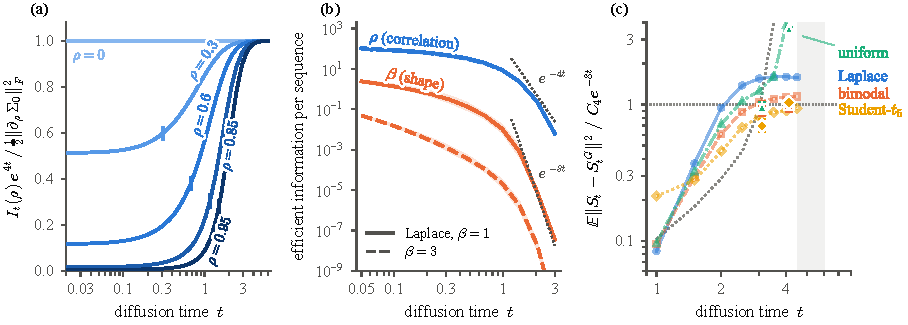
\includegraphics[width=\textwidth]{fig_theory.pdf}
  \caption{The paper's theory figure (Section 3), reproduced for reference. (a)
  Exact Fisher information of the Gaussian chain about $\corr$ divided by its
  asymptote $\tfrac12\Frob{\partial_\corr\Sig_0}^2e^{-4t}$, five correlations, ticks at
  $\tstar(\corr)$ (\cref{prop:att:gaussinfo,prop:att:tstar}). (b) Efficient
  information per sequence about $\corr$ (degree two) and about the shape exponent
  $\beta$ (degree four) of the generalised-Gaussian chain, from Fisher-identity scores,
  against the guides $e^{-4t}$ and $e^{-8t}$ (\cref{sec:att:information}). (c) The
  closure gap $\E\lVert\score-\Sgauss\rVert^2$ divided by $\tfrac16\Frob{\kfour}^2e^{-8t}$
  for four innovation families (\cref{prop:att:c4}), with the large-sample constants
  and the double-precision floor.}
  \label{fig:att:theory}
\end{figure}

\Cref{fig:att:theory} is the paper's Figure in Section 3. Panel (a) is
\cref{prop:att:gaussinfo}: no Monte Carlo, a closed form on a fine grid of $t$
(\code{part\_gauss} of \code{experiments/e01\_information\_decay.py}); the curves
reach one, and the tick marks show that a strongly correlated chain approaches its
asymptote later, as $\alpha^2\lmax$ requires. Panel (b) is
\cref{prop:att:info2,prop:att:info4} measured on the chain: the per-sequence scores of
the marginal likelihood are obtained by Fisher's identity through the tree-exact
recursion (\code{per\_chain\_scores} in \code{src/markov\_score/information.py}), the
outer-product matrix is inverted for the efficient information, and the slopes above
$\tstar$ are compared with $-4$ and $-8$; the constant of the shape rate is verified
to high precision only in the scalar case (E21), because the outer-product estimate on
the chain is a small residual of order-one quantities and reaches a quadrature floor.
Panel (c) is \cref{prop:att:c4}: the gap is measured by tree-exact message passing
against the LMMSE twin, divided by the predicted constant, on a domain wide enough
for each family's sample (E18), with the bootstrap intervals from many sequences
because the per-sequence gap is heavy-tailed (a degree-six polynomial in nearly
Gaussian variables). The uniform family, with the smallest constant, reaches the
double-precision floor of the posterior means first. All numbers are in the paper;
none is repeated here.

\section{Worked examples}
\label{sec:att:examples}

\begin{example}[The scalar Laplace law]
\label{ex:att:laplace}
A unit-variance Laplace variable has excess kurtosis $3$, so $\kappa_4=3$ and the
constant of \cref{eq:att:scoregap} is $\kappa_4^2/6=1.5$. The leading term of the score
gap is $\tfrac{3}{6}\Hen3(x)e^{-4t}=\tfrac12(x^3-3x)e^{-4t}$; at $x=2$ and $t=1$ it is
$\tfrac12\cdot2\cdot e^{-4}=0.0183$, against a twin score of $-2$. The expected squared
gap at $t=2$ is $1.5\,e^{-16}=1.5\times1.13\times10^{-7}=1.7\times10^{-7}$, and since
the score energy at that level is close to one (\cref{prop:ou:energy}), the relative
score error of the twin is about $\sqrt{1.7\times10^{-7}}=4\times10^{-4}$.
\end{example}

\begin{example}[The shape constant at the Gaussian member]
\label{ex:att:shape}
The generalised Gaussian $\innov_\beta\propto e^{-|\varepsilon/s_\beta|^\beta}$ at unit
variance has excess kurtosis $\kappa(\beta)=\Gamma(5/\beta)\Gamma(1/\beta)/\Gamma(3/\beta)^2-3$.
Its derivative at the Gaussian member $\beta=2$ can be done by hand with the digamma
recursion $\psi(x+1)=\psi(x)+1/x$:
$\frac{\dd}{\dd\beta}\log(\kappa+3)=\beta^{-2}[-5\psi(5/\beta)-\psi(1/\beta)+6\psi(3/\beta)]$,
and at $\beta=2$, with $\psi(5/2)=\psi(1/2)+2+\tfrac23$ and $\psi(3/2)=\psi(1/2)+2$,
the bracket is $(-5-1+6)\psi(\tfrac12)-\tfrac{40}3+12=-\tfrac43$, so the derivative
of the logarithm is $-\tfrac13$ and $\partial_\beta\kappa|_{\beta=2}=3\times(-\tfrac13)=-1$
exactly. In the scalar case \cref{eq:att:info4} therefore predicts
$I_t(\beta)=\tfrac1{24}e^{-8t}(1+O(e^{-2t}))$ at the Gaussian member: an information of
one part in twenty-four times $e^{-8t}$ per observation. The paper's E21 checks this
constant by untruncated quadrature (Appendix E).
\end{example}

\begin{example}[The two-site Gaussian chain, exactly]
\label{ex:att:twosite}
For $\nsites=2$, $\Sig_0=\begin{psmallmatrix}1&\corr\\\corr&1\end{psmallmatrix}$ and
$\partial_\corr\Sig_0=\begin{psmallmatrix}0&1\\1&0\end{psmallmatrix}$, so
$\tfrac12\Frob{\partial_\corr\Sig_0}^2=1$. With $\Sig_t=\begin{psmallmatrix}1&\alpha^2\corr\\\alpha^2\corr&1\end{psmallmatrix}$,
$\Sig_t^{-1}\partial_\corr\Sig_t=\frac{\alpha^2}{1-\alpha^4\corr^2}\begin{psmallmatrix}-\alpha^2\corr&1\\1&-\alpha^2\corr\end{psmallmatrix}$,
whose square has trace $2\alpha^4(1+\alpha^4\corr^2)/(1-\alpha^4\corr^2)^2$, so by
\cref{prop:att:gaussinfo}
\[
  I_t(\corr)=\frac{\alpha^4(1+\alpha^4\corr^2)}{(1-\alpha^4\corr^2)^2}=e^{-4t}\bigl(1+3\alpha^4\corr^2+O(\alpha^8)\bigr).
\]
At $\corr=0.85$ and $t=1$: $\alpha^4=e^{-4}=0.01832$ and $\alpha^4\corr^2=0.01323$, so
\[
  I_1=\frac{0.01832\times1.01323}{0.98677^2}=0.01906,
\]
four per cent above the asymptote. Here
the correction is $O(\alpha^4)$ rather than $O(\alpha^2)$ because $\tr(\Sig_0-\Id)=0$
and the first-order term of the Neumann series drops out of the trace; for the
$32$-site chain it does not, and the correction is $O(\alpha^2\lmax)$.
\end{example}

\begin{example}[The fourth-cumulant tensor of a three-site chain]
\label{ex:att:tensor}
Let $a_1\sim\normal01$, $a_2=\corr a_1+\varepsilon_2$, $a_3=\corr a_2+\varepsilon_3=\corr^2a_1+\corr\varepsilon_2+\varepsilon_3$,
with i.i.d.\ innovations of variance $\ivar=1-\corr^2$ and fourth cumulant
$\kappa_4(\varepsilon)=3\ivar^2$ (Laplace). Joint cumulants are additive over the
independent summands and $a_1$ is Gaussian, so
$\kfour[ijkl]=\kappa_4(\varepsilon)\sum_{m=2}^{\min(i,j,k,l)}\corr^{i+j+k+l-4m}$
(\code{chain\_kappa4} in \code{src/markov\_score/theory.py}). The nonzero entries up
to permutation are $\kfour[2222]=3\ivar^2$, $\kfour[2223]=3\ivar^2\corr$,
$\kfour[2233]=3\ivar^2\corr^2$, $\kfour[2333]=3\ivar^2\corr^3$ and
$\kfour[3333]=3\ivar^2(\corr^4+1)$. Over ordered tuples the Frobenius norm is
\[
  \Frob{\kfour}^2=9\ivar^4\bigl[1+4\corr^2+6\corr^4+4\corr^6+(1+\corr^4)^2\bigr],
\]
the multiplicities being $1,4,6,4,1$. At $\corr=0.85$: $\ivar=0.2775$, $\ivar^4=0.00593$,
$\corr^2=0.7225$, $\corr^4=0.5220$, $\corr^6=0.3772$; the bracket is
$1+2.890+3.132+1.509+2.317=10.85$, so $\Frob{\kfour}^2=9\times0.00593\times10.85=0.579$
and $\tfrac16\Frob{\kfour}^2=0.0965$. The same recipe at $\nsites=32$ gives the
constant the paper quotes for the Laplace chain (Section 3, ``Verification with the
exact score''), which grows linearly in $\nsites$ away from the first site.
\end{example}

\begingroup\setlength{\emergencystretch}{2em}
\where{Section 3 of the paper (Theorems 2--4, Assumption (E), Corollary 5, the
crossover and heavy-tail paragraphs, the Edgeworth paragraph) and Appendix A
(the proofs). Experiments: E01 (Gaussian closed form, shape information on the chain,
closure gap), E16 (Edgeworth correction), E18 (closure constant and heavy tails on
wide domains, untruncated scalar quadrature), E21 (information curve at $\corr=0.5$
and the scalar shape constant). Code: \code{src/\allowbreak markov\_score/\allowbreak theory.py}
(\code{he}, \code{chain\_\allowbreak covariance}, \code{chain\_\allowbreak kappa4}, \code{gaussian\_\allowbreak chain\_\allowbreak fisher},
\code{score\_\allowbreak gap\_\allowbreak constant}, \code{shape\_\allowbreak information\_\allowbreak constant},
\code{correlation\_\allowbreak information\_\allowbreak constant}, \code{crossover\_\allowbreak time}),
\code{src/\allowbreak markov\_score/\allowbreak information.py} (\code{per\_\allowbreak chain\_\allowbreak scores},
\code{outer\_\allowbreak product\_\allowbreak information}, \code{efficient\_\allowbreak information}),
\code{experiments/\allowbreak e01\_information\_decay.py},
\code{experiments/\allowbreak e16\_edgeworth\_oracle.py},
\code{experiments/\allowbreak e18\_closure\_wide.py},
\code{experiments/\allowbreak e21\_information\_curve.py}; the Lean targets for the
constants are listed in \code{lean/\allowbreak README.md}. Audit: \code{docs/\allowbreak SCIENCE\_\allowbreak AUDIT.md},
\code{reports/\allowbreak audit-\allowbreak 2026-\allowbreak 09-\allowbreak 18.tex}, Section 3.}
\endgroup

\paragraph{References.}
F.~G.~Mehler, 1866, ``Ueber die Entwicklung einer Function von beliebig vielen
Variabeln nach Laplaceschen Functionen h\"oherer Ordnung'', Journal f\"ur die reine und
angewandte Mathematik 66, 161--176.
S.~Janson, 1997, \emph{Gaussian Hilbert Spaces}, Cambridge University Press (Wick
products and Wick's theorem, Chapter 3).
P.~McCullagh, 1987, \emph{Tensor Methods in Statistics}, Chapman and Hall (joint
cumulants, the Leonov--Shiryaev formula, Edgeworth expansions).
A.~W.~van der Vaart, 1998, \emph{Asymptotic Statistics}, Cambridge University Press
(local asymptotic minimax theorem, Chapter 8).
D.~Guo, S.~Shamai and S.~Verd\'u, 2005, ``Mutual information and minimum mean-square
error in Gaussian channels'', IEEE Transactions on Information Theory 51, 1261--1282.
A.~Katsevich and A.~S.~Bandeira, 2023, ``Likelihood maximization and moment matching
in low SNR Gaussian mixture models'', Communications on Pure and Applied Mathematics
76, 788--842.


\part{Exact inference}
\chapter{Factor graphs and belief propagation}
\label{ch:factor-graphs-bp}
% colours of the paper's house palette (tools/figstyle.py), defined locally so this part
% compiles inside the compendium preamble, which does not load the paper's main.tex
\definecolor{bpBlue}{HTML}{2A78D6}
\definecolor{bpInk}{HTML}{52514E}
\definecolor{bpFill}{HTML}{E1E0DC}

The paper's central computational claim is that the score of a non-Gaussian,
correlated law in $\nsites$ dimensions is available exactly, by ``one forward--backward
sweep of functional message passing''. This chapter builds the objects in that sentence
from scratch: what a factor graph is, what the sum-product algorithm does on it, why the
algorithm is exact when the graph is a tree, and why conditioning the chain prior on
coordinatewise noised observations leaves a tree. It then specialises the general
algorithm to the two message sweeps of the paper's equation for $\lmsg_i$ and $\rmsg_i$
(Appendix B, the equation labelled \emph{bp}), reads off the site marginals, the pairwise
marginals and the evidence, and places the recursion next to its two classical
relatives, the forward--backward algorithm for hidden Markov models and the Kalman
smoother.

\section{Graphical models and factor graphs}

\subsection{Factorised functions}

Let $a=(a_1,\dots,a_\nsites)$ be a vector of variables, each taking values in a set
$\mathcal{A}$ (a finite alphabet, or $\Reals$). A \term{factorisation} of a
non-negative function $f$ of $a$ is a representation
\begin{equation}
  f(a)=\prod_{\alpha\in\mathcal{F}}\psi_\alpha(a_{\partial\alpha}),
  \label{eq:bp-factorisation}
\end{equation}
where $\mathcal{F}$ is a finite index set of \term{factors}, each factor $\alpha$ has a
\term{scope} $\partial\alpha\subseteq\{1,\dots,\nsites\}$, and $a_{\partial\alpha}$ is the
sub-vector of the variables in that scope. The \term{factor graph} of the factorisation
is the bipartite graph with one \term{variable node} per index $i$, one \term{factor
node} per factor $\alpha$, and an edge between $i$ and $\alpha$ whenever
$i\in\partial\alpha$. A factor with a scope of size one is called
\term{unary}; a scope of size two is \term{pairwise}.

When $f$ is a probability density up to a constant, $p(a)=f(a)/Z$ with
$Z=\int f(a)\dd a$, the factor graph is a \term{graphical model} of $p$. The constant
$Z$ is the \term{normaliser}, also called the \term{partition function} in physics and,
when $f$ is a joint density of data and latent variables evaluated at the observed data,
the \term{evidence} or \term{marginal likelihood}.

\begin{example}[The chain prior]
\label{ex:bp-chain-prior}
The paper's clean law, its Section 2, equation \emph{prior}, is
$\Pz(\va)=\mu(a_1)\prod_{i=2}^{\nsites}\kernel(a_i\mid a_{i-1})$. It is a factorisation
with one unary factor $\mu$ of scope $\{1\}$ and $\nsites-1$ pairwise factors
$\kernel(\cdot\mid\cdot)$ of scopes $\{i-1,i\}$. Its factor graph is a path: variable
nodes $a_1,a_2,\dots,a_\nsites$ with a factor node between each consecutive pair, and
a dangling unary factor at $a_1$. Here $Z=1$ because each $\kernel(\cdot\mid a)$
integrates to one.
\end{example}

\subsection{Conditional independence}

The factor graph encodes which variables are conditionally independent of which. The
statement we need is the following. If removing the variable node $a_i$ (together with
its edges) disconnects the graph into components $\mathcal{C}_1,\dots,\mathcal{C}_r$,
then under $p$ the groups of variables in different components are conditionally
independent given $a_i$. The proof is one line: every factor lies inside one component
(its scope, minus $i$, is connected through the factor node), so
$f(a)=\prod_j g_j(a_{\mathcal{C}_j},a_i)$, and a joint density that is a product of
functions of the separate groups (each also depending on $a_i$) is, given $a_i$, a
product density.

Applied to the path of \cref{ex:bp-chain-prior}, removing $a_i$ separates the past
$\{a_1,\dots,a_{i-1}\}$ from the future $\{a_{i+1},\dots,a_\nsites\}$: this is the
\term{Markov property}, and it is the only use we make of the word ``Markov''.

\subsection{Trees, and why marginalisation is hard in general}

A factor graph is a \term{tree} when it is connected and has no cycles. A path is a
tree. The \term{marginal} of $p$ at a variable $i$ is
$p_i(a_i)=\frac1Z\int f(a)\dd a_{\setminus i}$, integrating over every variable but the
$i$-th. Written out on a finite alphabet of size $\ngrid$, the integral is a sum over
$\ngrid^{\nsites-1}$ configurations, which for the paper's $\ngrid=401$ and $\nsites=32$
is not a computation. Every algorithm in this chapter is a way of organising that sum
so that it costs $O(\nsites\ngrid^2)$ instead, and the organisation is possible exactly
because the graph is a tree.

\section{The sum-product algorithm}

\subsection{Messages}

The \term{sum-product algorithm}, also called \term{belief propagation}, passes two
kinds of functions along the edges of the factor graph. For an edge between variable
$i$ and factor $\alpha$:
\begin{align}
  \text{variable to factor:}\qquad
  m_{i\to\alpha}(a_i)&=\prod_{\beta\in\partial i\setminus\{\alpha\}} m_{\beta\to i}(a_i),
  \label{eq:bp-v2f}\\
  \text{factor to variable:}\qquad
  m_{\alpha\to i}(a_i)&=\int\psi_\alpha(a_{\partial\alpha})
    \prod_{j\in\partial\alpha\setminus\{i\}} m_{j\to\alpha}(a_j)\dd a_{\partial\alpha\setminus i},
  \label{eq:bp-f2v}
\end{align}
where $\partial i$ is the set of factors whose scope contains $i$. An empty product is
$1$, so a leaf variable (one attached to a single factor) sends the constant message
$1$, and a leaf factor (a unary factor) sends its own function
$m_{\alpha\to i}(a_i)=\psi_\alpha(a_i)$. The names are literal: a message is a function
of the variable at the edge's variable end, and \cref{eq:bp-f2v} sums (integrates) a
product.

On a tree, every message can be computed once and in a definite order: root the tree
anywhere, compute messages from the leaves towards the root, then from the root back
towards the leaves. Each edge carries one message in each direction, and each message
is computed after all the messages it depends on. The \term{belief} at a variable and at
a factor are then
\begin{equation}
  b_i(a_i)\propto\prod_{\alpha\in\partial i} m_{\alpha\to i}(a_i),\qquad
  b_\alpha(a_{\partial\alpha})\propto\psi_\alpha(a_{\partial\alpha})
   \prod_{j\in\partial\alpha} m_{j\to\alpha}(a_j).
  \label{eq:bp-beliefs}
\end{equation}

\subsection{Exactness on a tree}

\begin{theorem}[Sum-product is exact on a tree]
\label{thm:bp-exact}
Let the factor graph of \cref{eq:bp-factorisation} be a tree. Then the beliefs of
\cref{eq:bp-beliefs} are the exact marginals: $b_i=p_i$ and $b_\alpha=p_{\partial\alpha}$,
where $p_{\partial\alpha}$ is the marginal of $p$ on the scope of $\alpha$. Moreover, for
every variable $i$, $Z=\int\prod_{\alpha\in\partial i} m_{\alpha\to i}(a_i)\dd a_i$.
\end{theorem}

\begin{proof}
The proof is an induction on subtrees, and it rests on one fact about integrals of
products: the \term{distributive law}, $\int g(u)h(v)\dd u\dd v=\int g\dd u\int h\dd v$
when the two factors depend on disjoint sets of variables.

Fix an edge $(i,\alpha)$ and delete it. Because the graph is a tree, this splits it into
two subtrees; call $T_{\alpha\to i}$ the one containing $\alpha$ and $T_{i\to\alpha}$ the one
containing $i$. Write $F_{\alpha\to i}(a_i)$ for the integral, over every variable of
$T_{\alpha\to i}$ other than $a_i$, of the product of all factors in $T_{\alpha\to i}$; and
$F_{i\to\alpha}(a_i)$ likewise for $T_{i\to\alpha}$ (the factors on the $i$ side other than
$\alpha$). We claim
\begin{equation}
  m_{\alpha\to i}=F_{\alpha\to i},\qquad m_{i\to\alpha}=F_{i\to\alpha}.
  \label{eq:bp-claim}
\end{equation}
The claim is proved by induction on the number of nodes in the subtree behind the
message. If $T_{\alpha\to i}$ consists of $\alpha$ alone, then $\alpha$ is unary and both
sides equal $\psi_\alpha(a_i)$. If $T_{i\to\alpha}$ consists of $i$ alone, both sides are
$1$. Otherwise, suppose the claim holds for all smaller subtrees. The subtree
$T_{\alpha\to i}$ is $\alpha$ together with, for each $j\in\partial\alpha\setminus\{i\}$, the
subtree $T_{j\to\alpha}$; these subtrees are disjoint (no cycles) and share no variables
with one another (a shared variable would be a cycle through $\alpha$). Hence the product
of all factors in $T_{\alpha\to i}$ is $\psi_\alpha\prod_j(\text{factors of }T_{j\to\alpha})$,
and integrating out the variables of each $T_{j\to\alpha}$ other than $a_j$ can be done
separately by the distributive law, giving $\psi_\alpha\prod_j F_{j\to\alpha}(a_j)$; the
remaining integral over $a_{\partial\alpha\setminus i}$ is exactly \cref{eq:bp-f2v} once
$F_{j\to\alpha}=m_{j\to\alpha}$ by the induction hypothesis. The variable-to-factor case
is the same argument with the subtrees $T_{\beta\to i}$, $\beta\in\partial i\setminus\{\alpha\}$,
which share only the variable $a_i$; no integral is needed and
\cref{eq:bp-v2f} follows.

Now take a variable $i$. The whole graph is the union of the subtrees $T_{\alpha\to i}$,
$\alpha\in\partial i$, which pairwise share only $a_i$. By the distributive law again,
$\int f(a)\dd a_{\setminus i}=\prod_{\alpha\in\partial i}F_{\alpha\to i}(a_i)$, and by
\cref{eq:bp-claim} this is the unnormalised belief. Integrating once more over $a_i$
gives $Z$. For a factor $\alpha$, the whole graph is $\alpha$ together with the subtrees
$T_{j\to\alpha}$, $j\in\partial\alpha$, sharing no variables, and the same reasoning gives
$b_\alpha=p_{\partial\alpha}$.
\end{proof}

Three remarks on the theorem. First, nothing in the proof depends on the variables
being discrete: on $\Reals$ the messages are functions and the sums are integrals,
which is what the paper means by \emph{functional} message passing. Second, the
proof shows that the belief at a factor integrates, over the variables of the factor
other than $i$, to the belief at $i$: beliefs are \term{locally consistent}. Third,
on a graph with cycles the messages of \cref{eq:bp-v2f,eq:bp-f2v} still make sense
and can be iterated (\term{loopy belief propagation}), but the induction fails at the
first cycle and the beliefs are approximations. The paper's claim is that its
inference is \emph{tree-exact}: the posterior graph is a tree, so no such approximation
is made.

\section{The chain posterior of the paper}

\subsection{Conditioning adds only unary factors}

The observation model is the coordinatewise channel of the paper's equation
\emph{channel}: given the clean chain $\va$, the coordinates of
$\vx=e^{-t}\va+\sqrt{\Dt}\vz$ are independent, each with density
$\normal{e^{-t}a_i}{\Dt}$ in $x_i$. By Bayes' rule,
\begin{equation}
  p_t(\va\mid\vx)=\frac{\Pz(\va)\prod_{i=1}^{\nsites}\like(x_i\mid a_i)}{\Pt(\vx)},\qquad
  \like(x_i\mid a_i)=\frac{1}{\sqrt{2\pi\Dt}}\exp\!\Bigl[-\frac{(x_i-e^{-t}a_i)^2}{2\Dt}\Bigr].
  \label{eq:bp-posterior}
\end{equation}
Compared with the prior, the numerator has one extra factor per site, each of scope
$\{i\}$: a \term{unary likelihood factor}. No factor couples two latent variables that
were not already coupled. The factor graph of the posterior is therefore the prior's
path with a unary factor hanging from every variable node; it is still a tree
(\cref{fig:bp-chain}). This is the whole content of the sentence ``conditioning leaves
the posterior factor graph a tree''. It would fail for a channel that mixed coordinates
(a non-diagonal noise covariance would add pairwise factors among the $a_i$, closing
cycles), and it holds for any prior whose graph is a tree, not only for a path.

\begin{figure}[t]
  \centering
  \begin{tikzpicture}[
    x=1cm, y=1cm, font=\small,
    lat/.style={circle, draw=bpInk, line width=0.5pt, fill=white, minimum size=6.2mm, inner sep=0pt},
    obs/.style={circle, draw=bpInk, line width=0.5pt, fill=bpFill, minimum size=6.2mm, inner sep=0pt},
    fac/.style={rectangle, draw=bpInk, line width=0.5pt, fill=bpInk, minimum size=2.2mm, inner sep=0pt},
    ufac/.style={rectangle, draw=bpInk, line width=0.5pt, fill=white, minimum size=2.2mm, inner sep=0pt},
    edge/.style={draw=bpInk, line width=0.5pt},
    gap/.style={inner sep=0pt, minimum size=6.2mm, text=bpInk},
    msg/.style={-{Latex[length=1.8mm, width=1.4mm]}, line width=0.8pt, draw=bpBlue},
    rowlab/.style={anchor=east, inner sep=0pt},
  ]
    \def\dx{1.55}
    \def\ya{1.5}\def\yl{0.75}\def\yx{0.0}
    \foreach \i/\al in {1/a_1, 2/a_2, 4/a_i, 6/a_\nsites} {
      \node[lat] (a\i) at (\dx*\i, \ya) {$\al$};
    }
    \foreach \i in {3,5} { \node[gap] (a\i) at (\dx*\i, \ya) {$\cdots$}; }
    \foreach \i/\j in {1/2,2/3,3/4,4/5,5/6} {
      \node[fac] (k\i) at ($(a\i)!0.5!(a\j)$) {};
      \draw[edge] (a\i) -- (k\i) -- (a\j);
    }
    \foreach \i/\xl in {1/x_1, 2/x_2, 4/x_i, 6/x_\nsites} {
      \node[ufac] (l\i) at (\dx*\i, \yl) {};
      \node[obs]  (x\i) at (\dx*\i, \yx) {$\xl$};
      \draw[edge] (a\i) -- (l\i) -- (x\i);
    }
    \foreach \i in {3,5} { \node[gap] (x\i) at (\dx*\i, \yx) {$\cdots$}; }
    \node[fac] (m1) at (\dx*1-0.75, \ya) {};
    \draw[edge] (m1) -- (a1);
    \node[anchor=east, inner sep=1pt, font=\footnotesize] at (\dx*1-0.85, \ya) {$\mu$};
    \node[rowlab] at (\dx-1.35, \ya+0.55) {$\kernel(a_i\!\mid\! a_{i-1})$};
    \node[rowlab] at (\dx-1.35, \yl) {$\like(x_i\!\mid\! a_i)$};
    \node[rowlab] at (\dx-1.35, \yx) {$\vx_t$};
    \draw[msg] ($(a1)+(0.35,0.55)$) -- ($(a4)+(-0.4,0.55)$)
      node[midway, above=1pt, text=bpBlue, inner sep=1pt] {$\lmsg$};
    \draw[msg] ($(a6)+(-0.35,0.55)$) -- ($(a4)+(0.4,0.55)$)
      node[midway, above=1pt, text=bpBlue, inner sep=1pt] {$\rmsg$};
  \end{tikzpicture}
  \caption{The factor graph of the chain posterior, drawn as in the paper's Figure 1.
  Latent sites (white circles) are joined by the transition factors $\kernel$ (filled
  squares) and, at the left end, by the initial factor $\mu$. Conditioning attaches one
  unary likelihood factor (open square) per site, joining $a_i$ to its own observation
  $x_i$ (shaded circle), and adds no edge among the latent variables. The graph is a
  tree, so the forward sweep $\protect\lmsg$ and the backward sweep $\protect\rmsg$ of the sum-product
  algorithm are exact; they meet at the query site $i$.}
  \label{fig:bp-chain}
\end{figure}

\subsection{From the general rules to the two sweeps}

Specialise \cref{eq:bp-v2f,eq:bp-f2v} to \cref{fig:bp-chain}. Each latent variable $a_i$
has at most three neighbouring factors: the transition factor on its left, the
transition factor on its right, and its unary likelihood. Write $\kernel_{i}$ for the
factor between $a_{i-1}$ and $a_i$ (with $\kernel_1=\mu$ the unary initial factor).
Going left to right, the message that $\kernel_{i}$ sends into $a_i$ is, by
\cref{eq:bp-f2v}, an integral over $a_{i-1}$ of $\kernel(a_i\mid a_{i-1})$ times the
message $a_{i-1}$ sends into $\kernel_i$; and that message is, by \cref{eq:bp-v2f}, the
product of what $a_{i-1}$ receives from its other two neighbours, its own unary factor
$\like(x_{i-1}\mid\cdot)$ and the transition factor on its left. Naming
$\lmsg_i(a)=m_{\kernel_i\to a_i}(a)$, this reads
\begin{equation}
  \lmsg_1(a)=\mu(a),\qquad
  \lmsg_i(a)=\int\kernel(a\mid a')\,\like(x_{i-1}\mid a')\,\lmsg_{i-1}(a')\dd a',\quad i\ge2.
  \label{eq:bp-forward}
\end{equation}
Going right to left, name $\rmsg_i(a)=m_{\kernel_{i+1}\to a_i}(a)$ the message that the
transition factor on the right of $a_i$ sends into $a_i$; for the last site there is
no such factor and $\rmsg_\nsites\equiv1$ (an empty product). The same two rules give
\begin{equation}
  \rmsg_\nsites(a)=1,\qquad
  \rmsg_i(a)=\int\kernel(a''\mid a)\,\like(x_{i+1}\mid a'')\,\rmsg_{i+1}(a'')\dd a'',\quad i\le\nsites-1.
  \label{eq:bp-backward}
\end{equation}
These are, up to the proportionality signs discussed in \cref{sec:bp-normalisation},
the two lines of the paper's equation \emph{bp}. The paper's convention for
$\lmsg_1$ differs from \cref{eq:bp-forward} in one cosmetic respect: it writes
$\lmsg_1\equiv1$ and treats $\mu$ as if it were part of the first site's unary factor.
The code follows \cref{eq:bp-forward}, with \code{L[0] = exp(log\_mu)} and
\code{R[-1] = 1} in \code{src/markov\_score/bp\_grid.py}. Note the asymmetry of the
kernel's arguments: forward, the integration variable is the \emph{conditioning}
argument of $\kernel$; backward, it is the \emph{conditioned} one. The transition
matrix on a grid, $\kernel[k,l]=\kernel(\gridpt{k}\mid\gridpt{l})$ with column index
the parent, enters the forward sweep as $\kernel$ and the backward sweep as
$\kernel^{\!\top}$, which is exactly what the code does.

Two conventions are worth fixing, because both appear in the literature. The messages
\cref{eq:bp-forward,eq:bp-backward} \emph{exclude} the unary factor of the site they
arrive at; they are the factor-to-variable messages of the general algorithm. The
alternative convention (the ``filtered'' forward variable of the HMM literature)
multiplies the local likelihood in and would be $\lmsg_i\like$. The paper and the code
use the excluded form, so that the local factor appears once, explicitly, in every
formula below.

\subsection{Site marginals, pairwise marginals and the evidence}

By \cref{eq:bp-beliefs}, the belief at site $i$ is the product of what it receives from
its three neighbours,
\begin{equation}
  p_t(a_i\mid\vx)=\frac{\lmsg_i(a_i)\,\like(x_i\mid a_i)\,\rmsg_i(a_i)}{Z_i},\qquad
  Z_i=\int\lmsg_i\like(x_i\mid\cdot)\rmsg_i\dd a_i,
  \label{eq:bp-site}
\end{equation}
and by \cref{thm:bp-exact} it is the exact posterior marginal. The paper's phrase
``site marginals $\propto\lmsg_i\like\rmsg_i$'' is this line. The belief at the
transition factor between $a_{i-1}$ and $a_i$ is
\begin{equation}
  p_t(a_{i-1},a_i\mid\vx)=\frac{\lmsg_{i-1}(a_{i-1})\,\like(x_{i-1}\mid a_{i-1})\,
    \kernel(a_i\mid a_{i-1})\,\like(x_i\mid a_i)\,\rmsg_i(a_i)}{Z_{i-1,i}},
  \label{eq:bp-pair}
\end{equation}
the exact \term{pairwise marginal}, whose two single-site margins are \cref{eq:bp-site}
at $i-1$ and at $i$ (local consistency). The pairwise marginals are what the
expectation--maximisation chapter (\cref{ch:em-through-noise}) sums into the expected
transition statistic $\Xis$; they come from the same two sweeps at no extra cost beyond
the outer products.

The normaliser is available at any site, $Z_i=\Pt(\vx)$ for every $i$, because every
$Z_i$ equals $\int\Pz(\va)\prod_j\like(x_j\mid a_j)\dd\va$ by the proof of
\cref{thm:bp-exact}; the same holds for every $Z_{i-1,i}$. In particular the forward
sweep alone gives it, as $Z_\nsites=\int\lmsg_\nsites\like(x_\nsites\mid\cdot)\dd a$ once
$\rmsg_\nsites\equiv1$. This number, $\log\Pt(\vx)$, is the \term{log-evidence}: the
marginal log-likelihood of one noised sequence under the chain prior, which the paper's
Section 4 maximises over the parameters of the kernel and which its Appendix E uses,
summed over a held-out bundle, as an oracle-free model-selection criterion.

\subsection{From the marginal to the score}

The paper needs one number per site, the posterior mean
$\pmeansite{i}=\int a_i\,p_t(a_i\mid\vx)\dd a_i$, because Tweedie's identity
(the chapter on the Ornstein--Uhlenbeck channel) converts it into the score,
$\score(\vx,t)_i=-(x_i-e^{-t}\pmeansite{i})/\Dt$. Thus the whole of ``the exact score''
is: two sweeps, $\nsites$ one-dimensional integrals for the means, and one subtraction
per site. The word ``exact'' refers to \cref{thm:bp-exact}; what is not exact is the
numerical representation of the messages, which is the subject of
\cref{ch:grid-quadrature}.

\subsection{Normalisation and the log-normaliser}
\label{sec:bp-normalisation}

Messages are defined up to a positive constant: multiplying $\lmsg_i$ by $c$ multiplies
every later forward message and every belief involving it by $c$, and the
normalised beliefs \cref{eq:bp-site,eq:bp-pair} are unchanged. This is why the paper
writes $\propto$ in its recursion. Numerically, unnormalised messages on a long chain
underflow or overflow (each step multiplies by a likelihood of order
$1/\sqrt{2\pi\Dt}$ and by a kernel of order $1/\sqrt{\ivar}$), so an implementation
rescales each message to unit mass and keeps the discarded constants:
\begin{equation}
  \tilde{\lmsg}_{i}=\frac{\lmsg_i}{c_i},\qquad c_i=\int\lmsg_i\dd a,\qquad
  \log\Pt(\vx)=\sum_{i=2}^{\nsites}\log c_i+\log\int\tilde{\lmsg}_\nsites\like(x_\nsites\mid\cdot)\dd a,
  \label{eq:bp-logZ}
\end{equation}
where each $c_i$ is computed from the \emph{already rescaled} previous message, so
that the product of the $c_i$ is the total constant removed. The log-evidence is thus
assembled from a sum of logarithms and never as a product of small numbers.
\Cref{ch:grid-quadrature} gives the grid version, including the constants of the
likelihood factors that the implementation removes for stability and restores at the
end.

\subsection{Cost}

On a grid of $\ngrid$ points, a message is a vector of length $\ngrid$ and a
transition integral is a matrix--vector product with the $\ngrid\times\ngrid$ matrix
$\kernel[k,l]$, costing $O(\ngrid^2)$. The forward sweep performs $\nsites-1$ of them,
the backward sweep the same, and the beliefs cost $O(\nsites\ngrid)$. The total is
$O(\nsites\ngrid^2)$ per sequence and per noise level, as the paper states in its
conclusion, and it is linear in the chain length: this is why the length-extrapolation
study of the paper's Section 5 costs nothing extra at $\nsites=256$. For a batch of
$B$ sequences the matrix--vector products become matrix--matrix products
$(\ngrid\times\ngrid)(\ngrid\times B)$, which is how \code{grid\_bp\_batch} in
\code{src/markov\_score/bp\_grid.py} organises the computation.

\section{Three names for one recursion}

\paragraph{Forward--backward for hidden Markov models.}
When the state space is a finite set of $\ngrid$ symbols, \cref{eq:bp-forward,eq:bp-backward}
are the forward and backward recursions of Baum and colleagues (1970) and Rabiner's
tutorial (1989), usually written for the filtered variable
$\alpha_i(k)=P(a_i=k,x_1,\dots,x_i)$ and the backward variable
$\beta_i(k)=P(x_{i+1},\dots,x_\nsites\mid a_i=k)$. In our notation
$\alpha_i=\lmsg_i\like(x_i\mid\cdot)$ and $\beta_i=\rmsg_i$; the posterior at a site is
$\alpha_i\beta_i/\Pt(\vx)$ and the pairwise posterior is
$\alpha_{i-1}\kernel\like\beta_i/\Pt(\vx)$, both as above. The pairwise posteriors summed
over sites are the ``expected transition counts'' of the Baum--Welch algorithm, and
their continuous analogue on the grid is exactly the paper's $\Xis$. The paper's
recursion is therefore not a new algorithm; the paper says so in its related work,
citing Baum and Rabiner.

\paragraph{The Kalman smoother.}
When $\mu$, $\kernel$ and $\like$ are all Gaussian, every message is Gaussian (a
product of Gaussians is Gaussian, and the convolution of a Gaussian with a Gaussian
kernel is Gaussian), so each message is carried by two numbers, a mean and a variance,
or equivalently a precision and an information vector. The forward sweep is then the
Kalman filter and the combination of forward and backward messages is the
Rauch--Tung--Striebel smoother. \Cref{ch:gaussian-closure-lmmse} writes out the two
moment maps and proves the paper's Proposition 1, which says that projecting every
message onto a Gaussian, for \emph{any} innovation law with the same variance,
reproduces this smoother. The implementation of the Gaussian case is
\code{gaussian\_chain\_bp} in \code{src/markov\_score/bp\_gaussian.py}.

\paragraph{Functional message passing and Kitagawa's grid smoother.}
When the state is continuous and non-Gaussian, the messages are genuine functions on
$\Reals$ and have no finite parametrisation. The paper calls the recursion
``functional message passing'' to stress that the algorithm is defined at the level of
functions, before any discretisation, and ``tree-exact inference'' to stress that the
only approximation is in representing those functions. Representing them by their
values on a grid and replacing integrals by quadrature is Kitagawa's non-Gaussian
smoother (1987), which the paper also cites. The phrase ``the score'' throughout the
paper means: the posterior mean obtained by this recursion, evaluated on a grid whose
adequacy is measured (\cref{ch:grid-quadrature}), inserted into Tweedie's identity.

\section{A worked example: three sites, three states}
\label{sec:bp-example}

Take $\nsites=3$ sites and a three-point alphabet $\{\gridpt{1},\gridpt{2},\gridpt{3}\}=\{-1,0,1\}$
with no quadrature weights (a finite-state model, so that every integral is a sum).
Let the initial law, the transition matrix and the three likelihood rows be
\[
  \mu=\begin{pmatrix}0.25\\0.5\\0.25\end{pmatrix},\qquad
  \kernel=\begin{pmatrix}0.6&0.2&0.1\\0.3&0.6&0.3\\0.1&0.2&0.6\end{pmatrix},\qquad
  \ell_1=\begin{pmatrix}0.2\\0.5\\0.3\end{pmatrix},\;
  \ell_2=\begin{pmatrix}0.1\\0.3\\0.6\end{pmatrix},\;
  \ell_3=\begin{pmatrix}0.4\\0.4\\0.2\end{pmatrix},
\]
where $\kernel[k,l]$ is the probability of moving from state $l$ (column) to state $k$
(row), so the columns sum to one, and $\ell_i[k]$ (the unary factor $\like(x_i\mid\gridpt{k})$ of the chapter, written as a plain vector here) is the likelihood of the $i$-th
observation given $a_i=\gridpt{k}$ (any positive numbers; they are not normalised over
$k$ and need not be).

\emph{Forward sweep.} $\lmsg_1=\mu$. The message into site 2 is
$\lmsg_2=\kernel(\lmsg_1\circ\ell_1)$, with $\circ$ the elementwise product:
$\lmsg_1\circ\ell_1=(0.05,\,0.25,\,0.075)$, and
\[
  \lmsg_2=\begin{pmatrix}0.6\cdot0.05+0.2\cdot0.25+0.1\cdot0.075\\
                         0.3\cdot0.05+0.6\cdot0.25+0.3\cdot0.075\\
                         0.1\cdot0.05+0.2\cdot0.25+0.6\cdot0.075\end{pmatrix}
        =\begin{pmatrix}0.0875\\0.1875\\0.1\end{pmatrix}.
\]
Then $\lmsg_2\circ\ell_2=(0.00875,\,0.05625,\,0.06)$ and
$\lmsg_3=\kernel(\lmsg_2\circ\ell_2)=(0.0225,\,0.054375,\,0.048125)$.

\emph{Backward sweep.} $\rmsg_3=(1,1,1)$. Then
$\rmsg_2=\kernel^{\!\top}(\rmsg_3\circ\ell_3)=\kernel^{\!\top}(0.4,0.4,0.2)$: the first
entry is $0.6\cdot0.4+0.3\cdot0.4+0.1\cdot0.2=0.38$, and altogether
$\rmsg_2=(0.38,\,0.36,\,0.28)$. Next $\rmsg_2\circ\ell_2=(0.038,\,0.108,\,0.168)$ and
$\rmsg_1=\kernel^{\!\top}(\rmsg_2\circ\ell_2)=(0.072,\,0.106,\,0.137)$.

\emph{Evidence.} From the end of the forward sweep,
$Z=\sum_k\lmsg_3[k]\ell_3[k]=0.0225\cdot0.4+0.054375\cdot0.4+0.048125\cdot0.2=0.040375$.
The same number is obtained at site 1, $\sum_k\mu[k]\ell_1[k]\rmsg_1[k]
=0.25\cdot0.2\cdot0.072+0.5\cdot0.5\cdot0.106+0.25\cdot0.3\cdot0.137=0.040375$, and at
site 2, as \cref{thm:bp-exact} requires.

\emph{Site marginals.} At site 1 the unnormalised belief is
$\mu\circ\ell_1\circ\rmsg_1=(0.0036,\,0.0265,\,0.010275)$; dividing by $Z$ gives
$p(a_1\mid\vx)=(0.0892,\,0.6564,\,0.2545)$ and posterior mean
$-0.0892+0.2545=0.1653$. At site 2 the unnormalised belief is
\[
  \lmsg_2\circ\ell_2\circ\rmsg_2=(0.003325,\,0.02025,\,0.0168),
\]
so that the normalised marginal is $p(a_2\mid\vx)=(0.0824,\,0.5015,\,0.4161)$, with
mean $0.3337$. At site 3 the same steps give $p(a_3\mid\vx)=(0.2229,\,0.5387,\,0.2384)$
and the mean $0.0155$. Enumerating all $27$
configurations of $(a_1,a_2,a_3)$ and summing gives the same $Z$ and the same three
marginals, which is the finite version of \cref{thm:bp-exact}.

\emph{Pairwise marginal.} On the edge $(1,2)$, \cref{eq:bp-pair} gives the matrix with
entries
\[
  p(a_2=\gridpt{k},a_1=\gridpt{l}\mid\vx)=\rmsg_2[k]\,\ell_2[k]\,\kernel[k,l]\,\lmsg_1[l]\,\ell_1[l]/Z;
\]
for instance the entry $(k,l)=(2,2)$, staying at $0$, is
$0.108\cdot0.6\cdot0.25/0.040375=0.4012$, and the full matrix is
\[
  p(a_2=\gridpt{k},a_1=\gridpt{l}\mid\vx)=
  \begin{pmatrix}0.0282&0.0471&0.0071\\0.0401&0.4012&0.0602\\0.0208&0.2081&0.1872\end{pmatrix},
\]
whose column sums are the site-1 marginal and whose row sums are the site-2 marginal,
to the rounding shown. This is the object that \cref{ch:em-through-noise} accumulates
into $\Xis$: summing the two edge matrices of this chain gives a $3\times3$ matrix of
total mass $2$, the number of transitions.

\where{The paper, Section 2 (``the score is a posterior mean, and the posterior is a
tree'', Figure 1) and Appendix B (the recursion \emph{bp}); Section 4 (the pairwise
marginals behind $\Xis$); Appendix E (the log-evidence as a selection criterion, E20).
Code: \code{src/markov\_score/bp\_grid.py} (\code{grid\_bp} and \code{grid\_bp\_batch}),
\code{src/markov\_score/em.py} (\code{e\_step}, which adds the pairwise accumulation to
the same sweeps), \code{src/markov\_score/bp\_gaussian.py} (the Gaussian special case),
and \code{paper/figures/fig\_mechanism.tex} (the figure mirrored above). Tests: the
brute-force enumeration test in \code{tests/test\_em\_bp.py};
\code{tests/test\_fisher\_bruteforce.py}, which checks the evidence and the pairwise
marginals against enumeration on a five-state, four-site chain; and
\code{tests/test\_gaussian\_bp\_equivalence.py}. Experiments: every registered
experiment, E01 to E21, scores against this recursion.}

\paragraph{References.}
J.~Pearl (1988), \emph{Probabilistic Reasoning in Intelligent Systems}, Morgan Kaufmann.
F.~R.~Kschischang, B.~J.~Frey and H.-A.~Loeliger (2001), ``Factor graphs and the sum-product
algorithm'', \emph{IEEE Transactions on Information Theory} 47(2).
L.~E.~Baum, T.~Petrie, G.~Soules and N.~Weiss (1970), ``A maximization technique occurring
in the statistical analysis of probabilistic functions of Markov chains'', \emph{Annals of
Mathematical Statistics} 41(1).
L.~R.~Rabiner (1989), ``A tutorial on hidden Markov models and selected applications in
speech recognition'', \emph{Proceedings of the IEEE} 77(2).
G.~Kitagawa (1987), ``Non-Gaussian state-space modeling of nonstationary time series'',
\emph{Journal of the American Statistical Association} 82(400).
M.~M\'ezard and A.~Montanari (2009), \emph{Information, Physics, and Computation}, Oxford
University Press, Chapter 14.

\chapter{Messages on a grid: quadrature, truncation and their diagnostics}
\label{ch:grid-quadrature}

The recursion of \cref{ch:factor-graphs-bp} is exact for functions. A computer holds a
function by finitely many numbers, and the paper's choice is the simplest one: the
values of each message at $\ngrid$ equally spaced points of an interval
$[-\halfwidth,\halfwidth]$, with integrals replaced by the composite trapezoidal rule.
The paper summarises the consequence in one clause, ``exact for the discretised factor
model and controlled for the continuous one'', and devotes Appendix B to measuring the
control. This chapter explains the clause word by word: what the discretised model is
and why forward--backward is exact for it; where the trapezoidal rule's error comes
from, why it is far smaller than its textbook order for smooth rapidly decaying
integrands and why it is not for a discontinuous kernel; what happens when the domain
is too narrow for the data; and what each of the paper's diagnostics (column-mass
defect, boundary belief mass, drift, exceedance count) measures. It ends with the
normalisation bookkeeping of the implementation.

\section{Functions as vectors}

\subsection{The grid and its weights}

Fix a \term{half-width} $\halfwidth>0$ and a number of points $\ngrid\ge2$. The
\term{grid} is $\gridpt{k}=-\halfwidth+(k-1)\gridh$ for $k=1,\dots,\ngrid$ with
\term{spacing} $\gridh=2\halfwidth/(\ngrid-1)$; the paper's operating grid has
$\ngrid=401$, $\halfwidth=8$ and hence $\gridh=0.04$. A function $g$ on $\Reals$ is
represented by the vector $(g(\gridpt{1}),\dots,g(\gridpt{\ngrid}))$, and an integral
by the \term{composite trapezoidal rule}
\begin{equation}
  \int_{-\halfwidth}^{\halfwidth}g(a)\dd a\;\approx\;\sum_{k=1}^{\ngrid}w_k\,g(\gridpt{k}),
  \qquad w_1=w_{\ngrid}=\tfrac{\gridh}{2},\quad w_k=\gridh\ \text{otherwise}.
  \label{eq:gq-trap}
\end{equation}
The weights come from integrating the piecewise linear interpolant of $g$ through the
grid values: each interior cell $[\gridpt{k},\gridpt{k+1}]$ contributes
$\gridh\,(g(\gridpt{k})+g(\gridpt{k+1}))/2$, and summing over cells gives every interior
point the weight $\gridh$ and the two end points half of it. The code is
\code{make\_grid} in \code{src/\allowbreak markov\_score/bp\_grid.py}.

\subsection{The discretised factor model}

Replacing the integrals of the chain posterior by \cref{eq:gq-trap} amounts to
replacing the continuous model by a finite-state one. Define the
\term{discretised factor model} as the probability mass function on
$\{1,\dots,\ngrid\}^{\nsites}$
\begin{equation}
  \hat p(k_1,\dots,k_\nsites\mid\vx)\propto
  \mu(\gridpt{k_1})w_{k_1}\prod_{i=2}^{\nsites}\kernel(\gridpt{k_i}\mid\gridpt{k_{i-1}})w_{k_i}
  \prod_{i=1}^{\nsites}\like(x_i\mid\gridpt{k_i}).
  \label{eq:gq-discretised}
\end{equation}
It is a hidden Markov model with $\ngrid$ states whose transition matrix is
$\hat\kernel[k,l]=\kernel(\gridpt{k}\mid\gridpt{l})\,w_k$, that is, the continuous
kernel sampled on the grid and multiplied by the quadrature weight of the destination
state. Two remarks. First, $\hat\kernel$ is not exactly stochastic: its column sums
$\sum_k\hat\kernel[k,l]$ are trapezoidal estimates of $\int\kernel(a\mid\gridpt{l})\dd a=1$
and miss one by the quadrature and truncation error of that integral. The recursion
normalises every message, so this deficit never accumulates, but it is the natural
scalar diagnostic of the discretisation at its source and is measured as the
\term{column-mass defect} $\max_l\bigl|\sum_k\kernel(\gridpt{k}\mid\gridpt{l})w_k-1\bigr|$
(\cref{sec:gq-diagnostics}). Second, running the two sweeps of \cref{ch:factor-graphs-bp}
with the matrix $\hat\kernel$ is the forward--backward algorithm on this finite-state
model, and by the exactness theorem of that chapter it returns the marginals and the
normaliser of \cref{eq:gq-discretised} \emph{exactly}, up to floating point. The
returned evidence is $\log\hat Z(\vx)$, the normaliser of the discretised model: exact
bookkeeping of an approximate object. This is the first half of the paper's clause.
The tests \code{test\_xi\_matches\_brute\_force\_enumeration} in
\code{tests/test\_em\_bp.py} and \code{tests/\allowbreak test\_fisher\_bruteforce.py} check exactly
this statement, by enumerating \cref{eq:gq-discretised} on a tiny grid.

The second half, ``controlled for the continuous one'', concerns the distance between
the marginals of \cref{eq:gq-discretised}, read as functions on the grid, and those of
the continuous posterior. That distance has two sources, treated in turn:
\term{quadrature error}, from replacing integrals over $[-\halfwidth,\halfwidth]$ by
sums, and \term{truncation error}, from ignoring the part of $\Reals$ outside the
domain.

\section{The trapezoidal rule and its error}

\subsection{Euler--Maclaurin}

Let $g$ be $2m$ times continuously differentiable on $[-\halfwidth,\halfwidth]$ and
write $T_\gridh(g)$ for the right-hand side of \cref{eq:gq-trap}. The
\term{Euler--Maclaurin formula} states
\begin{equation}
\begin{aligned}
  T_\gridh(g)-\int_{-\halfwidth}^{\halfwidth}g\dd a
  &=\sum_{j=1}^{m-1}\frac{B_{2j}}{(2j)!}\gridh^{2j}\Bigl[g^{(2j-1)}(\halfwidth)-g^{(2j-1)}(-\halfwidth)\Bigr]+R_m,\\
  |R_m|&\le C_m\,\gridh^{2m}\int_{-\halfwidth}^{\halfwidth}|g^{(2m)}|\dd a,
\end{aligned}
  \label{eq:gq-em}
\end{equation}
where $B_2=\tfrac16$, $B_4=-\tfrac1{30}$, $B_6=\tfrac1{42}$, \dots\ are the Bernoulli
numbers and $C_m$ is an absolute constant. The derivation for one cell is worth
seeing once. On $[0,\gridh]$, integrate by parts with the polynomial
$P_1(a)=a-\gridh/2$ (whose derivative is $1$ and which is odd about the midpoint):
$\int_0^\gridh g\dd a=\bigl[P_1 g\bigr]_0^\gridh-\int_0^\gridh P_1g'\dd a
=\tfrac\gridh2\bigl(g(0)+g(\gridh)\bigr)-\int_0^\gridh P_1g'\dd a$. The first term is the
trapezoidal rule on the cell; the second is the error. Integrating by parts again with
$P_2$ chosen so that $P_2'=P_1$ and $P_2(0)=P_2(\gridh)=\gridh^2/12$ turns it into
$-\tfrac{\gridh^2}{12}\bigl(g'(\gridh)-g'(0)\bigr)+\int_0^\gridh P_2g''\dd a$, and
summing over the cells telescopes the boundary terms to the two ends of
$[-\halfwidth,\halfwidth]$, giving the $j=1$ term of \cref{eq:gq-em} with
$B_2/2!=1/12$. Continuing the integrations by parts generates the higher Bernoulli
terms. The textbook conclusion is that the trapezoidal rule is \term{second order}:
its error is $O(\gridh^2)$, with constant $\tfrac1{12}|g'(\halfwidth)-g'(-\halfwidth)|$.
The paper's Appendix B calls the quadrature error ``second order in the spacing'' for
this reason.

\subsection{Why the rule is much better than second order on a Gaussian}

Look again at \cref{eq:gq-em}. Every term of the sum involves derivatives of $g$ at the
end points of the domain. If $g$ and all its derivatives are negligible there, as they
are for a Gaussian-like integrand whose domain is several standard deviations wide,
every power of $\gridh$ in the expansion has a vanishing coefficient, and the error is
smaller than any power of $\gridh$. This property is called \term{spectral accuracy}
(or super-algebraic convergence). It can be made exact for an integrand on the whole
line: for $g$ smooth and rapidly decaying, the \term{Poisson summation formula} gives
\begin{equation}
  \gridh\sum_{k\in\mathbb{Z}}g(k\gridh)-\int_\Reals g\dd a
  =\sum_{n\ne0}\hat g\!\left(\frac{2\pi n}{\gridh}\right),\qquad
  \hat g(\omega)=\int_\Reals g(a)e^{-i\omega a}\dd a,
  \label{eq:gq-poisson}
\end{equation}
so the error of the infinite trapezoidal sum is the sum of the Fourier transform of
$g$ at the frequencies $2\pi n/\gridh$: it decays as fast as $\hat g$ does. For the
standard Gaussian density, $\hat g(\omega)=e^{-\omega^2/2}$ and the error is
$2\sum_{n\ge1}e^{-2\pi^2n^2/\gridh^2}$, dominated by $2e^{-2\pi^2/\gridh^2}$. At
$\gridh=1$ this is $2e^{-19.74}\approx5\times10^{-9}$; at $\gridh=0.5$ it is
$2e^{-79}\approx10^{-34}$, below double precision; at the operating $\gridh=0.04$ it
is zero for every practical purpose. The worked example of \cref{sec:gq-example}
checks the $\gridh=1$ figure on a finite domain.

This is why the quadrature is not the binding error in the paper's numerics for smooth
families, and why the paper writes that ``the domain, not the spacing, is what a
heavy-tailed family tests''. Two situations degrade the picture. If the integrand is
narrow compared with $\gridh$, which happens to the unary factor
$\like(x_i\mid\cdot)$ at small $t$ (its standard deviation as a function of $a$ is
$\sqrt{\Dt}/e^{-t}$, about $0.32$ at $t=0.05$, eight cells at $\gridh=0.04$), the
Fourier transform decays slowly and the terms of \cref{eq:gq-poisson} are no longer
negligible; the code exposes \code{likelihood\_resolution\_ok} in
\code{src/\allowbreak markov\_score/noising.py} for this check, and the paper's E04 refines the
grid on the reported cells to show the effect is small. And if $g$ is not smooth the
expansion \cref{eq:gq-em} fails at the first derivative that does not exist: the
Laplace kernel has a kink at $a'=\corr a$ (its first derivative jumps), which costs
the Bernoulli terms beyond $j=1$ but still leaves an $O(\gridh^2)$ error; the uniform
kernel is discontinuous, and that is the case of the next subsection.

\subsection{A discontinuous kernel is first order}
\label{sec:gq-discontinuous}

The uniform innovation has kernel $\kernel(a'\mid a)=1/(2h_u)$ for
$|a'-\corr a|\le h_u$ and zero otherwise, with $h_u=\sqrt{3\ivar}$ so that the variance
is $\ivar$. As a function of the integration variable it is a step, and the trapezoidal
rule on a step is only \term{first order}. The mechanism is elementary. If a jump of
height $J$ falls at a distance $\delta\in[0,\gridh)$ from the nearest grid point, the
piecewise linear interpolant misplaces the jump by up to $\gridh$ and the integral by
an amount between $-J\gridh/2$ and $+J\gridh/2$, depending on $\delta$; the error
oscillates with the position of the jump and its envelope shrinks only like $\gridh$,
not $\gridh^2$. \Cref{sec:gq-example} exhibits the error exactly in the aligned case.
In the chain the jumps sit at $a'=\corr a\pm h_u$ and move with $a$, so every column of
$\hat\kernel$ has its own misplacement, and the paper's Appendix B records the
signature: for the uniform family the worst drift is largest on the \emph{coarsest}
spacing rather than on the narrowest domain, the opposite of the heavy-tailed families.
The column-mass defect of the uniform kernel is likewise the largest among the
families at moderate correlation, and it does fall with $\ngrid$.

\section{Truncation}

\subsection{A site beyond the domain}

The second error is the one the paper's sweep found to be binding. The grid represents
only $[-\halfwidth,\halfwidth]$, so every message is implicitly zero outside. For a
family whose marginal has light tails (Gaussian, Laplace, the bimodal mixture, the
generalised Gaussian) the probability that any site of any sequence lies beyond
$\halfwidth=8$ is negligible: for a standard Gaussian site it is about $10^{-15}$, and
for the Laplace innovation at the frozen correlation the probability that a single
innovation exceeds $8$ in absolute value is of order $10^{-10}$. For a Student-$t$
innovation the tail is polynomial and the probability is not negligible, which is the
case treated next.

Suppose a clean site has $|a_i|>\halfwidth$. Its observation is
$x_i=e^{-t}a_i+\sqrt{\Dt}z_i$, and the unary factor $\like(x_i\mid a)$, as a function of
the latent $a$, is a Gaussian centred at $x_i/e^{-t}\approx a_i$, outside the grid.
Restricted to the grid the factor is a monotone ramp, largest at the boundary point
nearest to $a_i$; the transition factors from the neighbouring sites add little
against it. The belief at site $i$ is therefore concentrated in the last few cells at
the edge: the paper's phrase is that the posterior is \term{pinned to the boundary}.
The posterior mean is then close to $\pm\halfwidth$ instead of close to $a_i$, and by
Tweedie's identity the score error at that site is about
$(e^{-t}/\Dt)\,(|a_i|-\halfwidth)$, which at the lowest level of the schedule is a
factor $e^{-t}/\Dt\approx10$ times the excess. One such site in a bundle of thousands
can dominate a pooled relative error, and, crucially, it is pinned on \emph{every}
grid with the same half-width, so refining $\ngrid$ at fixed $\halfwidth$ does not
move it. That is the signature the paper's Appendix B reports for the binding cell:
drift flat in $\ngrid$, falling only when the domain widens.

\subsection{The exceedance count and its Poisson law}

The right summary of truncation for a polynomial tail is not a maximum over sites but
a count. Let $N_{\halfwidth}$ be the number of sites among the $\nseq\nsites$ of a
bundle with $|a_i|>\halfwidth$. Its expectation is
\begin{equation}
  \E N_{\halfwidth}=\nseq\nsites\,\Prob(|a|>\halfwidth)
  \label{eq:gq-exceed}
\end{equation}
when every site has the same marginal law (at $\corr=0$ every site after the first is
an independent draw of the innovation). Because the events are rare and, along a
chain, only weakly dependent, the count is close to a Poisson variable with that mean:
this is the law of rare events (Poisson's limit theorem, or Le Cam's inequality for
dependent indicators with small total variation). No finite $\halfwidth$ makes
\cref{eq:gq-exceed} zero for a polynomial tail; widening the domain only lowers the
mean, and a Poisson variable with mean $\lambda$ is zero with probability $e^{-\lambda}$
and at least one with probability $1-e^{-\lambda}$. For the Student-$t$ innovation with
$\nu$ degrees of freedom, variance-matched so that $a=s\,T_\nu$ with
$s^2=\ivar(\nu-2)/\nu$, the tail probability is
$\Prob(|a|>\halfwidth)=2\,\bar F_\nu(\halfwidth/s)$ with $\bar F_\nu$ the survival
function of $T_\nu$; it decays like $\halfwidth^{-\nu}$. \Cref{sec:gq-example}
computes the mean count for the paper's grids. The paper's Appendix B states this law
and gives the expected counts at $\halfwidth=12$ and $16$; the point is that the
Student-$t$ cell of the family ladder is affected by a handful of sites, whose number
is predicted, and not by ``the family'' in some diffuse sense.

\section{The diagnostics}
\label{sec:gq-diagnostics}

The paper measures four quantities, all produced by \code{experiments/\allowbreak e11\_grid\_validation.py}
and the diagnostic branch of \code{grid\_bp\_batch}. For each the definition,
what it detects, and what it does not.

\paragraph{Column-mass defect.}
$\max_l\bigl|\sum_k\kernel(\gridpt{k}\mid\gridpt{l})w_k-1\bigr|$: the worst deviation of a
column of $\hat\kernel$ from unit mass. It combines two effects. In the interior of the
grid it is the quadrature error of a one-dimensional integral of the kernel, spectrally
small for a smooth kernel (machine precision for the Gaussian and mixture families at
the operating grid) and $O(\gridh)$ for the uniform one. In the columns near the
boundary it is a \emph{truncation} effect: the column with parent $\gridpt{l}=\pm\halfwidth$
is a density centred at $\pm\corr\halfwidth$, and the part of it beyond $\pm\halfwidth$
is cut off. As $\corr$ rises, $\corr\halfwidth$ moves towards the edge and the cut-off
mass grows, from nothing at $\corr=0$ to a sizeable fraction of a column at
$\corr=0.95$; this part is flat in $\ngrid$ and falls only with $\halfwidth$. A reader
checking the paper's Appendix B should therefore read the growth of the defect with
correlation as a statement about the outermost columns, not about resolution in the
interior, where the smooth families are resolved to machine precision at every
correlation. In either case the defect is not an error bar for the posterior: the
recursion renormalises every message, so a defect that is the same across a column's
neighbours cancels in the normalised beliefs, and the paper reports it as a diagnostic
only.

\paragraph{Boundary belief mass.}
For each site of each chain, the mass of the normalised belief (or of the forward
message) in the outermost $2\%$ of the grid on each side,
$\sum_{k\le e}b_i(\gridpt{k})w_k+\sum_{k>\ngrid-e}b_i(\gridpt{k})w_k$ with
$e=\lfloor0.02\,\ngrid\rfloor$, maximised over sites and chains. It is computed inside the
recursion, on the very objects the recursion propagates, which is the reason the
diagnostic lives in \code{grid\_bp\_batch} rather than in a separate tool: an earlier
version computed a ``boundary mass'' from the likelihood table alone, which involved
no message and measured nothing the algorithm used. A value near one means that some
site's posterior is pinned to the boundary, and the count of such sites is the
exceedance count above. A value of a few per cent at $\corr=0.85$ with no site beyond
the domain is a different, benign situation: a site near $|a|\approx6$ whose posterior
at the lowest level has a tail reaching the edge. The paper quotes the frozen
configuration's value and the binding cell's value in Appendix B.

\paragraph{Drift.}
The relative root-mean-square difference between the posterior-mean field computed on
a candidate grid and on the finest grid of the ladder, on the same chains and noise
draws, pooled over the twelve levels (and separately at the worst level and at the
lowest level). Drift is what a reported number would move by under refinement, and it
is the quantity a claim is judged against; the other diagnostics say why it is small.
Its reference is the finest grid, not the truth, so it is a self-convergence
diagnostic: a site pinned on both grids contributes no drift, which is why the
binding cell's reference grid in E11 could itself miss the largest site and why E18
and the wide-domain reruns E07b and E07c widen the reference further.

\paragraph{Exceedance count.}
Not computed by the sweep but by \cref{eq:gq-exceed} from the family's tail; it is the
interpretation of the previous three for heavy tails, and it was the audit's re-reading
of the E11 cell that turned ``all the belief mass outside the domain'' into ``one or two
sites of eight thousand''.

\subsection{How the experiments use them}

\emph{E11 (the envelope).} Five families, four correlations, twelve levels, four seeds,
seven candidate grids against a reference at a finer and wider grid. Its findings are
the paper's Appendix B: at the frozen configuration the drift is far below every
reported effect; across the sweep the worst drift is flat in $\ngrid$ at fixed
$\halfwidth$ and falls only when $\halfwidth$ grows (truncation, in the Student-$t$
cell at $\corr=0$); the column-mass defect grows with correlation but does not
predict the drift; the uniform family is the one case whose worst drift sits on the
coarsest spacing. \emph{E11b} repeats the sweep at chain lengths $64$ and $128$ to
show that the envelope measured at $\nsites=32$ covers the longer chains of the length
study; its prediction is that per-site errors compound at most linearly in $\nsites$.
\emph{E07b and E07c} recompute the family ladder of the paper's Appendix F on wider
domains ($\halfwidth=12$ and $16$), which by \cref{eq:gq-exceed} lowers the expected
exceedance count by an order of magnitude and then by another. \emph{E18} recomputes
the closure-gap panel of the paper's Figure 2 at $(\ngrid,\halfwidth)=(1601,16)$ and
$(3201,32)$ and shows that the Student-$t$ departure from the $e^{-8t}$ law on the
operating grid is the truncated prior's tail in the reference, not the moment
condition; on the wide domain the family reaches the predicted constant. \emph{E04}
re-scores the validation-selected fitted kernels of the capacity experiment at
$\ngrid=801$, $1601$ and at $\halfwidth=10$, with the reference recomputed at each
resolution, to bound the movement of the reported estimands under refinement; the
paper's Appendix B quotes the bound and notes it is orders of magnitude below the
effects.

\section{Normalisation and the evidence on the grid}
\label{sec:gq-normalisation}

The implementation in \code{src/\allowbreak markov\_score/bp\_grid.py} keeps messages in the
linear domain and rescales them after every step, accumulating the logarithms of the
scale factors. The details matter for reading the code and for trusting the returned
log-evidence.

\paragraph{The likelihood table.}
The unary factors are tabulated with the row maximum removed,
\[
  \log\like(x_i\mid\gridpt{k})\ \text{is stored as}\ -\frac{(x_i-e^{-t}\gridpt{k})^2}{2\Dt}+c_i,\qquad
  c_i=\max_k\frac{(x_i-e^{-t}\gridpt{k})^2}{2\Dt},
\]
so that the largest entry of every row is exactly $1$ after exponentiation and no row can
underflow to zero (\code{log\_likelihood\_matrix} in \code{src/\allowbreak markov\_score/noising.py};
\code{grid\_bp\_batch} recomputes the same table internally). The Gaussian constant
$-\tfrac12\log(2\pi\Dt)$ is dropped at the same time. Both removals are harmless for
the beliefs, which are normalised, and both are recorded: the sum of the row shifts
and $\nsites$ copies of the constant are added back to the evidence at the end.

\paragraph{The sweeps.}
With $\hat\kernel$ the matrix $\kernel(\gridpt{k}\mid\gridpt{l})$ (weights applied on the
incoming side) the forward step is
$\lmsg_{i+1}=\hat\kernel\,(\lmsg_i\circ\ell_i\circ w)/c_{i+1}$, where
$c_{i+1}=\sum_k w_k[\hat\kernel(\lmsg_i\circ\ell_i\circ w)]_k$ is the trapezoidal mass of
the unnormalised result; the backward step is the same with $\hat\kernel^{\!\top}$ and
its own constants, which are not needed for the evidence. Each step is a
matrix--vector product, or, for a batch of $B$ chains, a matrix--matrix product; the
batch is processed in chunks of at most $256$ chains so that the
$(\nsites\times B\times\ngrid)$ temporaries fit in memory, with results identical to
round-off across chunk sizes (\code{tests/\allowbreak test\_bp\_grid\_chunk.py}). A guard raises
an error if any normaliser is non-finite or non-positive: a message that has lost all
its mass is a failure to report, not to hide.

\paragraph{The evidence.}
Putting the pieces together,
\begin{equation}
  \log\hat Z(\vx)=\sum_{i=2}^{\nsites}\log c_i
  +\log\sum_k w_k\,\lmsg_\nsites(\gridpt{k})\,\ell_\nsites(\gridpt{k})
  +\sum_{i=1}^{\nsites}\bigl(-c_i^{\mathrm{shift}}\bigr)-\frac{\nsites}{2}\log(2\pi\Dt),
  \label{eq:gq-evidence}
\end{equation}
which is the log-normaliser of \cref{eq:gq-discretised} to floating point. Its
correctness is checked in three independent ways: against the closed-form Gaussian
marginal likelihood; against an enumeration of the discretised posterior; and against
a Monte Carlo estimate on the Laplace chain, where no closed form exists. The first
and the third are tests in \code{tests/test\_em\_bp.py}; the second is the file
\code{tests/test\_fisher\_bruteforce.py}. Its role in the paper is twofold: it is the
objective that expectation--maximisation increases (\cref{ch:em-through-noise}), and,
summed over a held-out one-view bundle and divided by the number of transitions, it
is the oracle-free selection rule of E20.

\paragraph{Diagnostic outputs.}
When called with \code{boundary\_frac}, \code{grid\_bp\_batch} also returns a dictionary
with the maximum and mean boundary mass of the forward messages and of the beliefs,
and the number of edge cells used. These are the numbers behind the paper's Appendix B
and behind the frozen configuration's docstring in \code{experiments/frozen\_config.py},
which is careful to say that a maximum over sampled sites is a statistic and not a
bound.

\section{Worked examples}
\label{sec:gq-example}

\paragraph{The Gaussian, spectral accuracy.}
Integrate the standard Gaussian density on $[-\halfwidth,\halfwidth]$ with the
trapezoidal rule. At $\halfwidth=8$ and $\ngrid=17$, so $\gridh=1$, the nine
non-negligible grid values are $\phi(0)=0.398942$, $\phi(\pm1)=0.241971$,
$\phi(\pm2)=0.053991$, $\phi(\pm3)=0.004432$, $\phi(\pm4)=0.000134$, and the sum
$\gridh\sum_k\phi(k)$ (the end weights are irrelevant at this precision) is
$1.0000000054$: an error of $5\times10^{-9}$, which is $2e^{-2\pi^2}$ to two digits,
as \cref{eq:gq-poisson} predicts. Halving the spacing to $\gridh=0.5$ gives an error
below $10^{-15}$. By contrast, at $\gridh=2$ the sum is $1.0144$: the Poisson term
$2e^{-2\pi^2/4}=0.0144$ again. The convergence is not $\gridh^2$; it is exponential in
$1/\gridh^2$.

\paragraph{The step, first order.}
Integrate the uniform density $\tfrac12\mathbf 1\{|a|\le1\}$ on $[-2,2]$ with
$\ngrid=9$ points, $\gridh=0.5$. The grid values at $a=\pm1$ are $\tfrac12$ (the jumps
sit on grid points), at $|a|<1$ they are $\tfrac12$, elsewhere zero; the trapezoidal
sum is $\gridh\cdot\tfrac12\cdot5=1.25$, an error of $0.25=\gridh/2$. At $\gridh=0.25$
the error is $0.125=\gridh/2$; at $\gridh=0.125$ it is $0.0625$. The error halves when
$\gridh$ halves: first order, with constant $J/2$ per jump, exactly as
\cref{sec:gq-discontinuous} says. Shifting the grid so that the jumps fall between
grid points changes the sign and the size of the error but not its order.

\paragraph{The column-mass defect on a coarse grid.}
Take the Gaussian kernel $\kernel(a'\mid a)=\normal{\corr a}{\ivar}$ with $\corr=0.5$,
$\ivar=0.75$ on the five-point grid $\{-2,-1,0,1,2\}$, $\gridh=1$. The column with parent
$\gridpt{l}=0$ is the density $\normal{0}{0.75}$ sampled at the five points,
$(0.0320,\,0.2365,\,0.4607,\,0.2365,\,0.0320)$, and its trapezoidal mass with end weights
$\tfrac12$ is $0.9657$: a defect of $0.034$, almost all of it the tail of a
$\normal{0}{0.75}$ beyond $\pm2$, which is $0.021$, plus the quadrature error of
$\gridh=1$ on a Gaussian of standard deviation $0.87$. The column with parent $\gridpt{l}=2$
is centred at $1$ and loses the whole of its tail beyond $2$; its mass is $0.848$, a
defect of $0.152$ that no refinement of $\gridh$ removes and that a wider domain does.
Widening to $[-4,4]$ at the same spacing brings the worst column to $0.983$. This is
the mechanism behind the growth of the paper's defect with correlation: the extreme
column's centre $\corr\halfwidth$ approaches the edge.

\paragraph{The exceedance count.}
For the variance-matched Student-$t_5$ innovation, $s^2=0.6$ and
$\Prob(|a|>\halfwidth)=2\bar F_5(\halfwidth/\sqrt{0.6})$. At $\halfwidth=8$ the argument is
$10.33$ and the two-sided tail is $1.46\times10^{-4}$; over $\nseq\nsites=256\times32=8192$
sites the expected count is $1.2$, so the probability of no exceedance in a bundle is
$e^{-1.2}\approx0.30$ and of two or more is $0.34$. At $\halfwidth=12$ the expected
count is $0.17$ and at $\halfwidth=16$ it is $0.04$. These are the analytic figures the
paper's Appendix B quotes next to the observed counts of the E11 cell; a reader can
reproduce them from the $t$ survival function alone.

\where{The paper, Section 2 (``messages are functions on $\Reals$; we carry them on
a grid \dots exact for the discretised factor model and controlled for the continuous
one'') and Appendix B (the three levels of exactness, the validation at the frozen
configuration, the envelope, the refinement, the floors); Appendix F (the Student-$t$
cell excluded pending a wider domain); Appendix E (E18, the wide-domain closure
panel). Experiments E11, E11b, E07b, E07c, E18 and E04. Code: the grid and the two
sweeps live in \code{src/\allowbreak markov\_score/bp\_grid.py} (\code{make\_grid}, \code{grid\_bp},
and \code{grid\_bp\_batch} with its \code{chunk} and \code{boundary\_frac} arguments);
the row-shifted likelihood table and \code{likelihood\_resolution\_ok} in
\code{src/\allowbreak markov\_score/noising.py}; the drivers are
\code{experiments/\allowbreak e11\_grid\_validation.py}, \code{experiments/\allowbreak e18\_closure\_wide.py},
\code{experiments/\allowbreak e04\_refinement.py} and \code{experiments/\allowbreak e07\_phase\_diagram.py},
with the macros emitted by \code{tools/\allowbreak make\_grid\_envelope.py}. Tests: for the grid
itself \code{tests/\allowbreak test\_grid\_convergence.py} and \code{tests/\allowbreak test\_bp\_grid\_chunk.py};
for the evidence, \code{tests/test\_em\_bp.py} and \code{tests/\allowbreak test\_fisher\_bruteforce.py}.}

\paragraph{References.}
P.~J.~Davis and P.~Rabinowitz (1984), \emph{Methods of Numerical Integration}, 2nd ed.,
Academic Press, Chapters 2 and 4.
L.~N.~Trefethen and J.~A.~C.~Weideman (2014), ``The exponentially convergent trapezoidal
rule'', \emph{SIAM Review} 56(3).
G.~Kitagawa (1987), ``Non-Gaussian state-space modeling of nonstationary time series'',
\emph{Journal of the American Statistical Association} 82(400).
L.~Le~Cam (1960), ``An approximation theorem for the Poisson binomial distribution'',
\emph{Pacific Journal of Mathematics} 10(4).
N.~J.~Higham (2002), \emph{Accuracy and Stability of Numerical Algorithms}, 2nd ed., SIAM,
Chapter 2 (floating-point arithmetic and rescaling).

\chapter{Gaussian closure and the LMMSE floor}
\label{ch:gaussian-closure-lmmse}

The paper's Proposition 1 is short: run the sum-product recursion of
\cref{ch:factor-graphs-bp}, but after every transition integral replace the message by
the Gaussian with the same mean and variance; then, whatever the innovation law, the
posterior means you obtain are those of the \emph{Gaussian} chain with the same
correlation and innovation variance, and those are the linear minimum-mean-square
estimator $e^{-t}\Sig_0\Sig_t^{-1}\vx$. The proposition turns an approximation that
practitioners make for convenience (Gaussian message passing, assumed-density
filtering, the Kalman smoother applied to a non-Gaussian model) into an object with a
name and a closed form, and it gives the paper an apparatus check that is used in
every experiment: a Gaussian-innovation kernel fitted by maximum likelihood must land
on that closed form. This chapter defines the projection, derives the linear
estimator from first principles, shows that the Gaussian chain's forward--backward is
the Kalman smoother, proves the proposition in full, derives the two consequences the
paper draws from it, and explains what the gap between the true score and the
Gaussian one measures.

\section{The Gaussian moment projection}

\begin{definition}[Gaussian moment projection]
\label{def:gc-proj}
For a non-negative integrable function $g$ on $\Reals$ with finite second moment,
let $\bar g=g/\!\int g$ be its normalisation, $m=\int a\,\bar g(a)\dd a$ its mean and
$v=\int(a-m)^2\bar g(a)\dd a$ its variance. The \term{Gaussian moment projection} of $g$
is $\Pgauss g=\normal{m}{v}$, the Gaussian density with the same first two moments as
$\bar g$.
\end{definition}

The operator is defined on shapes: the normalisation of $g$ is discarded, which is
harmless because messages are defined up to a constant. Two facts make $\Pgauss$ the
natural projection rather than one choice among many. First, among all Gaussians,
$\Pgauss g$ is the one closest to $\bar g$ in Kullback--Leibler divergence
$\KL(\bar g\,\|\,\cdot)$: writing $\normal{m'}{v'}$ for a candidate,
$-\int\bar g\log\normal{m'}{v'}=\tfrac12\log(2\pi v')+\bigl(v+(m-m')^2\bigr)/2v'$ is
minimised at $m'=m$ and $v'=v$, since the term is a function of the first two moments of
$\bar g$ only. Second, and this is the property the proof of Proposition 1 uses, a
Gaussian is determined by its first two moments, so $\Pgauss$ forgets everything about
$g$ except $(m,v)$.

\term{Moment-projected sum-product} is the recursion of \cref{ch:factor-graphs-bp} with
$\Pgauss$ applied to each message after every transition integral: in the notation of
that chapter,
\begin{equation}
\begin{aligned}
  \lmsg^{\mathrm p}_i&=\Pgauss\!\Bigl[\int\kernel(\cdot\mid a')\like(x_{i-1}\mid a')\lmsg^{\mathrm p}_{i-1}(a')\dd a'\Bigr],\\
  \rmsg^{\mathrm p}_i&=\Pgauss\!\Bigl[\int\kernel(a''\mid\cdot)\like(x_{i+1}\mid a'')\rmsg^{\mathrm p}_{i+1}(a'')\dd a''\Bigr],
\end{aligned}
  \label{eq:gc-projected}
\end{equation}
with the same starting values as before. In the literature this is Gaussian
assumed-density filtering, or expectation propagation with a single Gaussian per
message and one forward and one backward pass. The paper's phrase is ``single-Gaussian
message closure''. Note where the projection is applied: after the transition integral,
and not after the multiplication by the unary factor, which would be a different
algorithm. For the Gaussian likelihood of the channel the difference is immaterial,
because a Gaussian message times a Gaussian likelihood is already Gaussian; the paper
fixes the order once so that the statement is unambiguous.

\section{The linear minimum-mean-square estimator}

\subsection{Derivation}

Let $(\va,\vx)$ be a pair of random vectors with finite second moments, means zero,
and second-moment matrices $\Sig_{aa}=\E[\va\va^{\!\top}]$, $\Sig_{ax}=\E[\va\vx^{\!\top}]$,
$\Sig_{xx}=\E[\vx\vx^{\!\top}]$, the last invertible. A \term{linear estimator} of $\va$
from $\vx$ is $\hat\va=G\vx$ for a fixed matrix $G$, and its \term{mean-square error} is
$R(G)=\E\lVert\va-G\vx\rVert^2=\tr\Sig_{aa}-2\tr(G\Sig_{ax}^{\!\top})+\tr(G\Sig_{xx}G^{\!\top})$,
by expanding the square and using linearity of expectation. The function $R$ is a
quadratic in the entries of $G$ with positive semidefinite Hessian (it is
$\tr(G\Sig_{xx}G^{\!\top})$ plus lower-order terms, and $\Sig_{xx}\succ0$), so its
stationary point is its minimum. Differentiating, $\partial R/\partial G=-2\Sig_{ax}+2G\Sig_{xx}$,
which vanishes at
\begin{equation}
  G^\ast=\Sig_{ax}\Sig_{xx}^{-1},\qquad
  \lmmse=\Sig_{ax}\Sig_{xx}^{-1}\vx,\qquad
  R(G^\ast)=\tr\bigl(\Sig_{aa}-\Sig_{ax}\Sig_{xx}^{-1}\Sig_{ax}^{\!\top}\bigr).
  \label{eq:gc-lmmse}
\end{equation}
This is the \term{linear minimum-mean-square estimator} (LMMSE), also called the Wiener
or normal-equation estimator; the matrix $G^\ast$ solves the \term{normal equations}
$G\Sig_{xx}=\Sig_{ax}$. The error $\va-G^\ast\vx$ is uncorrelated with $\vx$ (the
\term{orthogonality principle}: $\E[(\va-G^\ast\vx)\vx^{\!\top}]=\Sig_{ax}-G^\ast\Sig_{xx}=0$),
which is another way of saying that no linear correction can lower the error.

Apply this to the channel $\vx=e^{-t}\va+\sqrt{\Dt}\vz$ with $\va\sim\Pz$ of covariance
$\Sig_0$ and $\vz\sim\normal{0}{\Id}$ independent of $\va$. Then
$\Sig_{ax}=\E[\va(e^{-t}\va+\sqrt{\Dt}\vz)^{\!\top}]=e^{-t}\Sig_0$ and
$\Sig_{xx}=e^{-2t}\Sig_0+\Dt\Id=\Sig_t$, so
\begin{equation}
  \lmmse=e^{-t}\Sig_0\Sig_t^{-1}\vx,\qquad \Sig_t=e^{-2t}\Sig_0+\Dt\Id.
  \label{eq:gc-lmmse-channel}
\end{equation}
The derivation used only the first two moments of $\Pz$: every law with covariance
$\Sig_0$ has the same LMMSE, which is why the paper calls the Gaussian with covariance
$\Sig_0$ the \term{covariance twin} of $\Pz$ and \cref{eq:gc-lmmse-channel} ``the LMMSE
of the covariance twin''.

\subsection{When it is the MMSE, and when it is only the best linear map}

The \term{minimum-mean-square estimator} without the word ``linear'' is the conditional
mean $\E[\va\mid\vx]$, the minimiser of $\E\lVert\va-f(\vx)\rVert^2$ over all measurable
$f$ (the standard argument: for any $f$, $\E\lVert\va-f\rVert^2=\E\lVert\va-\E[\va\mid\vx]\rVert^2+\E\lVert\E[\va\mid\vx]-f\rVert^2$,
the cross term vanishing by the tower property). If $(\va,\vx)$ is jointly Gaussian,
the conditional mean is linear, $\E[\va\mid\vx]=\Sig_{ax}\Sig_{xx}^{-1}\vx$, so the LMMSE
\emph{is} the MMSE. This is the case of the Gaussian chain: $\va$ Gaussian and $\vz$
Gaussian independent make $(\va,\vx)$ jointly Gaussian. For any other $\Pz$ the
conditional mean is a nonlinear function of $\vx$, the LMMSE is only the best among
linear maps, and the difference
$\E\lVert\E[\va\mid\vx]-\lmmse\rVert^2=\E\lVert\va-\lmmse\rVert^2-\E\lVert\va-\E[\va\mid\vx]\rVert^2$
is the price of linearity. Through Tweedie's identity, the score of the covariance
twin is
\begin{equation}
  \Sgauss(\vx,t)=-\frac{\vx-e^{-t}\lmmse}{\Dt}
  =-\frac{1}{\Dt}\bigl(\Id-e^{-2t}\Sig_0\Sig_t^{-1}\bigr)\vx=-\Sig_t^{-1}\vx,
  \label{eq:gc-score-twin}
\end{equation}
where the last step uses $\Id-e^{-2t}\Sig_0\Sig_t^{-1}=(\Sig_t-e^{-2t}\Sig_0)\Sig_t^{-1}=\Dt\Sig_t^{-1}$.
So $\Sgauss=-\Sig_t^{-1}\vx$ is at once the score of $\normal{0}{\Sig_t}$, which is the
noised law of the Gaussian twin, and the Tweedie image of the LMMSE. The paper's
Section 2 states both forms.

\section{The Gaussian chain and the Kalman smoother}
\label{sec:gc-kalman}

For the Gaussian chain, $\mu=\normal{0}{1}$, $\kernel(a'\mid a)=\normal{\corr a}{\ivar}$,
$\like(x\mid a)\propto\normal{x}{\Dt}$ evaluated at $e^{-t}a$, every message of
\cref{ch:factor-graphs-bp} is a Gaussian in $a$ and is carried by two numbers. It is
convenient to use the \term{information form}: a Gaussian shape $\propto\exp(-\lambda a^2/2+ha)$
has precision $\lambda$, information $h$, mean $h/\lambda$ and variance $1/\lambda$;
products of shapes add $(\lambda,h)$; a flat message is $\lambda=0$, $h=0$. The unary
factor, as a function of $a$, has $\lambda_{\like}=e^{-2t}/\Dt$ and
$h_{\like}=e^{-t}x_i/\Dt$.

\paragraph{Forward step.} Let $\lmsg_{i-1}=\normal{m}{v}$. Multiplying by $\like(x_{i-1}\mid\cdot)$
gives the \term{tilted} Gaussian with $\lambda'=1/v+\lambda_{\like}$, $h'=m/v+h_{\like}$,
mean $m'=h'/\lambda'$ and variance $v'=1/\lambda'$. The transition integral is
$\int\normal{\corr a'}{\ivar}(a)\,\normal{m'}{v'}(a')\dd a'$, the density of
$\corr a'+\varepsilon$ with $a'\sim\normal{m'}{v'}$ and $\varepsilon\sim\normal{0}{\ivar}$
independent, which is $\normal{\corr m'}{\corr^2v'+\ivar}$. Hence
\begin{equation}
  (m,v)\ \xrightarrow{\ \text{tilt}\ }\ (m',v')\ \xrightarrow{\ \text{transition}\ }\
  \bigl(\corr m',\ \corr^2v'+\ivar\bigr).
  \label{eq:gc-forward-map}
\end{equation}
This is the Kalman filter: the tilt is the measurement update and the transition is
the prediction step.

\paragraph{Backward step.} Let $\rmsg_{i+1}=\normal{m}{v}$ and tilt it by
$\like(x_{i+1}\mid\cdot)$ to $\normal{m'}{v'}$. The backward integral is
$\int\normal{\corr a}{\ivar}(a'')\,\normal{m'}{v'}(a'')\dd a''$, a function of $a$: it is
$h(\corr a)$ with $h(u)=\int\normal{u}{\ivar}(a'')\normal{m'}{v'}(a'')\dd a''$ the density
of $a''-\varepsilon$ at $u$, which is $\normal{m'}{v'+\ivar}(u)$. As a function of $a$,
$\normal{m'}{v'+\ivar}(\corr a)\propto\exp[-(\corr a-m')^2/2(v'+\ivar)]$ is a Gaussian
shape in $a$ with mean $m'/\corr$ and variance $(v'+\ivar)/\corr^2$, provided $\corr\ne0$:
\begin{equation}
  (m,v)\ \xrightarrow{\ \text{tilt}\ }\ (m',v')\ \xrightarrow{\ \text{transition}^{-1}\ }\
  \bigl(m'/\corr,\ (v'+\ivar)/\corr^2\bigr).
  \label{eq:gc-backward-map}
\end{equation}
At $\corr=0$ the backward message is constant in $a$, has no normalised moments, and
the map is undefined; the recursion is still fine (a flat message is $\lambda=0$), but
the moment description is not. This is the origin of the condition $\corr\ne0$ in the
proposition. The terminal message $\rmsg_\nsites\equiv1$ is flat and is never projected;
the backward induction starts from the tilt by $\like(x_\nsites\mid\cdot)$.

\paragraph{Beliefs.} At site $i$ the belief has precision
$\lambda_i^{\lmsg}+\lambda_{\like}+\lambda_i^{\rmsg}$ and information
$h_i^{\lmsg}+h_{\like}+h_i^{\rmsg}$; its mean is the posterior mean and its variance the
posterior variance. Combining a forward filter with a backward pass in this way is the
Rauch--Tung--Striebel smoother written in information form, and the code is
\code{gaussian\_chain\_bp} in \code{src/markov\_score/bp\_gaussian.py}, which is tested
against the closed form $e^{-t}\Sig_0\Sig_t^{-1}\vx$ to machine precision
(\code{tests/test\_gaussian\_bp\_equivalence.py}).

\section{Proposition 1 and its proof}

\begin{proposition}[Gaussian closure computes the LMMSE of the covariance twin]
\label{prop:gc-lmmse}
Let the chain have $a_1\sim\normal{0}{1}$, $a_i=\corr a_{i-1}+\varepsilon_i$ with
$\corr\ne0$ and innovations $\varepsilon_i$ i.i.d.\ from any law $\innov$ of mean zero
and variance $\ivar$. Then moment-projected sum-product \cref{eq:gc-projected} on the
chain posterior returns, at every site, the belief of the covariance-matched Gaussian
chain, and hence the posterior means $e^{-t}\Sig_0\Sig_t^{-1}\vx$, the same for every
such $\innov$.
\end{proposition}

The proof needs one lemma about convolutions.

\begin{lemma}[First two moments of a convolution]
\label{lem:gc-conv}
Let $U$ and $V$ be independent with finite variances, means $m_U,m_V$ and variances
$v_U,v_V$. Then $\corr U+V$ has mean $\corr m_U+m_V$ and variance $\corr^2v_U+v_V$, and
$U-V$ has mean $m_U-m_V$ and variance $v_U+v_V$.
\end{lemma}
\begin{proof}
Linearity of expectation gives the means. For the variances,
$\Var(\corr U+V)=\corr^2\Var U+\Var V+2\corr\Cov(U,V)$ and the covariance vanishes by
independence; likewise for $U-V$. No other property of the laws of $U$ and $V$ enters.
\end{proof}

\begin{proof}[Proof of \cref{prop:gc-lmmse}]
Write $\lmsg^{\mathrm p}_i$ and $\rmsg^{\mathrm p}_i$ for the projected messages and
$\lmsg^{\mathrm G}_i$, $\rmsg^{\mathrm G}_i$ for the exact messages of the Gaussian chain
with the same $(\corr,\ivar)$, which are Gaussians with the moments given by
\cref{eq:gc-forward-map,eq:gc-backward-map}. We prove by induction along the chain
that $\lmsg^{\mathrm p}_i=\lmsg^{\mathrm G}_i$ and $\rmsg^{\mathrm p}_i=\rmsg^{\mathrm G}_i$ for
every $i$.

\emph{Forward, base case.} $\lmsg_1=\mu=\normal{0}{1}$ in both chains; it is Gaussian,
so projecting it changes nothing.

\emph{Forward, inductive step.} Suppose $\lmsg^{\mathrm p}_{i-1}=\lmsg^{\mathrm G}_{i-1}=\normal{m}{v}$.
Multiplying by the Gaussian unary factor gives the tilted Gaussian $\normal{m'}{v'}$,
identical in the two chains. The transition integral in the non-Gaussian chain,
$\int\innov(a-\corr a')\normal{m'}{v'}(a')\dd a'$, is the density of $\corr U+V$ with
$U\sim\normal{m'}{v'}$ and $V\sim\innov$ independent; by \cref{lem:gc-conv} its mean is
$\corr m'$ and its variance $\corr^2v'+\ivar$, whatever $\innov$ is beyond its first two
moments. The projection therefore returns $\normal{\corr m'}{\corr^2v'+\ivar}$, which by
\cref{eq:gc-forward-map} is $\lmsg^{\mathrm G}_i$. The non-Gaussian shape of the integral
before projection (a mixture, a Laplace-smoothed Gaussian, whatever it may be) is
discarded by $\Pgauss$ and never influences a later step.

\emph{Backward, base case.} $\rmsg_\nsites\equiv1$ in both chains; it is not projected.
The first backward integral starts from the tilt of the flat message by
$\like(x_\nsites\mid\cdot)$, which is the Gaussian $\normal{x_\nsites/e^{-t}}{\Dt/e^{-2t}}$
in both chains.

\emph{Backward, inductive step.} Suppose $\rmsg^{\mathrm p}_{i+1}=\rmsg^{\mathrm G}_{i+1}$,
and let the tilt by $\like(x_{i+1}\mid\cdot)$ be $\normal{m'}{v'}$. The backward integral
in the non-Gaussian chain is $\int\innov(a''-\corr a)\normal{m'}{v'}(a'')\dd a''=h(\corr a)$
with $h(u)=\int\innov(a''-u)\normal{m'}{v'}(a'')\dd a''$, the density at $u$ of $U-V$ with
$U\sim\normal{m'}{v'}$, $V\sim\innov$; by \cref{lem:gc-conv} $h$ integrates to one and
has mean $m'$ and variance $v'+\ivar$. As a function of $a$, $h(\corr a)$ has mass
$1/|\corr|$, normalised mean $m'/\corr$ and normalised variance $(v'+\ivar)/\corr^2$
(substitute $u=\corr a$ in the moment integrals). Here $\corr\ne0$ is used: at
$\corr=0$ the function $h(0)$ is constant in $a$ and has no normalised moments. The
projection returns $\normal{m'/\corr}{(v'+\ivar)/\corr^2}$, which by
\cref{eq:gc-backward-map} is $\rmsg^{\mathrm G}_i$.

\emph{Beliefs.} At every site the projected belief is the product of three Gaussians,
$\lmsg^{\mathrm G}_i\like\rmsg^{\mathrm G}_i$, the belief of the Gaussian chain; its mean is
the Gaussian chain's posterior mean, which is the conditional mean of a jointly Gaussian
pair and hence, by \cref{eq:gc-lmmse-channel}, the LMMSE $e^{-t}\Sig_0\Sig_t^{-1}\vx$.
The recursion read $\innov$ only through $(0,\ivar)$, so the result is the same for
every such law. Nothing assumed stationarity: the induction carries site-dependent
$(m,v)$, and $\Sig_0$ is whatever covariance the chain has (with $a_1\sim\normal01$ and
$\ivar=1-\corr^2$ it is $\corr^{|i-j|}$, but the proposition does not need that).
\end{proof}

Two remarks on what is and is not checked by machine. The paper reports that the two
moment maps as integrals, the covariance identities $\Sig_{ax}=e^{-t}\Sig_0$,
$\Sig_{xx}=\Sig_t$, and the optimality of the normal-equation gain in arbitrary dimension
are verified in Lean~4 (\code{lean/README.md}), for a \emph{Gaussian} innovation; the
projection step and the moments-only clause of \cref{lem:gc-conv}, which are the
content of the proposition, are prose. That is an accurate description, and the reader
who wants to check the load-bearing step should check the two applications of
\cref{lem:gc-conv} above. Numerically, the proposition is checked in
\code{tests/test\_gaussian\_bp\_equivalence.py} by running a grid-mediated projection on
a Laplace chain and comparing with the information-form Gaussian recursion; the two
agree to the grid's accuracy at moderate $t$. The same file records an instability of
the grid-mediated projection at weakly informative $t$ (a nearly flat outgoing
message whose maximiser lies outside the domain is dragged to the boundary by the
truncation before projection), which is why the closed-form information recursion,
and not the grid projection, is what the paper uses for the LMMSE arm.

\section{Two consequences}

The paper draws two corollaries from the proposition ``as checks''. They are different
facts and each needs its own line.

\begin{corollary}[Every Gaussian-kernel sum-product is a linear map]
\label{cor:gc-linear}
Sum-product with a Gaussian transition kernel $\normal{\corr' a}{\ivar'}$ (any
$\corr',\ivar'$, not necessarily the truth) on the chain posterior returns posterior means
that are a fixed linear map $G(\corr',\ivar')\vx$. Consequently its mean-square error is at
least that of the LMMSE with the true covariance, and its score error is at least the
LMMSE floor $\E\lVert\score-\Sgauss\rVert^2$.
\end{corollary}
\begin{proof}
With a Gaussian kernel every message is Gaussian without any projection
(\cref{sec:gc-kalman}), the recursion is the Kalman smoother of the Gaussian chain with
parameters $(\corr',\ivar')$, and its posterior means are $\Sig'_{ax}\Sig'^{-1}_{xx}\vx$ for
the covariances of that chain: a linear map. By \cref{eq:gc-lmmse} the LMMSE with the
true second moments minimises the mean-square error over all linear maps, so it is a
floor for this one. For the score, Tweedie's identity gives
$\hat\score-\score=(e^{-t}/\Dt)(\hat\va-\pmean{\va})$ for any estimator $\hat\va$ of the
posterior mean, so the squared score error is $(e^{-2t}/\Dt^2)$ times the excess
mean-square error over the MMSE, and the ordering of estimators is the same.
\end{proof}

This is the sense in which the LMMSE is a \term{floor for every second-order
estimator}: a Gaussian-innovation kernel however fitted, a linear denoiser however
trained, and the Kalman smoother with any parameters all compute linear maps of $\vx$,
and none can beat $e^{-t}\Sig_0\Sig_t^{-1}\vx$. The paper uses the floor as a reference
line in every figure and table.

\begin{corollary}[The Gaussian quasi-likelihood sees only the covariance]
\label{cor:gc-quasi}
Fit the Gaussian chain with parameters $(\corr',\ivar')$ to noised data by maximising the
Gaussian marginal log-likelihood. That objective depends on the data only through the
sample covariance $\hat\Sig=\frac1\nseq\sum_\mu\vx^\mu\vx^{\mu\top}$ (per level), whose
expectation is $e^{-2t}\Sig_0+\Dt\Id$ whatever the innovation law; the population
maximiser is the true $(\corr,\ivar)$, so the fitted Gaussian kernel is consistent for
them and its sum-product lands on the LMMSE floor.
\end{corollary}
\begin{proof}
The Gaussian marginal log-likelihood of one sequence at level $t$ is
\[
  -\tfrac12\log\det(2\pi\Sig'_t)-\tfrac12\vx^{\!\top}\Sig'^{-1}_t\vx,\qquad
  \Sig'_t=e^{-2t}\Sig'_0+\Dt\Id;
\]
summed over sequences the data enter only through
$\sum_\mu\vx^{\mu\top}\Sig'^{-1}_t\vx^\mu=\nseq\tr(\Sig'^{-1}_t\hat\Sig)$. The expectation of
the per-sequence log-likelihood is
$-\tfrac12\log\det(2\pi\Sig'_t)-\tfrac12\tr(\Sig'^{-1}_t\Sig_t)$, which as a function of $\Sig'_t$ is maximised uniquely at $\Sig'_t=\Sig_t$ (the Gaussian
cross-entropy is minimised at the matching covariance); in the two-parameter family
$\Sig_t$ determines $(\corr,\ivar)$, since $\Sig_0=(\Sig_t-\Dt\Id)e^{2t}$ has entries
$\corr^{|i-j|}$ scaled by the variances determined by $\ivar$. Consistency of the
maximiser follows from the law of large numbers for $\hat\Sig$ and the continuity of the
objective.
\end{proof}

The distinction between the two corollaries is the distinction between the
proposition's two uses in the paper. \Cref{cor:gc-linear} says that the $\ncomp=1$ arm
\emph{cannot go below} the floor; \cref{cor:gc-quasi} says that it \emph{lands on} it,
which is what the capacity table and the regime sweep verify at every cell, and what
makes those cells an apparatus check of the whole pipeline (grid, sweeps, EM, scoring).

\section{The price of second-order closure}

Define the \term{closure gap} at level $t$ as $\E_{\Pt}\lVert\score-\Sgauss\rVert^2$, the
mean-square distance between the true score and that of the covariance twin, and the
\term{relative score error} of any estimator $\hat\score$ as
$\bigl(\sum_t\sum_{\mu,i}(\hat\score-\score)_i^2/\sum_t\sum_{\mu,i}\score_i^2\bigr)^{1/2}$,
pooled over the schedule (the paper's estimand, Appendix C). By
\cref{prop:gc-lmmse,cor:gc-linear} the closure gap is three things at once: the error of
Gaussian message passing on the non-Gaussian chain; the error of the best linear
denoiser; and the error of a Gaussian-innovation kernel fitted with infinite data. That
is why the paper calls it ``the price of second-order closure'' and ``what any estimator
that carries only second-order structure must leave on the table''. Its size is the
subject of the paper's order-by-order decay theorem (its Section 3): to leading order $\tfrac16\Frob{\kfour}^2e^{-8t}$,
the degree-four Hermite term the twin lacks, and the compendium's chapter on the
attenuation theorems derives it. Pooled over the twelve-level schedule and expressed
as a relative error it is the number the paper's Appendix D lists in the LMMSE column,
per innovation family.

The other reference point in that table is the \term{isotropic score} $-\vx$, the
score of $\normal{0}{\Id}$, which is the noised law of independent unit-variance sites.
It is the estimator that knows the marginal variance and nothing else. Through Tweedie,
$-\vx=-(\vx-e^{-t}\hat\va)/\Dt$ gives $\hat\va=(1-\Dt)\vx/e^{-t}=e^{-t}\vx$: the isotropic
denoiser shrinks the observation by $e^{-t}$, which is the LMMSE for $\Sig_0=\Id$, that
is, for a chain with $\corr=0$. Its relative error rises with $\corr$ because the
covariance itself is then most of what there is to learn, which is the paper's reading
of the figure in its Appendix F on the second-order floor across correlation. The
code for both references is \code{lmmse\_posterior\_mean},
\code{lmmse\_score} and \code{isotropic\_score} in \code{src/markov\_score/theory.py};
the isotropic posterior mean is written there as $(\vx-\Dt\vx)/e^{-t}$, the same thing.

\section{A worked example: two sites}

Take $\nsites=2$, $\corr=\tfrac12$, $\ivar=\tfrac34$ (so that $\Var a_2=\corr^2+\ivar=1$),
and a level with $e^{-t}=0.8$, $\Dt=0.36$. Observe $\vx=(1,0)$.

\emph{Closed form.} $\Sig_0=\begin{psmallmatrix}1&0.5\\0.5&1\end{psmallmatrix}$,
$\Sig_t=0.64\Sig_0+0.36\Id=\begin{psmallmatrix}1&0.32\\0.32&1\end{psmallmatrix}$ with
determinant $1-0.32^2=0.8976$, so
$\Sig_t^{-1}=\tfrac{1}{0.8976}\begin{psmallmatrix}1&-0.32\\-0.32&1\end{psmallmatrix}
=\begin{psmallmatrix}1.1141&-0.3565\\-0.3565&1.1141\end{psmallmatrix}$. Then
$\Sig_t^{-1}\vx=(1.1141,\,-0.3565)$, $\Sig_0\Sig_t^{-1}\vx=(1.1141-0.1783,\,0.5570-0.3565)=(0.9358,\,0.2005)$,
and the LMMSE is $0.8\times(0.9358,\,0.2005)=(0.7487,\,0.1604)$. The twin's score is
$-\Sig_t^{-1}\vx=(-1.1141,\,0.3565)$, and Tweedie's identity from the LMMSE gives the
same: $-(1-0.8\cdot0.7487)/0.36=-1.1141$ and $-(0-0.8\cdot0.1604)/0.36=0.3565$.

\emph{The two sweeps.} The unary factor has $\lambda_{\like}=0.64/0.36=1.7778$ and
$h_{\like}=0.8x_i/0.36$, that is $2.2222$ at site 1 and $0$ at site 2. Forward: the
prior at site 1 is $(\lambda,h)=(1,0)$; tilting gives $\lambda'=2.7778$, $m'=2.2222/2.7778=0.8$,
$v'=0.36$; the transition maps this to $m=0.5\cdot0.8=0.4$, $v=0.25\cdot0.36+0.75=0.84$:
$\lmsg_2=\normal{0.4}{0.84}$. Backward: the terminal message is flat; tilting it at
site 2 gives $m'=0$, $v'=1/1.7778=0.5625$; the inverse transition maps this to
$m=0/0.5=0$, $v=(0.5625+0.75)/0.25=5.25$: $\rmsg_1=\normal{0}{5.25}$. Belief at site 1:
precision $1+1.7778+1/5.25=2.9683$, information $0+2.2222+0=2.2222$, mean
$2.2222/2.9683=0.7487$. Belief at site 2: precision $1/0.84+1.7778=2.9683$, information
$0.4/0.84+0=0.4762$, mean $0.1604$. Both agree with the closed form, and the common
posterior variance $1/2.9683=0.3369$ is the diagonal of $\Sig_0-e^{-2t}\Sig_0\Sig_t^{-1}\Sig_0$.

\emph{A non-Gaussian innovation.} Replace $\innov$ by the two-point law
$\varepsilon=\pm\sqrt{0.75}$ with probability $\tfrac12$ each, which has the same mean and
variance. The exact forward message at site 2 is now the mixture
$\tfrac12\normal{0.4+0.866}{0.09}+\tfrac12\normal{0.4-0.866}{0.09}$, a bimodal shape whose
mean is $0.4$ and whose variance is $0.09+0.75=0.84$ (\cref{lem:gc-conv}). Its projection
is $\normal{0.4}{0.84}$, the Gaussian chain's message, and every later step is identical:
the projected recursion returns $(0.7487,\,0.1604)$ for this law too. The exact
posterior mean for the two-point law is different, and the difference is the closure
gap of this tiny example.

\where{The paper, Section 2 (``the covariance twin and the price of second-order
closure'', Proposition 1 and the two consequences), Appendix A (the proof), Section 3
(the size of the gap, the decay theorem), Section 5 and Appendices D and F (the LMMSE and
isotropic reference points, the $\ncomp=1$ arm landing on the floor in E02a, E02b, E13),
Appendix E (the Gaussian twin's windowed LMMSE in E15). Code:
\code{src/markov\_score/bp\_gaussian.py}, which holds \code{gaussian\_chain\_bp} and the
legacy grid-projected variant kept to document its instability;
\code{src/markov\_score/theory.py}, which holds \code{chain\_covariance},
\code{lmmse\_posterior\_mean}, \code{lmmse\_score} and \code{isotropic\_score};
\code{src/markov\_score/exact\_scores.py}; and \code{lean/README.md} for what is
machine-checked. Tests: \code{tests/test\_gaussian\_bp\_equivalence.py} and the
Gaussian-recovery test of \code{tests/test\_em\_bp.py}.}

\paragraph{References.}
R.~E.~Kalman (1960), ``A new approach to linear filtering and prediction problems'',
\emph{Journal of Basic Engineering} 82(1).
H.~E.~Rauch, F.~Tung and C.~T.~Striebel (1965), ``Maximum likelihood estimates of linear
dynamic systems'', \emph{AIAA Journal} 3(8).
T.~P.~Minka (2001), ``Expectation propagation for approximate Bayesian inference'',
\emph{Proceedings of UAI}.
S.~M.~Kay (1993), \emph{Fundamentals of Statistical Signal Processing: Estimation Theory},
Prentice Hall, Chapters 11 and 12.
C.~M.~Bishop (2006), \emph{Pattern Recognition and Machine Learning}, Springer,
Sections 2.3 and 13.3.


\part{Learning}
\chapter{Maximum likelihood and expectation--maximisation}
\label{ch:maximum-likelihood-em}

The paper's learning method is expectation--maximisation (EM) for the marginal
likelihood of noised sequences, with the exact E-step of \cref{ch:factor-graphs-bp}.
This chapter supplies the statistical background in the order a reader needs it: what a
likelihood and a maximum-likelihood estimator are and what consistency and efficiency
mean; what changes when the model has latent variables; Jensen's inequality; the EM
algorithm derived twice, as coordinate ascent on a free-energy bound (Neal and Hinton)
and in the original form of Dempster, Laird and Rubin, with the monotonicity proof;
its generalisations (generalised EM, expectation--conditional maximisation) and why
they keep the monotone ascent; its convergence rate and the fraction of missing
information; stopping rules and the unit of the paper's tolerance; and why EM slows
when the data carry little information about a coordinate, which is the mechanism the
paper's Section 4 invokes when it says the iteration budget binds at high noise.

\section{Likelihood, maximum likelihood, consistency, efficiency}

\subsection{Definitions}

A \term{statistical model} is a family of densities $\{p_\params:\params\in\Theta\}$ on a
sample space, indexed by a parameter in an open set $\Theta\subseteq\Reals^P$. Given
observations $x^1,\dots,x^\nseq$ drawn independently from $p_{\params_0}$ for some
unknown \term{true parameter} $\params_0$, the \term{likelihood} is the joint density as
a function of the parameter, and its logarithm is the \term{log-likelihood}
\begin{equation}
  \Lik(\params)=\sum_{\mu=1}^{\nseq}\log p_\params(x^\mu).
  \label{eq:ml-loglik}
\end{equation}
The \term{maximum-likelihood estimator} (MLE) is any maximiser
$\hat\params=\argmax_\params\Lik(\params)$. Its gradient $\nabla_\params\log p_\params(x)$
is the \term{score} of the model (not to be confused with the score of a density in the
diffusion sense, which is a gradient in $x$; the paper uses ``score'' for the latter and
``Fisher's identity'' for the former); the covariance of the score under $p_\params$ is
the \term{Fisher information} $I(\params)$, treated in the compendium's chapter on Fisher
information and the Cram\'er--Rao bound.

\subsection{Consistency and efficiency in one page}

Two facts justify maximum likelihood. Both are stated for a \term{regular} model: the
densities have a common support, are twice continuously differentiable in $\params$,
differentiation under the integral is allowed, the information matrix is finite and
non-singular, and the parameter is \term{identifiable}, $p_\params=p_{\params'}$ only if
$\params=\params'$.

\emph{Consistency.} By the law of large numbers, $\Lik(\params)/\nseq\to\E_{\params_0}\log p_\params(x)$
for every $\params$, and the limit equals $\E_{\params_0}\log p_{\params_0}(x)-\KL(p_{\params_0}\|p_\params)$.
The Kullback--Leibler divergence is non-negative and zero only at $p_\params=p_{\params_0}$
(this is Gibbs' inequality, itself a consequence of Jensen's inequality below), so the
limiting objective has a unique maximum at $\params_0$ under identifiability. With a
uniform law of large numbers on compact sets, the maximiser of the sample objective
converges to the maximiser of the limit: $\hat\params\to\params_0$ in probability. This
is Wald's argument.

\emph{Asymptotic normality and efficiency.} Expand the score equation
$\nabla\Lik(\hat\params)=0$ around $\params_0$:
$0=\nabla\Lik(\params_0)+\nabla^2\Lik(\bar\params)(\hat\params-\params_0)$ for some
intermediate $\bar\params$. The first term is a sum of $\nseq$ independent zero-mean
vectors (the score has mean zero: $\E_\params\nabla\log p_\params=\nabla\int p_\params=0$),
so by the central limit theorem $\nabla\Lik(\params_0)/\sqrt{\nseq}\to\normal{0}{I(\params_0)}$;
the second factor divided by $\nseq$ converges to $-I(\params_0)$ (the information
identity $\E[-\nabla^2\log p]=\E[\nabla\log p\,\nabla\log p^{\!\top}]$, from differentiating
$\int\nabla p=0$ once more). Hence
\begin{equation}
  \sqrt{\nseq}\,(\hat\params-\params_0)\ \to\ \normal{0}{I(\params_0)^{-1}}.
  \label{eq:ml-asymp}
\end{equation}
The Cram\'er--Rao bound says no unbiased estimator has covariance below $I(\params_0)^{-1}/\nseq$;
an estimator attaining \cref{eq:ml-asymp} is \term{asymptotically efficient}, and the
MLE is one. The local asymptotic minimax theorem of H\'ajek and Le Cam, which the
paper's sample-complexity corollary invokes, is the sharp form: over shrinking neighbourhoods
$|\params'-\params_0|\le c/\sqrt\nseq$ no estimator sequence does better than
$1/I(\params_0)$ in the limit, and the MLE attains it. Three caveats travel with these
statements and the paper repeats them: they are limits in $\nseq$ at fixed model, they
say nothing about a finite optimisation budget, and for a bounded coordinate the local
statement is empty once $1/\sqrt{\nseq I}$ exceeds the coordinate's range.

\section{Latent-variable models}

A \term{latent-variable model} specifies a joint density $p_\params(x,z)$ of an observed
variable $x$ and an unobserved (\term{latent}, \term{hidden}, \term{missing}) variable
$z$, and the likelihood of the data is the \term{marginal likelihood}
\begin{equation}
  p_\params(x)=\int p_\params(x,z)\dd z.
  \label{eq:ml-marginal}
\end{equation}
The joint is usually simple, often in an exponential family whose log-likelihood is
linear in a few sufficient statistics of $(x,z)$; the marginal is usually not, because
the integral destroys the structure. In the paper $x$ is a noised sequence, $z$ is the
clean chain, the joint is $\Pz(\va)\prod_i\like(x_i\mid a_i)$, and the integral over the
chain is what the two sweeps of \cref{ch:factor-graphs-bp} compute. The
\term{complete-data log-likelihood} $\log p_\params(x,z)$ is the object EM works with:
were $z$ observed, maximising it would be easy; it is not, so EM replaces it by its
conditional expectation given the data.

\section{Jensen's inequality}

\begin{lemma}[Jensen]
\label{lem:ml-jensen}
Let $\phi$ be a concave function on an interval $J$ and $Y$ a random variable with
values in $J$ and finite expectation. Then $\phi(\E Y)\ge\E\phi(Y)$, with equality if
$\phi$ is strictly concave only when $Y$ is almost surely constant.
\end{lemma}
\begin{proof}
A concave function lies below every one of its supporting lines: at the point
$m=\E Y$ there is a slope $s$ with $\phi(y)\le\phi(m)+s(y-m)$ for all $y\in J$ (for a
differentiable $\phi$, $s=\phi'(m)$; in general any element of the superdifferential).
Take expectations: $\E\phi(Y)\le\phi(m)+s(\E Y-m)=\phi(m)$. For strict concavity the
inequality $\phi(y)<\phi(m)+s(y-m)$ is strict for $y\ne m$, so equality of expectations
forces $Y=m$ almost surely.
\end{proof}

With $\phi=\log$, which is strictly concave on $(0,\infty)$, two consequences follow.
\term{Gibbs' inequality}: for densities $p,q$ with $q\ll p$,
$\int p\log(q/p)\le\log\int p\,(q/p)=\log\int q\le0$, so $\KL(p\|q)=\int p\log(p/q)\ge0$
with equality only at $p=q$. And the \term{evidence lower bound} of the next section.

\section{Expectation--maximisation}

\subsection{The free-energy view}

Fix the data $x$ and consider an arbitrary density $q(z)$ over the latent variable.
Write the log marginal likelihood as an expectation under $q$ and apply
\cref{lem:ml-jensen}:
\begin{equation}
  \log p_\params(x)=\log\int q(z)\frac{p_\params(x,z)}{q(z)}\dd z
  \ \ge\ \int q(z)\log\frac{p_\params(x,z)}{q(z)}\dd z
  =\underbrace{\E_q\log p_\params(x,z)}_{\text{energy}}+\underbrace{H(q)}_{\text{entropy}}
  =:F(q,\params).
  \label{eq:ml-elbo}
\end{equation}
The bound $F$ is the \term{free energy} (negative, in the physicists' sign) or
\term{evidence lower bound}; it is exact in the sense that
\begin{equation}
  \log p_\params(x)-F(q,\params)=\KL\bigl(q\,\|\,p_\params(\cdot\mid x)\bigr)\ \ge0,
  \label{eq:ml-gap}
\end{equation}
which one checks by writing $p_\params(x,z)=p_\params(x)p_\params(z\mid x)$ inside the
integral. So $F(q,\params)\le\log p_\params(x)$ for every $q$, with equality exactly when
$q$ is the posterior $p_\params(\cdot\mid x)$.

The EM algorithm of Neal and Hinton (1998) is \term{coordinate ascent} on $F$:
\begin{itemize}
\item \term{E-step}: with $\params^{(k)}$ fixed, maximise $F$ over $q$. By
\cref{eq:ml-gap} the maximiser is the posterior $q^{(k+1)}=p_{\params^{(k)}}(\cdot\mid x)$,
and at it $F=\log p_{\params^{(k)}}(x)$.
\item \term{M-step}: with $q^{(k+1)}$ fixed, maximise $F$ over $\params$. The entropy
does not depend on $\params$, so this is maximising the expected complete-data
log-likelihood $\E_{q^{(k+1)}}\log p_\params(x,z)$; call the maximiser $\params^{(k+1)}$.
\end{itemize}
Each step does not decrease $F$, and after every E-step $F$ equals the log-likelihood.
Hence $\log p_{\params^{(k+1)}}(x)=F(q^{(k+2)},\params^{(k+1)})\ge F(q^{(k+1)},\params^{(k+1)})\ge F(q^{(k+1)},\params^{(k)})=\log p_{\params^{(k)}}(x)$:
the marginal likelihood never decreases. The view also explains partial versions of
either step: any $q$ that increases $F$ and any $\params$ that increases $F$ preserve
the monotonicity, because $F$ is the single objective both steps ascend.

\subsection{The Dempster--Laird--Rubin view and the Q-function}

Define the \term{Q-function}
\begin{equation}
  \Qfun(\params\mid\params')=\E_{p_{\params'}(z\mid x)}\bigl[\log p_\params(x,z)\bigr]
  =\int p_{\params'}(z\mid x)\log p_\params(x,z)\dd z,
  \label{eq:ml-Q}
\end{equation}
the expected complete-data log-likelihood at $\params$ under the posterior computed at
$\params'$. The E-step computes whatever expectations $\Qfun(\cdot\mid\params^{(k)})$
needs; the M-step sets $\params^{(k+1)}=\argmax_\params\Qfun(\params\mid\params^{(k)})$. The
original monotonicity proof (Dempster, Laird and Rubin, 1977) is the following.

\begin{theorem}[Monotone ascent of EM]
\label{thm:ml-monotone}
If $\Qfun(\params^{(k+1)}\mid\params^{(k)})\ge\Qfun(\params^{(k)}\mid\params^{(k)})$, then
$\log p_{\params^{(k+1)}}(x)\ge\log p_{\params^{(k)}}(x)$, with equality only if the
posteriors at the two parameters coincide and the $\Qfun$ values are equal.
\end{theorem}
\begin{proof}
Write $\log p_\params(x)=\log p_\params(x,z)-\log p_\params(z\mid x)$ for any $z$ and take
the expectation under $p_{\params'}(z\mid x)$, which leaves the left side unchanged:
\begin{equation}
  \log p_\params(x)=\Qfun(\params\mid\params')-\mathcal H(\params\mid\params'),\qquad
  \mathcal H(\params\mid\params')=\E_{p_{\params'}(z\mid x)}\log p_\params(z\mid x).
  \label{eq:ml-decomp}
\end{equation}
By Gibbs' inequality, $\mathcal H(\params\mid\params')\le\mathcal H(\params'\mid\params')$ for every
$\params$ (the cross-entropy of the posterior at $\params'$ against the posterior at
$\params$ is largest when the two agree). Subtracting \cref{eq:ml-decomp} at
$\params=\params^{(k+1)}$ from itself at $\params=\params^{(k)}$, both with
$\params'=\params^{(k)}$,
\[
  \log p_{\params^{(k+1)}}(x)-\log p_{\params^{(k)}}(x)
  =\bigl[\Qfun(\params^{(k+1)}\mid\params^{(k)})-\Qfun(\params^{(k)}\mid\params^{(k)})\bigr]
  +\bigl[\mathcal H(\params^{(k)}\mid\params^{(k)})-\mathcal H(\params^{(k+1)}\mid\params^{(k)})\bigr],
\]
and both brackets are non-negative.
\end{proof}

The theorem asks only that $\Qfun$ \emph{increase}, not that it be maximised. This is the
definition of \term{generalised EM} (GEM): any M-step that ascends $\Qfun$ preserves
the monotone increase of the likelihood. A useful special case is
\term{expectation--conditional maximisation} (ECM, Meng and Rubin, 1993): partition the
parameter into blocks $\params=(\params_1,\dots,\params_B)$ and replace the M-step by a
sweep of \term{conditional maximisations}, each maximising $\Qfun$ over one block with
the others held at their most recent values. Each conditional maximisation cannot
decrease $\Qfun$ (it maximises it over a subset containing the current point), so the
sweep ascends $\Qfun$ and \cref{thm:ml-monotone} applies; several sweeps, or a
different order, are equally admissible. Meng and Rubin also show that if every
conditional maximiser is unique and the blocks together span the parameter space in a
suitable sense, the fixed points of ECM are the stationary points of the likelihood,
as for EM. The paper's mixture-innovation M-step is an ECM sweep, block by block,
which is why the paper calls it ``a generalised EM whose ascent is monotone'' and
cites Meng and Rubin.

\subsection{Fixed points are stationary points}

At a fixed point $\params^\ast$ of EM, $\params^\ast$ maximises $\Qfun(\cdot\mid\params^\ast)$,
so $\nabla_\params\Qfun(\params\mid\params^\ast)|_{\params=\params^\ast}=0$. Differentiating
\cref{eq:ml-decomp} in $\params$ at $\params=\params'$ shows
$\nabla_\params\mathcal H(\params\mid\params')|_{\params=\params'}=\E_{p_{\params'}(z\mid x)}\nabla\log p_{\params'}(z\mid x)=0$
(the posterior score has mean zero under the posterior), hence
\begin{equation}
  \nabla_\params\log p_\params(x)=\nabla_\params\Qfun(\params\mid\params')\big|_{\params'=\params}
  =\E_{p_\params(z\mid x)}\bigl[\nabla_\params\log p_\params(x,z)\bigr].
  \label{eq:ml-fisher}
\end{equation}
This is \term{Fisher's identity}: the gradient of the marginal log-likelihood is the
posterior expectation of the complete-data gradient. It says that fixed points of EM
are stationary points of the likelihood, and, more usefully for the paper, that the
E-step delivers the exact gradient of the marginal likelihood as a by-product.
\Cref{ch:em-through-noise} derives it again directly, in the form the paper uses.

\section{Convergence rate and the fraction of missing information}

EM defines a map $\params^{(k+1)}=\mathcal M(\params^{(k)})$. Near a fixed point $\params^\ast$
with a non-singular Hessian, $\params^{(k+1)}-\params^\ast\approx J(\params^{(k)}-\params^\ast)$
with $J=\nabla\mathcal M(\params^\ast)$ the Jacobian of the map, so the error contracts
linearly with rate equal to the largest eigenvalue of $J$. Dempster, Laird and Rubin
identified $J$. Define the \term{complete information}
$I_{\mathrm{com}}=-\nabla^2_\params\Qfun(\params\mid\params')|_{\params=\params'=\params^\ast}$,
the expected negative Hessian of the complete-data log-likelihood under the posterior,
and the \term{observed information} $I_{\mathrm{obs}}=-\nabla^2\log p_{\params^\ast}(x)$. Then
\begin{equation}
  J=I_{\mathrm{mis}}\,I_{\mathrm{com}}^{-1},\qquad I_{\mathrm{mis}}=I_{\mathrm{com}}-I_{\mathrm{obs}},
  \qquad\text{so}\quad J=\Id-I_{\mathrm{obs}}I_{\mathrm{com}}^{-1}.
  \label{eq:ml-rate}
\end{equation}
The matrix $I_{\mathrm{mis}}$ is the \term{missing information}, the expected information
that the latent variable would have added, and $J$ is the \term{fraction of missing
information}. The derivation is one line from the M-step's stationarity condition:
$\nabla_\params\Qfun(\mathcal M(\params')\mid\params')=0$ for all $\params'$; differentiate
in $\params'$ at the fixed point to get
$-I_{\mathrm{com}}J+\nabla_{\params'}\nabla_\params\Qfun=0$, and the mixed derivative equals
$I_{\mathrm{com}}-I_{\mathrm{obs}}$ by differentiating \cref{eq:ml-decomp} twice (the
second derivative of $\mathcal H$ in its first argument at the fixed point is minus the
posterior information, and the identity rearranges to \cref{eq:ml-rate}).

The reading is the important part. When the data determine the parameter almost as
well as the complete data would, $I_{\mathrm{obs}}\approx I_{\mathrm{com}}$, $J\approx0$ and
EM converges in a few iterations. When the observed information is a small fraction of
the complete information, the eigenvalues of $J$ approach one and EM crawls: each
iteration removes only the fraction $1-\lambda_{\max}(J)$ of the remaining error, and
the number of iterations to reduce the error by a factor $e$ is about
$1/(1-\lambda_{\max}(J))$. In a multi-parameter problem the rate is direction-dependent:
a coordinate about which the data are nearly uninformative has its own eigenvalue
near one and converges last, however fast the others settle. This is the observation
the next section, and the paper, build on.

\section{Stopping rules}

An EM run is stopped by a \term{tolerance} on the increase of the log-likelihood, by an
\term{iteration cap}, or by an external \term{selection rule}. The paper uses all three
and the compendium should say what each measures.

\paragraph{Units.} The total log-likelihood \cref{eq:ml-loglik} of $\nseq$ sequences of
$\nsites$ sites is a sum over $\nseq(\nsites-1)$ transitions (plus the first sites), so
it grows with the dataset, and so does its increment per iteration. A tolerance in
absolute nats means something different at every sample size. A relative tolerance
$|\Delta\Lik|\le\tau|\Lik|$ is scale-free, because the increment and the total are sums
over the same transitions; the docstring of \code{fit\_em} in
\code{src/markov\_score/em.py} records that this was measured to be invariant to the
sample size to every digit, so the relative rule was not wrong. What the paper's code
does instead is to express the increment in \term{nats per transition},
$\Delta\Lik/\bigl(\nseq(\nsites-1)\bigr)$, and to stop when it lies in $[0,\tau]$ with
$\tau=10^{-9}$. The unit buys interpretability: a constant threshold in nats per
transition means the same thing at every sample size and every noise level, whereas a
relative threshold tightens as $|\Lik|$ falls along the run and changes its meaning
with the level (at high noise $|\Lik|$ per transition is close to the entropy of a
standard Gaussian and the increments are tiny in comparison).

\paragraph{Sign.} An exact EM cannot decrease the likelihood. A stopping test on
$|\Delta\Lik|$ accepts a small \emph{decrease} as convergence and thereby hides a defect
(a wrong M-step, or a generalised step that overshot). The code's test is signed:
convergence requires $0\le\Delta\Lik\le\tau$ per transition; any decrease is recorded as
a \code{monotone\_violation} and is a bug report, not a stop. A run that exhausts its
iteration cap without meeting the signed test is labelled \term{censored}, and the
label travels with the fitted kernel so that a comparison of estimators can tell
whether it compares converged runs. The returned kernel is always the iterate whose
likelihood is the last trace entry: the loop scores each proposal after the M-step that
produced it. An earlier version returned a kernel one update beyond anything evaluated,
which made the reported likelihood belong to the previous iterate; the tests in
\code{tests/test\_em\_bp.py} and \code{tests/test\_gradient\_trace\_alignment.py} pin
this alignment.

\paragraph{Selection.} At the budgets of the paper's experiments, the per-transition
increments EM takes are far above $10^{-9}$ for hundreds of iterations, so the
tolerance rarely fires and what ends a run is the cap of the \term{checkpoint ladder}
(\cref{ch:em-through-noise}). Which rung is reported is then decided by a validation
bundle, not by the likelihood: the rung with the smallest score error on held-out
sequences. This is \term{early stopping}, and it is a form of regularisation, because
successive EM iterates move from the initialisation towards the maximiser and an early
rung is a shrunken estimate. The paper's Section 4 reads its own fits this way: at
high noise the validation-selected iterate is a shrinkage estimator whose shape
collapses towards a Gaussian innovation. The paper's Appendix E (E20) checks that
selecting the rung by held-out log-evidence instead of by the validation score error
picks the same rung in most seeds, so the selection needs no oracle.

\section{Why EM slows when information is scarce}
\label{sec:ml-slow}

Combine \cref{eq:ml-rate} with the paper's order-by-order decay theorem. In the
noised-sequence problem
the complete data are the clean chains, and the complete information about the kernel
parameters is of order $\nseq(\nsites-1)$ times a constant that does not depend on the
noise level, since it is the information the clean transitions carry. The observed
information is $\nseq$ times the per-sequence Fisher information $I_t(\params)$, which
decays as $e^{-4t}$ for a covariance coordinate and $e^{-8t}$ for a shape coordinate.
Hence the fraction of missing information along each coordinate,
\begin{equation}
  \lambda(\params_j)\approx1-\frac{I_t(\params_j)}{I_{\mathrm{com}}(\params_j)},
  \label{eq:ml-fraction}
\end{equation}
approaches one as $t$ grows, and does so faster for the shape coordinate. Two
consequences follow, both visible in the paper. First, the number of iterations to
converge grows like $1/(1-\lambda)$, so at high noise the ladder's cap is reached
before the tolerance fires: the paper reports that at the two highest levels of its
learning experiment the validation-selected rung is the last of the ladder in most
cells, ``whether the excess over the reference at those two levels is information or
budget the run cannot say'', and registers a control with a sixfold longer ladder
(E06c). Second, at any fixed noise level the correlation coordinate (degree two)
converges in far fewer iterations than the shape coordinate (degree four), because
its missing fraction is smaller by roughly $e^{-4t}$ in the information ratio; the
paper's ``convergence asymmetry'' (correlation settles in tens of updates, shape in
hundreds) is \cref{eq:ml-fraction} read coordinate by coordinate.
\Cref{ch:em-through-noise} adds the second mechanism specific to the mixture kernel,
the inner latent label, which slows the shape further.

\section{A worked example: one mixing weight}

Let $y_1,y_2,y_3=-1.5,\ 0.2,\ 1.0$ be three observations from the two-component
mixture $p_\pi(y)=\pi\,\phi(y-1)+(1-\pi)\,\phi(y+1)$ with $\phi$ the standard Gaussian
density and the mixing weight $\pi$ unknown. The latent variable is the component
label $z_i\in\{0,1\}$; the complete-data log-likelihood is
$\sum_i[z_i\log\pi+(1-z_i)\log(1-\pi)]+\text{const}$, linear in the $z_i$, so the E-step
needs only the \term{responsibilities} $r_i=\E[z_i\mid y_i]=\pi\phi(y_i-1)/p_\pi(y_i)$, and
the M-step maximises $\sum_i[r_i\log\pi+(1-r_i)\log(1-\pi)]$, giving
$\pi^{\mathrm{new}}=\tfrac13\sum_ir_i$.

The densities are
\[
  \phi(y_i-1)=(0.01753,\,0.28969,\,0.39894),\qquad
  \phi(y_i+1)=(0.35207,\,0.19419,\,0.05399).
\]
Start at $\pi^{(0)}=0.5$. The log-likelihood is
$\sum_i\log[0.5\phi(y_i-1)+0.5\phi(y_i+1)]=-4.59273$. The responsibilities are
$r=(0.04743,\,0.59869,\,0.88080)$ and the M-step gives $\pi^{(1)}=0.50897$. The
log-likelihood rises to $-4.59199$; the new responsibilities are
$(0.04907,\,0.60728,\,0.88451)$ and $\pi^{(2)}=0.51362$, with log-likelihood
$-4.59180$; then $\pi^{(3)}=0.51602$,
$\pi^{(4)}=0.51725$, $\pi^{(5)}=0.51789$, with log-likelihoods $-4.59174$, $-4.59173$,
$-4.59173$: monotone, as \cref{thm:ml-monotone} requires, and slowing.

The maximiser is $\pi^\ast=0.51855$. The successive errors $|\pi^{(k)}-\pi^\ast|$ shrink
by the factor $0.514$, $0.514$, $0.513$, \dots\ per iteration. \Cref{eq:ml-rate}
predicts this number: at $\pi^\ast$ the complete information is
$I_{\mathrm{com}}=\sum_i[r_i/\pi^2+(1-r_i)/(1-\pi)^2]=12.02$, the observed information is
minus the second derivative of the log-likelihood, $I_{\mathrm{obs}}=5.86$ (a finite
difference suffices), and $1-I_{\mathrm{obs}}/I_{\mathrm{com}}=0.513$. Half the information
about $\pi$ is missing, and EM removes half of the remaining error per iteration. Had
the two components been closer (means $\pm0.2$ instead of $\pm1$), the responsibilities
would be near $\tfrac12$ for every observation, the observed information a small
fraction of the complete one, and the rate near one: the situation of
\cref{sec:ml-slow}.

\where{The paper, Section 4 (``expectation--maximisation around the same exact
recursion'', generalised EM with conditional-maximisation sweeps, the convergence
asymmetry, the iteration budget at high noise), the sample-complexity corollary and its
caveats (local
asymptotic minimax, the MLE attains it), Appendix C (the checkpoint ladder and
validation selection), Appendix E (E20). Code: \code{src/markov\_score/em.py}, whose
\code{fit\_em} carries the docstring on the stopping rule and whose \code{EMTrace}
records \code{monotone\_violation}, \code{converged} and \code{stop\_reason}, with
\code{q\_value} and \code{q\_gradient} beside them; and the ECM sweeps of the mixture
kernel's \code{m\_step} in \code{src/markov\_score/kernels.py}. Tests: monotonicity,
the signed stopping test, censored against converged and the stationarity of the fixed
point in \code{tests/test\_em\_bp.py}; the iterate-to-trace alignment in
\code{tests/test\_gradient\_trace\_alignment.py}.}

\paragraph{References.}
A.~P.~Dempster, N.~M.~Laird and D.~B.~Rubin (1977), ``Maximum likelihood from incomplete
data via the EM algorithm'', \emph{Journal of the Royal Statistical Society B} 39(1).
R.~M.~Neal and G.~E.~Hinton (1998), ``A view of the EM algorithm that justifies
incremental, sparse, and other variants'', in \emph{Learning in Graphical Models}, ed.\
M.~I.~Jordan, Kluwer.
X.-L.~Meng and D.~B.~Rubin (1993), ``Maximum likelihood estimation via the ECM algorithm:
a general framework'', \emph{Biometrika} 80(2).
C.~F.~J.~Wu (1983), ``On the convergence properties of the EM algorithm'', \emph{Annals of
Statistics} 11(1).
A.~W.~van der Vaart (1998), \emph{Asymptotic Statistics}, Cambridge University Press,
Chapters 5, 7 and 8.
O.~Capp\'e, E.~Moulines and T.~Ryd\'en (2005), \emph{Inference in Hidden Markov Models},
Springer, Chapter 10.

\chapter{EM for the transition law from noised sequences}
\label{ch:em-through-noise}

This chapter assembles the paper's estimator from the pieces of the previous four. The
data are $\nseq$ noised sequences, each observed once at its own noise level; the
unknown is the transition kernel $\kernelth$ of the clean chain; the objective is the
marginal likelihood; the algorithm is expectation--maximisation with the exact E-step
of \cref{ch:factor-graphs-bp} on the grid of \cref{ch:grid-quadrature}. Everything the
M-step needs is one $\ngrid\times\ngrid$ matrix, the expected transition statistic
$\Xis$, and Fisher's identity turns the same matrix into the exact gradient of the
marginal likelihood. The chapter derives Fisher's identity in full, defines $\Xis$ and
its properties, derives the Gaussian M-step (the belief-weighted Yule--Walker
equations), describes the mixture-innovation kernel and its conditional-maximisation
sweeps, explains the checkpoint ladder, the validation selection and the
\code{at\_cap} flag, the clean-data limit, and how E06, E06c and E02a use all of it. It
ends with the information-theoretic reason for the convergence asymmetry the paper
reports.

\section{The marginal likelihood of noised sequences}

The paper's Section 4 drops the assumption that $\kernel$ is known and keeps
everything else: $a_1\sim\normal01$, $a_i=\corr a_{i-1}+\varepsilon_i$ with a
parameterised transition kernel $\kernelth(a'\mid a)$, and the channel
$\vx=e^{-t}\va+\sqrt{\Dt}\vz$. The observations are $\nseq$ sequences $\vx^\mu$, the
$\mu$-th at level $t_\mu$. Under the \term{one-view protocol} each clean sequence is
noised once, at one level, and never seen clean; in the headline experiments the
sequences are split evenly across the twelve levels of the schedule, and in the
learning experiment E06 all of them sit at one level. The \term{marginal
log-likelihood} is
\begin{equation}
  \Lik(\params)=\sum_{\mu=1}^{\nseq}\log\Pt[t_\mu,\params](\vx^\mu),\qquad
  \Pt[t,\params](\vx)=\int\mu(a_1)\prod_{i=2}^{\nsites}\kernelth(a_i\mid a_{i-1})
  \prod_{i=1}^{\nsites}\like(x_i\mid a_i)\dd\va,
  \label{eq:en-marginal}
\end{equation}
where the unary factors $\like$ depend on $t_\mu$ but not on $\params$, and only the
transition factors carry $\params$. Each term of \cref{eq:en-marginal} is the evidence
of \cref{ch:factor-graphs-bp}, returned by the forward sweep on the grid. Two structural
facts drive everything below: the parameter enters only through the $\nsites-1$
transition factors of each sequence, and the noise level enters only through the unary
factors, so sequences at different levels contribute additively and identically to
every statistic (\code{e\_step\_multi} in \code{src/markov\_score/em.py} simply adds
them).

\section{Fisher's identity}

\subsection{Derivation}

Let $p_\params(x,z)$ be a joint density of data and latent variables, with
$p_\params(x)=\int p_\params(x,z)\dd z$, and assume differentiation under the integral
sign is permitted (the integrand and its $\params$-derivative are dominated by an
integrable function, which holds for the kernels used here on the truncated grid, where
the integral is a finite sum). Then
\begin{equation}
\begin{aligned}
  \nabla_\params\log p_\params(x)&=\frac{\nabla_\params p_\params(x)}{p_\params(x)}
  =\frac{1}{p_\params(x)}\int\nabla_\params p_\params(x,z)\dd z\\
  &=\int\frac{p_\params(x,z)}{p_\params(x)}\,\nabla_\params\log p_\params(x,z)\dd z
  =\E_{p_\params(z\mid x)}\bigl[\nabla_\params\log p_\params(x,z)\bigr],
\end{aligned}
  \label{eq:en-fisher-general}
\end{equation}
using $\nabla p=p\nabla\log p$ in the third step and $p_\params(x,z)/p_\params(x)=p_\params(z\mid x)$
in the last. This is \term{Fisher's identity}: the gradient of the marginal
log-likelihood equals the posterior expectation of the gradient of the complete-data
log-likelihood. It was met in \cref{ch:maximum-likelihood-em} as the statement that
EM's fixed points are stationary points; here it is a computational device.

Apply it to one sequence of \cref{eq:en-marginal}. The complete-data log-likelihood is
$\log\mu(a_1)+\sum_{i\ge2}\log\kernelth(a_i\mid a_{i-1})+\sum_i\log\like(x_i\mid a_i)$, and
only the middle sum depends on $\params$, so
\begin{equation}
\begin{aligned}
  \nabla_\params\log\Pt[t,\params](\vx)
  &=\sum_{i=2}^{\nsites}\E\bigl[\nabla_\params\log\kernelth(a_i\mid a_{i-1})\,\big|\,\vx\bigr]\\
  &=\sum_{i=2}^{\nsites}\int p_t(a_{i-1},a_i\mid\vx)\,\nabla_\params\log\kernelth(a_i\mid a_{i-1})\dd a_{i-1}\dd a_i.
\end{aligned}
  \label{eq:en-fisher-chain}
\end{equation}
Each term needs only the \emph{pairwise} posterior marginal on one edge, which the
two sweeps return exactly (equation \emph{pair} of \cref{ch:factor-graphs-bp}). No
derivative of the recursion is taken: the sweeps supply an expectation, and the
gradient is an integral against it. This is the sense of the paper's ``no
differentiation through the recursion is needed''.

\subsection{On the grid: the expected transition statistic}

Replace the integrals by the discretised model of \cref{ch:grid-quadrature}. The
pairwise posterior on edge $(i-1,i)$ of sequence $\mu$ becomes a matrix of
probabilities $P(a_i=\gridpt{k},a_{i-1}=\gridpt{l}\mid\vx^\mu)$ over grid pairs, and
$\nabla_\params\log\kernelth$ becomes the array $\nabla_\params\log\kernelth(\gridpt{k}\mid\gridpt{l})$.
Summing over edges and sequences,
\begin{equation}
\begin{aligned}
  \nabla_\params\Lik(\params)&=\sum_{k,l}\Xis_{kl}(\params)\,\nabla_\params\log\kernelth(\gridpt{k}\mid\gridpt{l})
  =\bigl\langle\Xis(\params),\nabla_\params\log\kernelth\bigr\rangle,\\
  \Xis_{kl}&=\sum_\mu\sum_{i\ge2}P(a_i=\gridpt{k},a_{i-1}=\gridpt{l}\mid\vx^\mu),
\end{aligned}
  \label{eq:en-fisher-grid}
\end{equation}
which is the paper's equation \emph{fisher}. The matrix $\Xis$ is the
\term{expected transition statistic}: entry $(k,l)$ is the expected posterior mass on
the transition $\gridpt{l}\to\gridpt{k}$ (column the parent, row the child, the same
orientation as the transition matrix), summed over every edge of every sequence. It is
the continuous-state analogue of the expected transition counts of Baum--Welch. Its
computation from the sweeps is a rank-one accumulation: with
$f_i=w\circ\lmsg_i\circ\ell_i$ and $g_i=w\circ\rmsg_i\circ\ell_i$ (messages with the local
factor and the quadrature weight folded in), the unnormalised pairwise belief on edge
$(i,i+1)$ is $f_i(l)\,\kernel[k,l]\,g_{i+1}(k)$ with normaliser $Z_i=g_{i+1}^{\!\top}\kernel f_i$, so
\begin{equation}
  \Xis=C\circ\kernel,\qquad C=\sum_{\mu}\sum_{i}\frac{g^\mu_{i+1}\,(f^\mu_i)^{\!\top}}{Z^\mu_i},
  \label{eq:en-xi-accum}
\end{equation}
with $\circ$ the elementwise product. The code (\code{\_e\_step\_chunk} in
\code{src/markov\_score/em.py}) forms $C$ as one matrix product of the stacked
$g$ and $f$ vectors over all edges of a chunk, then multiplies by $\kernel$.

Three properties of $\Xis$ are used constantly.
\begin{enumerate}
\item \emph{Mass.} $\sum_{kl}\Xis_{kl}=\nseq(\nsites-1)$, the number of transitions,
because each pairwise posterior sums to one. This is checked exactly in
\code{tests/test\_em\_bp.py} and is what lets the clean-data histogram of
\cref{sec:en-clean} be a drop-in replacement.
\item \emph{Additivity.} Sequences at different levels contribute additively; one
$\Xis$ summarises a dataset spread over the whole schedule.
\item \emph{What it is not.} $\Xis$ is a complete summary for the current M-step (the
maximisation never revisits the data), but it is not a sufficient statistic of the
observations: it is computed at the current $\params$ and depends on it, on the grid,
on the fixed initial law and on the homogeneity of the transition. The code's
docstring insists on this distinction, and so should the reader.
\end{enumerate}

\subsection{The same matrix is the whole E-step}

With $\Xis$ in hand, the Q-function of \cref{ch:maximum-likelihood-em} for the
discretised model is
\begin{equation}
  \Qfun(\params\mid\params')=\bigl\langle\Xis(\params'),\log\kernelth\bigr\rangle+\text{(site-1 term)}+\text{const},
  \label{eq:en-Q}
\end{equation}
a finite bilinear form; the site-1 term involves the initial law, which the paper
holds fixed at $\normal01$, and the constant collects the likelihood terms and the
posterior entropy, none of which depend on $\params$. Its gradient at $\params=\params'$
is \cref{eq:en-fisher-grid}: the Q-function's gradient and the marginal likelihood's
gradient coincide where the E-step was taken, which is Fisher's identity once more.
The E-step is therefore ``one forward--backward pass'' plus the accumulation
\cref{eq:en-xi-accum}, at cost $O(\nseq\nsites\ngrid^2)$ independent of the number of
parameters, and the M-step touches only $\Xis$, at cost $O(P\ngrid^2)$ for $P$
parameters.

\subsection{Verification}

The paper states that the identity is verified against finite differences to
$10^{-9}$. Three tests do the work, and it matters which checks what.
\code{test\_fisher\_identity\_matches\_finite\_differences} in
\code{tests/test\_em\_bp.py} compares $\langle\Xis,\nabla\log\kernelth\rangle$ with a
central difference of the grid evidence for the Gaussian kernel: a real check, but not
an independent one, since the evidence and $\Xis$ come from the same recursion and the
same discretised kernel, so a shared error (a transposed index, a misplaced factor)
could satisfy both sides. \code{tests/test\_fisher\_bruteforce.py} removes that
coupling by enumerating every latent path of a five-state, four-site chain from the
model definition, with no recursion, and checking the evidence, $\Xis$ \emph{including
its orientation} (the matrix must match and must not match its transpose, on a grid
asymmetric enough that the two differ), and the gradient against a finite difference of
the \emph{enumerated} evidence. The Laplace kernel is included there deliberately: its
$\corr$-derivative carries $\operatorname{sign}(a'-\corr a)$, a discontinuity along the
diagonal, and trapezoidal quadrature of a discontinuous integrand is first order
(\cref{ch:grid-quadrature}); the test in \code{tests/test\_em\_bp.py} named for the
Laplace scale gradient pins the fact that the smooth $b$-derivative matches a finite
difference to high accuracy while the $\corr$-derivative is off by a grid-dependent
percentage. That is a discretisation artefact of differentiating a non-smooth density
on a mesh, not a failure of the identity; the Laplace M-step avoids it by never using
the gradient (it is a weighted median). Finally,
\code{tests/test\_gradient\_trace\_alignment.py} guards a different invariant of the
gradient-ascent route: the returned parameter is the one at which the last recorded
likelihood was evaluated, and the monotonicity record covers the final update.

\section{The M-step for the Gaussian kernel}

Take $\kernelth(a'\mid a)=\normal{\corr a}{\ivar}$, $\params=(\corr,\ivar)$. The edge part
of \cref{eq:en-Q} is
\begin{equation}
  \Qfun(\corr,\ivar)=\sum_{k,l}\Xis_{kl}\Bigl[-\frac{(\gridpt{k}-\corr\gridpt{l})^2}{2\ivar}-\frac12\log(2\pi\ivar)\Bigr]
  =-\frac{S_{11}-2\corr S_{01}+\corr^2S_{00}}{2\ivar}-\frac{W}{2}\log(2\pi\ivar),
  \label{eq:en-Qgauss}
\end{equation}
where $W=\sum_{kl}\Xis_{kl}$ and the three belief-weighted moments are
\[
  S_{00}=\sum_{kl}\Xis_{kl}\,\gridpt{l}^2,\qquad
  S_{01}=\sum_{kl}\Xis_{kl}\,\gridpt{k}\gridpt{l},\qquad
  S_{11}=\sum_{kl}\Xis_{kl}\,\gridpt{k}^2,
\]
the second moment of the parent, the cross moment, and the second moment of the child.
The subscripts index the two variables of a transition ($0$ for the parent
$\gridpt{l}$, $1$ for the child $\gridpt{k}$) and say which pair is multiplied; they are
not powers. The paper's Section 4 writes the same three quantities as
$S_{ab}=\sum_{kl}\Xis_{kl}\gridpt{k}^a\gridpt{l}^b$, which read literally as powers would
make $S_{00}=W$ and $S_{01}=\sum\Xis_{kl}\gridpt{l}$ and would not give the formulas that
follow; the index reading above is the one the formulas and the code use.
Setting the derivatives to zero,
\begin{equation}
\begin{aligned}
  \frac{\partial\Qfun}{\partial\corr}&=\frac{S_{01}-\corr S_{00}}{\ivar}=0
  &&\Rightarrow\quad \corr=\frac{S_{01}}{S_{00}},\\
  \frac{\partial\Qfun}{\partial\ivar}&=\frac{S_{11}-2\corr S_{01}+\corr^2S_{00}}{2\ivar^2}-\frac{W}{2\ivar}=0
  &&\Rightarrow\quad \ivar=\frac{S_{11}-2\corr S_{01}+\corr^2S_{00}}{W}=\frac{S_{11}-\corr S_{01}}{W},
\end{aligned}
  \label{eq:en-yw}
\end{equation}
the last equality because $\corr^2S_{00}=\corr S_{01}$ at the optimum. These are the
\term{belief-weighted Yule--Walker equations}: the least-squares regression of the
child on the parent through the origin, with the pairwise posterior mass as weights,
and the residual variance as the innovation variance. The Hessian of
\cref{eq:en-Qgauss} is negative definite at this point (it is a weighted least-squares
problem in $\corr$ and a concave profile in $\ivar$), so this is the maximiser and the
M-step is exact. In the clean-data limit, where $\Xis$ is a histogram of observed
transitions, \cref{eq:en-yw} reduces to the ordinary AR(1) least-squares estimator,
which the clean-statistics test of \code{tests/test\_em\_bp.py} confirms. The Gaussian
kernel's \code{m\_step} in \code{src/markov\_score/kernels.py} does not clamp
$|\corr|<1$: the update is the exact maximiser, a finite chain with $|\corr|\ge1$ is a
valid joint law, and what fails there is only the stationary interpretation
$\ivar=1-\corr^2$, which the code flags with a warning rather than silently biasing the
step.

\section{The mixture-innovation kernel}

\subsection{Definition and moments}

The paper's headline estimator keeps the linear autoregression and frees the
innovation law:
\begin{equation}
  \kernelth(a'\mid a)=\sum_{c=1}^{\ncomp}\pi_c\,\normal{a'-\corr a-\nu_c}{s_c^2},\qquad
  \params=(\corr,\pi_1,\dots,\pi_\ncomp,\nu_1,\dots,\nu_\ncomp,s_1^2,\dots,s_\ncomp^2),
  \label{eq:en-mixture}
\end{equation}
a $\ncomp$-component Gaussian mixture as the density of the innovation
$\varepsilon=a'-\corr a$. Heavy tails (Laplace, Student-$t$), bimodality and skew are all
approximable; the estimator never sees a Laplace density and must reproduce one from
noised data. The component means are unconstrained: recentering them after each
update to enforce $\sum_c\pi_c\nu_c=0$ is not a maximiser of $\Qfun$ and was found to
break monotone ascent, so the fitted innovation mean is reported as a diagnostic
instead (on zero-mean data it lands near zero by itself). The fitted innovation's
moments are read from the components in closed form,
\begin{equation}
\begin{aligned}
  m_1&=\sum_c\pi_c\nu_c,\qquad
  \ivar_{\mathrm{fit}}=\sum_c\pi_c\bigl(s_c^2+(\nu_c-m_1)^2\bigr),\\
  m_4&=\sum_c\pi_c\bigl(3s_c^4+6s_c^2(\nu_c-m_1)^2+(\nu_c-m_1)^4\bigr),\qquad
  \hat\kappa_4^{\mathrm{ex}}=\frac{m_4}{\ivar_{\mathrm{fit}}^2}-3,
\end{aligned}
  \label{eq:en-moments}
\end{equation}
using the Gaussian moments $\E(\nu+sZ-m_1)^4$ expanded in powers of $sZ$ (the odd
terms vanish). The last quantity is the fitted excess kurtosis, the scalar
``non-Gaussianity knob'' the paper compares with the truth ($+3$ for Laplace); the
formula is \code{innovation\_moments} in \code{src/markov\_score/kernels.py} and is
tested against draws from the same mixture.

\subsection{The complete-data problem has a second latent variable}

For the Gaussian kernel the M-step was a closed-form maximisation because
$\log\kernelth$ was a quadratic in $\params$. For \cref{eq:en-mixture} it is the
logarithm of a sum, and the maximiser of $\langle\Xis,\log\kernelth\rangle$ has no
closed form. The remedy is the classical one: the mixture has its own latent variable,
the component label, and given $\Xis$ the M-step is itself an EM problem over that
label. Define the \term{responsibilities} on the grid,
\begin{equation}
  r_c(k,l)=\frac{\pi_c\,\normal{\gridpt{k}-\corr\gridpt{l}-\nu_c}{s_c^2}}
  {\sum_{c'}\pi_{c'}\,\normal{\gridpt{k}-\corr\gridpt{l}-\nu_{c'}}{s_{c'}^2}},
  \label{eq:en-resp}
\end{equation}
the posterior probability of component $c$ given the transition $\gridpt{l}\to\gridpt{k}$.
A sweep of \term{conditional maximisations} (\cref{ch:maximum-likelihood-em}) then
alternates two blocks, each a closed-form maximiser of the inner Q-function with the
other block fixed, with $e_{kl}=\gridpt{k}-\corr\gridpt{l}$ the residual:
\begin{align}
  \text{mixture block:}\qquad
  \pi_c&=\frac{\langle\Xis,r_c\rangle}{W},\quad
  \nu_c=\frac{\langle\Xis,r_c\circ e\rangle}{\langle\Xis,r_c\rangle},\quad
  s_c^2=\frac{\langle\Xis,r_c\circ(e-\nu_c)^2\rangle}{\langle\Xis,r_c\rangle};
  \label{eq:en-mixblock}\\
  \text{autoregression block:}\qquad
  \corr&=\frac{\sum_{c,k,l}\Xis_{kl}\,r_c(k,l)\,\gridpt{l}\,(\gridpt{k}-\nu_c)/s_c^2}
              {\sum_{c,k,l}\Xis_{kl}\,r_c(k,l)\,\gridpt{l}^2/s_c^2},
  \label{eq:en-rhoblock}
\end{align}
the first being the usual Gaussian-mixture M-step with the weights $\Xis_{kl}r_c(k,l)$
and the second a weighted least-squares fit of the child on the parent with
component-specific offsets $\nu_c$ and precisions $1/s_c^2$ (differentiate
$\sum\Xis\,r_c[-(\gridpt{k}-\corr\gridpt{l}-\nu_c)^2/2s_c^2]$ in $\corr$). The
responsibilities are recomputed between the blocks. Each block increases the inner
Q-function, which by Jensen's inequality (the standard mixture-EM argument applied
with $\Xis$ as the ``data weights'') increases $\langle\Xis,\log\kernelth\rangle$; so the
sweep ascends $\Qfun$, and by the monotonicity theorem of
\cref{ch:maximum-likelihood-em} the outer EM's marginal likelihood cannot decrease.
This is the sense of the paper's ``a generalised EM whose ascent is monotone'' and of
its citation of Meng and Rubin.

The implementation, the mixture kernel's \code{m\_step} in
\code{src/markov\_score/kernels.py}, sweeps until the per-transition gain in
$\langle\Xis,\log\kernelth\rangle/W$ falls below $10^{-8}$ or sixteen sweeps are spent,
and records which happened on the returned kernel; a negative gain beyond round-off
raises an error, since a conditional maximiser cannot decrease its objective. The
docstring records why sixteen: with four sweeps the innovation \emph{shape} was
materially under-converged on short outer runs while $\corr$ barely moved, the same
asymmetry as the outer loop's (\cref{sec:en-asymmetry}), and sixteen removes the
interaction at a quarter of the cost of sixty-four. Because $\Xis$ is fixed during the
sweeps, each costs $O(\ncomp\ngrid^2)$ on a matrix that never grows with the dataset,
which is why the M-step's cost per iteration is independent of $\nseq$ and why, at the
operating grid, it is the M-step rather than the E-step that dominates a fit below a
few thousand sequences.

\subsection{Resolution}

A mixture component can be narrower than a grid cell: the variance floor in the code
is $10^{-6}$, a standard deviation of $10^{-3}$, against a spacing of $0.04$. A spike
narrower than the mesh can raise the quadrature likelihood without describing any
feature of the innovation law. The diagnostic \code{scale\_diagnostics} reports the
narrowest fitted standard deviation in units of $\gridh$ and a flag
\code{resolved} equal to $s_{\min}\ge2\gridh$; every reported cell carries it, the paper's
Appendix C says such cells are flagged rather than dropped, and its capacity table
marks them.

\section{The checkpoint ladder and validation selection}

\subsection{The ladder}

The protocol (\code{experiments/protocol.py}) fixes an iteration ladder
\[
  \{10,\,20,\,40,\,60,\,80,\,120,\,160,\,220,\,300,\,400,\,600,\,800,\,1200\}.
\]
\code{fit\_em} runs EM to the top rung and snapshots the kernel at each rung. The snapshot semantics are precise: at
iteration $k$ the kernel about to be scored is saved \emph{before} its E-step, so the
saved kernel at rung $k$ is the one whose likelihood is the $k$-th trace entry; the
final iterate is always available under its own index, so a caller asking for a rung
past an early convergence break still receives the best kernel rather than an error.
The likelihood tolerance ($10^{-9}$ nats per transition, signed) can end a run before
the top; at the paper's sizes it rarely does, and the run's \code{stop\_reason} records
which happened.

\subsection{Selection and the \code{at\_cap} flag}

Which rung is reported is chosen on a \term{validation bundle}: sequences drawn from a
random stream disjoint from the training stream, noised, and scored by the relative
score error on the bulk sites (the four sites at each end trimmed) against the
reference posterior means computed with the \emph{true} kernel. The rung with the
smallest validation error is selected and then scored, once, on a separate test
bundle. The selected rung is compared with the top of the ladder, and the boolean
\code{at\_cap} records whether they coincide (\code{best == max(saved)} in
\code{experiments/e02\_capacity.py} and \code{experiments/e06\_learning\_through\_noise.py}).
A cell with \code{at\_cap} true is one whose validation curve was still falling at the
last rung, so its error is an upper bound on what a longer ladder would give; the
paper reports the fraction of such cells (as the macro that its Section 4 calls the
at-cap rate) and refuses to read a difference between two arms as final when either
is at cap. E20 shows that the oracle in this rule is dispensable: selecting the rung
by the held-out one-view log-evidence per transition, which needs neither the clean
chain nor the true kernel, picks the same rung in most seeds and the same test error
within noise.

\section{The clean-data limit}
\label{sec:en-clean}

As $t\to0$ the unary factors sharpen to delta functions at the observations, the
posterior collapses onto the clean chain, the pairwise beliefs become products of
deltas, and $\Xis$ degenerates to a histogram of the observed transitions. The code
makes this limit an explicit input: \code{clean\_statistics} in
\code{src/markov\_score/em.py} places each observed pair $(a_{i-1},a_i)$ on the grid by
bilinear interpolation (a value $a$ between $\gridpt{k}$ and $\gridpt{k+1}$ is split into
weights $1-\theta$ and $\theta$ with $\theta=(a-\gridpt{k})/\gridh$, which preserves the
first moment exactly), and accumulates unit mass per transition. No quadrature weights
enter: the clean $\Xis$ is a counting measure, whereas the BP $\Xis$ is belief mass that
has already absorbed the weights; both sum to the number of transitions, which is the
only property the M-steps rely on. \code{fit\_clean} then applies the same M-step
code, so the clean-data maximum-likelihood fit and the noisy-data EM differ only in
how $\Xis$ is built. The test \code{test\_small\_noise\_em\_approaches\_clean\_mle} pins
the continuity between the two. E06 includes a clean arm as the ``optimiser's own
floor''; for one code path it is implemented as the channel at a tiny level, which
the paper's Figure 3 shows as the dotted reference.

\section{How the experiments use this}

\paragraph{E02a (capacity).} Laplace chain at the frozen configuration; for each seed
and size $\nseq$ the same hashed bundles; mixture kernels with
$\ncomp\in\{1,2,4,8,16\}$ from the same initialisation stream ($\corr$ initialised at
$0.3$, components spread over the innovation range), one view per sequence split over
the twelve levels, the ladder above, the rung selected on validation identically for
every capacity, then the test error in every region, the fitted $\corr$, innovation
variance and excess kurtosis, the resolution flag and \code{at\_cap}. The $\ncomp=1$ arm
must land on the LMMSE floor by the corollaries of \cref{ch:gaussian-closure-lmmse};
the paper's capacity table (Section 5) reports that it does, and that the mixture goes
far below it. The
earlier reading that ``capacity does not help'' came from a sweep in which only the
single-Gaussian arm stopped at its optimum (the tolerance fired for it) while the richer
arms ran to a fixed cap past theirs: the stopping rule, not the model, produced the
verdict (the paper's Appendix F).

\paragraph{E06 (learning through noise).} The same estimator with $\ncomp=8$ and
$\nseq=512$, but with every training sequence noised at \emph{one} level $t$, over a
ladder of levels and sixteen replicates, the validation bundle at the same level, the
test bundle on the twelve-level schedule. Recorded per cell: the selected rung,
\code{at\_cap}, the stop reason, $\hat\corr$, the fitted innovation variance and excess
kurtosis, the Hellinger distance of the fitted kernel to the truth, the resolution
flag and the schedule-pooled test error. The paper's Figure 3 and Section 4 read these
against the Cram\'er--Rao reference $1/\sqrt{\nseq I_t}$ level by level: unimodal and at
the reference at low levels; a split into a shrunk cluster and Gaussian-collapsed fits
at an intermediate level; collapse where the reference crosses the coordinate's range;
$\hat\corr$ recovered until past the crossover. At the two highest levels the selected
rung is the top of the ladder in most cells, which is the budget question.

\paragraph{E06c.} The control that answers it: the same cells with the ladder
extended sixfold. Its result is what decides whether the excess of $\hat\corr$'s error
over the reference at those levels is information or optimisation; the paper leaves
the question open pending it, and \cref{sec:en-asymmetry} says why the budget binds
exactly there.

\section{The convergence asymmetry}
\label{sec:en-asymmetry}

The paper reports, as a fact about this model, that the correlation coordinate
settles in tens of EM updates and the innovation shape in hundreds. Two mechanisms
produce it, and both can be read off the information at each Hermite degree.

\emph{The outer loop.} By the rate formula of \cref{ch:maximum-likelihood-em}, EM
contracts the error along a coordinate by the factor
$1-I_{\mathrm{obs}}/I_{\mathrm{com}}$ per iteration, where $I_{\mathrm{obs}}$ is the
information the noised data carry about the coordinate and $I_{\mathrm{com}}$ the
information the clean chains would carry. The complete information is of the same
order for both coordinates: clean transitions determine $\corr$ and the innovation
shape at the same rate in $\nseq$. The observed information differs by the Hermite
degree at which each coordinate first appears: by the paper's decay theorem, per sequence
it is $\tfrac12\Frob{\partial_\corr\Sig_0}^2e^{-4t}$ for the correlation (degree two) and
$\tfrac1{24}\Frob{\partial_\theta\kfour}^2e^{-8t}$ for a shape coordinate (degree four), up
to corrections. So the missing fraction is closer to one for the shape at every level,
by roughly a factor $e^{-4t}$ in the retained fraction ($0.37$ at $t=0.25$, $0.14$ at
$t=0.5$, $0.018$ at $t=1$), and the number of iterations the shape needs grows
correspondingly. In the clean limit both informations are complete and the asymmetry
disappears, which the clean arm of E06 shows.

\emph{The inner loop.} For the mixture kernel there is a second latent variable, the
component label, and the shape parameters are learned through it: the M-step's inner
sweeps are themselves an EM whose rate is governed by how well the responsibilities
\cref{eq:en-resp} separate the components. A nearly Gaussian innovation gives nearly
equal responsibilities, a missing fraction near one, and slow inner convergence,
which the code's sixteen-sweep budget was introduced to absorb; $\corr$ is not learned
through the label at all (its block is a single least-squares solve) and does not
suffer this. The two mechanisms compound, and both act on the same coordinate.

The consequence for the one-view protocol is the paper's arithmetic: of the twelve
levels, spread over $[0.05,3]$, only the lowest few carry appreciable information about
the shape, since $e^{-8t}$ has fallen by a factor of several hundred by $t=0.7$, so
for the shape the twelve-level schedule is effectively a four-level one, and the
estimator's shape is learned from a quarter of the data at a rate set by the smallest
of its information ratios. That is why the ladder is long, why the shape is what the
inner budget affects, and why the validation-selected rung sits at the cap precisely
at the levels where the information is smallest.

\section{A worked example: the Gaussian M-step from a small $\Xis$}

Return to the three-site, three-state chain of \cref{ch:factor-graphs-bp}, grid
$\{-1,0,1\}$. Its two pairwise posteriors summed over the two edges give, for that one
sequence,
\[
  \Xis=\begin{pmatrix}0.0802&0.1585&0.0665\\0.0661&0.7356&0.2385\\0.0251&0.2638&0.3656\end{pmatrix},
  \qquad W=\sum_{kl}\Xis_{kl}=2,
\]
rows indexed by the child $\gridpt{k}$, columns by the parent $\gridpt{l}$ (the first edge
matrix was written out in that chapter; the second is obtained the same way). The
belief-weighted moments are
\begin{align*}
  S_{00}&=\sum_{kl}\Xis_{kl}\gridpt{l}^2=(0.0802+0.0661+0.0251)+(0.0665+0.2385+0.3656)=0.8421,\\
  S_{11}&=\sum_{kl}\Xis_{kl}\gridpt{k}^2=(0.0802+0.1585+0.0665)+(0.0251+0.2638+0.3656)=0.9598,\\
  S_{01}&=\sum_{kl}\Xis_{kl}\gridpt{k}\gridpt{l}=0.0802-0.0665-0.0251+0.3656=0.3542,
\end{align*}
where $S_{01}$ collects the four corner entries with the sign of $\gridpt{k}\gridpt{l}$. Then
\cref{eq:en-yw} gives $\corr=0.3542/0.8421=0.4206$ and
$\ivar=(0.9598-0.4206\cdot0.3542)/2=0.4054$. Evaluating $\Qfun(\corr,\ivar)$ of
\cref{eq:en-Qgauss} at this point gives $-1.9350$, and at the perturbed points
$(0.4706,\,0.4054)$, $(0.4206,\,0.4459)$ and $(0.3706,\,0.3649)$ it gives $-1.9376$,
$-1.9394$ and $-1.9436$: the closed form is the maximiser, as the test of the Gaussian
M-step in \code{tests/test\_em\_bp.py} checks by random perturbation. A two-component
mixture started at $\pi=(\tfrac12,\tfrac12)$, $\nu=(-0.3,0.3)$, $s^2=(0.5,0.5)$,
$\corr=0.2$ has $\langle\Xis,\log\kernelth\rangle/W=-1.0155$; one mixture block
\cref{eq:en-mixblock} moves it to $-0.9700$ and the following autoregression block
\cref{eq:en-rhoblock} to $-0.9592$, with $\corr=0.328$ after one sweep: each block
increases the objective, as the conditional-maximisation argument requires. (The
example has a single sequence and a three-point grid, so the numbers illustrate the
algebra, not the statistics.)

\where{The paper, Section 4 (the marginal likelihood, Fisher's identity and equation
\emph{fisher}, the Yule--Walker M-step, the mixture kernel and its
conditional-maximisation sweeps, the one-view protocol and validation selection, the
convergence asymmetry and the twelve-level arithmetic), Appendix C (the ladder and its
selection rule, the resolution flag), Appendix E (E19's moment estimators as the
competitor, E20's oracle-free selection), Appendix F (the stopping-rule artefact of the
earlier capacity reading). Code: the E-step, its multi-level sum, the clean-data
statistics, the two fitting loops and the Q-function helpers are all in
\code{src/\allowbreak markov\_score/\allowbreak em.py}; the three kernels, with the mixture's
\code{innovation\_moments} and \code{scale\_diagnostics}, are in
\code{src/\allowbreak markov\_score/\allowbreak kernels.py}; the ladder \code{em\_checkpoints} is in
\code{experiments/\allowbreak protocol.py}; the drivers are \code{experiments/\allowbreak e02\_capacity.py},
\code{experiments/\allowbreak e06\_learning\_through\_noise.py} and
\code{experiments/\allowbreak e20\_evidence\_selection.py}. Tests: \code{tests/\allowbreak test\_em\_bp.py},
\code{tests/\allowbreak test\_fisher\_bruteforce.py} and
\code{tests/\allowbreak test\_gradient\_trace\_alignment.py}.}

\paragraph{References.}
A.~P.~Dempster, N.~M.~Laird and D.~B.~Rubin (1977), ``Maximum likelihood from incomplete
data via the EM algorithm'', \emph{Journal of the Royal Statistical Society B} 39(1).
X.-L.~Meng and D.~B.~Rubin (1993), ``Maximum likelihood estimation via the ECM algorithm:
a general framework'', \emph{Biometrika} 80(2).
O.~Capp\'e, E.~Moulines and T.~Ryd\'en (2005), \emph{Inference in Hidden Markov Models},
Springer, Chapters 10 and 11 (Fisher's identity, EM for HMMs).
R.~H.~Shumway and D.~S.~Stoffer (1982), ``An approach to time series smoothing and
forecasting using the EM algorithm'', \emph{Journal of Time Series Analysis} 3(4).
R.~Douc, E.~Moulines, J.~Olsson and R.~van Handel (2011), ``Consistency of the maximum
likelihood estimator for general hidden Markov models'', \emph{Annals of Statistics} 39(1).

\chapter{Quasi-likelihood and moment estimators}
\label{ch:quasi-likelihood-moments}

The paper's headline estimator maximises the exact marginal likelihood of the noised
data by expectation--maximisation around the tree-exact recursion
(\Cref{ch:maximum-likelihood-em,ch:em-through-noise}). Two simpler estimators appear
beside it. The first is the \emph{Gaussian quasi-likelihood}: the Gaussian
log-likelihood written down for data that are not Gaussian. The paper needs it in one
sentence of Section~2 (a Gaussian-innovation kernel fitted by maximum likelihood is
consistent for $(\corr,\ivar)$ and lands on the LMMSE floor) and uses that sentence as
an apparatus check in every capacity table and in the fifteen cells of the regime
sweep. The second is the \emph{method of moments}: two closed-form statistics, one for
the correlation and one for the fourth cumulant, which the paper places against EM as
the rate-correct, inefficient competitor at high noise (Section~4 of the paper,
experiment E19). This chapter builds both from scratch, derives the two properties the
paper asserts (consistency of the quasi-MLE; unbiasedness of the moment estimators),
computes their variances and their efficiency relative to maximum likelihood, and
records how E19 measured them.

\section{The Gaussian quasi-likelihood of noised data}
\label{sec:ql-def}

\subsection{Likelihood of the wrong model}

Fix one noise level $t$ and write $\alpha=e^{-t}$, $\Dt=1-\alpha^2$. A noised sequence
is $\vx=\alpha\va+\sqrt{\Dt}\,\vz$ with $\va\sim\Pz$ and $\vz\sim\normal{0}{\Id}$.
Whatever the innovation law, the chain of the paper has
$\E\va=0$ and $\Cov(\va)=\Sig_0$ with $(\Sig_0)_{ij}=\corr^{|i-j|}$, so
\begin{equation}
  \E\vx=0,\qquad \Cov(\vx)=\alpha^2\Sig_0+\Dt\Id=:\Sig_t .
  \label{eq:ql-cov}
\end{equation}
Only the first two moments of $\Pz$ enter \cref{eq:ql-cov}; this is the whole reason the
Gaussian quasi-likelihood works.

\begin{definition}[Gaussian quasi-likelihood]
\label{def:ql}
Let $\Sig_t(\params)=e^{-2t}\Sig_0(\params)+\Dt\Id$ be the covariance that the Gaussian
chain with parameters $\params=(\corr,\ivar)$ would give to a noised sequence at level $t$.
The \term{Gaussian quasi-likelihood} of $\nseq$ noised sequences $\vx^1,\dots,\vx^{\nseq}$
observed at level $t$ is the Gaussian log-likelihood
\begin{equation}
  \ell_{\mathrm G}(\params)
  = -\frac{1}{2}\sum_{\mu=1}^{\nseq}\Bigl[\log\det\Sig_t(\params)
    + \vx^{\mu\top}\Sig_t(\params)^{-1}\vx^{\mu}\Bigr] - \frac{\nseq\nsites}{2}\log 2\pi ,
  \label{eq:ql}
\end{equation}
evaluated on data whose true law is not Gaussian. Its maximiser is the
\term{quasi-maximum-likelihood estimator} (quasi-MLE) $\hat\params_{\mathrm G}$.
\end{definition}

The word \emph{quasi} records that \cref{eq:ql} is not the log-density of the data. The
true log-density of $\vx$ is $\log\Pt(\vx)$, a non-Gaussian function whose evaluation
needs the forward--backward sweep of \Cref{ch:factor-graphs-bp}. The Gaussian
quasi-likelihood is what one obtains by pretending that the innovation law is Gaussian,
and \cref{eq:ql} is then exactly the marginal likelihood of the Gaussian chain, since the
Gaussian chain noised by a Gaussian channel is Gaussian with covariance $\Sig_t(\params)$.

\subsection{It depends on the data only through the sample covariance}

Let $\mat{S}=\nseq^{-1}\sum_\mu\vx^\mu\vx^{\mu\top}$ be the \term{sample covariance} (about
zero, because the mean is known to be zero). Using
$\vx^\top\mat{A}\vx=\tr(\mat{A}\vx\vx^\top)$ and the linearity of the trace,
\begin{equation}
  \sum_{\mu}\vx^{\mu\top}\Sig_t^{-1}\vx^\mu
  =\tr\Bigl(\Sig_t^{-1}\sum_\mu\vx^\mu\vx^{\mu\top}\Bigr)=\nseq\,\tr\bigl(\Sig_t^{-1}\mat{S}\bigr),
\end{equation}
so
\begin{equation}
  \ell_{\mathrm G}(\params)=-\frac{\nseq}{2}\Bigl[\log\det\Sig_t(\params)+\tr\bigl(\Sig_t(\params)^{-1}\mat{S}\bigr)\Bigr]+\text{const}.
  \label{eq:ql-S}
\end{equation}
This is the statement in the paper's Section~2: \emph{the Gaussian quasi-likelihood of
noised data depends on the data only through their covariance}. Two remarks make it
precise. First, the dependence is through the \emph{sample} covariance $\mat{S}$, a
random matrix; the population statement is about its expectation
$\E\mat{S}=\Sig_t=e^{-2t}\Sig_0+\Dt\Id$, which is \cref{eq:ql-cov}. Second, nothing about
the shape of $\Pz$ beyond its covariance can influence $\hat\params_{\mathrm G}$: two
data sets with the same $\mat{S}$ give the same quasi-MLE, whether their innovations were
Laplace, uniform or Gaussian.

\subsection{The one-view protocol: a sum over levels}

Under the paper's one-view protocol each sequence is observed at one level $t_\mu$ and the
$\nseq$ sequences are split evenly across the twelve levels of the schedule. The
quasi-likelihood is then a sum of twelve terms of the form \cref{eq:ql-S}, one per level,
each with its own sample covariance $\mat{S}_t$ over the $\nseq/12$ sequences at that
level:
\begin{equation}
  \ell_{\mathrm G}(\params)=-\frac{1}{2}\sum_{t}\nseq_t\Bigl[\log\det\Sig_t(\params)+\tr\bigl(\Sig_t(\params)^{-1}\mat{S}_t\bigr)\Bigr]+\text{const},
  \qquad \nseq_t=\nseq/12 .
  \label{eq:ql-levels}
\end{equation}
Every level identifies the same $\params$, so the sum only adds information; the
argument below is given for one level and applies term by term.

\section{Consistency of the quasi-MLE for \texorpdfstring{$(\corr,\ivar)$}{(rho, q)}}
\label{sec:ql-consistency}

\subsection{The population objective is a Kullback--Leibler divergence}

Divide \cref{eq:ql-S} by $\nseq$ and let $\nseq\to\infty$. By the law of large numbers
$\mat{S}\to\Sig_t^{\star}:=e^{-2t}\Sig_0+\Dt\Id$, the true covariance of the noised data,
so the normalised quasi-likelihood converges, uniformly on compact parameter sets, to the
\term{population quasi-likelihood}
\begin{equation}
  \bar\ell(\params)=-\frac12\Bigl[\log\det\Sig_t(\params)+\tr\bigl(\Sig_t(\params)^{-1}\Sig_t^\star\bigr)\Bigr].
  \label{eq:ql-pop}
\end{equation}
Compare this with the Kullback--Leibler divergence between two centred Gaussians
(\Cref{ch:conventions} for the definition of $\KL$):
\begin{equation}
  \KL\bigl(\normal{0}{\Sig^\star}\,\big\|\,\normal{0}{\Sig}\bigr)
  =\frac12\Bigl[\tr(\Sig^{-1}\Sig^\star)-\nsites+\log\det\Sig-\log\det\Sig^\star\Bigr].
  \label{eq:kl-gauss}
\end{equation}
The derivation of \cref{eq:kl-gauss} is short. With $p=\normal{0}{\Sig^\star}$ and
$q=\normal{0}{\Sig}$, $\log(p/q)=\tfrac12[\log\det\Sig-\log\det\Sig^\star]-\tfrac12\vx^\top(\Sig^{\star-1}-\Sig^{-1})\vx$, and
$\E_p[\vx^\top\mat{A}\vx]=\tr(\mat{A}\Sig^\star)$ gives
$\E_p[\vx^\top\Sig^{\star-1}\vx]=\nsites$ and $\E_p[\vx^\top\Sig^{-1}\vx]=\tr(\Sig^{-1}\Sig^\star)$.
Hence
\begin{equation}
  \bar\ell(\params)=-\KL\bigl(\normal{0}{\Sig_t^\star}\,\big\|\,\normal{0}{\Sig_t(\params)}\bigr)+\text{const},
\end{equation}
where the constant does not depend on $\params$. Maximising the population
quasi-likelihood is minimising a Kullback--Leibler divergence between Gaussians, and that
divergence is zero if and only if $\Sig_t(\params)=\Sig_t^\star$, because
$\KL(p\,\|\,q)\ge0$ with equality only at $p=q$ (\Cref{ch:conventions}).

\subsection{Identifiability of \texorpdfstring{$(\corr,\ivar)$}{(rho, q)} from the noised covariance}

It remains to show that $\Sig_t(\params)=\Sig_t^\star$ forces $\params=\params^\star$. Since
$\Sig_t(\params)-\Dt\Id=e^{-2t}\Sig_0(\params)$ and $e^{-2t}>0$, equality of the two noised
covariances is equality of the two clean covariances, $\Sig_0(\params)=\Sig_0(\params^\star)$.
For the chain with $a_1\sim\normal01$ and general $(\corr,\ivar)$ (the two-parameter
family the EM fits), the code's \code{theory.chain\_covariance} gives
\begin{equation}
  (\Sig_0)_{ij}=\corr^{|i-j|}\,v_{\min(i,j)},\qquad
  v_i=\corr^{2(i-1)}+\ivar\,\frac{1-\corr^{2(i-1)}}{1-\corr^2},
  \label{eq:sig0-general}
\end{equation}
so $(\Sig_0)_{11}=1$, $(\Sig_0)_{12}=\corr$ and $(\Sig_0)_{22}=\corr^2+\ivar$: the
$(1,2)$ entry reads off $\corr$ and the $(2,2)$ entry then reads off $\ivar$. Two
different parameter pairs give two different covariances, so $\params$ is identifiable
from $\Sig_0$, hence from $\Sig_t^\star$.

\begin{proposition}[Consistency of the Gaussian quasi-MLE]
\label{prop:qmle}
Let the noised data at level $t$ have a law with mean zero and covariance
$\Sig_t^\star=e^{-2t}\Sig_0(\params^\star)+\Dt\Id$, and let $\hat\params_{\mathrm G}$
maximise \cref{eq:ql} over a compact set containing $\params^\star$ in its interior. Then
$\hat\params_{\mathrm G}\to\params^\star$ in probability as $\nseq\to\infty$, whatever the
innovation law.
\end{proposition}
\begin{proof}
The normalised objective converges uniformly to \cref{eq:ql-pop}, which is continuous
and has the unique maximiser $\params^\star$ by the two facts above; a standard
argument (the argmax of a uniformly convergent sequence of continuous functions converges
to the unique argmax of the limit) finishes the proof.
\end{proof}

This is the special case of White's theory of misspecified maximum likelihood
(\Cref{ch:misspecification-edgeworth}) in which the pseudo-true parameter coincides with
the true one: the model is wrong about the shape of the law but right about its first two
moments, and the Gaussian likelihood only ever asks about those.

\subsection{The quasi-score equations are moment equations}

Differentiate \cref{eq:ql-S} with respect to a parameter $\theta$ using
$\partial\log\det\Sig=\tr(\Sig^{-1}\partial\Sig)$ and
$\partial\Sig^{-1}=-\Sig^{-1}(\partial\Sig)\Sig^{-1}$:
\begin{equation}
  \frac{\partial\ell_{\mathrm G}}{\partial\theta}
  =\frac{\nseq}{2}\,\tr\Bigl(\Sig_t^{-1}\,\partial_\theta\Sig_t\,\Sig_t^{-1}\,(\mat{S}-\Sig_t)\Bigr).
  \label{eq:quasi-score}
\end{equation}
The \term{quasi-score} vanishes when a weighted trace of $\mat{S}-\Sig_t(\params)$
vanishes: the quasi-MLE solves \emph{moment equations}, one per parameter, that ask the
sample covariance to agree with the model covariance in the directions
$\mat{A}_\theta=\Sig_t^{-1}\partial_\theta\Sig_t\Sig_t^{-1}$. That is the sense in which
the quasi-MLE belongs in this chapter beside the method of moments: it is a moment
estimator with a particular, likelihood-derived choice of weights.

\subsection{Variance of the quasi-MLE: the sandwich}
\label{sec:ql-sandwich}

The quasi-MLE is consistent for every innovation law, but its \emph{variance} is not the
Gaussian one when the data are not Gaussian. The standard result for an estimator that
solves $\sum_\mu\psi(\vx^\mu;\params)=0$ (an \term{M-estimator}) is
\begin{equation}
  \sqrt{\nseq}\,(\hat\params-\params^\star)\ \to\ \normal{0}{\mat{J}^{-1}\mat{V}\mat{J}^{-1}},
  \qquad \mat{J}=-\E\,\partial_\params\psi,\quad \mat{V}=\Var\,\psi ,
  \label{eq:sandwich}
\end{equation}
the \term{sandwich covariance}. For the quasi-score $\psi_\theta=\tfrac12\tr(\mat{A}_\theta(\vx\vx^\top-\Sig_t))$
the outer matrices $\mat{J}$ are the Gaussian Fisher information
$\tfrac12\tr(\Sig_t^{-1}\partial_i\Sig_t\Sig_t^{-1}\partial_j\Sig_t)$ of the paper's
Theorem~3, and $\mat{V}$ needs the variance of a quadratic form under the true law.

\begin{lemma}[Variance of a quadratic form]
\label{lem:quadform}
Let $\vx$ have mean zero, covariance $\Sig$ and fourth-cumulant tensor $\kfour[\vx]$
(\Cref{ch:moments-cumulants}), and let $\mat{A}$ be symmetric. Then
\begin{equation}
  \Var\bigl(\vx^\top\mat{A}\vx\bigr)=2\tr(\mat{A}\Sig\mat{A}\Sig)+\sum_{ijkl}A_{ij}A_{kl}\,(\kfour[\vx])_{ijkl}.
\end{equation}
\end{lemma}
\begin{proof}
$\Var(\vx^\top\mat{A}\vx)=\sum_{ijkl}A_{ij}A_{kl}\bigl(\E[x_ix_jx_kx_l]-\Sig_{ij}\Sig_{kl}\bigr)$.
The fourth moment of a zero-mean law is its fourth cumulant plus the three pairings of
second moments (\Cref{ch:moments-cumulants}):
$\E[x_ix_jx_kx_l]=\kfour[ijkl]+\Sig_{ij}\Sig_{kl}+\Sig_{ik}\Sig_{jl}+\Sig_{il}\Sig_{jk}$.
The first pairing cancels against $\Sig_{ij}\Sig_{kl}$; the other two each contract to
$\tr(\mat{A}\Sig\mat{A}\Sig)$ by symmetry of $\mat{A}$.
\end{proof}

For the noised chain, $\kfour[\vx]=e^{-4t}\kfour[\va]$ exactly (the cumulant consequence
of the paper's Theorem~2, \Cref{ch:attenuation-theorems}), so the non-Gaussian part of
$\mat{V}$ is $e^{-4t}$ times a fixed contraction of $\kfour[\va]$, while the Gaussian part
$2\tr(\mat{A}\Sig_t\mat{A}\Sig_t)$ is of order $e^{-4t}$ as well through
$\mat{A}_\theta\propto\partial_\theta\Sig_t=e^{-2t}\partial_\theta\Sig_0$. The ratio of
the two is therefore of order one at every level, not decaying: the quasi-MLE of a
Laplace chain is consistent but has a different (typically larger) variance than the
same estimator on a Gaussian chain, by an amount proportional to the excess kurtosis.
This matters only for error bars; the paper never quotes a variance of the
$\ncomp=1$ arm, so the consistency statement is the one it uses.

\subsection{Why this is an apparatus check}

Put together with Proposition~1 of the paper (\Cref{ch:gaussian-closure-lmmse}), the
chain of implications is:
\begin{enumerate}
\item the $\ncomp=1$ arm of EM--BP fits a Gaussian-innovation kernel by maximum
  likelihood of the noised data; with a Gaussian kernel the exact marginal likelihood that
  EM maximises \emph{is} the Gaussian quasi-likelihood \cref{eq:ql-levels} (up to the grid
  discretisation), so EM's fixed point is the quasi-MLE;
\item by \Cref{prop:qmle} the quasi-MLE converges to the true $(\corr,\ivar)$;
\item by Proposition~1, sum-product with any Gaussian-innovation kernel returns the LMMSE
  estimator of that kernel's covariance; at the true $(\corr,\ivar)$ this is the LMMSE of
  the true covariance, the second-order floor.
\end{enumerate}
So the $\ncomp=1$ row of every capacity table must sit on the LMMSE floor, up to the
$O(\nseq^{-1/2})$ sampling error of step~2 and the checkpoint selection. The paper
reports that it does, at every sample size, at every member of the generalised-Gaussian
family and in all fifteen $(\corr,\nsites)$ cells of the regime sweep (see the paper,
Section~5 and Table~1, and the regime paragraph; E02a, E02b, E13). A failure of that
identity anywhere would indict the grid, the message passing, the M-step or the scoring,
which is why the audit calls it the most reassuring fact about the pipeline.

\section{The method of moments in general}
\label{sec:mom-general}

\begin{definition}[Method of moments]
\label{def:mom}
Let $\vx^1,\dots,\vx^{\nseq}$ be i.i.d.\ with law $P_{\params}$, and let
$g(\vx)\in\Reals^d$ be a vector of statistics whose expectation
$m(\params)=\E_{\params}\,g(\vx)$ is known in closed form and injective in $\params$. The
\term{method-of-moments estimator} is the solution of
\begin{equation}
  \frac{1}{\nseq}\sum_{\mu=1}^{\nseq}g(\vx^\mu)=m(\hat\params),
  \qquad\text{i.e.}\qquad \hat\params=m^{-1}(\bar g).
  \label{eq:mom}
\end{equation}
\end{definition}

Three facts follow from the definition. First, $\bar g$ is an unbiased estimator of
$m(\params)$ for every $\nseq$, so when $m$ is linear the estimator $\hat\params$ is
exactly unbiased; when $m$ is nonlinear the plug-in $m^{-1}(\bar g)$ is unbiased only to
order $\nseq^{-1}$ (the delta method, \Cref{ch:experimental-statistics}). Second, by
the central limit theorem and the delta method,
\begin{equation}
  \Var(\hat\params)\approx\frac{1}{\nseq}\,(\partial m)^{-1}\,\Var(g)\,(\partial m)^{-\top},
  \label{eq:mom-var}
\end{equation}
which is \cref{eq:sandwich} with $\psi=g-m(\params)$ and $\mat{J}=\partial m$. Third,
the estimator is asymptotically efficient, that is, attains the Cram\'er--Rao bound
(\Cref{ch:fisher-cramer-rao}), exactly when the statistic $g$ is an affine function of
the score $\partial_\params\log P_\params$: otherwise the ratio of the Cram\'er--Rao
variance to \cref{eq:mom-var}, the \term{asymptotic relative efficiency}, is strictly
below one.

\paragraph{Moment estimators through the channel.}
The paper's Theorem~2 (Hermite attenuation, \Cref{ch:attenuation-theorems}) is what
makes the method of moments available for noised data without any inference: it says
that for every multi-index $\nu$,
\begin{equation}
  \E_{\Pt}[H_\nu(\vx)]=e^{-|\nu|t}\,\E_{\Pz}[H_\nu(\va)],
\end{equation}
so any Hermite moment of the clean law has a known image under the channel, and the
sample Hermite moment of the noised data, divided by $e^{-|\nu|t}$, is an unbiased
estimator of the clean one. The two estimators below are the simplest instances, at
degree two and at degree four.

\section{The paper's two moment estimators}
\label{sec:two-estimators}

Throughout this section the data are $\nseq$ sequences observed at one common level
$t$, as in E06 and E19 (not the twelve-level split), and $\alpha=e^{-t}$.

\subsection{The lag-one product for the correlation}

\begin{definition}[Lag-one moment estimator]
\label{def:rho-mom}
\begin{equation}
  \hat\corr_{\mathrm{mom}}=\frac{1}{\alpha^2}\cdot\frac{1}{\nseq(\nsites-1)}\sum_{\mu=1}^{\nseq}\sum_{i=1}^{\nsites-1}x^\mu_i\,x^\mu_{i+1}.
  \label{eq:rho-mom}
\end{equation}
\end{definition}

\begin{proposition}[Unbiasedness]
\label{prop:rho-unbiased}
For the chain of the paper, $\E\,\hat\corr_{\mathrm{mom}}=\corr$ exactly, at every $t$,
every $\nseq$ and every innovation law of mean zero and variance $\ivar=1-\corr^2$.
\end{proposition}
\begin{proof}
$x_ix_{i+1}=(\alpha a_i+\sqrt{\Dt}z_i)(\alpha a_{i+1}+\sqrt{\Dt}z_{i+1})$. Expanding, the
cross terms have a factor $\E z_i=0$ or $\E z_{i+1}=0$, and $\E[z_iz_{i+1}]=0$ because the
channel noise is independent across sites; so $\E[x_ix_{i+1}]=\alpha^2\E[a_ia_{i+1}]$.
For the chain, $a_{i+1}=\corr a_i+\varepsilon_{i+1}$ with $\varepsilon_{i+1}$ independent
of $a_i$ and of mean zero, so $\E[a_ia_{i+1}]=\corr\E[a_i^2]=\corr\Var(a_i)$. The
variance choice $\ivar=1-\corr^2$ with $a_1\sim\normal01$ gives $\Var(a_i)=1$ at every
site (induction: $\Var(a_{i+1})=\corr^2\Var(a_i)+\ivar=\corr^2+1-\corr^2=1$). Hence
$\E[x_ix_{i+1}]=\alpha^2\corr$ for every $i$, and dividing by $\alpha^2$ and averaging
gives $\corr$.
\end{proof}

The statistic $x_ix_{i+1}$ is, up to the constant $\alpha^2$, the degree-two Hermite
moment with multi-index $\nu=e_i+e_{i+1}$, that is, the expectation of
$\Hen{1}(x_i)\,\Hen{1}(x_{i+1})$; \Cref{prop:rho-unbiased} is Theorem~2 at that
multi-index. The estimator is a linear function of the data products, so it is
unbiased exactly, not only asymptotically.

\paragraph{Variance and the $e^{2t}$ growth.}
Write $T=\frac{1}{\nseq(\nsites-1)}\sum_{\mu,i}x^\mu_ix^\mu_{i+1}$, so
$\hat\corr_{\mathrm{mom}}=\alpha^{-2}T$ and $\Var(\hat\corr_{\mathrm{mom}})=e^{4t}\Var(T)$.
Sequences are independent, so $\Var(T)=\nseq^{-1}\Var(\bar p)$ with
$\bar p=(\nsites-1)^{-1}\sum_ix_ix_{i+1}$ the within-sequence average of the products.
For a Gaussian chain Isserlis' theorem (\Cref{ch:gaussian-hermite}) gives, with
$c_k=\Cov(x_i,x_{i+k})=\alpha^2\corr^{k}$ for $k\ge1$ and $c_0=1$,
\begin{equation}
  \Var(x_ix_{i+1})=\E[x_i^2x_{i+1}^2]-c_1^2=(1+2c_1^2)-c_1^2=1+c_1^2,
  \qquad
  \Cov(x_ix_{i+1},x_{i+k}x_{i+k+1})=c_k^2+c_{k-1}c_{k+1},
\end{equation}
and for a non-Gaussian chain each of these acquires a fourth-cumulant term of order
$e^{-4t}\kfour$ (\Cref{lem:quadform}). All the covariance terms are $O(\alpha^4)$ or
$O(\alpha^2)$ while the leading $1$ is not, so as $t$ grows
\begin{equation}
  \Var(\hat\corr_{\mathrm{mom}})=\frac{e^{4t}}{\nseq(\nsites-1)}\bigl(1+O(e^{-2t})\bigr),
  \qquad
  \mathrm{RMSE}(\hat\corr_{\mathrm{mom}})=\frac{e^{2t}}{\sqrt{\nseq(\nsites-1)}}\bigl(1+O(e^{-2t})\bigr).
  \label{eq:rho-mom-var}
\end{equation}
The error of the degree-two moment estimator grows as $e^{2t}$: the amplitude of the
degree-two signal shrinks as $e^{-2t}$ while the noise in the product stays of order one.
This is the first of the two slopes E19 fits (see the paper, Section~4 and Appendix A5).

\subsection{The per-site fourth cumulant for the shape}

The shape coordinate the paper tracks is the excess kurtosis of the innovation,
$\kfour(\varepsilon)/\ivar^2$, which is $+3$ for the Laplace law. To estimate it from
noised data one needs the fourth cumulant of a site of the chain and its image under the
channel.

\begin{lemma}[Fourth cumulant of a chain site]
\label{lem:kappa4-site}
For the chain $a_1\sim\normal01$, $a_i=\corr a_{i-1}+\varepsilon_i$ ($i\ge2$) with
i.i.d.\ innovations of fourth cumulant $\kfour(\varepsilon)$,
\begin{equation}
  \kfour(a_i)=\kfour(\varepsilon)\sum_{m=2}^{i}\corr^{4(i-m)}
  =\kfour(\varepsilon)\,\frac{1-\corr^{4(i-1)}}{1-\corr^4}=:\kfour(\varepsilon)\,c_i(\corr).
  \label{eq:kappa4-site}
\end{equation}
\end{lemma}
\begin{proof}
Unrolling the recursion, $a_i=\corr^{i-1}a_1+\sum_{m=2}^{i}\corr^{i-m}\varepsilon_m$, a
sum of independent terms. Cumulants are additive over independent summands and
homogeneous of degree four under scaling (\Cref{ch:moments-cumulants}):
$\kfour(\lambda Y)=\lambda^4\kfour(Y)$. The Gaussian $a_1$ has $\kfour(a_1)=0$, so
$\kfour(a_i)=\sum_{m=2}^{i}\corr^{4(i-m)}\kfour(\varepsilon)$, a geometric sum with ratio
$\corr^4$ and $i-1$ terms.
\end{proof}

Under the channel, $x_i=\alpha a_i+\sqrt{\Dt}z_i$ with $z_i$ Gaussian and independent of
$a_i$, so by the same two properties $\kfour(x_i)=\alpha^4\kfour(a_i)$: this is the
cumulant form of Theorem~2 at degree four. Since $x_i$ has mean zero and variance one at
every $t$, $\kfour(x_i)=\E x_i^4-3(\E x_i^2)^2=\E x_i^4-3$.

\begin{definition}[Per-site fourth-cumulant estimator]
\label{def:k4-mom}
With $\hat m_{2,i}=\nseq^{-1}\sum_\mu(x^\mu_i)^2$ and $\hat m_{4,i}=\nseq^{-1}\sum_\mu(x^\mu_i)^4$,
let $\hat k_{4,i}=\hat m_{4,i}-3\hat m_{2,i}^2$ be the sample fourth cumulant at site
$i$. The estimator of the innovation's fourth cumulant, and of its excess kurtosis, is
\begin{equation}
  \hat\kfour(\varepsilon)=\frac{\sum_{i=1}^{\nsites}\hat k_{4,i}}{\alpha^4\sum_{i=1}^{\nsites}c_i(\hat\corr)},
  \qquad
  \widehat{\text{exc.\ kurt.}}=\frac{\hat\kfour(\varepsilon)}{\hat\ivar^{\,2}},\quad
  \hat\ivar=1-\hat\corr^2 ,
  \label{eq:k4-mom}
\end{equation}
with $\hat\corr=\hat\corr_{\mathrm{mom}}$ from \cref{eq:rho-mom} (E19 also records the
version with the true $\corr$ substituted, to separate the two sources of error).
\end{definition}

\begin{proposition}[Unbiasedness at the population level]
\label{prop:k4-unbiased}
Replace the sample cumulants in \cref{eq:k4-mom} by their population values and
$\hat\corr$ by $\corr$. Then the right-hand side equals $\kfour(\varepsilon)$ exactly, at
every $t$.
\end{proposition}
\begin{proof}
$\sum_i\kfour(x_i)=\alpha^4\sum_i\kfour(a_i)=\alpha^4\kfour(\varepsilon)\sum_ic_i(\corr)$
by \Cref{lem:kappa4-site} and the cumulant scaling; divide.
\end{proof}

This is the sense in which the paper's Section~4 says both estimators are ``unbiased by
Theorem~2''. It is a statement about the population identity, and it is exact. The
finite-sample estimator, however, is a nonlinear function of sample moments, and its
bias deserves its own paragraph, because the channel amplifies it.

\paragraph{Finite-sample bias of the plug-in cumulant.}
The sample fourth cumulant $\hat k_4=\hat m_4-3\hat m_2^2$ is not unbiased: $\hat m_4$
is unbiased for $m_4$, but $\E[\hat m_2^2]=(\E\hat m_2)^2+\Var(\hat m_2)=m_2^2+(m_4-m_2^2)/\nseq$,
so
\begin{equation}
  \E\hat k_4=m_4-3m_2^2-\frac{3(m_4-m_2^2)}{\nseq}
  =\kfour\Bigl(1-\frac3\nseq\Bigr)-\frac{6m_2^2}{\nseq}.
  \label{eq:k4-bias}
\end{equation}
At unit variance the bias is $-(3\kfour(x_i)+6)/\nseq$, of which the $-6/\nseq$ term does
not decay with $t$. Summed over $\nsites$ sites and divided by $\alpha^4\sum_ic_i$ and
$\ivar^2$, the bias in excess-kurtosis units is about
\begin{equation}
  -\frac{6\nsites}{\nseq\,\ivar^2\,e^{-4t}\sum_ic_i(\corr)}
  \approx-\frac{6\,(1-\corr^4)}{\nseq\,\ivar^2}\,e^{4t}
  \qquad(\text{large }\nsites),
  \label{eq:k4-bias-amplified}
\end{equation}
which grows as $e^{4t}$: the $O(1/\nseq)$ bias of a moment estimator is multiplied by
the same $e^{4t}$ that multiplies its standard deviation. At $\nseq=512$, $\corr=0.85$
and $\ivar=1-\corr^2=0.2775$ this is about $-0.4$ at $t=0.4$ and about $-4$ at $t=1$,
that is, of the same order as the coordinate's whole range ($3$) at the level where the
paper's own reference bound crosses that range. The remedy is classical: Fisher's
\term{k-statistic} $k_4=\nseq^2[(\nseq+1)\hat m_4-3(\nseq-1)\hat m_2^2]/[(\nseq-1)(\nseq-2)(\nseq-3)]$
is exactly unbiased for $\kfour$ at every $\nseq$. E19 uses the plug-in form, so its
$\hat\kfour$ is unbiased only up to $O(e^{4t}/\nseq)$; the script's docstring says
``unbiased up to $O(1/M)$'', and the paper's Appendix A5 reports the measured bias at
$t=0.4$ (see the paper's macro for that level). A second, smaller $O(1/\nseq)$ bias
comes from dividing by $c_i(\hat\corr)$ and $\hat\ivar^2$, nonlinear functions of the
estimated $\hat\corr$.

\paragraph{Variance and the $e^{4t}$ growth.}
Each $\hat k_{4,i}$ has variance of order $\nseq^{-1}\Var(x_i^4)=O(\nseq^{-1})$ with a
leading constant that does not decay in $t$ (for a standard Gaussian $\Var(x^4)=96$),
while the signal $\kfour(x_i)=\alpha^4\kfour(a_i)$ decays as $e^{-4t}$. Dividing by
$\alpha^4$ therefore multiplies the standard deviation by $e^{4t}$:
\begin{equation}
  \mathrm{RMSE}\bigl(\hat\kfour(\varepsilon)\bigr)\propto\frac{e^{4t}}{\sqrt{\nseq}}
  \qquad(t\to\infty).
\end{equation}
The two slopes, $2$ for the degree-two coordinate and $4$ for the degree-four one, are
the ``three clocks'' of the paper's Section~3 read in the sample-size clock, and they
are what the paper's Appendix A5 reports E19 measuring on $t\ge1$ (the log-slopes are
quoted there as macros).

\paragraph{No collapse.}
EM at high noise collapses the shape estimate to a Gaussian innovation (fitted excess
kurtosis near zero), because the likelihood surface is flat in the shape direction and
the validation-selected early stopping shrinks toward the initialisation
(\Cref{ch:em-through-noise}; the paper's Section~4). The moment estimator cannot do
this: it is a polynomial in the data with no boundary, so its error grows without
saturating and its sign is unconstrained. The paper uses this contrast in one sentence
(``never collapse''), and it is the reason the asymptotic slopes are visible in E19 where
they are not in E06.

\section{Relative efficiency against maximum likelihood}
\label{sec:mom-efficiency}

\subsection{The reference}

\Cref{ch:fisher-cramer-rao} defines the Fisher information and the Cram\'er--Rao bound;
\Cref{ch:attenuation-theorems} gives the paper's Theorem~3, which for one noised
sequence at level $t$ reads
\begin{equation}
  I_t(\corr)=\tfrac12\Frob{\partial_\corr\Sig_0}^2e^{-4t}\bigl(1+O(e^{-2t})\bigr),
  \qquad
  I_t(\beta)=\tfrac1{24}\Frob{\partial_\beta\kfour}^2e^{-8t}\bigl(1+O(e^{-2t})\bigr),
\end{equation}
for a covariance coordinate and a shape coordinate respectively. The reference RMSE for
an unbiased estimator from $\nseq$ sequences is $1/\sqrt{\nseq I_t}$, which grows as
$e^{2t}$ and $e^{4t}$: the moment estimators have the right \emph{rates} by
construction. What separates them from maximum likelihood is the \emph{constant}.

\subsection{The lag-one estimator against the covariance information}

For the Gaussian chain the information about $\corr$ is exact at every $t$
(the paper's Theorem~3, last sentence), and its $t\to\infty$ form is
$e^{-4t}\cdot\tfrac12\Frob{\partial_\corr\Sig_0}^2$. With
$(\Sig_0)_{ij}=\corr^{|i-j|}$, the derivative has entries
$|i-j|\corr^{|i-j|-1}$ off the diagonal and zero on it, so
\begin{equation}
  \tfrac12\Frob{\partial_\corr\Sig_0}^2=\tfrac12\sum_{i\ne j}(|i-j|)^2\corr^{2(|i-j|-1)}
  =\sum_{k=1}^{\nsites-1}(\nsites-k)\,k^2\corr^{2(k-1)}.
  \label{eq:info-rho-constant}
\end{equation}
Comparing with \cref{eq:rho-mom-var}, the asymptotic relative efficiency of the lag-one
estimator is
\begin{equation}
  \mathrm{ARE}(\hat\corr_{\mathrm{mom}})=\lim_{t\to\infty}\frac{1/(\nseq I_t(\corr))}{\Var(\hat\corr_{\mathrm{mom}})}
  =\frac{\nsites-1}{\sum_{k=1}^{\nsites-1}(\nsites-k)k^2\corr^{2(k-1)}}\ \le\ 1,
  \label{eq:are-rho}
\end{equation}
with equality if and only if $\corr=0$. For a long chain the per-site sum converges,
$\sum_{k\ge1}k^2r^{k-1}=(1+r)/(1-r)^3$ with $r=\corr^2$, so
\begin{equation}
  \mathrm{ARE}(\hat\corr_{\mathrm{mom}})\ \xrightarrow[\nsites\to\infty]{}\ \frac{(1-\corr^2)^3}{1+\corr^2}.
  \label{eq:are-rho-long}
\end{equation}

The reason is visible in the score. At high noise the likelihood score of $\corr$ is, to
leading order, the degree-two Hermite statistic
$\tfrac12\alpha^2\langle\partial_\corr\Sig_0,{:}\vx\vx^\top{:}\rangle=\tfrac12\alpha^2\sum_{i\ne j}|i-j|\corr^{|i-j|-1}x_ix_j$
(the paper's Appendix A1, ``information and the general order''): it uses \emph{every}
lag $k$, weighted by $k\corr^{k-1}$, because a change of $\corr$ moves the whole
covariance. The lag-one product uses lag one only. When $\corr=0$ the weights vanish for
$k\ge2$ and the two statistics coincide; when $\corr$ is large the longer lags carry most
of the information and the lag-one estimator discards it.

\begin{example}[Efficiency of the lag-one estimator, by hand]
\label{ex:are}
\emph{Independent sites.} At $\corr=0$ the chain is i.i.d.\ $\normal01$, so
$\Sig_0=\Id$, $\Sig_t=\Id$ at every $t$, and the noised sites $x_i$ are i.i.d.\
$\normal01$. The exact Gaussian information is
$I_t(\corr)=\tfrac12\tr(\Sig_t^{-1}\partial\Sig_t\Sig_t^{-1}\partial\Sig_t)=\tfrac12e^{-4t}\Frob{\partial_\corr\Sig_0}^2=e^{-4t}(\nsites-1)$,
since $\partial_\corr\Sig_0$ at $\corr=0$ has ones on the two first off-diagonals and
$2(\nsites-1)$ nonzero entries. On the estimator side, the products $x_ix_{i+1}$ and
$x_{i+1}x_{i+2}$ are uncorrelated ($\E[x_ix_{i+1}^2x_{i+2}]=\E x_i\cdot\E x_{i+1}^2\cdot\E x_{i+2}=0$)
and each has variance $\E x_i^2\,\E x_{i+1}^2=1$, so
$\Var(\hat\corr_{\mathrm{mom}})=e^{4t}/(\nseq(\nsites-1))=1/(\nseq I_t)$ exactly, at every
$t$: the lag-one estimator is efficient. \emph{The frozen correlation.} At $\corr=0.85$,
$\corr^2=0.7225$, $1-\corr^2=0.2775$, $(1-\corr^2)^3=0.02137$ and
$1+\corr^2=1.7225$, so by \cref{eq:are-rho-long} the long-chain efficiency is
$0.02137/1.7225\approx0.0124$: the lag-one product uses about one eightieth of the
covariance information, and its RMSE at high noise is about $\sqrt{80.6}\approx9$ times
the Cram\'er--Rao reference. (At $\nsites=32$ the finite sum in \cref{eq:are-rho} is a
little smaller than the infinite one, so the factor is a little below nine.) The exact
Gaussian information includes the effect of the nuisance $\ivar$ only through the
efficient information, which changes the constant by an $O(1)$ factor
(\Cref{ch:attenuation-theorems}); the order of magnitude is the point.
\end{example}

\subsection{The per-site cumulant against the shape information}

The same argument applies at degree four. The efficient shape score at high noise is
\begin{equation}
  \frac{\alpha^4}{24}\sum_{ijkl}\partial_\beta\kfour[ijkl]\;{:}x_ix_jx_kx_l{:}\,,
\end{equation}
a contraction of the \emph{whole} fourth-cumulant tensor with the degree-four Hermite polynomials,
including every off-diagonal entry $\kfour[ijkl]$ with $i,j,k,l$ not all equal. The
per-site estimator uses only the diagonal entries $\kfour[iiii]$. For the chain the
off-diagonal entries are
\begin{equation}
  \kfour[ijkl]=\kfour(\varepsilon)\sum_{m=2}^{\min(i,j,k,l)}\corr^{\,i+j+k+l-4m}
\end{equation}
(\Cref{ch:moments-cumulants}; \code{theory.chain\_kappa4}), which are comparable to the
diagonal ones when $\corr$ is close to one, so again the moment estimator discards most
of the information at the frozen correlation. Its constant is therefore far from the
Cram\'er--Rao one, as the paper's Section~4 reports (the ratios are quoted there as
macros); its rate is right.

\begin{remark}[On ``the two estimators coincide at high noise'']
\label{rem:coincide}
The paper's Section~4 says that at high noise the moment and likelihood estimators
coincide, ``since the likelihood score of a degree-$m$ coordinate is itself the
degree-$m$ Hermite statistic''. The second clause is the general-order theorem of
\Cref{ch:attenuation-theorems} and is correct. The first clause is correct for the
moment estimator built from that \emph{full} degree-$m$ statistic (all lags at degree
two; the full tensor at degree four). The paper's two estimators use the lag-one
product and the per-site cumulant, which are proper sub-statistics of it; their
efficiency relative to maximum likelihood tends to the constant \cref{eq:are-rho},
not to one, unless $\corr=0$. What does coincide at high noise is the \emph{rate}, and
in a sample of fixed size both estimators are useless there anyway, which is the
practical content of the sentence.
\end{remark}

\section{How E19 measured them}
\label{sec:e19}

E19 (\code{experiments/e19\_moment\_estimators.py}) is a deterministic re-analysis of
E06's data. It regenerates E06's chains and noise draws from their random-stream tags
(\code{e06-train}, \code{e06-noise}; \Cref{ch:protocol} explains the tag mechanism), so
every row is paired by seed and level with the EM--BP row of
\code{outputs/E06/levels.csv}. The design is: the Laplace chain at the frozen
$\corr=0.85$ and $\nsites=32$; $\nseq=512$ sequences per cell, all noised at one level
$t\in\{0.05,0.1,0.2,0.4,0.7,1.0,1.4,2.0\}$; sixteen seeds. Per cell the script computes
$\hat\corr_{\mathrm{mom}}$ of \cref{eq:rho-mom}, the per-site sample cumulants, and
$\hat\kfour(\varepsilon)/\hat\ivar^2$ of \cref{eq:k4-mom} with $\hat\corr$ and,
separately, with the true $\corr$ (column \code{fit\_kurt\_oracle\_rho}). The
predeclared analysis (registry \code{experiments/registry/E19.json}) is the RMSE,
dispersion and bias over the sixteen seeds per level, paired with E06's EM--BP fits, and
the ordinary-least-squares log-slope of the RMSE against $t$ on the levels $t\ge1$,
compared with the predicted $2$ and $4$. The numbers reach the manuscript through
\code{tools/make\_audit\_numbers.py} as the macros \code{audMom\ldots} (RMSE per level,
bias at each level, the two slopes, and the ratio of the moment RMSE to the EM--BP RMSE
over the informative levels $t\le0.7$); the paper quotes them in Section~4 (the learning
paragraph) and in Appendix A5 (the E19 paragraph). Nothing about the moment estimators
is selected: there is no ladder, no validation bundle and no checkpoint, which is what
makes them the natural control for the selection-dependent EM fits.

Two readings the paper draws from E19, in the order it draws them: below the crossover
the moment estimators are several times worse than EM--BP for the correlation and for
the shape, which is the value of exact inference (\Cref{ex:are} gives the analytic
reason for the correlation); above it, where the EM shape estimate has collapsed, the
moment estimators keep growing at the asymptotic rates, which is the corollary's
prediction made visible on an estimator that cannot saturate.

\where{\begingroup\sloppy The paper, Section~2 (the quasi-likelihood consequence of Proposition~1),
Section~4 (the moment estimators against EM--BP) and Appendix A5 (E19); the
$\ncomp=1$ rows of Table~1, of the family figure and of the regime sweep as the
apparatus check (E02a, E02b, E13). Code:
\code{experiments/e19\_moment\_estimators.py},
\code{experiments/e06\_learning\_through\_noise.py},
\code{tools/make\_audit\_numbers.py},
\code{src/markov\_score/theory.py} (\code{chain\_covariance}, \code{chain\_kappa4},
\code{correlation\_information\_constant}),
\code{src/markov\_score/kernels.py} (the Gaussian and mixture M-steps),
\code{experiments/e13\_regime\_sweep.py}.\par\endgroup}

\paragraph{References.}
H.~White, 1982, Maximum likelihood estimation of misspecified models, \emph{Econometrica} 50, 1--25.
P.~J.~Huber, 1967, The behavior of maximum likelihood estimates under nonstandard conditions, \emph{Proceedings of the Fifth Berkeley Symposium}, 221--233.
A.~W.~van der Vaart, 1998, \emph{Asymptotic Statistics}, Cambridge University Press (chapters 4 and 5: method of moments and M-estimators).
R.~A.~Fisher, 1930, Moments and product moments of sampling distributions, \emph{Proceedings of the London Mathematical Society} 30, 199--238 (the k-statistics).
A.~Balanov, T.~Bendory and D.~Edidin, 2026, The generalized method of moments is (almost) statistically efficient in low-SNR Gaussian latent-variable models, arXiv:2605.30095.
D.~Hsu, S.~M.~Kakade and T.~Zhang, 2012, A spectral algorithm for learning hidden Markov models, \emph{Journal of Computer and System Sciences} 78, 1460--1480.

\chapter{Model selection without the truth}
\label{ch:model-selection}

Every estimator in the paper has a knob that is not a parameter of the model: the
number of EM iterations, or the number of gradient steps, at which the fit is read off.
The error of a fit is a function of that knob, usually falling and then rising, and the
value reported for an arm is its error at the knob's chosen position. How the position
is chosen is therefore part of the estimator, and the paper spends a surprising amount
of its protocol on it: validation and test bundles, checkpoint ladders, a selection
rule per arm, a screening stage on seeds that never enter a reported number, and a
control experiment (E20) whose only purpose is to show that one arm's selection does
not depend on the truth. This chapter defines each of these objects, explains why they
are there, and gives the three information interfaces A, B and C that the paper uses to
say what each learner was allowed to see.

\section{Bundles: what a fit sees and what it is scored on}
\label{sec:bundles}

\subsection{Three disjoint samples}

A \term{bundle} is a fixed set of sequences together with everything derived from them
that an experiment needs. The paper keeps three per cell:
\begin{itemize}
\item the \term{training bundle}, $\nseq$ clean chains $\va^1,\dots,\va^{\nseq}$ drawn from
  the prior, from which each arm builds whatever it is allowed to see (\Cref{sec:interfaces});
\item the \term{validation bundle}, $1024$ chains, used only to choose the knob;
\item the \term{test bundle}, $2048$ chains, used only to score the chosen fit.
\end{itemize}
For the validation and test bundles the code draws the chains once and then, for every
level $t$ of the twelve-level schedule, one noised view $\vx=e^{-t}\va+\sqrt{\Dt}\vz$ of
every chain and the reference posterior mean $\pmean{\va}$ of that view under the
\emph{true} kernel, computed by the tree-exact recursion of \Cref{ch:factor-graphs-bp}
on the frozen grid (\code{\_bundle} in \code{experiments/e03\_baselines.py}; the same
function shape in E02, E08, E14). A bundle is therefore a dictionary
$t\mapsto(\mat{X}_t,\mat{M}_t)$ of the noised views and their reference means at each
level, and its SHA-256 hash over those two arrays is stored with every row of every CSV,
so that two arms claiming to be scored on the same bundle can be checked to have been
(\Cref{ch:protocol}).

\subsection{Keyed random streams}

The three bundles are drawn from three random streams keyed by a tag, the seed and, for
the training bundle, the size. In the code the training stream is
\code{rng\_for("exp31-train", seed, M)}, the validation stream is
\code{rng\_for("exp31-val", seed)} and the test stream is
\code{rng\_for("exp31-test", seed)}. Two consequences
matter for model selection. First, the streams are disjoint by construction (different
tags), so no validation or test chain is ever a training chain. Second, they are the
same across experiments: E02a's EM--BP fit and E03's network fit at $(\text{seed},\nseq)$
see the identical training chains and are scored on the identical test bundle, which is
what makes their ratio a \term{paired} comparison rather than a difference of two
averages (\Cref{ch:experimental-statistics}). The registry calls the pair of tags and
sizes the \emph{bundle protocol}; \Cref{ch:protocol} explains the tag mechanism.

\subsection{The one-view groups}

EM--BP never sees the clean training chains. From them the code derives the
\term{one-view groups}: a random permutation of the $\nseq$ chains is split into twelve
consecutive blocks of (nearly) equal size, block $k$ is assigned to level $t_k$, and
each chain in it receives \emph{one} noised view at that level, drawn once from the
stream \code{rng\_for("exp31-em-noise", seed)} and never redrawn
(\code{\_one\_view\_groups}). The result is a list of twelve pairs
$(\mat{X}_{t_k},t_k)$ with about $\nseq/12$ rows each. This is the data of interface~C.
A held-out one-view bundle for selection is built the same way from the validation
chains with a different noise stream.

\section{Checkpoint ladders}
\label{sec:ladders}

\begin{definition}[Checkpoint ladder]
\label{def:ladder}
A \term{checkpoint ladder} is a fixed, increasing list of budgets at which a fit is
saved. For EM--BP it is the list of iteration counts
\begin{equation}
  \{10,\,20,\,40,\,60,\,80,\,120,\,160,\,220,\,300,\,400,\,600,\,800,\,1200\},
\end{equation}
and for the networks the list of gradient-step counts
\begin{equation}
  \{500,\,1000,\,2000,\,4000,\,8000,\,16000,\,32000\}.
\end{equation}
A \term{rung} is one entry; the
\term{cap} is the last rung. The \term{selected checkpoint} is the rung the selection
rule picks, and a cell is \term{at cap} when the selected rung is the last one.
\end{definition}

Two things the definition does not say deserve saying. The ladder is coarse on purpose:
its rungs are spaced roughly geometrically, so the selection can tell a factor of two
in budget apart but not ten per cent. And the ladder is not a stopping rule: the fit is
always run to the cap (unless EM's own likelihood tolerance ends it first,
\Cref{ch:maximum-likelihood-em}), the kernel or network state at every rung is saved, and
the choice is made afterwards, with every rung available. This is what fixed the
stopping-rule artefact of the earlier capacity study, where one arm stopped at its
tolerance near its optimum and the others ran to a fixed cap past theirs (see the paper,
Appendix on the previous capacity reading).

The at-cap fraction of a set of cells is a diagnostic the paper reports whenever it
bears on a claim: if the selected rung is the cap in most cells, validation was still
improving when the ladder ran out, and the reported error is an upper bound on what a
longer ladder would give. The paper says so for the largest networks at
$\nseq=2048$ and for EM--BP at the two highest levels of the learning experiment; the
budget controls E02a\_v1 and E06c exist to settle whether the cap binds.

\section{Oracle selection: validation risk against the true kernel}
\label{sec:oracle-selection}

\begin{definition}[Oracle selection rule]
\label{def:oracle-rule}
Let $\hat m^{(r)}(\vx,t)$ be the posterior-mean map of the fit at rung $r$. Its
\term{validation risk} is the schedule-pooled relative score error of
\Cref{ch:experimental-statistics},
\begin{equation}
  R_{\mathrm{val}}(r)=\Biggl(\frac{\sum_t\sum_{j}\sum_{i\in B}\bigl(\hat s^{(r)}_t(\vx_j)_i-s_t(\vx_j)_i\bigr)^2}{\sum_t\sum_j\sum_{i\in B}s_t(\vx_j)_i^2}\Biggr)^{1/2},
  \label{eq:val-risk}
\end{equation}
where $s_t(\vx)=-(\vx-e^{-t}\pmean{\va})/\Dt$ and $\hat s^{(r)}_t$ is the same expression
with $\hat m^{(r)}$ in place of $\pmean{\va}$,
all computed on the validation bundle over the \term{bulk} region $B$ of sites $5$ to
$\nsites-4$, with $s_t$ the reference score built from the true kernel's posterior means
stored in the bundle. The \term{oracle rule} selects $r^\ast=\argmin_rR_{\mathrm{val}}(r)$.
\end{definition}

The rule is called an oracle because $s_t$ is the score of the true law, which a
practitioner does not have. Three remarks.

\paragraph{Why the bulk.} Every arm is scored on all sites for the headline, but
selected on the interior. The boundary sites are where the arms differ for reasons
unrelated to what is being selected (a zero-padded convolution behaves differently at
the ends; the chain's first site has no left neighbour), and a selection statistic that
weights them would let a boundary artefact choose the rung. The paper's protocol
appendix records the three regions (all, bulk, centre) and which one is used for what.

\paragraph{Why it is legitimate for a comparison.} The oracle rule is applied
identically to every arm: EM--BP at every capacity, the six architectures under
interface~A, the fixed-corruption arm. A comparison between arms that all selected on
the same oracle statistic is fair as a comparison; what it cannot support is a claim
that any single arm could be deployed at its reported error without the truth. The
paper draws exactly this line: the only arm selected without an oracle is the
implicit-score-matching arm, and E20 checks EM--BP.

\paragraph{Selection is a shrinkage.} Choosing the rung on validation is early
stopping, and early stopping is a regulariser: an EM run stopped before convergence
sits between the initialisation and the maximum-likelihood estimate. The audit's
per-level reading of the learning experiment (\Cref{ch:em-through-noise}) turns on this:
at high noise the selected fits are shrunk toward the Gaussian initialisation, which is
why they can sit \emph{below} an unbiased-estimator bound.

\section{Oracle-free selection for EM--BP: held-out log-evidence}
\label{sec:evidence-selection}

\subsection{The statistic}

\begin{definition}[Held-out one-view log-evidence per edge]
\label{def:evidence}
Let $\{(\mat{X}_{t_k},t_k)\}$ be a held-out one-view bundle of $n$ chains and let
$\kernelth^{(r)}$ be the kernel at rung $r$. The \term{held-out log-evidence per edge} is
\begin{equation}
  E(r)=\frac{1}{n(\nsites-1)}\sum_{k}\sum_{\vx\in\mat{X}_{t_k}}\log P_{t_k,\params^{(r)}}(\vx),
  \label{eq:evidence}
\end{equation}
the average over held-out views of the marginal log-likelihood of the view under the
fitted kernel, divided by the number of transitions per chain. The \term{evidence rule}
selects $r^\ast=\argmax_rE(r)$.
\end{definition}

The marginal log-likelihood $\log P_{t,\params}(\vx)$ is exactly what the forward sweep
of the discretised model returns when its normalising constants are accumulated
(\Cref{ch:grid-quadrature}; the field \code{log\_evidence} returned by
\code{e\_step\_multi} in \code{src/markov\_score/em.py}). No clean chain and no true kernel enters: the statistic
is a function of the fitted kernel and of noised data only. Dividing by the number of
edges makes it comparable across chain lengths and sizes (E14 uses it at $\nsites=128$).

\subsection{Why maximising held-out likelihood is a valid rule}

For a held-out sample from the true noised law $\Pt$, the average log-likelihood of a
candidate law $Q$ is an unbiased estimate of $\E_{\Pt}\log Q(\vx)$, and
\begin{equation}
  \E_{\Pt}\log Q(\vx)=\E_{\Pt}\log\Pt(\vx)-\KL(\Pt\,\|\,Q).
  \label{eq:heldout-kl}
\end{equation}
The first term does not depend on $Q$. So the rung with the largest held-out evidence
is, up to the sampling error of the held-out set, the rung whose fitted law is closest
to the truth in Kullback--Leibler divergence. It is the same principle as
cross-validation of a likelihood, and it is oracle-free because \cref{eq:heldout-kl}
never requires $\Pt$ to be known, only sampled.

Two caveats keep the rule honest. The criterion is Kullback--Leibler divergence of the
noised law, not the relative score error the paper reports; the two are different
functionals of $Q$ and can rank two rungs differently. And the held-out set is finite,
so $E(r)$ carries sampling noise of order $n^{-1/2}$ per edge, which can blur the choice
between neighbouring rungs whose evidence differs by less than that. Both are visible in
the control.

\subsection{E20}

E20 (\code{experiments/e20\_evidence\_selection.py}) replicates E02a cells exactly, at
$\ncomp=8$ with the same bundle tags, the same initialisation stream and the same ladder,
and records at every rung three numbers: the oracle validation risk
\cref{eq:val-risk}, the held-out one-view evidence \cref{eq:evidence} computed on the
validation chains with a fresh noise stream (tags \code{e20-split}, \code{e20-noise}),
and the test risk at the rungs the two rules and the cap pick. The comparison is the
test risk under the evidence rule against the test risk under the oracle rule, paired
by seed, and the fraction of seeds in which the two rules pick the same rung. The design
concentrates on $\nseq=32$, the size at which the choice of rung matters most (at
$\nseq=2048$ the frozen validation curves are monotone through the ladder, so every rule
picks the cap and the control is empty); the $\nseq=512$ arm was dropped for cost, as
the registry records. The paper quotes the result in Section~5 and Appendix A5: the two
rules pick the same rung in most seeds, give the same test error within seed noise,
and both are far below the error at the cap. The sentence it licenses is that EM--BP's
reported numbers do not depend on the oracle, not that the oracle rule was never used.

\section{Oracle-free selection for networks: the implicit objective}
\label{sec:ism-selection}

\subsection{Hyv\"arinen's identity}

A network trained by implicit score matching (\Cref{ch:score-matching,ch:neural-baselines})
minimises, over noisy samples $\vx\sim\Pt$ only,
\begin{equation}
  J(\theta)=\E_{\Pt}\Bigl[\tfrac12\lVert s_\theta(\vx)\rVert^2+\nabla\!\cdot s_\theta(\vx)\Bigr].
  \label{eq:ism}
\end{equation}
The reason this is a score-matching objective is an integration by parts. For a
smooth density $p$ and a smooth vector field $s_\theta$ whose product with $p$ vanishes
at infinity,
\begin{equation}
  \E_p[\nabla\!\cdot s_\theta]=\int(\nabla\!\cdot s_\theta)\,p\dd\vx=-\int s_\theta\cdot\nabla p\dd\vx
  =-\E_p[s_\theta\cdot\nabla\log p],
\end{equation}
so
\begin{equation}
  J(\theta)=\tfrac12\E_p\lVert s_\theta\rVert^2-\E_p[s_\theta\cdot s_p]
  =\tfrac12\E_p\lVert s_\theta-s_p\rVert^2-\tfrac12\E_p\lVert s_p\rVert^2 ,
  \label{eq:hyvarinen}
\end{equation}
with $s_p=\nabla\log p$ the true score. The last term does not depend on $\theta$.
Minimising $J$ is minimising the \term{Fisher divergence} $\tfrac12\E_p\lVert s_\theta-s_p\rVert^2$
without ever evaluating $s_p$.

\subsection{As a selection rule}

The same identity makes $J$ a model-selection criterion. Evaluate
\cref{eq:ism} on a held-out one-view bundle: the empirical average is an unbiased
estimate of $J$ at that rung, hence of the Fisher divergence up to a constant common to
all rungs. Selecting $r^\ast=\argmin_rJ_{\mathrm{held}}(r)$ picks the rung closest to the
true score in Fisher divergence, with no clean chain and no true score anywhere
(\code{ism\_objective} in \code{src/markov\_score/nn\_torch.py}). Three details of the
paper's implementation:
\begin{itemize}
\item the divergence in the selection statistic is computed \emph{exactly}: by the
  coloured probes for the window head and by $\nsites$ backward passes for a dense map
  (\Cref{ch:neural-baselines}); a stochastic estimate would add noise to a comparison
  between rungs that may differ by little;
\item the held-out bundle carries one view per chain split across the twelve levels,
  exactly as the training data, so the criterion weights the levels as the data do:
  equal numbers of sequences per level, each contributing its own
  $\tfrac12\E\lVert s_\theta-s_p\rVert^2$; the paper's estimand instead pools squared
  errors and divides by the pooled reference energy, which weights the low levels more
  (\Cref{ch:experimental-statistics}), so the two can rank rungs differently;
\item the whole held-out curve $r\mapsto J_{\mathrm{held}}(r)$ is stored in the CSV, not
  only its minimum, so that a run whose curve never turns over can be recognised as a
  divergence of the optimisation rather than reported as the network's error; E03 saw
  this at $\nseq=32$, where implicit score matching on a tiny sample is known to be
  unstable, and the paper says so.
\end{itemize}

\section{Screening and confirmation}
\label{sec:screening}

\subsection{Two kinds of seeds}

The paper's protocol names two disjoint sets of seeds. The \term{development seeds}
$10000$ to $10003$ (E03's screen used the first two after a pre-data amendment) are for
every choice a designer makes: architecture family, hyperparameters, learning rate,
output parameterisation. The \term{confirmatory seeds} $0$ to $15$ (eight of them in the
regime sweeps) are for the reported numbers. The rule is stated twice in the contract
and once in the paper: development seeds never enter a reported number; confirmatory
seeds never enter a selection.

\subsection{Why: the winner's curse}

Suppose $K$ configurations are tried on the same data and the best one's error is
reported. Even if all $K$ have the same true error, the reported minimum is biased
downward, because it is the minimum of $K$ noisy measurements. The paper avoids this by
choosing on one set of seeds and reporting on another: the confirmatory error of the
chosen configuration is then an ordinary, unbiased estimate of that configuration's
error, because the choice did not look at the confirmatory data.

\begin{example}[The winner's curse for two candidates, by hand]
\label{ex:winners-curse}
Two configurations have the same true risk $R$, and their measured risks on the
development seeds are $R+\sigma Z_1$ and $R+\sigma Z_2$ with $Z_1,Z_2$ independent
standard normal. The screen reports $\min(R+\sigma Z_1,R+\sigma Z_2)=R-\sigma\max(-Z_1,-Z_2)$.
For two independent standard normals, $\max(Z_1,Z_2)$ has expectation
$\E|Z_1-Z_2|/2=\tfrac12\cdot2/\sqrt{\pi}\cdot\tfrac{1}{\sqrt2}\cdot\sqrt2=1/\sqrt\pi$: indeed
$\max(a,b)=\tfrac12(a+b)+\tfrac12|a-b|$, the first term has mean zero, and $Z_1-Z_2$ is
normal with variance $2$, so $\E|Z_1-Z_2|=\sqrt{2}\cdot\sqrt{2/\pi}=2/\sqrt\pi$. Hence the
screened minimum has expectation $R-\sigma/\sqrt\pi\approx R-0.56\sigma$: with a
screen noise of, say, five per cent of the risk, reporting the screen's own number
would understate the risk by nearly three per cent for two candidates, and by more for
the sixty-eight configurations of E03's screen. Reporting the winner's risk on fresh
seeds removes the bias entirely; the fresh measurement has its own noise but no
preference for the small side.
\end{example}

\subsection{What a fair screen is}

\begin{definition}[Fair screen]
\label{def:fair-screen}
A screen is \term{fair} when every candidate is trained under the same recipe (loss,
optimiser, batch, gradient clipping, level sampling, corruption), for the same budget
(steps and restarts), on the same bundles, with the same checkpoint ladder and the same
selection statistic, and the winner of each family is chosen by the same rule on
development seeds disjoint from the confirmatory ones.
\end{definition}

The definition is a list because each item names a way the earlier screen of this
model was unfair, as the audit found: the long-range architectures had been trained with
one noise level per gradient step where the window head had twelve, and with one
restart where the head had eight, so a difference between families was partly a
difference in training. E03's screen (\code{part\_screen} in
\code{experiments/e03\_baselines.py}) gives every family the recipe of
\Cref{ch:neural-baselines}: per-example level from the twelve, batch $64$, Adam,
clipping at $1$, both parameterisations, learning rates $\{10^{-3},3\cdot10^{-3}\}$, a
family-specific hyperparameter grid (radius and width for the window head; channels for
the TCN; hidden size for the GRU; width, heads and depth for the transformer; channels
for the U-Net; hidden widths for the MLP), one run of $16{,}000$ steps per configuration
at the two sizes $\nseq\in\{32,2048\}$ on two development seeds, the checkpoint selected
by the oracle rule on the bulk, and the family's winner chosen by the pooled bulk risk
over development seeds and sizes (\code{winners\_from\_screening}). The winners are
written to \code{outputs/E03/winners.json} and are the configurations of every
confirmatory row. The paper reports the screen in its protocol appendix (the screen
table) and says that the screen's numbers are never a headline.

\subsection{Confirmation}

The \term{confirmatory run} (\code{part\_confirm}) trains each family's winner on the
sixteen confirmatory seeds at the four sizes $\{32,128,512,2048\}$ for the full
$32{,}000$ steps, selects the rung by the oracle rule, and scores on the test bundle in
all three regions. Its rows are what the baseline table shows and what the paired
ratios against EM--BP are computed from, joined on the seed, the size and the test-bundle
hash.

\section{The three information interfaces}
\label{sec:interfaces}

The paper's comparisons are organised by what a learner is allowed to see. The
definitions below are the code's, made explicit.

\begin{definition}[Interfaces A, B and C]
\label{def:interfaces}
Let $\{\va^\mu\}_{\mu\le\nseq}$ be the training chains and let each chain be assigned one
level $t_\mu$ by the even split of \Cref{sec:bundles}.
\begin{itemize}
\item \term{Interface A} (the standard denoising recipe). The learner may query the clean
  chains at every gradient step, together with a freshly drawn level $t$ (uniform on the
  twelve) and a freshly drawn corruption $\vz$; its training pairs are
  $(\va^\mu,\ e^{-t}\va^\mu+\sqrt{\Dt}\vz)$ with new $(t,\vz)$ every time. The checkpoint
  is selected by the oracle rule.
\item \term{Interface B} (one fixed corruption). The learner sees the pairs
  $(\va^\mu,\vx^\mu)$ with $\vx^\mu=e^{-t_\mu}\va^\mu+\sqrt{\Delta_{t_\mu}}\vz^\mu$, one
  corruption per chain, drawn once. It still regresses on the clean chain. The
  checkpoint is selected by the oracle rule.
\item \term{Interface C} (one noised view per sequence and nothing else). The learner
  sees $\{(\vx^\mu,t_\mu)\}$ only: the one-view groups. It never sees a clean chain, and
  its checkpoint is selected without the true score, by the held-out implicit
  objective (networks) or the held-out evidence (EM--BP, E20 and E14's second row).
\end{itemize}
\end{definition}

The three are nested in what they reveal: C sees a function of what B sees, and B sees
one draw of what A can draw indefinitely. The paper's Section~5 uses the nesting in one
sentence: the gap between the interface-A rows and the interface-C row is the value of
clean data with fresh corruptions; the factor that remains at C is what the
factorisation and the exact E-step are worth at equal information. Interface~B is the
control that separates the two ingredients of A: it gives the clean target but not the
augmentation, so a network at B that is still far behind EM--BP shows that one
corruption per sequence, not the absence of the clean chain, is what it cannot recover
from. The audit's correction of 18 September was precisely a relabelling: an arm that
sees $\va^\mu$ is at B, not at C, whatever its loss is called, and the headline
``matched'' number has to be the interface-C arm.

EM--BP is at interface~C by construction: its E-step reads $\{(\vx^\mu,t_\mu)\}$ and
nothing else (\Cref{ch:em-through-noise}). Its selection rule in the capacity and
baseline experiments is the oracle one, which is why E20 exists; in E14 both rules are
run side by side.

\section{The regime sweep of the matched comparison: E14}
\label{sec:e14}

E14 (\code{experiments/e14\_regime\_baselines.py}) repeats the interface-C comparison
away from the frozen point: correlations $\corr\in\{0.5,0.85,0.95\}$, chain lengths
$\nsites\in\{32,128\}$, Laplace innovations, $\nseq=2048$, eight confirmatory seeds, with
its own bundles (tags \code{e14-train}, \code{e14-val}, \code{e14-test},
\code{e14-valchains}, keyed by seed and length). Each cell scores six arms on a common
test bundle:
\begin{description}[leftmargin=2.2em,itemsep=0.25em]
\item[\code{em\_bp}] the eight-component mixture kernel fitted by EM--BP on the one-view
  groups, rung selected by the held-out BP risk of the validation bundle against the
  true kernel's posterior means (the oracle rule of \Cref{def:oracle-rule}, on all sites
  here);
\item[\code{em\_bp\_evidence}] the same EM run and the same ladder, rung selected by the
  held-out one-view log-evidence per edge on the noised views of the validation chains
  (the evidence rule of \Cref{def:evidence}): the oracle-free EM--BP;
\item[\code{ism\_one\_view}] a network trained by implicit score matching on the same
  one-view groups, rung selected on the held-out implicit objective with the exact
  divergence; one row per architecture family (window head, transformer), each with the
  hyperparameters that won a screen \emph{inside the regime} on two development seeds
  over E03's candidate grid, $8{,}000$ steps for the screen and $32{,}000$ for the
  confirmation; the window head trains with the coloured-probe divergence and learning
  rate $10^{-3}$, the transformer with Hutchinson's estimator and $3\cdot10^{-3}$, as
  E03's winners did;
\item[\code{dsm\_one\_corruption}] the same architectures at interface~B: denoising score
  matching on clean targets paired with the very same one noised view per chain
  (the index arrays of the split are returned so the pairing is exact), rung selected by
  the validation BP risk;
\item[\code{lmmse\_true}] the LMMSE estimator with the true covariance, the second-order
  floor (\Cref{ch:gaussian-closure-lmmse});
\item[\code{isotropic}] the score $-\vx$ of the standard Gaussian, the reference of a
  model that learned nothing beyond the unit variance.
\end{description}
The predeclared analysis is, per cell, the mean pooled relative score error of every arm
and the paired ratio of the best network to EM--BP over seeds with a percentile
bootstrap, with the trend in $\corr$ reported against the marginal's excess kurtosis
$3(1-\corr^2)/(1+\corr^2)$ as a direction, not a fitted law. The registry entry carries a
pre-data amendment worth reading as a specimen of the protocol: the first screen had
trained the window head with Hutchinson's one-probe divergence and obtained risks far
above the same network's E03 value; the cause was identified as the estimator, not the
regime, the screen was kept as a negative result, and the design was re-run with the
coloured probes before any confirmatory cell had run (\Cref{ch:protocol}). At the time
of writing E14 is queued on the cluster and no number from it is in the paper; the
chapter describes the design, not a result.

\where{\begingroup\sloppy The paper, Section~5 (the three interfaces; the oracle-free
selection sentence), Appendix A3 (arms and interfaces; the screen table) and Appendix A5
(E20); \Cref{ch:neural-baselines} for the losses and \Cref{ch:em-through-noise} for the
EM side. Code: \code{experiments/protocol.py} (bundle tags, ladders, regions, dev and
confirmatory seeds), \code{experiments/e03\_baselines.py} (screen, confirm, matched,
length), \code{experiments/e20\_evidence\_selection.py},
\code{experiments/e14\_regime\_baselines.py}, \code{experiments/e02\_capacity.py},
\code{src/markov\_score/nn\_torch.py} (\code{ism\_objective}),
\code{src/markov\_score/em.py} (\code{e\_step\_multi}, \code{fit\_em}),
\code{tools/make\_baseline\_numbers.py} (the matched macros by arm).\par\endgroup}

\paragraph{References.}
A.~Hyv\"arinen, 2005, Estimation of non-normalized statistical models by score matching, \emph{Journal of Machine Learning Research} 6, 695--709.
M.~Stone, 1974, Cross-validatory choice and assessment of statistical predictions, \emph{Journal of the Royal Statistical Society B} 36, 111--147.
L.~Prechelt, 1998, Early stopping, but when?, in \emph{Neural Networks: Tricks of the Trade}, Springer, 55--69.
G.~C.~Cawley and N.~L.~C.~Talbot, 2010, On over-fitting in model selection and subsequent selection bias in performance evaluation, \emph{Journal of Machine Learning Research} 11, 2079--2107.
P.~Vincent, 2011, A connection between score matching and denoising autoencoders, \emph{Neural Computation} 23, 1661--1674.

\chapter{Misspecification and the Edgeworth correction}
\label{ch:misspecification-edgeworth}

Two questions in the paper have the same mathematical shape: what does a maximum
likelihood estimator converge to when the model it fits is wrong, and what does the
Gaussian covariance twin lack when it stands in for the true score? Both are answered
by a projection. The first is the Kullback--Leibler projection of the true law onto the
model family, whose image is the \emph{pseudo-true parameter} of White; the paper turns
it into a closed-form asymptotic bias $b(\varepsilon)$ for each of its four
misspecification mechanisms (Section~5 of the paper, experiments E08 and E17). The second
is the expansion of the true noised law around its Gaussian twin in Hermite polynomials,
whose first non-trivial term is the fourth-cumulant correction of Edgeworth; the paper
adds that term back and measures how much of the closure gap it closes (Section~3 of the
paper, experiment E16). This chapter builds both, derives the formulas the paper quotes,
and records how the experiments used them.

\section{The Kullback--Leibler projection and the pseudo-true parameter}
\label{sec:kl-projection}

\subsection{What a misspecified likelihood converges to}

Let the data $\vx^1,\dots,\vx^{\nseq}$ be i.i.d.\ from a law $P^\star$ and let
$\{Q_\params\}$ be a family of densities that may not contain $P^\star$. The
\term{misspecified maximum-likelihood estimator} is
$\hat\params=\argmax_\params\sum_\mu\log Q_\params(\vx^\mu)$. Dividing by $\nseq$, the
law of large numbers gives
\begin{equation}
  \frac1\nseq\sum_\mu\log Q_\params(\vx^\mu)\ \to\ \E_{P^\star}\log Q_\params(\vx)
  =\E_{P^\star}\log P^\star(\vx)-\KL\bigl(P^\star\,\|\,Q_\params\bigr),
  \label{eq:pop-loglik}
\end{equation}
since $\KL(P^\star\|Q)=\E_{P^\star}[\log P^\star-\log Q]$ (\Cref{ch:conventions}). The first
term does not depend on $\params$.

\begin{definition}[Pseudo-true parameter; Kullback--Leibler projection]
\label{def:pseudo-true}
The \term{pseudo-true parameter} is
\begin{equation}
  \params^\ast=\argmin_\params\KL\bigl(P^\star\,\|\,Q_\params\bigr),
  \label{eq:pseudo-true}
\end{equation}
and $Q_{\params^\ast}$ is the \term{Kullback--Leibler projection} of $P^\star$ onto the
family. When $P^\star=Q_{\params_0}$ belongs to the family, $\params^\ast=\params_0$.
\end{definition}

\begin{proposition}[White]
\label{prop:white}
If the minimiser \cref{eq:pseudo-true} is unique and the usual regularity holds, then
$\hat\params\to\params^\ast$ in probability, and
$\sqrt\nseq(\hat\params-\params^\ast)$ is asymptotically normal with the sandwich
covariance $\mat{J}^{-1}\mat{V}\mat{J}^{-1}$, $\mat{J}=-\E_{P^\star}\partial^2_\params\log Q_{\params^\ast}$,
$\mat{V}=\Var_{P^\star}(\partial_\params\log Q_{\params^\ast})$.
\end{proposition}

The proof is the M-estimator argument of \Cref{ch:quasi-likelihood-moments}: the
objective converges uniformly to \cref{eq:pop-loglik}, whose unique maximiser is
$\params^\ast$. The content of the proposition is the reading: a wrong model does not
make the estimator wander; it makes it converge, to a definite point, and more data
only sharpens the convergence. The error that remains at $\params^\ast$ is a
\term{bias} in the strict sense that no sample size removes it. This is the sentence
the paper's misspecification section ends on.

\subsection{Why EM--BP's limit is a Gaussian projection here}

The paper's misspecification experiment fits the mixture-innovation AR(1) kernel of
\Cref{ch:em-through-noise} to data from a Gaussian truth that is not an AR(1) chain. The
fitted innovation turns out Gaussian to three decimals (the paper reports the fitted
excess kurtosis; E08 records it per cell), which is what one expects: with a Gaussian
truth there is no fourth-order structure for the mixture to fit, and the extra
components only add variance. The paper therefore takes the $\nseq\to\infty$ limit of
EM--BP to be the projection onto the \emph{Gaussian} AR(1) family, a two-parameter family
$(\corr,\ivar)$, and computes it in closed form. Strictly the projection onto the
mixture family could be non-Gaussian even for a Gaussian truth, since the truth is
outside both families; the paper's justification is empirical (the fitted kurtosis)
and the closed form is checked against the measured $\nseq=2048$ errors, which is the
right order of argument.

\section{The paper's closed-form bias}
\label{sec:bias}

\subsection{The projection under the one-view protocol}

Let the truth be Gaussian with clean covariance $\Sig(\varepsilon)$, so its noised law at
level $t$ is $\normal{0}{\Sig_t(\varepsilon)}$ with $\Sig_t(\varepsilon)=e^{-2t}\Sig(\varepsilon)+\Dt\Id$.
The model is the Gaussian chain with $\hat\Sig_t(\corr,\ivar)=e^{-2t}\Sig_0(\corr,\ivar)+\Dt\Id$,
where $\Sig_0(\corr,\ivar)$ is the general chain covariance of
\Cref{ch:quasi-likelihood-moments}. Under the one-view protocol the $\nseq$ sequences are
split evenly over the twelve levels, so the population log-likelihood is an average
over levels with equal weights, and the pseudo-true parameter is
\begin{equation}
  \params^\ast(\varepsilon)=\argmin_{(\corr,\ivar)}\sum_{t\in\mathcal T}
  \KL\Bigl(\normal{0}{\Sig_t(\varepsilon)}\,\Big\|\,\normal{0}{\hat\Sig_t(\corr,\ivar)}\Bigr),
  \label{eq:theta-star}
\end{equation}
which is the formula of the paper's Appendix A5. The Gaussian divergence is
\cref{eq:kl-gauss} of \Cref{ch:quasi-likelihood-moments}, so up to terms without
$\params$ the objective is
\begin{equation}
  F(\corr,\ivar)=\frac12\sum_t\Bigl[\log\det\hat\Sig_t+\tr\bigl(\hat\Sig_t^{-1}\Sig_t(\varepsilon)\bigr)\Bigr],
  \label{eq:F}
\end{equation}
exactly what \code{kl\_project} in \code{experiments/e17\_misspec\_bias.py} minimises by
Nelder--Mead over $(\tanh^{-1}\corr,\log\ivar)$, the reparameterisation keeping
$|\corr|<1$ and $\ivar>0$. Setting the gradient of $F$ to zero gives the two
\term{projection equations}
\begin{equation}
  \sum_t\tr\Bigl(\hat\Sig_t^{-1}\,\partial_\theta\hat\Sig_t\,\hat\Sig_t^{-1}\bigl(\Sig_t(\varepsilon)-\hat\Sig_t\bigr)\Bigr)=0,
  \qquad\theta\in\{\corr,\ivar\},
  \label{eq:proj-eqs}
\end{equation}
the population version of the quasi-score equations of
\Cref{ch:quasi-likelihood-moments}: the projected covariance agrees with the truth in the
two directions $\hat\Sig_t^{-1}\partial_\theta\hat\Sig_t\hat\Sig_t^{-1}$, summed over the levels.

\subsection{The relative score error of the projected model}

At the projection the model's score is $-\hat\Sig_t^{-1}\vx$ and the truth's is
$-\Sig_t^{-1}\vx$ (write $\Sig_t$ for $\Sig_t(\varepsilon)$). The paper's estimand pools
squared errors and reference energies over the schedule
(\Cref{ch:experimental-statistics}); its population version is
\begin{equation}
  b(\varepsilon)^2=\frac{\sum_t\E\lVert(\hat\Sig_t^{-1}-\Sig_t^{-1})\vx\rVert^2}{\sum_t\E\lVert\Sig_t^{-1}\vx\rVert^2}
  \qquad(\vx\sim\normal{0}{\Sig_t}\text{ at level }t),
\end{equation}
with equal numbers of sequences at every level, as in the test bundles. Both
expectations are of quadratic forms: for $\vx\sim\normal0{\Sig}$ and any matrix $\mat{D}$,
$\E\lVert\mat{D}\vx\rVert^2=\E[\vx^\top\mat{D}^\top\mat{D}\vx]=\tr(\mat{D}^\top\mat{D}\Sig)=\tr(\mat{D}\Sig\mat{D}^\top)$.
With $\mat{D}=\hat\Sig_t^{-1}-\Sig_t^{-1}$ (symmetric) in the numerator and
$\mat{D}=\Sig_t^{-1}$ in the denominator,
\begin{equation}
  b(\varepsilon)^2=\frac{\sum_t\tr\bigl[(\hat\Sig_t^{-1}-\Sig_t^{-1})\,\Sig_t\,(\hat\Sig_t^{-1}-\Sig_t^{-1})\bigr]}{\sum_t\tr\,\Sig_t^{-1}},
  \qquad\hat\Sig_t=\hat\Sig_t\bigl(\params^\ast(\varepsilon)\bigr),
  \label{eq:bias}
\end{equation}
which is the trace formula of the paper's Appendix A5 and the function
\code{pooled\_err} of E17. No Monte Carlo enters: $b(\varepsilon)$ is a deterministic
function of the mechanism, its strength, the chain length and the schedule.

E17 computes a second projection beside the Kullback--Leibler one: the \term{lag-one
plug-in}, the AR(1) covariance $\corr_1^{|i-j|}$ whose correlation $\corr_1$ is the mean
lag-one correlation of the truth. It is the population limit of the moment estimator of
\Cref{ch:quasi-likelihood-moments} and of E08's \code{lmmse\_ar1} arm, and the paper
quotes both, noting that the measured EM--BP fit sits between the two because the
mixture kernel is not exactly Gaussian and a finite-sample fit undershoots the
Kullback--Leibler optimum.

\subsection{The finite-sample prediction \texorpdfstring{$\sqrt{b^2+v/\nseq}$}{sqrt(b2 + v/M)}}

At finite $\nseq$ the fitted parameter is $\hat\params=\params^\ast+\delta$ with
$\delta=O(\nseq^{-1/2})$ by \Cref{prop:white}. Expanding the model score to first order
in $\delta$, $\hat s=s_{\params^\ast}+\delta\cdot\partial_\params s_{\params^\ast}$, and
the squared error against the truth is
\begin{equation}
  \lVert\hat s-s\rVert^2=\lVert s_{\params^\ast}-s\rVert^2
  +2\,\delta\cdot\bigl\langle\partial_\params s_{\params^\ast},\,s_{\params^\ast}-s\bigr\rangle
  +\lVert\delta\cdot\partial_\params s_{\params^\ast}\rVert^2 .
\end{equation}
Take expectations over the test data and over the training sample that produced
$\delta$. The first term is $b^2$ times the reference energy. The cross term vanishes to
leading order because $\E\delta=o(\nseq^{-1/2})$ and $\delta$ is independent of the test
sequences. The last term is a quadratic form in $\delta$ whose expectation is
$\tr(\Var(\delta)\,\mat{G})$ for a fixed matrix $\mat{G}$, hence $v/\nseq$ for a constant
$v$ that depends on the sandwich covariance and the mechanism. Therefore
\begin{equation}
  \text{risk}(\nseq,\varepsilon)^2\approx b(\varepsilon)^2+\frac{v(\varepsilon)}{\nseq}.
  \label{eq:finite-sample}
\end{equation}
The paper reads $v$ off the well-specified cells: at $\varepsilon=0$ the bias vanishes,
so $v=\nseq\cdot\text{risk}(\nseq,0)^2$, and it takes $v$ to be the same at every
strength (E17's setting \code{v\_const}), a simplification that the agreement at both
sizes in every mechanism justifies after the fact. The two sizes of E08, $512$ and $2048$,
separate the two terms: where the risk falls by a factor of two between them the
variance term dominates, and where it does not move the bias does. The paper's Figure~5
(bottom row) draws $b(\varepsilon)$ and \cref{eq:finite-sample} through the measured
points (\Cref{ch:reading-the-figures}).

\section{The order of the bias in the strength}
\label{sec:bias-order}

\subsection{First-order perturbation of a projection}

Write $\Sig(\varepsilon)=\Sig_0+\varepsilon\mat{D}+O(\varepsilon^2)$ with $\Sig_0=\Sig_0(\params_0)$
in the family, and consider one level for simplicity (the sum over levels adds the
same terms). Linearising the projection equations \cref{eq:proj-eqs} around
$\params_0$ gives $\params^\ast(\varepsilon)=\params_0+\varepsilon\,\delta\params+O(\varepsilon^2)$ with
\begin{equation}
  \delta\params=\mat{I}(\params_0)^{-1}\,\bigl\langle\Sig_0^{-1}\partial_\theta\Sig_0\Sig_0^{-1},\mat{D}\bigr\rangle_\theta,
  \qquad
  \mat{I}_{\theta\theta'}=\bigl\langle\Sig_0^{-1}\partial_\theta\Sig_0\Sig_0^{-1},\partial_{\theta'}\Sig_0\bigr\rangle,
\end{equation}
where $\langle\mat{A},\mat{B}\rangle=\tr(\mat{A}\mat{B})$: the projection moves the
parameter by the \emph{Fisher-metric projection} of the perturbation $\mat{D}$ onto the
tangent space of the family, spanned by $\partial_\corr\Sig_0$ and $\partial_\ivar\Sig_0$. The
projected covariance is then
$\hat\Sig(\varepsilon)=\Sig_0+\varepsilon\,\delta\params\cdot\partial_\params\Sig_0+O(\varepsilon^2)$, and
the mismatch $\hat\Sig-\Sig=\varepsilon(\delta\params\cdot\partial_\params\Sig_0-\mat{D})+O(\varepsilon^2)$
is $\varepsilon$ times the component of $\mat{D}$ \emph{orthogonal} to the tangent space in
the Fisher metric. Inserting into \cref{eq:bias}, with
$\hat\Sig^{-1}-\Sig^{-1}=-\Sig^{-1}(\hat\Sig-\Sig)\Sig^{-1}+O(\varepsilon^2)$,
\begin{equation}
  b(\varepsilon)=\varepsilon\,\lVert\mat{D}^\perp\rVert_{\Sig_0^{-1}}\big/\sqrt{\tr\Sig_0^{-1}}+O(\varepsilon^2),
  \qquad \lVert\mat{A}\rVert^2_{\Sig^{-1}}=\tr(\Sig^{-1}\mat{A}\Sig^{-1}\mat{A}\Sig^{-1}\Sig)=\tr\bigl((\Sig^{-1}\mat{A})^2\bigr).
  \label{eq:bias-first-order}
\end{equation}

\begin{proposition}[Order of the bias]
\label{prop:bias-order}
$b(\varepsilon)=\Theta(\varepsilon)$ if the first-order perturbation $\mat{D}$ of the
covariance has a nonzero component outside the tangent space of the family at
$\params_0$, and $b(\varepsilon)=\Theta(\varepsilon^2)$ if $\mat{D}=0$, that is, if the
covariance depends on the strength only through $\varepsilon^2$.
\end{proposition}

The second case is the \term{rank-one latent} of E08: $a=(y+\beta g)/\sqrt{1+\beta^2}$
with $y$ an AR(1) chain and $g$ a single standard normal shared by all sites, so
$\Cov(a_i,a_j)=(\corr^{|i-j|}+\beta^2)/(1+\beta^2)$ for $i\ne j$ (\code{GaussianAR1PlusGlobal}
in \code{src/markov\_score/priors.py}). The covariance is even in $\beta$, its first-order
term in $\beta$ vanishes, and the bias is $\Theta(\beta^2)$. The audit adds a second
reason the latent is weak: the perturbation $\beta^2\mathbf 1\mathbf 1^\top$ has rank one,
so it moves one eigendirection of $\Sig_0$ among $\nsites$, and its share of the score
energy is $O(1/\nsites)$ as well as $O(\beta^2)$. The other three mechanisms perturb
of order $\nsites$ directions at first order and have $b=\Theta(\varepsilon)$, which is
what E17's small-$\varepsilon$ local exponents report (the paper quotes them as macros).

\begin{example}[A projection and its bias, by hand]
\label{ex:projection}
Take $\nsites=2$ and a single level with $t\to0$, so that $\Sig_t\to\Sig$ and the
model covariance is $\hat\Sig(\corr,\ivar)=\begin{psmallmatrix}1&\corr\\ \corr&\corr^2+\ivar\end{psmallmatrix}$,
with $\det\hat\Sig=\ivar$ and
$\hat\Sig^{-1}=\ivar^{-1}\begin{psmallmatrix}\corr^2+\ivar&-\corr\\-\corr&1\end{psmallmatrix}$.
Let the truth be $\Sig(\varepsilon)=\begin{psmallmatrix}1+\varepsilon&c\\ c&1-\varepsilon\end{psmallmatrix}$,
a chain with lag-one correlation $c$ whose two variances have been tilted by
$\pm\varepsilon$; this perturbation lies outside the family, whose first variance is
fixed at $1$. The objective \cref{eq:F} is
$F=\ivar^{-1}[(\corr^2+\ivar)(1+\varepsilon)-2\corr c+1-\varepsilon]+\log\ivar$.
Setting $\partial_\corr F=0$ gives $\corr^\ast=c/(1+\varepsilon)$; setting
$\partial_\ivar F=0$ gives $\ivar^\ast=\corr^{\ast2}(1+\varepsilon)-2\corr^\ast c+1-\varepsilon=1-\varepsilon-c^2/(1+\varepsilon)$.
The projected covariance is
\begin{equation}
  \hat\Sig^\ast=\begin{pmatrix}1&c/(1+\varepsilon)\\ c/(1+\varepsilon)&1-\varepsilon-c^2\varepsilon/(1+\varepsilon)^2\end{pmatrix}
  =\Sig(\varepsilon)-\varepsilon\,\vect{v}\vect{v}^\top+O(\varepsilon^2),\qquad\vect{v}=\begin{pmatrix}1\\ c\end{pmatrix}.
\end{equation}
So the residual mismatch is rank one, along $\vect{v}$: the family absorbs the
perturbation of the second variance and of the lag-one entry, and what it cannot absorb
is the first variance, which it pins at one. Then
$\hat\Sig^{\ast-1}-\Sig^{-1}=\varepsilon\,\Sig^{-1}\vect{v}\vect{v}^\top\Sig^{-1}+O(\varepsilon^2)$ and
the numerator of \cref{eq:bias} is $\varepsilon^2(\vect{v}^\top\Sig^{-1}\vect{v})^2$. At
$\varepsilon=0$, $\Sig_0^{-1}=(1-c^2)^{-1}\begin{psmallmatrix}1&-c\\-c&1\end{psmallmatrix}$ and
$\vect{v}^\top\Sig_0^{-1}\vect{v}=(1-2c^2+c^2)/(1-c^2)=1$, while the denominator is
$\tr\Sig_0^{-1}=2/(1-c^2)$. Hence
\begin{equation}
  b(\varepsilon)=\varepsilon\sqrt{\frac{1-c^2}{2}}+O(\varepsilon^2),
\end{equation}
linear in the strength as \Cref{prop:bias-order} says, with a coefficient that is
smaller for a more correlated chain: at $c=0.85$, $\sqrt{0.2775/2}\approx0.37$, so a
ten per cent tilt of the variances costs a relative score error of about $0.04$.
Had the truth been $\begin{psmallmatrix}1&c+\varepsilon\\ c+\varepsilon&1\end{psmallmatrix}$
instead, the perturbation would lie in the family (it is the chain at correlation
$c+\varepsilon$ with $\ivar=1-(c+\varepsilon)^2$) and $b\equiv0$.
\end{example}

\section{The misspecification mechanisms of E08}
\label{sec:e08}

E08 (\code{experiments/e08\_misspecification.py}) keeps every truth Gaussian, so that its
score is $-\Sig_t^{-1}\vx$ by linear algebra and no grid enters the reference. The four
mechanisms, each with a strength whose zero is the well-specified chain at
$\corr=0.85$, $\nsites=32$:
\begin{description}[leftmargin=2em,itemsep=0.25em]
\item[\code{global}, rank-one latent $\beta$.] $\Cov(a_i,a_j)=(\corr^{|i-j|}+\beta^2)/(1+\beta^2)$
  off the diagonal, unit variances; Gaussian and variance-preserving but not Markov.
  Strengths $\beta\in\{0,0.1,0.25,0.5,1\}$.
\item[\code{longrange}, long-range precision coupling $\gamma$.] The precision matrix is
  the tridiagonal AR(1) precision plus $\gamma$ times a matrix with entries
  $-e^{-|i-j|/8}$ for $|i-j|\ge2$ and a diagonal compensation that keeps it diagonally
  dominant; the covariance is its inverse rescaled to unit diagonal
  (\code{GaussianLongRange}). Strengths $\gamma\in\{0,0.05,0.1,0.2,0.4\}$.
\item[\code{ar2}, a second autoregressive coefficient $\corr_2$.] A stationary AR(2)
  $a_i=\corr_1a_{i-1}+\corr_2a_{i-2}+\varepsilon_i$ with $\corr_1=\corr(1-\corr_2)$, which keeps
  the lag-one correlation at $\corr$ (from the first Yule--Walker equation
  $\gamma_1=\corr_1/(1-\corr_2)$); the covariance follows from the Yule--Walker
  recursion $\gamma_k=\corr_1\gamma_{k-1}+\corr_2\gamma_{k-2}$ (\code{\_ar2\_cov}).
  Strengths $\corr_2\in\{0,0.1,0.2,0.3,0.4\}$.
\item[\code{sitevar}, site-dependent correlation $\delta$.] $a_i=\corr_ia_{i-1}+\varepsilon_i$
  with $\corr_i=\corr+\delta\cos(2\pi i/\nsites)$ and $\Var\varepsilon_i=1-\corr_i^2$, so every
  site keeps unit variance and $\Cov(a_i,a_j)=\prod_{k=i+1}^{j}\corr_k$
  (\code{\_sitevar\_cov}). The construction needs $|\corr_i|<1$ at every site, which at
  $\corr=0.85$ bounds the amplitude by $0.15$; the registered strength $0.2$ was invalid
  by construction and was replaced by $0.14$ in a recorded amendment before any number
  was read (\Cref{ch:protocol}). Strengths $\delta\in\{0,0.05,0.1,0.14\}$.
\end{description}
Each truth is fitted by four arms on identical bundles: \code{em\_bp} (the
eight-component mixture kernel, one noised view per sequence, checkpoint on the
validation bulk risk); \code{window} (a radius-$2$, width-$64$ window head trained under
interface~A for $16{,}000$ steps with the ladder $\{500,\dots,16000\}$, checkpoint on the
validation bulk risk; \Cref{ch:neural-baselines}); \code{lmmse\_ar1} (the LMMSE of the
AR(1) covariance with the truth's mean lag-one correlation: the best a Gaussian AR(1)
with that correlation can do); and \code{isotropic}. Two sizes, $\nseq\in\{512,2048\}$, so
that the estimation term and the bias term of \cref{eq:finite-sample} can be told apart.
The predeclared analysis (\code{tools/make\_misspec\_numbers.py}) is the mean and standard
error of each arm per cell, the paired per-seed ratio window/EM--BP, and the
\term{break-even} strength: the paper reports the two grid points that bracket the
sign change of the mean log-ratio and never a fitted crossing, because with the
available seeds the crossing is resolved only to the grid. The registry entry declares
eight seeds; the script's default is the protocol's seed list, and the paper's macro for
the seed count records what was actually run.

\section{The Edgeworth correction around the covariance twin}
\label{sec:edgeworth}

\subsection{Expanding a law around a Gaussian with the same covariance}

Let $\vx\sim\Pt$ have mean zero, covariance $\Sig_t$ and fourth-cumulant tensor
$\mat{K}=\kfour[\vx]=e^{-4t}\kfour[\va]$ (\Cref{ch:attenuation-theorems}); its third
cumulants vanish by the symmetry of the chain. The characteristic function of $\Pt$
and of its twin $\normal0{\Sig_t}$ have log-characteristic functions that agree to second
order and differ at fourth:
\begin{equation}
  \log\E e^{i\vect{s}\cdot\vx}=-\tfrac12\vect{s}^\top\Sig_t\vect{s}+\tfrac{1}{24}\mat{K}[\vect{s},\vect{s},\vect{s},\vect{s}]+\dots
  \qquad(\text{cumulant expansion, \Cref{ch:moments-cumulants}}).
\end{equation}
Exponentiating and keeping the first correction,
$\E e^{i\vect{s}\cdot\vx}\approx e^{-\frac12\vect{s}^\top\Sig_t\vect{s}}\bigl(1+\tfrac1{24}\mat{K}[\vect{s},\vect{s},\vect{s},\vect{s}]\bigr)$.
Under the inverse Fourier transform a factor $(i s_j)$ becomes $-\partial_j$, so
$s_is_js_ks_l$ becomes $\partial_i\partial_j\partial_k\partial_l$ acting on the Gaussian density
$\phi_{\Sig_t}$:
\begin{equation}
  \Pt(\vx)\approx\phi_{\Sig_t}(\vx)\Bigl[1+\frac1{24}\sum_{ijkl}K_{ijkl}\,H^{\Sig_t}_{ijkl}(\vx)\Bigr],
  \qquad
  H^{\Sig}_{ijkl}(\vx)=\frac{\partial_i\partial_j\partial_k\partial_l\phi_\Sig(\vx)}{\phi_\Sig(\vx)} .
  \label{eq:edgeworth}
\end{equation}
This is the \term{first Edgeworth correction} (also called the Gram--Charlier
correction at this order; the two series differ in how they group higher terms, not in
this term). The tensors $H^\Sig_{ijkl}$ are the \term{multivariate Hermite polynomials}
of the Gaussian $\normal0\Sig$. With $\vect{y}=\Sig^{-1}\vx$ one has
$\partial_i\phi_\Sig=-y_i\phi_\Sig$ and $\partial_iy_j=(\Sig^{-1})_{ij}$, and four
differentiations give
\begin{equation}
  H^\Sig_{ijkl}=y_iy_jy_ky_l-\bigl[y_iy_j(\Sig^{-1})_{kl}+\text{five more pairings}\bigr]
  +\bigl[(\Sig^{-1})_{ij}(\Sig^{-1})_{kl}+\text{two more}\bigr],
\end{equation}
the exact analogue of $\Hen{4}(x)=x^4-6x^2+3$ (\Cref{ch:gaussian-hermite}). Contracting
with the symmetric tensor $\mat{K}$ collapses the six pairings into one term and the
three into one:
\begin{equation}
  \epsilon(\vx):=\frac1{24}\sum_{ijkl}K_{ijkl}H^{\Sig_t}_{ijkl}(\vx)
  =\frac1{24}\Bigl[\mat{K}[\vect{y},\vect{y},\vect{y},\vect{y}]-6\,\vect{y}^\top\mat{A}\vect{y}+3\,\langle\mat{A},\Sig_t^{-1}\rangle\Bigr],
  \label{eq:eps}
\end{equation}
with $A_{ml}=\sum_{jk}K_{mjkl}(\Sig_t^{-1})_{jk}$ a symmetric matrix (the partial
contraction of the tensor with the precision), which is the formula of the paper's
Appendix A5 and of E16.

\subsection{The corrected score}

The score of the corrected density $\phi_{\Sig_t}(1+\epsilon)$ is
\begin{equation}
  \score^{\mathrm{E4}}(\vx)=\nabla\log\phi_{\Sig_t}+\nabla\log(1+\epsilon)=\Sgauss(\vx)+\frac{\nabla\epsilon(\vx)}{1+\epsilon(\vx)},
  \label{eq:score-e4}
\end{equation}
with $\Sgauss=-\Sig_t^{-1}\vx$ the twin's score, and, differentiating \cref{eq:eps} with
$\partial_my_j=(\Sig_t^{-1})_{mj}$,
\begin{equation}
  \nabla\epsilon=\frac16\,\Sig_t^{-1}\mat{K}[\,\cdot\,,\vect{y},\vect{y},\vect{y}]-\frac12\,\Sig_t^{-1}\mat{A}\vect{y}
  \label{eq:grad-eps}
\end{equation}
(the quartic gives four equal terms, the quadratic two, and the constant none). E16
evaluates both the \term{log form} \cref{eq:score-e4} and the \term{linear form}
$\Sgauss+\nabla\epsilon$, which drops the denominator; the two agree where $\epsilon$ is
small and differ where it is not.

\subsection{When the expansion diverges}

\Cref{eq:edgeworth} is an asymptotic expansion in the size of the fourth cumulant
relative to the covariance. Its correction $\epsilon(\vx)$ is a quartic in
$\vect{y}$ with coefficient of order $e^{-4t}\Frob{\kfour[\va]}$, so three things go
wrong at low noise. The correction is not small on the bulk of the distribution, so the
truncated series is not close to $\Pt$; $1+\epsilon$ can be negative, so the corrected
``density'' is not one and the log form's denominator can change sign (E16 clips it at
$0.1$); and the quartic always wins in the tail, so far out the correction is large at
every $t$. The expansion is useful exactly where the paper's Theorem~3 is an asymptotic
statement, above the crossover, and the paper says so: below a level among the lowest
rungs of the schedule (the paper quotes it as a macro) the correction hurts, and pooled over the twelve-level schedule the corrected score is
worse than the twin because the lowest levels carry most of the reference energy.

\begin{example}[The scalar correction, by hand]
\label{ex:edgeworth-scalar}
For $\nsites=1$ and unit variance, $\Sig_t=1$, $\vect{y}=x$, $\mat{K}=\mat{A}=K$, and
\cref{eq:eps} reads $\epsilon(x)=\tfrac{K}{24}(x^4-6x^2+3)=\tfrac{K}{24}\Hen{4}(x)$, with
$\nabla\epsilon=\tfrac K6(x^3-3x)=\tfrac K6\Hen{3}(x)$: the scalar leading term of the
paper's Theorem~3, whose $\gamma$-second moment $\tfrac{K^2}{36}\E\Hen{3}^2=\tfrac{K^2}{36}\cdot3!=K^2/6$
is the closure constant. For a unit-variance Laplace law $\kfour=3$, so $K=3e^{-4t}$.
At $t=1$, $K=3e^{-4}\approx0.0549$ and $\epsilon(x)\approx0.00229\,\Hen{4}(x)$: at
$x=0$ it is $0.0069$, at $x=2$ ($\Hen{4}=-5$) it is $-0.011$, at $x=3$ ($\Hen{4}=30$) it
is $0.069$, all small, and the correction is a genuine improvement of the twin over
the bulk; at $x=5$ ($\Hen{4}=478$) it is $1.09$, larger than one, but $x=5$ is five
standard deviations out. At $t=0.1$, $K=3e^{-0.4}\approx2.01$ and
$\epsilon(x)\approx0.0838\,\Hen{4}(x)$: $0.25$ at $x=0$, $-0.42$ at $x=2$, $2.5$ at
$x=3$. The correction is of order one on the bulk and the series is not an expansion
at all there. The dividing line, where $\tfrac{K}{24}\max_{|x|\le2}|\Hen{4}|=\tfrac{5K}{24}$
reaches, say, one tenth, is $K\approx0.5$, that is $e^{-4t}\approx1/6$, $t\approx0.45$; on
the chain the relevant size is $e^{-4t}\Frob{\kfour[\va]}$ against $\lmax(\Sig_0)^2$,
which puts the line near the crossover $\tstar$, consistent with what E16 measures.
\end{example}

\subsection{How E16 used it}

E16 (\code{experiments/e16\_edgeworth\_oracle.py}) takes the closure protocol of E01:
$512$ chains from the stream \code{rng\_for("e01-closure", family, 0)} for the Laplace,
bimodal, uniform and Student-$t_5$ chains at $\corr=0.85$, one common Gaussian draw
$\vz$ reused across the twelve levels and the two extra levels $3.5$ and $4$, and the
tree-exact reference on the $(801,8)$ grid. Per family and level it computes the twin's
score, the linear and the log corrected scores with the \emph{true} $\Sig_0$ and the
\emph{true} tensor $\kfour[\va]$ (\code{theory.chain\_kappa4}, an oracle), and reports
the relative score error of each against the reference and the fraction of the squared
closure gap closed,
\begin{equation}
  \text{closed}(t)=1-\frac{\sum_j\lVert\score^{\mathrm{E4}}(\vx_j)-\score(\vx_j)\rVert^2}{\sum_j\lVert\Sgauss(\vx_j)-\score(\vx_j)\rVert^2},
\end{equation}
which is one when the correction is the whole gap, zero when it does nothing, and
negative when it hurts. The predeclared reading is the level above which the log form
closes more than ninety per cent, the level below which it is negative, and the pooled
error of the three estimators over the schedule. The paper quotes the closed fractions at
several levels for the Laplace chain and the ninety-per-cent levels for the bimodal and
uniform chains (Section~3 and Appendix A5, macros \code{audEdge\ldots}). Two cautions
the registry and the audit attach: on Student-$t_5$ the reference on the $(801,8)$ grid
is dominated by the truncated prior above $t\approx3$ (\Cref{ch:grid-quadrature}), so the
Student-$t$ fractions at those levels measure the truncation and are not used; and the
oracle uses the true fourth cumulant, so it bounds what a moment method built on
fourth-order statistics could do rather than being one (a version with the moment
estimate of \Cref{ch:quasi-likelihood-moments} in place of the true tensor would be the
competitor, and the audit recommends it).

\where{\begingroup\sloppy The paper, Section~3 (``the gap is the fourth-order term''),
Section~5 (misspecification; Figure~5) and Appendix A5 (E16, E17). Code:
\code{experiments/e17\_misspec\_bias.py} (\code{kl\_project}, \code{pooled\_err}),
\code{experiments/e08\_misspecification.py} (\code{\_truth}, \code{\_ar2\_cov},
\code{\_sitevar\_cov}), \code{src/markov\_score/priors.py} (\code{GaussianAR1PlusGlobal},
\code{GaussianLongRange}), \code{experiments/e16\_edgeworth\_oracle.py},
\code{src/markov\_score/theory.py} (\code{chain\_kappa4}, \code{score\_gap\_constant}),
\code{tools/make\_misspec\_numbers.py}, \code{tools/make\_audit\_numbers.py}.\par\endgroup}

\paragraph{References.}
\begingroup\sloppy
H.~White, 1982, Maximum likelihood estimation of misspecified models, \emph{Econometrica} 50, 1--25.
S.~Kullback and R.~A.~Leibler, 1951, On information and sufficiency, \emph{Annals of Mathematical Statistics} 22, 79--86.
H.~Cram\'er, 1946, \emph{Mathematical Methods of Statistics}, Princeton University Press (chapter 17: the Edgeworth and Gram--Charlier series).
P.~McCullagh, 1987, \emph{Tensor Methods in Statistics}, Chapman and Hall (multivariate Hermite polynomials and cumulant tensors).
O.~E.~Barndorff-Nielsen and D.~R.~Cox, 1989, \emph{Asymptotic Techniques for Use in Statistics}, Chapman and Hall.
A.~Katsevich and A.~S.~Bandeira, 2023, Likelihood maximization and moment matching in low SNR Gaussian mixture models, \emph{Communications on Pure and Applied Mathematics} 76, 788--842.\par\endgroup


\part{The experiments}
\chapter{The neural baselines}
\label{ch:neural-baselines}

The paper compares its structured estimator with six neural sequence denoisers. This
chapter explains each of them from scratch, for a reader who has never built a neural
network: what a layer is, what the six architectures compute, how many numbers each one
holds, how the noise level enters, what the network is asked to output and why that
output is a score, the single training recipe every architecture shares, the two losses
(denoising and implicit score matching), the three ways of computing the divergence
that the implicit loss needs, and what experiments E03, E08 and E14 do with all of this.
Everything here is implemented in one file, \code{src/markov\_score/nn\_torch.py}, and
the section headings follow it.

\section{From a map to a score}
\label{sec:net-io}

\subsection{What a denoiser network is}

A \term{neural network} here is a function $f_\theta:\Reals^{\nsites}\times(0,\infty)\to\Reals^{\nsites}$
that takes a noised sequence $\vx$ and a level $t$ and returns one number per site,
built from a fixed sequence of simple operations whose numerical constants, the
\term{parameters} $\theta$, are chosen by minimising a loss on data. The paper's networks
are \term{denoisers}: their output is used to form an estimate of the posterior mean
$\pmean{\va}=\E[\va\mid\vx_t=\vx]$, from which Tweedie's identity
(\Cref{ch:ou-channel-tweedie}) gives an estimate of the score,
\begin{equation}
  \hat\score(\vx,t)=-\frac{\vx-e^{-t}\hat m(\vx,t)}{\Dt}.
  \label{eq:score-from-mean}
\end{equation}
The paper's estimand compares $\hat\score$ with the tree-exact score, so the network is
judged as a score estimator whatever it was trained to output.

\subsection{The two output parameterisations}

Write $\alpha=e^{-t}$ and $\vx=\alpha\va+\sqrt{\Dt}\vz$. Two ways of turning the
network's output into $\hat m$ are kept, because the diffusion literature uses both and
the screen lets each family pick the one it trains better with:
\begin{itemize}
\item the \term{x0 parameterisation}: the output is the mean itself, $\hat m=f_\theta(\vx,t)$;
\item the \term{eps parameterisation}: the output is an estimate $\hat\varepsilon$ of the
  standardised noise $\vz$, and the mean is recovered by inverting the channel,
  $\hat m=(\vx-\sqrt{\Dt}\,\hat\varepsilon)/\alpha$.
\end{itemize}
(\code{Denoiser.posterior\_mean}.) At the optimum the two are equivalent, because
$\E[\vz\mid\vx]=(\vx-\alpha\E[\va\mid\vx])/\sqrt{\Dt}$ is a bijective affine image of
$\E[\va\mid\vx]$; they differ in how the training loss weights the levels and in the
scale of the output the network must produce (order one for eps at every $t$; order one
for x0 too, but with a factor $1/\alpha$ amplifying its errors in the mean at high $t$).
Substituting the eps form into \cref{eq:score-from-mean} gives the identity
$\hat\score=-\hat\varepsilon/\sqrt{\Dt}$: an eps network is a score network up to the
scalar $-1/\sqrt{\Dt}$.

\subsection{The time features}

The level enters every architecture through a small vector, the \term{Fourier features}
of $\log t$ (\code{TimeFeatures}):
\begin{equation}
  \tau(t)=\bigl(\log t,\ \sin(2^k\log t),\ \cos(2^k\log t)\bigr)_{k=0,1,2,3}\in\Reals^{9}.
  \label{eq:time-features}
\end{equation}
Two choices are deliberate. The argument is $\log t$ rather than $t$ because the
twelve levels of the schedule are log-spaced on $[0.05,3]$ (\Cref{ch:protocol}), so in
$\log t$ they are equally spaced and the network sees a uniform grid. The sines and
cosines at four octaves give the network smooth, non-monotone basis functions of the
level, so that a level-dependent gain (the correct denoiser shrinks less at low noise
and more at high) can be represented by a linear combination in the first layer. The
MLP concatenates $\tau(t)$ once to its input; every other architecture projects it with
a linear map to its channel width and adds the result at every site, so that the level
modulates every position identically, which is the natural symmetry of a coordinatewise
channel.

\section{The building blocks}
\label{sec:blocks}

\paragraph{Affine layers and activations.}
An \term{affine layer} (\code{nn.Linear}) maps $\vect{h}\in\Reals^{n}$ to
$\mat{W}\vect{h}+\vect{b}$ with a weight matrix $\mat{W}\in\Reals^{m\times n}$ and a bias
$\vect{b}\in\Reals^m$: $mn+m$ parameters. An \term{activation} is a fixed nonlinear
scalar function applied entrywise; the code uses $\tanh$ and the \term{GELU},
$x\,\Phi(x)$ with $\Phi$ the standard normal distribution function, a smooth relative of
the rectifier. Without activations a stack of affine layers is one affine layer, so the
activations are what make a network more than a linear map.

\paragraph{One-dimensional convolution.}
A \term{1-D convolution} with $C$ input channels, $O$ output channels, kernel width $k$
and dilation $d$ maps a signal $\vect{h}\in\Reals^{C\times\nsites}$ to
\begin{equation}
  (\mat{W}\ast\vect{h})_{o,i}=b_o+\sum_{c=1}^{C}\sum_{j=0}^{k-1}W_{o,c,j}\,h_{c,\,i+d(j-r)},
  \qquad r=\tfrac{k-1}2,
  \label{eq:conv}
\end{equation}
with $h_{c,i}=0$ for $i$ outside $\{1,\dots,\nsites\}$ (\term{zero padding}). It has
$OCk+O$ parameters, the same weights at every site $i$ (\term{weight sharing}), and its
output at $i$ depends on the inputs at sites $i-dr,\dots,i+dr$ only: its
\term{receptive radius} is $dr$. Weight sharing is the network's version of the chain's
homogeneity (the same kernel at every transition), and the receptive radius is the
network's version of locality. The code implements \cref{eq:conv} as a gather followed by
a matrix product (\code{FastConv1d}), which is algebraically identical to the framework's
convolution and was ten to a hundred times faster on the laptop's CPU; the test suite
checks the two agree to round-off.

\paragraph{Residual connections and layer normalisation.}
A \term{residual connection} replaces a block $g$ by $\vect{h}\mapsto\vect{h}+g(\vect{h})$,
so that the block learns a correction to the identity and deep stacks train stably.
\term{Layer normalisation} rescales a vector to zero mean and unit variance across its
channels and then applies a learned per-channel gain and shift ($2d$ parameters for
width $d$); the transformer applies it before each block (\term{pre-LN}).

\section{The six architectures}
\label{sec:archs}

\subsection{The fully connected network (MLP)}

The \term{multilayer perceptron} sees the whole sequence at once, with no structure
imposed: the input is the concatenation $(\vx,\tau(t))\in\Reals^{\nsites+9}$, followed by
two hidden affine layers with $\tanh$ and an output affine layer to $\Reals^{\nsites}$:
\begin{equation}
  f(\vx,t)=\mat{W}_3\tanh\bigl(\mat{W}_2\tanh(\mat{W}_1(\vx,\tau(t))+\vect{b}_1)+\vect{b}_2\bigr)+\vect{b}_3 .
\end{equation}
Every output depends on every input through dense matrices, there is no weight sharing
across sites, and the network is tied to the length it was trained at (\code{length\_agnostic
= False}), so it is excluded from the length study. It is the baseline against which
weight sharing is measured.

\subsection{The weight-shared window head}

The \term{window head} is the smallest local architecture: one convolution of width
$2r+1$ from one channel to $w$ channels (zero-padded, so the output has the input's
length), the level added through a linear projection of $\tau(t)$ to the $w$ channels,
then a \term{pointwise MLP}, that is, two convolutions of width one (affine maps applied
at each site separately) with $\tanh$ between and after the first:
\begin{equation}
  \vect{h}_i=\tanh\bigl(\mat{W}_{\mathrm{conv}}\ast\vx\big|_i+\mat{W}_\tau\tau(t)+\vect{b}\bigr),\qquad
  f(\vx,t)_i=\vect{w}_2^\top\tanh(\mat{W}_1\vect{h}_i+\vect{b}_1)+b_2 .
\end{equation}
Its output at site $i$ depends on $x_{i-r},\dots,x_{i+r}$ only: the receptive radius is
exactly $r$, and the module declares it (\code{receptive\_radius = radius}), which is what
the coloured-probe divergence of \Cref{sec:divergence} relies on. It is length-agnostic,
since nothing in it refers to $\nsites$. The screen chose radius $4$ and width $64$ for
E03; E08 uses radius $2$ and width $64$.

\subsection{The dilated temporal convolutional network (TCN)}

A \term{temporal convolutional network} stacks convolutions of width three with
dilations $d\in\{1,2,4,8\}$, each in a residual block:
\begin{equation}
  \vect{h}^{(0)}=\mat{W}_0\ast\vx+\mat{W}_\tau\tau(t),\qquad
  \vect{h}^{(\ell)}=\vect{h}^{(\ell-1)}+\mat{P}_\ell\bigl(\tanh(\mat{W}_\ell\ast_{d_\ell}\vect{h}^{(\ell-1)})\bigr),\qquad
  f=\vect{w}^\top\vect{h}^{(4)}+b,
\end{equation}
with $\mat{P}_\ell$ a width-one convolution and $\ast_{d}$ the dilated convolution
\cref{eq:conv}. The convolutions are non-causal (they look both ways), as they should
for a smoother. Each block of dilation $d$ widens the receptive radius by $d$, so the
stack sees $1+2+4+8=15$ sites on either side: a long range at a cost that grows linearly
in the depth rather than in the radius, which is the point of dilation. It is
length-agnostic. The screen chose $32$ channels.

\subsection{The bidirectional gated recurrent unit (bi-GRU)}

A \term{recurrent network} processes the sequence site by site, carrying a hidden state
$\vect{h}_i\in\Reals^H$ from $i-1$ to $i$. The \term{gated recurrent unit} updates it by
\begin{equation}
\begin{aligned}
  \vect{r}_i&=\sigma(\mat{W}_r\vect{u}_i+\mat{U}_r\vect{h}_{i-1}+\vect{b}_r),\qquad
  \vect{z}_i=\sigma(\mat{W}_z\vect{u}_i+\mat{U}_z\vect{h}_{i-1}+\vect{b}_z),\\
  \tilde{\vect{h}}_i&=\tanh\bigl(\mat{W}_n\vect{u}_i+\vect{r}_i\odot(\mat{U}_n\vect{h}_{i-1}+\vect{b}_n)+\vect{b}_n'\bigr),\qquad
  \vect{h}_i=(1-\vect{z}_i)\odot\tilde{\vect{h}}_i+\vect{z}_i\odot\vect{h}_{i-1},
\end{aligned}
\end{equation}
where $\sigma$ is the logistic function, $\odot$ the entrywise product, and
$\vect{u}_i=\tanh(\mat{W}_{\mathrm{in}}(x_i,\tau(t))+\vect{b}_{\mathrm{in}})$ the per-site
input. The \term{reset gate} $\vect{r}_i$ and the \term{update gate} $\vect{z}_i$ let the
state be overwritten or kept, which is what allows information to travel far along the
chain without vanishing. \term{Bidirectional} means two such recurrences, one running
left to right and one right to left, whose states are concatenated; a per-site head then
maps $(\vect{h}_i^{\rightarrow},\vect{h}_i^{\leftarrow},x_i)$ through one hidden layer to the
output. The analogy with the forward and backward messages of \Cref{ch:factor-graphs-bp}
is exact in shape and inexact in content: the GRU's state is a learned vector, not a
function on the grid. The recurrence has $6H^2+6H$ parameters per direction. Global
propagation, shared weights, length-agnostic; the screen chose $H=32$.

\subsection{The transformer encoder with relative-position bias}

The \term{transformer} replaces recurrence by \term{self-attention}: every site forms a
weighted average of every other site's representation, with weights it computes
itself. With $\mat{H}\in\Reals^{\nsites\times d}$ the current representation (row $i$ for
site $i$), one head computes queries, keys and values $\mat{Q}=\mat{H}\mat{W}_q$,
$\mat{K}=\mat{H}\mat{W}_k$, $\mat{V}=\mat{H}\mat{W}_v$ of width $d_h=d/\text{heads}$ and
\begin{equation}
  \mathrm{att}_{ij}=\frac{\exp\bigl(\vect{q}_i\cdot\vect{k}_j/\sqrt{d_h}+\beta_{c(i-j)}\bigr)}{\sum_{j'}\exp\bigl(\vect{q}_i\cdot\vect{k}_{j'}/\sqrt{d_h}+\beta_{c(i-j')}\bigr)},
  \qquad
  \mathrm{out}_i=\sum_j\mathrm{att}_{ij}\,\vect{v}_j ,
  \label{eq:attention}
\end{equation}
where $c(k)=\max(-D,\min(D,k))$ clips the offset at $D=32$ and $\beta_{-D},\dots,\beta_D$
are $2D+1$ learned numbers per head, the \term{relative-position bias}
(\code{RelPosAttention}). The heads are concatenated and projected; the block is
$\mat{H}\leftarrow\mat{H}+\mathrm{Attn}(\mathrm{LN}(\mat{H}))$ followed by
$\mat{H}\leftarrow\mat{H}+\mathrm{FF}(\mathrm{LN}(\mat{H}))$ with a two-layer feed-forward
map of inner width $2d$ and GELU, repeated for two layers; a final layer normalisation
and a linear map give one output per site. Why this design is \emph{length-agnostic}:
the network never sees an absolute position. It sees $x_i$, the level, and offsets
$i-j$ through the bias, so the same weights apply to a sequence of any length. Why it
nevertheless fails to extrapolate in the paper's length study is also visible in
\cref{eq:attention}: with training length $\nsites=32$ the offsets range over
$-31,\dots,31$, so the clipped entries $\beta_{\pm32}$ never receive a gradient and stay
at their zero initialisation, while at test length $256$ most pairs have $|i-j|\ge32$
and use exactly those entries; and the softmax normalises over eight times more keys,
which changes every attention weight. The paper attributes the degradation to the
positional encoding rather than to attention as such, with references to the length
extrapolation literature. The screen chose $d=32$, four heads, two layers.

\subsection{The two-level one-dimensional U-Net}

A \term{U-Net} processes the sequence at two resolutions. An encoder of two width-three
convolutions with GELU acts at full resolution ($c$ channels); a strided convolution
(width four, stride two) halves the length and doubles the channels; a second encoder
acts at half resolution; a transposed convolution (the adjoint of a strided
convolution) restores the length; the result is concatenated with the full-resolution
encoder output (the \term{skip connection}) and a decoder of two more convolutions and a
width-one head produce the output. The level is added after the first encoder. The
coarse branch sees a receptive field twice as wide per layer, so the network combines
local detail with a wider, cheaper view; the skip connection keeps the fine detail the
downsampling would lose. Multiscale, shared weights, length-agnostic (a one-site
padding fixes odd lengths); the screen chose $c=16$.

\subsection{Parameter counts}

The number of parameters of a network is fixed by its architecture and can be counted
by hand; the code's \code{n\_params} sums them. For the six screened configurations the
counts are $26{,}016$ (MLP), $5{,}505$ (window head), $17{,}057$ (TCN), $15{,}169$ (bi-GRU),
$18{,}057$ (transformer) and $13{,}713$ (U-Net); these are the values in the paper's screen
table, obtained there from the code and here from the architecture, which is a useful
check that the two agree.

\begin{example}[Two parameter counts, by hand]
\label{ex:params}
\emph{The window head} at radius $4$, width $64$: the first convolution has one input
channel, $64$ output channels and width $2\cdot4+1=9$, so $64\cdot1\cdot9+64=640$
parameters; the level projection is an affine map from $9$ to $64$, $9\cdot64+64=640$;
the pointwise MLP is a width-one convolution from $64$ to $64$, $64\cdot64+64=4160$, and
one from $64$ to $1$, $64+1=65$. Total $640+640+4160+65=5505$. \emph{The MLP} with two
hidden layers of $128$ at $\nsites=32$: the input has $32+9=41$ entries, so the layers hold
$41\cdot128+128=5376$, $128\cdot128+128=16512$ and $128\cdot32+32=4128$ parameters,
total $26016$. The MLP has five times the parameters of the window head and, at every
sample size in the paper's baseline table, several times its error: what it lacks is
not capacity but the weight sharing and locality that match the data.
\end{example}

\section{The one training recipe}
\label{sec:recipe}

Every architecture, at every interface, trains under the same \code{TrainConfig}:
\begin{itemize}
\item \term{batch} $64$: each gradient step uses $64$ sequences drawn with replacement
  from the training set;
\item \term{per-example level}: each sequence in the batch receives its own level $t$,
  drawn uniformly from the twelve frozen levels, so a batch mixes levels and the
  network learns all of them together;
\item fresh \term{corruption} at every step under interface~A: $\vz\sim\normal0{\Id}$ is
  redrawn for every sequence in every batch (\code{\_draw\_batch});
\item \term{Adam}, a first-order optimiser that scales each parameter's step by a
  running estimate of its gradient's magnitude, with learning rate $10^{-3}$ or
  $3\cdot10^{-3}$ (the screen chooses);
\item \term{gradient clipping} at norm $1$: if the gradient of the loss over all
  parameters has Euclidean norm above $1$ it is rescaled to norm $1$ before the step,
  which prevents a rare large batch from throwing the parameters far;
\item a \term{checkpoint ladder} $\{500,1000,2000,4000,8000,16000,32000\}$: the parameters
  are copied at each rung and the rung is chosen afterwards (\Cref{ch:model-selection});
\item both output parameterisations screened, one run per configuration in the screen
  (the pre-data amendment of E03 cut three restarts to one for budget), and a seed for
  the initialisation and the batch stream derived from the cell's tags by
  \code{rng\_for}, so a run is reproducible from its row;
\item one thread per process; the confirmatory runs used the CPU code path
  operation for operation.
\end{itemize}
The recipe is what makes a difference between two rows of the baseline table a
difference between architectures. The earlier screen of this model, which the audit
found had given the long-range architectures one level per step and one restart against
the window head's twelve and eight, is the counterexample the recipe was written against.

\section{The two losses}
\label{sec:losses}

\subsection{Denoising score matching (DSM)}

Under interface~A the network regresses on a clean target:
\begin{equation}
  \mathcal L_{\mathrm{DSM}}(\theta)=\E\bigl\lVert f_\theta(\vx,t)-\vect{y}\bigr\rVert^2,
  \qquad
  \vect{y}=\begin{cases}\vz&\text{(eps)},\\ \va&\text{(x0)},\end{cases}
  \label{eq:dsm}
\end{equation}
averaged over the batch, the level and the corruption (\code{dsm\_loss}). Why this
learns the score is a two-line argument. For a fixed $(\vx,t)$ the squared loss is
minimised by the conditional expectation of the target,
$f^\ast(\vx,t)=\E[\vect{y}\mid\vx,t]$, because $\E\lVert f-\vect{y}\rVert^2=\E\lVert f-\E[\vect{y}\mid\vx]\rVert^2+\E\lVert\vect{y}-\E[\vect{y}\mid\vx]\rVert^2$
and only the first term depends on $f$. For the x0 target this is $\E[\va\mid\vx]$, the
posterior mean, and \cref{eq:score-from-mean} turns it into the score. For the eps
target, $\E[\vz\mid\vx]=(\vx-\alpha\E[\va\mid\vx])/\sqrt{\Dt}=-\sqrt{\Dt}\,\score(\vx,t)$:
the optimal eps network is minus $\sqrt{\Dt}$ times the score. This is Vincent's
connection between denoising and score matching, and \Cref{ch:score-matching} gives it
with more care. The clean chain enters only as the regression target; the interface-B
variant of E03 and E14 keeps the same loss but with one fixed $(\vz,t)$ per chain.

\subsection{Implicit score matching (ISM)}

Under interface~C there is no clean target, and the network minimises Hyv\"arinen's
objective on the noised views alone:
\begin{equation}
  \mathcal L_{\mathrm{ISM}}(\theta)=\E\Bigl[\tfrac12\lVert\hat\score_\theta(\vx,t)\rVert^2+\nabla_{\vx}\!\cdot\hat\score_\theta(\vx,t)\Bigr],
  \qquad
  \hat\score_\theta=-\frac{\vx-\alpha\hat m_\theta}{\Dt},
  \label{eq:ism-loss}
\end{equation}
where $\hat m_\theta$ is formed from the network output by the parameterisation in use;
the functions are \code{ism\_loss} and \code{\_score\_from\_out}.
\Cref{ch:model-selection} derives the identity
\begin{equation}
  \mathcal L_{\mathrm{ISM}}(\theta)=\tfrac12\E\lVert\hat\score_\theta-\score\rVert^2+\text{const}
\end{equation}
that makes this a score-matching loss without the score. Its cost is the divergence term,
a sum of $\nsites$ partial derivatives of the network's own output with respect to its
own input, which must be differentiated again for the gradient step
(\code{create\_graph=True}). The batches are drawn from the fixed set of one-view samples
(no redrawing, there is nothing to redraw), each with the level it was observed at.

\section{Three divergence estimators}
\label{sec:divergence}

Let $\mat{J}(\vx)=\partial\hat\score/\partial\vx$ be the $\nsites\times\nsites$ Jacobian of
the score map at $\vx$. The divergence is $\tr\mat{J}=\sum_iJ_{ii}$. Automatic
differentiation provides, for a cost comparable to one forward pass, the product
$\mat{J}^\top\vect{v}$ for any vector $\vect{v}$ (one backward pass through the network),
but not $\mat{J}$ itself. The function \code{divergence} offers three ways to obtain the
trace from such products.

\paragraph{Exact.} Take $\vect{v}=\vect{e}_i$ for $i=1,\dots,\nsites$: the $i$-th backward
pass returns row $i$ of $\mat{J}$, whose $i$-th entry is $J_{ii}$. Cost: $\nsites$
backward passes per batch, thirty-two at the paper's length, at every training step.

\paragraph{Hutchinson's estimator.} Draw one probe $\vect{v}\sim\normal0{\Id}$ and use
$\vect{v}^\top\mat{J}\vect{v}$. Since $\E[v_iv_j]=\delta_{ij}$,
$\E[\vect{v}^\top\mat{J}\vect{v}]=\sum_{ij}J_{ij}\E[v_iv_j]=\tr\mat{J}$: unbiased at the cost
of one backward pass. Its variance is $\sum_{i\ne j}J_{ij}^2+\sum_{ij}J_{ij}J_{ji}$ for a
Gaussian probe, of the order of the squared off-diagonal mass of $\mat{J}$, which for a
dense map at low noise is large; the estimator adds noise to every gradient step, and
the audit's record of E14's first screen (\Cref{ch:protocol}) shows what that noise did to
a window head trained with it.

\paragraph{Coloured probes for a banded Jacobian.} If output $i$ depends only on inputs
$j$ with $|i-j|\le r$, then $\mat{J}$ is banded with bandwidth $r$, and $p=2r+1$
deterministic probes give the trace exactly.

\begin{proposition}[Coloured trace]
\label{prop:coloured}
Let $J_{ij}=0$ whenever $|i-j|>r$, let $p=2r+1$ and let $\vect{v}^{(k)}\in\{0,1\}^{\nsites}$
have entries $v^{(k)}_j=\mathbf 1\{j\equiv k\pmod p\}$ for $k=0,\dots,p-1$. Then
$\sum_{k=0}^{p-1}\vect{v}^{(k)\top}\mat{J}\vect{v}^{(k)}=\tr\mat{J}$.
\end{proposition}
\begin{proof}
$\vect{v}^{(k)\top}\mat{J}\vect{v}^{(k)}=\sum_{i\equiv k}\sum_{j\equiv k}J_{ij}$. Two indices in the
same residue class differ by a multiple of $p=2r+1$, so either $i=j$ or $|i-j|\ge p>r$,
in which case $J_{ij}=0$. Hence the sum is $\sum_{i\equiv k}J_{ii}$, and summing over the
$p$ classes covers every $i$ once.
\end{proof}

This is the graph-colouring idea of Curtis, Powell and Reid for sparse Jacobians: sites
of the same colour do not interact, so one probe per colour suffices. The zero padding at
the ends only removes dependencies and never adds one, so the band structure holds at
the boundary sites too. For the window head the code's \code{receptive\_radius} supplies
$r$; for a dense map the function refuses the coloured mode, since a transformer's or
GRU's output at $i$ depends on every input and the proposition does not apply. Cost:
$2r+1$ backward passes, nine at radius $4$, against thirty-two for the exact loop, with
no variance. E14 trains the window head with the coloured probes, the transformer with
Hutchinson's estimator, and selects every arm's checkpoint with an exact trace
(coloured for the head, the $\nsites$-pass loop for the transformer); the test suite
checks that the coloured and exact traces agree to $10^{-5}$ and that Hutchinson's
estimator averages to them.

\begin{example}[Coloured probes at length five, radius one]
\label{ex:coloured}
With $\nsites=5$ and $r=1$, $p=3$ and the probes are
$\vect{v}^{(0)}=(1,0,0,1,0)$, $\vect{v}^{(1)}=(0,1,0,0,1)$, $\vect{v}^{(2)}=(0,0,1,0,0)$.
The Jacobian is tridiagonal. Then
$\vect{v}^{(0)\top}\mat{J}\vect{v}^{(0)}=J_{11}+J_{14}+J_{41}+J_{44}=J_{11}+J_{44}$ because
$|1-4|=3>1$; likewise $\vect{v}^{(1)\top}\mat{J}\vect{v}^{(1)}=J_{22}+J_{55}$ and
$\vect{v}^{(2)\top}\mat{J}\vect{v}^{(2)}=J_{33}$; the three sum to the trace, with three
backward passes instead of five. At $\nsites=128$ and $r=4$ the saving is nine passes
against a hundred and twenty-eight, which is what made the interface-C window head
affordable in the longer regime of E14.
\end{example}

\section{What the experiments do with the networks}
\label{sec:net-experiments}

\paragraph{E03: the screen, the confirmatory table, the matched arm and the length study.}
\Cref{ch:model-selection} describes the screen and the confirmation. The
\emph{matched} part trains the two families that carry the interface-C comparison, the
window head and the transformer, by implicit score matching on the one-view groups with
the exact divergence for the head and Hutchinson's estimator for the transformer, and
selects on the held-out implicit objective; beside each it trains the interface-B arm
(denoising loss on the clean chain with one fixed corruption). The \emph{length} part
loads each family's selected confirmatory checkpoint at $\nsites=32$ (saved under
\code{outputs/E03/ckpts/}) and scores it, unchanged, against the tree-exact score of chains
of length $64$, $128$ and $256$; the MLP is excluded as not length-agnostic. The paper's
Section~5 reports all four parts (the baseline table, the matched paragraph, the length
table) and its Appendix A3 the screen.

\paragraph{E08: one window head against the misspecified chain.}
The misspecification experiment's network arm is a radius-$2$, width-$64$ window head
trained under interface~A for $16{,}000$ steps with learning rate $10^{-3}$ and the eps
parameterisation, checkpoint on the validation bulk risk (\Cref{ch:misspecification-edgeworth}).
The paper names its configuration in the figure caption and the protocol appendix; it is
not the screen's radius-$4$ winner, and the audit asked that this be said.

\paragraph{E14: the matched comparison across regimes.}
The network arms train exactly as E03's matched winners: the window head with the
coloured-probe divergence at learning rate $10^{-3}$, the transformer with Hutchinson's
estimator at $3\cdot10^{-3}$, eps parameterisation for both, re-screened inside each
$(\corr,\nsites)$ regime over E03's candidate grid on two development seeds for $8{,}000$
steps, then confirmed for $32{,}000$; checkpoints selected on the held-out implicit
objective with the exact trace. The arms are \code{em\_bp}, \code{em\_bp\_evidence},
\code{ism\_one\_view}, \code{dsm\_one\_corruption}, \code{lmmse\_true} and
\code{isotropic}, each defined in \Cref{ch:model-selection}. The device is chosen at run
time (\code{pick\_device}), so the same code runs on the cluster's GPUs; state dictionaries
are always saved on the CPU so a checkpoint is portable.

\paragraph{E05: the networks as samplers.}
The generation experiment drives its reverse SDE (\Cref{ch:reverse-sde-generation}) with
each arm's score, and its network arms are the selected confirmatory checkpoints of E03,
loaded per cell so that the network is paired with the other arms within a seed.

\where{\begingroup\sloppy The paper, Section~5 (baselines under one recipe; the
comparison at matched information; length extrapolation), Section~1 (the list of
architectures), Appendix A3 (the recipe and the screen table) and the misspecification
figure. Code: \code{src/markov\_score/nn\_torch.py} (all architectures, \code{TrainConfig},
\code{train}, \code{dsm\_loss}, \code{ism\_loss}, \code{divergence}, \code{ism\_objective},
\code{Denoiser}), \code{tests/test\_nn\_torch.py}, \code{experiments/e03\_baselines.py},
\code{experiments/e14\_regime\_baselines.py}, \code{experiments/e08\_misspecification.py},
\code{experiments/e05\_generation.py}, \code{tools/make\_baseline\_numbers.py}.\par\endgroup}

\paragraph{References.}
\begingroup\sloppy
P.~Vincent, 2011, A connection between score matching and denoising autoencoders, \emph{Neural Computation} 23, 1661--1674.
A.~Hyv\"arinen, 2005, Estimation of non-normalized statistical models by score matching, \emph{Journal of Machine Learning Research} 6, 695--709.
M.~F.~Hutchinson, 1989, A stochastic estimator of the trace of the influence matrix for Laplacian smoothing splines, \emph{Communications in Statistics: Simulation and Computation} 18, 1059--1076.
A.~R.~Curtis, M.~J.~D.~Powell and J.~K.~Reid, 1974, On the estimation of sparse Jacobian matrices, \emph{Journal of the Institute of Mathematics and its Applications} 13, 117--119.
D.~P.~Kingma and J.~Ba, 2015, Adam: a method for stochastic optimization, \emph{International Conference on Learning Representations}.
K.~Cho, B.~van Merri\"enboer, C.~Gulcehre, D.~Bahdanau, F.~Bougares, H.~Schwenk and Y.~Bengio, 2014, Learning phrase representations using RNN encoder--decoder for statistical machine translation, \emph{EMNLP}.
A.~Vaswani et al., 2017, Attention is all you need, \emph{Advances in Neural Information Processing Systems} 30.
S.~Bai, J.~Z.~Kolter and V.~Koltun, 2018, An empirical evaluation of generic convolutional and recurrent networks for sequence modeling, arXiv:1803.01271.
O.~Ronneberger, P.~Fischer and T.~Brox, 2015, U-Net: convolutional networks for biomedical image segmentation, \emph{MICCAI}.
O.~Press, N.~A.~Smith and M.~Lewis, 2022, Train short, test long: attention with linear biases enables input length extrapolation, \emph{International Conference on Learning Representations}.\par\endgroup

\chapter{The experimental protocol and the provenance pipeline}
\label{ch:protocol}

A number in the paper is a macro. The macro was written by a generator script that read
a CSV file. The CSV file was written by an experiment script under a frozen
configuration, on a machine whose identity and code revision it recorded, and it was
then pinned by a cryptographic hash in a registry entry that had been written before the
experiment ran. Two independent checks stand between the CSV and the PDF: the manuscript
check regenerates every generated fragment and refuses any typed decimal, and an audit
script recomputes every headline number from the CSVs with independent code. This
chapter walks that chain link by link, defines every object in it, and explains the
rules the project follows when something has to change. It is the chapter that lets a
reader who is not the author decide how much to trust a number.

\section{Two frozen objects}
\label{sec:frozen}

The protocol separates two things that earlier versions of this work had mixed: the
\emph{world} the experiments are run in, and the \emph{comparison} the experiments make.
Each is one Python dataclass whose fields cannot be mutated after construction; an
experiment that needs a different value must say so at the call site, and the
difference is then recorded in its provenance.

\subsection{The world: \code{FrozenConfig}}

\code{experiments/frozen\_config.py} defines \code{FROZEN}, an instance of
\code{FrozenConfig}. Field by field:
\begin{description}[leftmargin=2em,itemsep=0.2em]
\item[\code{rho}] the correlation of the chain, $\corr=0.85$; one value everywhere.
\item[\code{n\_sites}] the chain length $\nsites=32$, which is also the ambient dimension.
\item[\code{innovation}] the default innovation family, Laplace (excess kurtosis $3$; its
  third cumulant vanishes, so the fourth is the leading non-Gaussian coordinate).
\item[grid] the fields \code{n\_grid} and \code{half\_width}: the quadrature grid, $\ngrid=401$ points on
  $[-\halfwidth,\halfwidth]=[-8,8]$ (\Cref{ch:grid-quadrature}); the field's docstring
  records the boundary-mass statistics that justified it and a warning about quoting a
  quantile as if it were a bound.
\item[\code{t\_grid}] the twelve-level schedule, $\log$-spaced on $[0.05,3]$ and rounded to
  four decimals (\Cref{ex:schedule} below).
\item[\code{n\_seeds}] sixteen replicate seeds, with the reason (three seeds once read a
  falling curve as flat).
\item[archival sizes] the fields \code{sizes} and \code{efficiency\_sizes}: the archival size lists of the earlier
  comparison; the registered experiments take their sizes from the protocol instead.
\item[archival held-out] the fields \code{n\_heldout} and \code{heldout\_seed\_offset}: the archival held-out design.
\item[EM stopping] the fields \code{em\_max\_iters}, \code{em\_loglik\_tol} and \code{em\_shape\_tol}: EM's archival
  cap, its likelihood tolerance of $10^{-9}$ nats per transition (the one the registered
  experiments still pass to \code{fit\_em}), and the shape tolerance, with a docstring
  explaining why convergence is judged on the shape and never on $\corr$ alone.
\item[\code{n\_components}] the default mixture size $\ncomp=8$.
\item[\code{ring\_*}] the fields of an exploratory model (a ring of frames) that the
  paper does not use.
\item[\code{base\_seed}] the seed from which \code{seeds()} derives the replicate seeds.
\end{description}
Three methods matter: \code{innovation\_variance} returns $\ivar=1-\corr^2$, the
variance-matching choice that makes every family share $\Sig_0$; \code{narrowed(**kw)}
returns a copy with some fields changed, for a deliberate and reported deviation;
\code{as\_dict()} is what every provenance record stores. The module also defines
\code{config\_hash}, a twelve-character prefix of the SHA-256 digest of the sorted
\code{key=value} lines of the configuration, and \code{provenance(config)}, which records
the configuration, its hash, the frozen hash, a flag \code{is\_frozen} and the dictionary
of deviations from \code{FROZEN}.

\begin{example}[The twelve-level schedule, by hand]
\label{ex:schedule}
\code{\_log\_grid(0.05, 3.0, 12)} returns
$t_k=0.05\cdot60^{(k-1)/11}$ for $k=1,\dots,12$, since $3/0.05=60$. The ratio between
consecutive levels is $60^{1/11}=e^{(\log60)/11}=e^{4.0943/11}=e^{0.3722}\approx1.4509$.
Multiplying out: $0.0500$, $0.0725$, $0.1053$, $0.1527$, $0.2216$, $0.3215$, $0.4665$,
$0.6768$, $0.9819$, $1.4247$, $2.0671$, $3.0000$. These are the levels every table and
figure of the paper is pooled over, and the reason the network's time features take
$\log t$ as their argument (\Cref{ch:neural-baselines}). The crossover
$\tstar=\tfrac12\log\lmax(\Sig_0)$ at $\corr=0.85$ falls between the ninth and tenth level.
\end{example}

\subsection{The comparison: \code{Protocol}}

\code{experiments/protocol.py} defines \code{PROTOCOL}, version 2, the registered
protocol of the cluster runs. Field by field:
\begin{description}[leftmargin=2em,itemsep=0.2em]
\item[\code{sizes}] the training-set sizes $\nseq\in\{32,128,512,2048\}$.
\item[seeds] the fields \code{seeds} and \code{dev\_seeds}: the confirmatory seeds $0$--$15$ and the
  development seeds $10000$--$10003$ (\Cref{ch:model-selection}).
\item[bundle sizes] the fields \code{n\_val} and \code{n\_test}: $1024$ validation and $2048$ test chains.
\item[\code{bundle\_tags}] the stream tags \code{exp31-train}, \code{exp31-val},
  \code{exp31-test}; the training stream is keyed by \code{(tag, seed, M)} and the other
  two by \code{(tag, seed)}, so that every experiment at the same key sees identical
  chains (\Cref{sec:streams}).
\item[\code{estimand}] the schedule-pooled relative score error, written out as a
  formula in the field's value so that it is part of the hash.
\item[regions] the fields \code{headline\_region}, \code{selection\_region} and
  \code{bulk\_margin}: all sites for the headline, the bulk for selection, four sites
  trimmed at each end.
\item[\code{capacities}] $\ncomp\in\{1,2,4,8,16\}$.
\item[EM arm] the fields \code{em\_checkpoints}, \code{em\_init\_rho},
  \code{em\_init\_var} and \code{one\_view}: the EM ladder to $1200$, the initialisation
  $\corr=0.3$ and innovation variance $0.8$, and the one-view flag.
\item[network arms] the fields \code{net\_steps}, \code{net\_checkpoints},
  \code{batch\_size}, \code{lrs}, \code{parameterizations} and \code{grad\_clip}: the
  network recipe of \Cref{ch:neural-baselines}.
\item[screen] the fields \code{screen\_sizes}, \code{screen\_restarts} and
  \code{screen\_steps}: the screen budget as registered; E03's amendment narrowed it
  before the screen ran.
\item[\code{factors}] the table of which experiment varies which single factor, with
  everything else held at the protocol: the \term{ceteris paribus} design.
\end{description}
\code{V1} is the laptop protocol of the first runs (ladder to $400$, capacities to $8$,
two development seeds, one restart of $16{,}000$ steps), kept so that a version-1 output
can be described exactly and so that \code{v1\_overrides()} can reproduce it;
\code{protocol\_hash()} digests the protocol together with the world. A params file that
records the protocol version and the resolved settings lets a reader tell which protocol
produced a file without remembering anything.

\subsection{Keyed random streams}
\label{sec:streams}

\begingroup\sloppy
Every random draw in the registered experiments comes from
\code{rng\_for(*keys)} (\code{src/markov\_score/utils.py}): the keys, prefixed by a
project constant, are hashed by a stable function into a NumPy \code{SeedSequence}, from
which a generator is created. The same keys give the same stream in every process and on
every machine. This is the \term{common random numbers} device of simulation: two arms
that call \code{rng\_for("exp31-train", seed, M)} see the same training chains, and a
difference between them cannot be Monte Carlo noise. The chapter on model selection
explains how the tags separate training, validation and test data; the negative-results
record explains how a driver that re-created its generator inside a loop defeated the
device (\Cref{sec:amendments}).\par\endgroup

\section{The registry}
\label{sec:registry}

\subsection{One JSON entry per experiment}

Every registered experiment has a file \code{experiments/registry/<id>.json}. Its fields:
\begin{description}[leftmargin=2em,itemsep=0.2em]
\item[identity] the fields \code{id}, \code{script} and \code{script\_sha256}: the experiment's identifier, its
  driver under \code{experiments/}, and the driver's SHA-256 at registration, so a later
  edit of the script is detectable.
\item[\code{hypothesis}] the statement the experiment tests, written before it runs, with
  its prediction.
\item[\code{design}] (or \code{parts} and \code{settings}) the factor varied, what is
  held, the sizes, the arms, the estimator, the grid.
\item[\code{predeclared\_analysis}] the generator that will read the output and the
  statistic it will compute, named before the data exist, including what will be
  reported as censored or bracketed rather than fitted.
\item[\code{seeds}] the development and confirmatory seed blocks.
\item[\code{status}] a string from the vocabulary \textsc{pre-registered},
  \textsc{exploratory}, \textsc{confirmatory}, \textsc{done}, \textsc{withdrawn}, with a
  \textsc{frozen} prefix added by the freezing tool and the cluster job identifiers
  appended as the run progresses.
\item[history] the fields \code{registered} and \code{amendments}: the registration date and a list of dated
  amendments, each with what changed and why (\Cref{sec:amendments}).
\item[\code{hpc\_runs}] the cluster jobs, their deployments and their fates.
\item[free text] the fields \code{motivation}, \code{limitations} and \code{outcome}, present where the
  experiment was registered during the audit or where it returned a result against its
  hypothesis.
\item[freeze record] the fields \code{frozen\_outputs}, \code{frozen\_at},
  \code{frozen\_commit} and \code{frozen\_run\_commits}, written by the freezing tool
  (\Cref{sec:freeze}).
\end{description}
\code{docs/EXPERIMENT\_REGISTRY.md} is the human-readable table of the same entries;
\code{tools/registry.py --sync} writes each output's commit back into it, and
\code{--check} fails if any experiment with rows lacks a clean provenance record or if a
frozen file changed.

\subsection{Pre-registration}

\term{Pre-registration} means that the hypothesis, the design, the seeds and the analysis
are written down and committed before the confirmatory data exist. Its purpose is to
make the analysis independent of the outcome: a choice made after seeing the data (which
levels to fit a slope on, which arm to call ``matched'', which seeds to report) can be
tuned to the result, and a choice made before cannot. The paper's contract states the
rule in four lines: confirmatory settings live in the protocol and the registry entry,
frozen before the first confirmatory cell runs; development seeds never enter a
reported number; confirmatory seeds never enter a selection; a running confirmatory
experiment is never changed.

\subsection{Pre-data amendments}
\label{sec:amendments}

A registration can be wrong before it runs, and the instrument for correcting it is the
\term{pre-data amendment}: a dated entry in the registry's \code{amendments} list, made
before any confirmatory cell has produced a number, stating what changed and why. The
registry holds several, and they are worth reading as specimens of the rule:
\begin{itemize}
\item E03's screen budget was cut from four development seeds, three restarts and
  $32{,}000$ steps to two seeds, one run and $16{,}000$ steps after the single-thread cost
  was measured, with the confirmatory protocol untouched;
\item E04's held-out bundle was reduced from $2048$ to $512$ chains after the finest grid
  produced no completed cell in nineteen hours, with the estimand (a paired movement
  between resolutions) unchanged;
\item E08's site-varying strength $0.2$ was replaced by $0.14$ when the construction was
  found invalid at $\corr=0.85$ (a site coefficient exceeds one), with the invalid cells
  recorded as never having existed;
\item E12b's analysis plan was changed from ``compare the fitted slopes with $4$ and $8$''
  to ``compare $M^\ast(t)$ with the exact information curve'' after E21 showed that the
  asymptotic exponents are not the prediction on the swept levels, while the job was
  still pending in the queue;
\item E14 was amended twice pre-data: to record the whole held-out implicit objective
  curve so that a diverged fit can be called a divergence, and, on 20 September, to fix
  and guard its data generator.
\end{itemize}

The last case is the most instructive and is recorded as entry N-22 of
\code{docs/NEGATIVE\_RESULTS.md}. E14's first screen gave the window head, at the frozen
point and with E03's own configuration, a test risk several times the value the same
network had reached in E03's matched arm, with every held-out objective curve rising
from the first checkpoint. The first diagnosis blamed the divergence estimator (the
screen had used Hutchinson's one probe where E03 used the exact trace); the driver was
changed to E03's per-arm estimators and learning rates, and a re-run failed the same
way. What settled it was running E03's training function and E14's on the same data:
both gave the bad number on E14's data and the good number on E03's, so the cause was
the data. In the driver's \code{\_common} the training chains had been drawn by a
comprehension that re-created the generator \emph{inside} the loop,
\begin{center}
\code{prior.sample(rng\_for("e14-train", seed, L, rho), L) for \_ in range(n)},
\end{center}
so all $2048$ training chains were one and the same draw, and both arms had fitted two thousand
copies of a single chain. The fix creates one generator per set and asserts that the
chains are distinct (\code{assert len(np.unique(A[:, 0])) > 1}); with it E14's pipeline
reproduces E03's value at the frozen point. The void screens and confirmations are kept
under \code{outputs/E14\_screen\_invalid/}, and a search of the current drivers found no
other instance of the pattern.

Why is a pre-data amendment the right instrument for such a fix, rather than a silent
edit or a fresh registration? Four reasons, in the order the contract gives them.
First, the guarantee that pre-registration buys is that the confirmatory design and
analysis were not chosen in the light of a confirmatory result. A runs whose data were
degenerate produced no confirmatory result about the registered question at all, so
amending before any valid cell exists preserves the guarantee exactly; the amendment's
timestamp, placed against the job log, is the evidence. Second, the alternative of
editing the driver silently would leave the registry describing a run that never
happened as registered, and the alternative of a new registration would suggest that the
scientific design had changed, when only its implementation had; the amendment says
precisely which. Third, the rule that a frozen or running output is never overwritten
still applies: the void runs are named, kept and excluded, so a reader can see what was
measured, why it is void, and that nothing was quietly replaced. Fourth, the amendment
converts the lesson into code, an assertion that a training set has as many distinct
chains as it claims, in the same spirit as the typed-literal gate and the
dirty-tree refusal: a defect that was caught once by a person is caught next time by the
machine. The audit's own summary of the lesson is the sentence to remember: a fitted
parameter that contradicts the generating law is a data check, not an estimator result.

\section{What a run records: the provenance record}
\label{sec:provenance}

Every part of every experiment writes \code{params\_<part>.json} beside its CSVs
(\code{provenance()} in \code{experiments/common.py}). Its fields:
\begin{description}[leftmargin=2em,itemsep=0.2em]
\item[machine] the fields \code{timestamp}, \code{hostname}, \code{platform},
  \code{python}, \code{numpy}, \code{cpu\_count}, \code{blas\_threads},
  \code{slurm\_job\_id} and \code{slurm\_array\_task\_id}: where and when the run happened
  and with what.
\item[revision] the fields \code{git\_commit}, \code{git\_branch} and \code{git\_dirty}:
  the revision, read from \code{git} when a repository is present; \code{git\_dirty} is
  the porcelain status, so a non-empty value means the commit alone does not reproduce
  the run.
\item[archive] the fields \code{source\_archive\_sha256}, \code{revision\_source} and
  \code{source\_is\_clean}:
  on a cluster node without \code{.git}, the commit and the digest of the exact source
  archive that was shipped are read from a \code{REVISION} file written at deployment
  (\Cref{sec:hpc}); \code{revision\_source} says which of \code{git}, the file or the
  environment supplied them. The archive digest exists because a stamp and a separately
  synchronised tree once disagreed and an output named a commit at which its own command
  could not have run.
\item[configuration] the field \code{resolved\_config\_hash}, a digest of the settings the run actually used,
  overrides included, so two runs of the same commit under different \code{--set} values
  are distinguishable.
\item[settings] the fields \code{settings}, \code{quick}, \code{workers} and
  \code{frozen}: the resolved settings dictionary, whether the run was a smoke test, the
  worker count, and the world.
\end{description}
With \code{NGBP\_REQUIRE\_CLEAN=1} in the environment a run refuses to start unless it can
name a commit, carries an archive digest and reports a clean tree. \term{Dirty} is
judged on the \emph{code path} only: \code{tools/provenance\_gate.py} computes the static
import closure of the driver and counts an uncommitted file as contaminating only if it
lies in that closure, so an edit to an unrelated script does not void a run and an edit
to a module the run imported does.

\section{Resumable cells}
\label{sec:cells}

Every multi-cell driver runs through \code{run\_cells} in \code{experiments/common.py}.
A \term{cell} is one unit of work (one seed at one size, say), identified by a key made
from its arguments. The worker that computes a cell writes that cell's rows to
\code{<output-dir>/cells/<csv stem>/<key>.json} by an atomic rename, and the driver
rebuilds the CSV from the cell files after every completion. Cells whose file exists are
skipped, so an interrupted run resumes by reissuing the same command; a cell that raised
leaves \code{<key>.failed} with its traceback and stops the run; duplicate keys are
refused. Nothing but a short key travels through the process pool, because a pool that
returned multi-kilobyte results once stopped delivering them after fifteen cells while
its workers computed on for five hours; the driver detects completion from the files.
The design is what allows a cluster job that hit its time limit to be resubmitted into
the same output directory.

\section{Freezing}
\label{sec:freeze}

\begin{definition}[Frozen output]
\label{def:frozen}
A registered output is \term{frozen} when every file of it that the manuscript may read
(\code{*.csv}, \code{params\_*.json}, \code{winners.json}, \code{floor\_fits.json}) has
been hashed with SHA-256 into its registry entry's \code{frozen\_outputs}, together with
the time, the repository commit at freezing and the commits recorded in the run's params
files.
\end{definition}

\code{tools/freeze.py <id>} does this and refuses a directory whose params record a
dirty code path or no commit. \code{tools/freeze.py --check} recomputes every digest and
fails on any byte change; it runs inside the registry check and inside the manuscript
check. \term{SHA-256} is a cryptographic hash: a fixed function from a file's bytes to
a $256$-bit digest (sixty-four hexadecimal characters) such that no feasible computation
produces two files with the same digest; a single changed byte changes the digest
unpredictably. Freezing therefore turns ``the file the paper cites'' into a value that
can be checked rather than a name that can be reassigned. The rules that follow from it:
a frozen file is immutable; a re-run is a new artefact under a new registry key or a
versioned directory, never over the old one; and a generator's source must be frozen
before its numbers may enter the manuscript.

\section{From a CSV to a macro: the generators}
\label{sec:generators}

\begingroup\sloppy
Every number, table and figure in the paper is produced by a script under
\code{tools/} that reads frozen outputs and writes either a fragment
\code{paper/sections/<name>.tex} or a figure \code{paper/figures/<name>.pdf}. A number
fragment is a list of \code{\textbackslash newcommand} definitions, one per quantity,
with a header line saying it was generated. The macro names are built by a fixed
encoding: a prefix for the experiment (\code{cap}, \code{base}, \code{learn},
\code{mis}, \code{aud}, \ldots), a quantity, and the digits of any level or strength
spelt out with \code{.} written as \code{p}, so that the name is a legal LaTeX command;
sizes are lettered $32\to$ A, $128\to$ B, $512\to$ C, $2048\to$ D. For instance the
root-mean-square error of $\hat\corr$ at level $t=0.4$ from E06 is the macro
\code{\textbackslash learnRmseRhoTzeropfour}, and the level itself is emitted as
\code{\textbackslash learnLevelTzeropfour}, so that the prose never types a level next to
a number computed at it. \code{paper/main.tex} inputs every fragment, and the body files
use only the macros.\par\endgroup

Generators refuse rather than warn: on a missing input, on a params file with a dirty
code path, on an incomplete design (a confirmatory seed missing a capacity), on an
unfrozen source, and in one case on a wrong constant (the theory generator refuses to
emit if the measured closure ratio for the Laplace chain lies outside a declared window
around one). A cell whose narrowest fitted mixture component is under two grid cells is
flagged with a dagger and reported, not dropped; the paper's protocol appendix now says
so, after the audit found an earlier sentence that said ``refused''.

\section{The manuscript check and the independent audit}
\label{sec:checks}

\subsection{\code{tools/check\_manuscript.py}}

The manuscript check runs five gates and exits non-zero on any failure:
\begin{enumerate}
\item \emph{Regenerate and diff.} Every generator (a fixed list plus an optional list of
  generators keyed by the CSV they need, skipped if that CSV is absent) is run into a
  temporary tree that links to everything except \code{paper/sections}, and each emitted
  fragment is compared line by line with the committed one. A difference means an input
  or a generator changed without the fragment being rebuilt, or that a fragment was
  hand-edited; this gate exists because a generated table once shipped with numbers from
  a superseded run beside a paragraph that carried the frozen ones.
\item \emph{Typed literals.} Every decimal number, every number in exponent notation and
  every $\times10^{k}$ in \code{main.tex}, the body files and the non-generated sections
  is matched by a regular expression, skipping lines that define commands, labels,
  references, citations or inputs; a match must appear in \code{paper/LITERALS\_ALLOWED.txt}
  with a justification (an analytic constant, a definition of the protocol, a quoted
  prior-literature value), or the check fails and names the line. This is what makes
  ``every number is a macro'' a property of the build rather than a promise.
\item \emph{Unresolved references.} The build log is scanned for undefined references
  and citations and for multiply defined labels.
\item \emph{Frozen sources.} \code{freeze.py --check} runs, and any CSV that exists,
  feeds a generator and is not frozen fails the check.
\item \emph{Overfull boxes.} The paper is built with \code{tectonic}; any overfull
  horizontal box in a generated table or a figure file fails, and any box more than ten
  points too wide anywhere fails (\code{docs/FIGURE\_TABLE\_STANDARDS.md}, rules T1 and F4).
\end{enumerate}

\subsection{\code{tools/audit\_claims.py}}

The generators are the only path by which a number reaches the manuscript, which is a
strength for provenance and a weakness for auditing: a bug in a generator is invisible to
the manuscript check, which only asks whether the macros match what the generator emits.
The audit script recomputes the headline quantities a second way, in short explicit
blocks of plain \code{pandas} on the frozen CSVs with no shared helpers, reads the
macros directly from \code{paper/sections/*-numbers.tex}, and compares. A comparison
passes when the recomputed value is within a tolerance of $0.0015$, or within half a unit
of the macro's last printed decimal, whichever is larger; a block that cannot run is
itself a finding. Blocks exist for the capacity table, the baselines and the matched
arm (with its own percentile bootstrap), the length study, generation, the
misspecification brackets, the regime sweep, the grid envelope, the learning
experiment's at-cap rates, the phase ladder (including a re-pooling of the per-level rows
against the pooled macro) and the sample-complexity slopes with an exactly enumerated
bootstrap. The audit of 18 September found no arithmetic disagreement anywhere; every
problem it found was in what a number was said to mean, which is what a second
computation cannot catch and a second reader can.

\section{The cluster runs}
\label{sec:hpc}

\paragraph{Deploy.} \code{hpc/icml\_deploy.sh} ships a \emph{committed revision}, never
the working tree. It refuses a dirty tree (untracked outputs excepted), writes
\code{git archive HEAD} to a tarball, computes its SHA-256, copies it to the login node,
verifies the digest on the other side, extracts it under a directory named by the short
commit and a timestamp, and writes a \code{REVISION} file (commit, archive digest,
deployment time, dirty list) at the package root, which \code{provenance()} reads on
nodes without \code{.git}. It creates the shared virtual environment once, runs an import
check, and writes \code{hpc/.last\_deploy.env} with the host, root, source and output
paths and the tag, which the submission script sources.

\paragraph{Submit.} \code{hpc/icml\_submit.sh <experiment>} maps a name to the driver
command with its \code{--set} overrides (the same strings that appear in the registry
entries, so that the amended designs of E06c, E07b, E07c, E11b, E12b and E14 are
reproducible from the script), and submits one SLURM job per experiment: one node, one
task, the requested CPUs, memory and time; \code{--propagate=NONE} and an unlimited CPU
time limit, because the login shell's limit had once been inherited and had killed the
workers of two jobs; single-threaded BLAS so that the workers do not oversubscribe the
node; \code{PYTHONPATH} pointing at the deployment; the \code{REVISION} file printed into
the log; \code{--workers} set to the job's CPU count for drivers that declare the flag.
Dependencies are wired with \code{afterok}, so that \code{e03-confirm} waits for
\code{e03-screen} and \code{e05} for both E02a and E03's confirmation; \code{all} submits
the whole registered set with those dependencies.

\paragraph{Fetch.} \code{hpc/icml\_fetch.sh <E> \ldots} copies the CSV and JSON files
(cell files and checkpoints stay on the cluster) into \code{outputs/<E>/} and prints the
next step: \code{registry.py --check} and \code{freeze.py <id>}.

\section{The chain, end to end}
\label{sec:chain}

For a reader who wants to verify one number, the path from the PDF back to the data is:
\begingroup\sloppy
\begin{enumerate}
\item find the macro in the body file (every quantitative statement is one);
\item find its definition in \code{paper/sections/<x>-numbers.tex}, whose header names
  the generator;
\item read the generator under \code{tools/} to see which CSV columns it reads and what
  it computes; the registry entry's \code{predeclared\_analysis} says the same in words
  and was written before the data;
\item confirm the CSV is frozen: its path and digest are in
  \code{experiments/registry/<id>.json}, and \code{python tools/freeze.py --check} agrees;
\item open the CSV's \code{params\_<part>.json} for the commit, the clean-tree flag, the
  archive digest, the host and the resolved settings, and check that the settings agree
  with the registry's design and the protocol;
\item run \code{python tools/check\_manuscript.py} to regenerate the fragment and
  \code{python tools/audit\_claims.py} to recompute the headline from the CSV
  independently;
\item if the number is a comparison between arms, confirm the rows were joined on the
  seed, the size and the bundle hash, which is what makes it paired.
\end{enumerate}
\endgroup
None of these steps requires trusting the author; each is a file, a digest or a script
that a reader can run. That is the sense in which the paper's numbers are checkable
rather than reported.

\where{\begingroup\sloppy The paper, Appendix A3 (frozen configuration, estimand, arms
and interfaces, provenance) and every generated table and macro. Documents:
\code{docs/EXPERIMENTAL\_CONTRACT.md}, \code{docs/REPRODUCIBILITY.md},
\code{docs/EXPERIMENT\_REGISTRY.md}, \code{docs/NEGATIVE\_RESULTS.md} (N-22),
\code{docs/FIGURE\_TABLE\_STANDARDS.md}. Code: \code{experiments/frozen\_config.py},
\code{experiments/protocol.py}, \code{experiments/common.py} (\code{provenance},
\code{run\_cells}), \code{experiments/registry/*.json}, \code{src/markov\_score/utils.py}
(\code{rng\_for}), \code{tools/freeze.py}, \code{tools/registry.py},
\code{tools/provenance\_gate.py}, \code{tools/check\_manuscript.py},
\code{tools/audit\_claims.py}, \code{paper/LITERALS\_ALLOWED.txt},
\code{hpc/icml\_deploy.sh}, \code{hpc/icml\_submit.sh}, \code{hpc/icml\_fetch.sh},
\code{experiments/e14\_regime\_baselines.py} (the guarded generator).\par\endgroup}

\paragraph{References.}
\begingroup\sloppy
B.~A.~Nosek, C.~R.~Ebersole, A.~C.~DeHaven and D.~T.~Mellor, 2018, The preregistration revolution, \emph{Proceedings of the National Academy of Sciences} 115, 2600--2606.
R.~D.~Peng, 2011, Reproducible research in computational science, \emph{Science} 334, 1226--1227.
G.~K.~Sandve, A.~Nekrutenko, J.~Taylor and E.~Hovig, 2013, Ten simple rules for reproducible computational research, \emph{PLoS Computational Biology} 9, e1003285.
National Institute of Standards and Technology, 2015, \emph{Secure Hash Standard (SHS)}, FIPS PUB 180-4.
A.~B.~Yoo, M.~A.~Jette and M.~Grondona, 2003, SLURM: Simple Linux Utility for Resource Management, in \emph{Job Scheduling Strategies for Parallel Processing}, Springer, 44--60.
P.~Glasserman, 2004, \emph{Monte Carlo Methods in Financial Engineering}, Springer (common random numbers, chapter 4).\par\endgroup

\chapter{Reading the figures and tables}
\label{ch:reading-the-figures}
\begingroup\sloppy

This chapter takes every figure and every table of the paper in turn and says what is
plotted, what the axes and units are, how to read the panel, which claim it supports,
and which registered experiment and generator produced it. The figures are reproduced
at text width from the paper's own files; the tables are described rather than
reproduced, because their entries are measured numbers that live in the paper's
generated fragments and nowhere else (\Cref{ch:protocol}). Figure and table numbers
refer to the draft of 20 September 2026 and follow the order of the captions in the
source; the file names do not change when the numbering does, so the file name is the
reliable handle.

\section{Conventions shared by every figure}
\label{sec:fig-conventions}

Four conventions recur, and a reader who has them in mind can read any panel of the
paper quickly.

\paragraph{The estimand.} Unless a caption says otherwise, an ``error'' is the
schedule-pooled relative score error of \Cref{ch:experimental-statistics}: squared score
error and reference score energy are summed over the twelve levels and over all sites of
all test sequences before the square root. It is dimensionless; zero is the exact
score; the isotropic score $-\vx$ sits near two thirds and the LMMSE floor of the
Laplace chain near one sixth (the paper's oracle table gives the values). A
\emph{per-level} error is the same ratio at one level.

\paragraph{Log axes.} Errors and information are plotted on logarithmic axes because
the theory is about exponential rates: a decay $e^{-ct}$ is a straight line of slope
$-c$ against a linear $t$ axis and a curve against a logarithmic one; the theory figure
uses log--log axes so that both the low-$t$ plateau and the high-$t$ power-law approach
are visible. A guide line labelled $e^{-4t}$ is drawn to be compared in slope, not in
level.

\paragraph{Seeds, bands and intervals.} Points are single fits; a line through them is
a mean or an RMSE over seeds; a shaded band is the range over replicates; an error bar
is a standard error over seeds or a percentile bootstrap interval; a paired ratio is
formed within seed before averaging (\Cref{ch:experimental-statistics}). Which of these
a panel shows is stated in its caption.

\begin{example}[Reading a rate and a crossover off a panel, by hand]
\label{ex:reading-slopes}
In panel (b) of the theory figure the two guide lines run from $t=1.2$ to $t=3$. Over
that interval a law $e^{-4t}$ falls by the factor $e^{-4\cdot1.8}=e^{-7.2}\approx7.5\times10^{-4}$,
that is by $7.2/\ln10\approx3.1$ decades, and a law $e^{-8t}$ by $6.3$ decades. A measured
curve that drops by six decades over the same interval has an average log-slope of
$-6\ln10/1.8\approx-7.7$, and one that drops by three decades has $-3.8$: the two guides
are three decades apart in their fall, which is what makes the two coordinates
distinguishable by eye. The crossover tick in panel (a) is at
$\tstar=\tfrac12\log\lmax(\Sig_0)$; the Toeplitz bound $\lmax\le(1+\corr)/(1-\corr)$ gives,
at $\corr=0.85$, $\lmax\le1.85/0.15\approx12.3$ and $\tstar\le\tfrac12\ln12.3\approx1.26$,
and the finite chain's value is a little lower. Either way the tick falls between the
ninth and tenth levels of the schedule ($0.98$ and $1.42$, \Cref{ch:protocol}), which is
where the learning figure shows the correlation being lost.
\end{example}

\paragraph{House style.} Every figure is drawn by a generator under \code{tools/} with
\code{tools/figstyle.py}: the text font is the paper's serif, mathematics is set by the
math engine, no prose is allowed inside a panel (only axis labels, tick labels, legend
entries and short series labels), a marked or excluded datum is a distinct glyph
explained in the caption, and a single-column figure is generated at column width and a
full-width one at text width. The rules are in \code{docs/FIGURE\_TABLE\_STANDARDS.md}
and two of them are enforced by the code.

\section{Figure 1: the mechanism (\code{fig\_mechanism.tex})}
\label{sec:fig-mechanism}

\providecolor{fgblue}{HTML}{2A78D6}
\providecolor{fgink}{HTML}{52514E}
\providecolor{fgmuted}{HTML}{8A8985}
\providecolor{fgfill}{HTML}{E1E0DC}
\begin{center}
%% Figure 1: the mechanism. Clean chain -> coordinatewise OU noising -> posterior stays a
%% chain (tree) -> two message sweeps -> Tweedie gives the exact score. TikZ, single column.
\begin{tikzpicture}[
  x=1cm, y=1cm, font=\footnotesize,
  lat/.style={circle, draw=black!70, fill=white, minimum size=4.2mm, inner sep=0pt},
  obs/.style={circle, draw=black!70, fill=black!15, minimum size=4.2mm, inner sep=0pt},
  fac/.style={rectangle, draw=black!70, fill=black!70, minimum size=1.8mm, inner sep=0pt},
  ufac/.style={rectangle, draw=black!70, fill=white, minimum size=1.8mm, inner sep=0pt},
  msg/.style={-{Latex[length=1.6mm]}, thick, draw=blue!70!black},
  lab/.style={text=black!60, font=\scriptsize},
]
  % latent chain
  \foreach \i in {1,...,5} {
    \node[lat] (a\i) at (1.15*\i, 1.2) {$a_{\i}$};
  }
  \foreach \i/\j in {1/2,2/3,3/4,4/5} {
    \node[fac] (k\i) at ($(a\i)!0.5!(a\j)$) {};
    \draw[black!70] (a\i) -- (k\i) -- (a\j);
  }
  \node[lab, anchor=east] at (0.55, 1.2) {$\kernel(a_{i}\!\mid\! a_{i-1})$};
  % unary factors and observations
  \foreach \i in {1,...,5} {
    \node[ufac] (l\i) at (1.15*\i, 0.6) {};
    \node[obs] (x\i) at (1.15*\i, 0.0) {$x_{\i}$};
    \draw[black!70] (a\i) -- (l\i) -- (x\i);
  }
  \node[lab, anchor=east] at (0.55, 0.6) {$\like(x_i\!\mid\! a_i)$};
  \node[lab, anchor=east] at (0.55, 0.0) {$\vx_t=e^{-t}\va+\sqrt{\Dt}\,\vz$};
  % messages
  \draw[msg] ($(a1)+(0,0.42)$) -- node[above, lab, yshift=-1pt] {$\lmsg$} ($(a3)+(-0.25,0.42)$);
  \draw[msg] ($(a5)+(0,0.42)$) -- node[above, lab, yshift=-1pt] {$\rmsg$} ($(a3)+(0.25,0.42)$);
  % annotation: no edges added, exact score
  \node[lab, anchor=north, text width=6.0cm, align=center] at (3.45, -0.45)
    {unary factors add no edges among the $a_i$: the posterior is the prior's chain, a tree;
     two sweeps give $\pmean{\va}$, and $\score(\vx,t)=-(\vx-e^{-t}\pmean{\va})/\Dt$ exactly};
\end{tikzpicture}

\end{center}

\paragraph{What is drawn.} A factor graph (\Cref{ch:factor-graphs-bp}) with three rows:
the latent sites $a_1,a_2,\dots,a_i,\dots,a_{\nsites}$ (white circles) joined by the
transition factors $\kernel(a_i\mid a_{i-1})$ (filled squares); one unary factor
$\like(x_i\mid a_i)$ per site (open squares); and the observed noised coordinates $x_i$
(shaded circles). Two blue arrows are the forward and backward messages $\lmsg$ and
$\rmsg$ meeting at the query site $i$. The interior is elided and the last site is
labelled symbolically, so the picture states the general case.

\paragraph{How to read it.} Follow any path between two latent variables: it runs along
the top row only. Conditioning on $\vx$ attaches the unary factors below each site and
adds no edge among the latent variables, so the posterior graph is the prior's chain, a
tree, and sum-product on it is exact. Where the two arrows meet, the product
$\lmsg_i\like\rmsg_i$ is the site marginal, whose mean is $\pmeansite{i}$, and Tweedie's
identity (\Cref{ch:ou-channel-tweedie}) turns that mean into the score.

\paragraph{Claim and source.} The claim is the first sentence of the paper: the score is
exact. There is no experiment behind the figure; it is a TikZ drawing whose palette is
the same as the plotted figures'.

\section{Figure 2: what survives diffusion noise (\code{fig\_theory.pdf})}
\label{sec:fig-theory}

\begin{center}
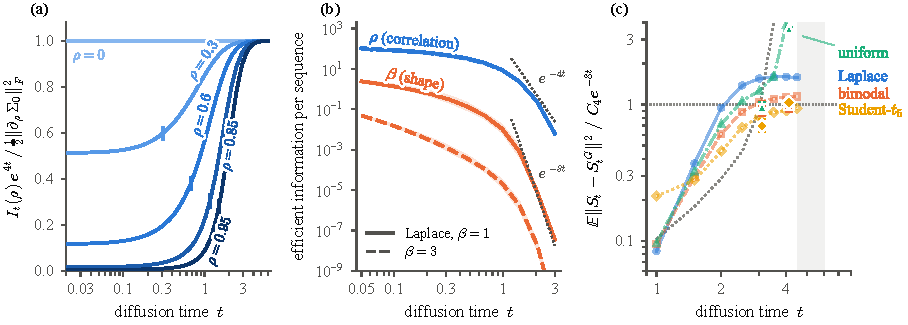
\includegraphics[width=\textwidth]{fig_theory.pdf}
\end{center}

\paragraph{Panel (a).} Horizontal axis: diffusion time $t$, logarithmic. Vertical
axis: the exact Fisher information of the Gaussian chain about $\corr$, divided by its
predicted asymptote $\tfrac12\Frob{\partial_\corr\Sig_0}^2e^{-4t}$, so that the theorem
predicts the value one (dotted line). One curve per correlation, in a blue ramp from
$\corr=0$ to $0.95$; the short vertical tick on each curve marks its crossover
$\tstar(\corr)=\tfrac12\log\lmax(\Sig_0)$. Reading: every curve rises to one, which is
the paper's Theorem~3 for a covariance coordinate, exactly (there is no Monte Carlo in
this panel; the information is the closed-form trace of
\Cref{ch:fisher-cramer-rao}); the more correlated the chain, the later the curve
arrives, and the tick shows that the arrival is governed by $\tstar$. At $\corr=0$ the
curve is one at every $t$. The curves are computed by the \code{gauss} part of E01.

\paragraph{Panel (b).} Both axes logarithmic: $t$ against the efficient Fisher information
per noised sequence, for the correlation coordinate $\corr$ (degree two, blue) and the
shape coordinate $\beta$ (degree four, orange) of the generalised-Gaussian chain, at the
Laplace member $\beta=1$ (solid) and at $\beta=3$ (dashed), estimated from
per-sequence scores obtained by Fisher's identity through the tree-exact recursion
(\Cref{ch:maximum-likelihood-em}); the bands are the range over eight replicates, and the
two dotted guides have slopes $-4$ and $-8$. Reading: above the crossover the two
families of curves run parallel to their guides, three decades apart, which is the
order-by-order decay; below it both are shallower, which is the pre-asymptotic regime.
The kinked Laplace density reaches the numerical floor of the outer-product estimate near
$t=2.5$, which is why the slopes quoted in the text are fitted on the smooth members.
The curves are the \code{shape} part of E01; the fitted slopes come from
\code{tools/make\_theory\_numbers.py}.

\paragraph{Panel (c).} Both axes logarithmic: $t$ from about one to five against the
measured closure gap $\E\lVert\score-\Sgauss\rVert^2$ divided by its predicted
value $\tfrac16\Frob{\kfour}^2e^{-8t}$, so that the theorem predicts one (dotted line).
Four innovation families (Laplace, bimodal, uniform, Student-$t_5$) from E18 on the wide
$(3201,32)$ grid: thin curves with small markers are the ratio from $512$ sequences,
paired across levels by a common noise draw, so their \emph{shape} is precise while
their level carries a common sampling factor; the bold markers with bars at $t=3$ and
$4$ are the constant from many more sequences with a chain bootstrap interval, and they
are what pins the level. The grey dotted curve is the same Student-$t_5$ sequences on the
operating $(801,8)$ domain, where the truncated prior drives the reference; the shaded
region beyond $t=4.5$ is where the double-precision floor of the posterior means enters.
Reading: every family reaches one within its interval, Student-$t_5$ included; the
departure of the grey curve is a truncation artefact, not the moment condition; the
uniform family, with the smallest constant, hits the floor first. Sources: E18 (the
\code{chain} and \code{constant} parts) and the E01 protocol; drawn by
\code{tools/make\_fig\_theory.py}.

\paragraph{Claims supported.} The rates $e^{-4t}$ and $e^{-8t}$, the constants
$\tfrac12\Frob{\partial_\corr\Sig_0}^2$ and $\tfrac16\Frob{\kfour}^2$, the crossover, and
the heavy-tailed regime as a statement about expectations rather than samples
(\Cref{ch:attenuation-theorems}).

\section{Figure 3: learning through noise (\code{fig\_learning.pdf})}
\label{sec:fig-learning}

\begin{center}
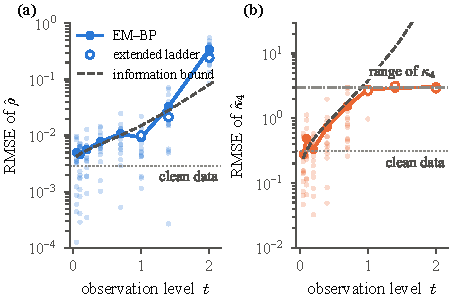
\includegraphics[width=\textwidth]{fig_learning.pdf}
\end{center}

\paragraph{What is plotted.} Two panels with a linear horizontal axis, the observation
level $t$ at which all $\nseq=512$ training sequences were noised, and a logarithmic
vertical axis. Panel (a): the error of the fitted correlation $\hat\corr$; panel (b):
the error of the fitted innovation excess kurtosis $\hat\kfour$. In each, faint points
are the sixteen individual fits $|\hat\theta-\theta|$ at that level, the solid line is
their RMSE, the dashed line is the Cram\'er--Rao reference $1/\sqrt{\nseq I_t}$ read from
the frozen E01 efficient information at the Laplace member (through the chain rule for
the kurtosis), the dotted horizontal line is the clean-data fit (the optimiser's own
floor at $t=0$), and in panel (b) the dash-dotted horizontal line at $3$ is the full range
of the coordinate, the distance from a Gaussian innovation to the truth. In the current
draft hollow markers add the same fits with the EM ladder extended (E06c), the budget
control (\Cref{ch:model-selection}).

\paragraph{How to read it.} At the lowest levels the points cluster around the reference
in both panels: the estimator is unimodal and at the information reference while the
coordinate is identifiable. Moving right in panel (b), the cloud splits into a cluster
near the reference and a group of points at the range line: those are fits that
collapsed to a Gaussian innovation. Where the dashed reference crosses the range line,
the information runs out and every fit collapses; panel (a) shows the correlation
surviving to a higher level, and being lost only past the crossover. The vertical
distance between the solid line and the dashed line, in decades, is the estimator's
inefficiency; where the points sit \emph{below} the reference the estimator is biased
(shrunk by early stopping) and the reference, being for an unbiased estimator in a
one-parameter family, is a yardstick rather than a bound (\Cref{ch:em-through-noise}).

\paragraph{Claims and sources.} The per-level statements of the paper's Section~4 (at
the reference while identifiable; collapse where the reference crosses the range; the
correlation survives to the crossover; the two highest levels possibly budget-limited).
Source: E06 (and E06c), \code{outputs/E06/levels.csv}; drawn and its macros written by
\code{tools/make\_learning\_numbers.py}; the collapse fractions and dispersions of the
text are from \code{tools/make\_audit\_numbers.py}. The moment estimators of E19
(\Cref{ch:quasi-likelihood-moments}) are quoted in the text as the rate-correct
competitor and, in the audit's recommended redesign, would appear as a second pair of
curves.

\section{Figure 4: capacity across the family (\code{fig\_family.pdf})}
\label{sec:fig-family}

\begin{center}
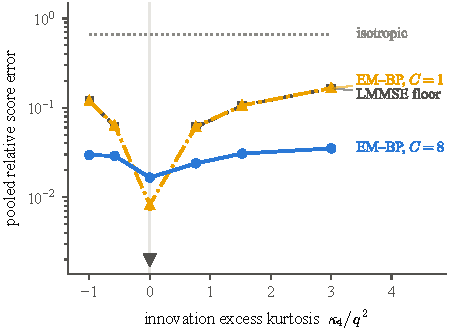
\includegraphics[width=\textwidth]{fig_family.pdf}
\end{center}

\paragraph{What is plotted.} Horizontal axis: the innovation's excess kurtosis
$\kfour/\ivar^2$, from $+3$ at the Laplace member through $0$ at the Gaussian member to
about $-1.1$ at the platykurtic end, along the generalised-Gaussian family at fixed
$\corr$ and variance; a vertical grid line marks zero. Vertical axis: pooled relative
score error, logarithmic. Four curves: the isotropic reference (grey dotted), the LMMSE
floor (dark dashed with hollow squares), EM--BP with a single Gaussian innovation
$\ncomp=1$ (dash-dotted triangles) and with $\ncomp=8$ (solid circles), the last two with
standard-error bars over sixteen seeds at $\nseq=512$. The floor is exactly zero at the
Gaussian member, which a logarithmic axis cannot show, so the dashed line is broken
there and a caret at the bottom marks the point.

\paragraph{How to read it.} The floor traces a V with its vertex at the Gaussian member:
that is the price of second-order closure across the family, largest where the fourth
cumulant is largest in either sign. The $\ncomp=1$ curve lies on the V within its bars
at every member, which is Proposition~1 read across a family
(\Cref{ch:gaussian-closure-lmmse,ch:quasi-likelihood-moments}). The $\ncomp=8$ curve
stays low throughout and meets the $\ncomp=1$ curve at the Gaussian member, where the
gap between them, the paired gain of capacity, is a small loss: with no fourth-order
structure to buy, the extra components only add variance.

\paragraph{Claims and sources.} Capacity buys exactly what closure discards; the gain is
ordered by $\kfour$; at the Gaussian member it reverses. Source: E02b,
\code{outputs/E02b/family.csv}; \code{tools/make\_family\_numbers.py}.

\section{Figure 5: where the structure stops helping (\code{fig\_misspec.pdf})}
\label{sec:fig-misspec}

\begin{center}
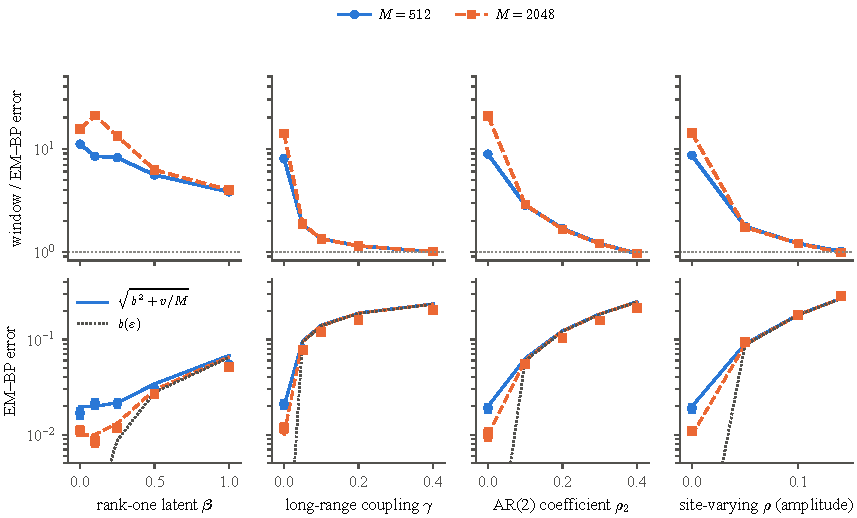
\includegraphics[width=\textwidth]{fig_misspec.pdf}
\end{center}

\paragraph{What is plotted.} Two rows of four panels, one column per misspecification
mechanism of \Cref{ch:misspecification-edgeworth}: the rank-one latent (strength
$\beta$), long-range precision coupling ($\gamma$), the AR(2) second coefficient
($\corr_2$) and the site-varying correlation (amplitude $\delta$). Top row: the ratio of
the radius-$2$ window head's error to EM--BP's, formed within seed and averaged,
against the strength, logarithmic vertical axis shared across the row, one curve per
sample size ($\nseq=512$ and $2048$; the legend is a single strip above the row); the
dotted horizontal line is ratio one. Bottom row: EM--BP's own error at both sizes
(points with paired standard errors), the closed-form bias $b(\varepsilon)$ of the
Kullback--Leibler projection (dark dotted) and the finite-sample prediction
$\sqrt{b(\varepsilon)^2+v/\nseq}$ for each size (lines), with $v$ read from the
well-specified cells.

\paragraph{How to read it.} In the top row, a curve above the dotted line means the
misspecified chain estimator still beats the network; where it crosses below, the
network wins. The crossing is reported as the two bracketing strengths, never as a
fitted point. A curve that stays above the line across the whole swept range (the
rank-one latent) is a mechanism this estimator absorbs; a curve that reaches the line
but does not cross it (long-range coupling, at the largest strength) is a tie. In the
bottom row the two sizes separate estimation from bias: at zero strength the points of
the two sizes are apart and the larger sample is lower (estimation); at large strength
they coincide on the dotted bias curve (bias that no sample size removes). The slope of
the bias curve at small strength on these axes is its order: linear for three mechanisms
and quadratic for the latent.

\paragraph{Claims and sources.} Graceful degradation; mechanism-dependent break-even;
the closed-form bias reproducing the large-sample error; the order in the strength
explaining which mechanisms bite. Sources: E08 (\code{outputs/E08/misspecification.csv})
for the points and ratios, E17 (\code{outputs/E17/bias.csv}) for the curves;
\code{tools/make\_misspec\_numbers.py}. The network arm is the radius-$2$, width-$64$
window head of \Cref{ch:neural-baselines}, not the screen's radius-$4$ winner.

\section{Figure 6: the floor across correlation (\code{fig\_phase.pdf})}
\label{sec:fig-phase}

\begin{center}
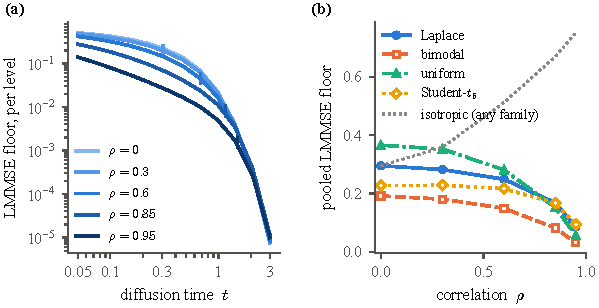
\includegraphics[width=\textwidth]{fig_phase.pdf}
\end{center}

\paragraph{What is plotted.} An appendix figure from the deterministic oracle ladder.
Panel (a): log--log axes, $t$ against the per-level LMMSE floor on the Laplace chain, one
curve per correlation in $\{0,0.3,0.6,0.85,0.95\}$ (blue ramp), with a tick at
$\tstar(\corr)$ on each. Panel (b): the schedule-pooled LMMSE floor against $\corr$
(linear horizontal axis) for the four non-Gaussian families, with the isotropic
reference as a grey dotted curve (the isotropic floor is the same for every family, so
one curve serves). In the current draft the Student-$t_5$ curve is computed on a wider
domain, where its $\corr=0$ cell is converged (E07b, E07c); earlier drafts ringed that
point as excluded.

\paragraph{How to read it.} In panel (a) each floor is flat at low $t$ and collapses after
its tick: past the crossover the twin's score is nearly the score, at every
correlation. In panel (b) the families are ordered by the size of their fourth
cumulant at every $\corr$ (Laplace above uniform above bimodal, with the heavy-tailed
family where its constant puts it), and every floor falls with $\corr$ while the
isotropic reference rises: a strongly correlated chain has a score dominated by its
second-order part, so closure costs relatively less and learning nothing costs more.

\paragraph{Claims and sources.} The floor is a function of the innovation law and of
$\corr$; the crossover locates its collapse; the ordering by $\kfour$. Source: E07 (and
E07b, E07c), \code{outputs/E07/ladder.csv}; \code{tools/make\_fig\_phase.py}, which also
writes the phase macros.

\section{Figure 7: locality against its floor (\code{fig\_locality.pdf})}
\label{sec:fig-locality}

\begin{center}
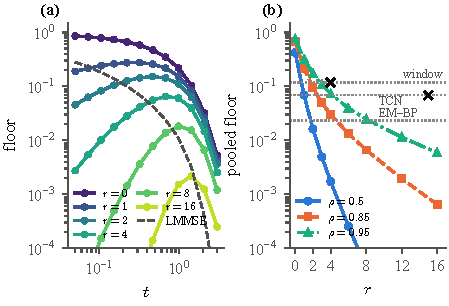
\includegraphics[width=\textwidth]{fig_locality.pdf}
\end{center}

\paragraph{What is plotted.} Panel (a): log--log axes, $t$ against the relative score
error of the best estimator that sees only the window $x_{i-r},\dots,x_{i+r}$ (the exact
posterior mean given the window, computed by sum-product on the sub-chain with the exact
marginal of the window's first site as initial factor), for radii $r\in\{0,1,2,4,8,16\}$
in a colour ramp, on the Laplace chain at $\corr=0.85$, with the Gaussian twin's full
LMMSE as a dashed line for scale. Panel (b): the same floor pooled over the schedule
against the radius, one curve per correlation in $\{0.5,0.85,0.95\}$; dotted horizontal
lines mark the frozen all-site errors at $\nseq=2048$ of the window head, the dilated
TCN and EM--BP, and crosses mark the two networks' radii.

\paragraph{How to read it.} In panel (a) the radius-zero curve is the price of using no
neighbours at all, and the curves fall quickly with $r$: at low noise one site is
nearly enough, at intermediate levels even a radius of sixteen leaves a small
remainder. In panel (b) the floor at the window head's radius is far below the head's
own error line: the plateau of the local architecture is not the information ceiling of
its radius but a limit of the architecture and its training. The gap between the floor
at $\corr=0.5$ and at $0.95$ shows that locality costs more when the chain is more
correlated, and that at $\corr=0.95$ the radius-four floor approaches the LMMSE floor
itself.

\paragraph{Claims and sources.} The withdrawal of ``locality is a ceiling'' and its
replacement by the floor; the non-Gaussian content of a wider window. Sources: E15
(\code{outputs/E15/locality.csv}) for the floors, E03 and E02a for the marks;
\code{tools/make\_fig\_locality.py}. One point to check against the paper: the
generator places the window head's cross at radius $2$ and the caption calls it the
radius-$2$ head, while the confirmatory head of E03, whose error the mark shows, has
radius $4$ (\code{outputs/E03/winners.json}); the text beside the figure compares that
error with the radius-$4$ floor.

\section{The tables}
\label{sec:tables}

\subsection{Table 1: capacity (\code{tab-capacity.tex})}

Rows: the LMMSE floor and EM--BP with $\ncomp\in\{1,2,4,8,16\}$. Columns: the four sample
sizes and a last column, $\nseq=\infty$, which is not a fit but the population reference
of E09: the $\ncomp$-component mixture innovation closest in Kullback--Leibler divergence
to the Laplace law, scored by tree-exact BP on the same test bundles. Entries are the
all-site pooled error averaged over sixteen seeds; standard errors, paired differences
and bootstrap intervals are in the macros and the text. A dagger marks a fit whose
narrowest component is under two grid cells, reported and not dropped. Reading: the
$\ncomp=1$ row equals the floor row to the printed precision at every size, which is the
apparatus check of \Cref{ch:quasi-likelihood-moments}; every $\ncomp\ge2$ row is far
below it; the best capacity moves right with the sample size; the $\infty$ column says
what each capacity could express with unlimited data, a reference and not a bound
(a Kullback--Leibler-optimal innovation need not minimise the score error). Sources:
E02a (\code{outputs/E02a/capacity.csv}) and E09 (\code{outputs/E09/floor.csv});
\code{tools/make\_capacity\_numbers.py}. The retired reading of the earlier capacity
study and its stopping-rule diagnosis are in the paper's appendix on capacity.

\subsection{Table 2: baselines under one recipe (\code{tab-baselines.tex})}

Rows: the four sample sizes. Columns: the isotropic reference, the LMMSE floor, the six
architectures (MLP, window head, TCN, bi-GRU, transformer, U-Net) under interface~A with
their screened configurations, and EM--BP with $\ncomp=8$. Entries: all-site pooled error,
mean over the sixteen confirmatory seeds, every arm on identical test bundles (the
oracles and EM--BP come from the capacity experiment and are joined on the bundle hash).
Reading: down a column, how each estimator improves with data; along a row, the ladder
isotropic, networks, floor, EM--BP, exact (zero). The fully connected network is far
behind the weight-shared ones at every size; the window head is the best network at the
smallest size and the worst of the shared five at the largest; several networks cross
the floor at $\nseq=2048$, so the floor is not a barrier for them; EM--BP is ahead
everywhere. The paired factors against EM--BP, the at-cap rates and the matched-interface
numbers are macros in the text. Source: E03 confirm (\code{outputs/E03/confirm.csv});
\code{tools/make\_baseline\_numbers.py}.

\subsection{Table 3: length extrapolation (\code{tab-length.tex})}

Rows: the five length-agnostic networks and EM--BP, all fitted at $\nsites=32$ and
$\nseq=2048$. Columns: the test length $\nsites\in\{32,64,128,256\}$, each scored against
the tree-exact score of chains of that length. Reading: a length-agnostic estimator
should improve slightly with length, because longer chains have proportionally fewer
boundary sites; EM--BP is flat, since inference at any length is the same exact recursion
with the same kernel; the convolutional and recurrent networks improve a little, the
window head most (its boundary error is a large share at $\nsites=32$); the transformer
degrades steeply, for the positional-encoding reason of \Cref{ch:neural-baselines}.
Sources: E03 length (\code{outputs/E03/length.csv}) and EM--BP re-evaluated at each
length by \code{tools/eval\_em\_length.py} (\code{outputs/E03/em\_length.csv});
\code{tools/make\_baseline\_numbers.py}.

\subsection{Table 4: generation (\code{tab-generation.tex})}

Rows, in two blocks for $\nseq\in\{128,2048\}$: the reference sample of the true law at
$t_{\min}$, then the samplers driven by the exact score, the fitted EM--BP kernel, the
LMMSE twin, the isotropic score, and two network checkpoints (bi-GRU, window head) from
E03. Columns: $\Delta\ell$, the mean log-likelihood gap in nats per sequence between the
generated sample and the reference sample under the true $P_{t_{\min}}$, computed by
the exact evidence of the tree-exact recursion (the exact arm's own gap is the sampler's
discretisation floor); $\hat\kfour$, the excess kurtosis of the innovations of the
generated chains; the lag fourth cumulant; and a sliced Wasserstein-2 distance. Every arm
integrates the same reverse SDE (\Cref{ch:reverse-sde-generation}) on the same Brownian
path within a seed, so the comparison is paired. Reading: the fitted kernel sits close to
the exact arm in $\Delta\ell$ and reproduces the innovation kurtosis; the twin generates a
Gaussian chain (kurtosis zero by construction) at a much larger gap; the isotropic score
is off by tens of nats; the Wasserstein column barely separates the arms, which is why
the likelihood gap is the headline. Source: E05 (\code{outputs/E05/generation.csv});
\code{tools/make\_generation\_numbers.py}.

\subsection{Table 5: the architecture screen (\code{tab-screen.tex})}

An appendix table. Rows: the six architecture families. Columns: the selected
configuration (hyperparameters, learning rate, parameterisation), its parameter count,
its pooled bulk risk on the development seeds, and the risk of the family's runner-up.
The caption's statement of the screen budget is generated from the screening file
itself (number of development seeds, restarts and steps found in it). Reading: the
screen ranks configurations within a family and never produces a headline; the
parameter counts are those derived by hand in \Cref{ch:neural-baselines}; a family
whose winner and runner-up are close was insensitive to the choice. Source: E03 screen
(\code{outputs/E03/screening.csv}); \code{tools/make\_baseline\_numbers.py}. A reader
comparing this caption with the paper's protocol appendix should note that the two
describe the screen budget differently (the appendix text gives the amended two-seed,
one-run, $16{,}000$-step budget; the generated caption reports what the frozen screening
file contains), and take the generated caption as the description of the file the
table was made from.

\subsection{Table 6: the oracle ladder}

An appendix table typed from macros: for each of five innovation families (Laplace,
Student-$t_5$, uniform, bimodal, Gaussian) its excess kurtosis and the pooled relative
score error of the isotropic score $-\vx$ and of the LMMSE oracle with the true
covariance, from $512$ chains at the frozen configuration. Reading: the isotropic column
is nearly the same for every family (it measures the covariance the estimator has not
learned, which every family shares); the LMMSE column is the exact price of second-order
closure per family, zero for the Gaussian, and the floor every second-order estimator is
bounded by. Source: \code{tools/make\_oracle\_numbers.py}, a deterministic computation
recorded in \code{docs/AUDIT\_ORACLE\_LADDER.md}; its values are cross-checked by the
oracle rows of the capacity experiment on the confirmatory bundles.

\subsection{Generated fragments the current body does not input}

The generator suite also emits a regime table (\code{regime-table.tex}, from E13; the
paper quotes its content as macros in the regime paragraph) and several tables of the
archival comparison (\code{tab-efficiency}, \code{tab-structured}, \code{tab-aggregation},
\code{tab-screening}, \code{tab-hellinger}, \code{tab-convergence}), which the manuscript
check regenerates for consistency but which the current body files do not include.
Likewise \code{paper/figures/} holds figures of the archival study (capacity,
screening, sample efficiency, value of structure, the non-Markov study, the grid domain
and the toy-model score) drawn by \code{tools/make\_figures.py} from the archival
outputs; they are not referenced by the current manuscript and are not discussed here.

\where{\begingroup\sloppy Every figure environment and \code{\textbackslash input} of a
table in \code{paper/body/*.tex}; the captions quoted above. Generators:
\code{tools/make\_fig\_theory.py}, \code{tools/make\_learning\_numbers.py},
\code{tools/make\_family\_numbers.py}, \code{tools/make\_misspec\_numbers.py},
\code{tools/make\_fig\_phase.py}, \code{tools/make\_fig\_locality.py},
\code{tools/make\_capacity\_numbers.py}, \code{tools/make\_baseline\_numbers.py},
\code{tools/make\_generation\_numbers.py}, \code{tools/make\_oracle\_numbers.py},
\code{tools/make\_regime\_numbers.py}, \code{tools/figstyle.py};
\code{paper/figures/fig\_mechanism.tex}; \code{docs/FIGURE\_TABLE\_STANDARDS.md}.
Experiments: E01, E02a, E02b, E03, E05, E06, E06c, E07, E07b, E07c, E08, E09, E13, E15,
E17, E18.\par\endgroup}

\paragraph{References.}
\begingroup\sloppy
E.~R.~Tufte, 2001, \emph{The Visual Display of Quantitative Information}, second edition, Graphics Press.
W.~S.~Cleveland, 1993, \emph{Visualizing Data}, Hobart Press.
J.~D.~Hunter, 2007, Matplotlib: a 2D graphics environment, \emph{Computing in Science and Engineering} 9, 90--95.
T.~Tantau, 2023, \emph{The TikZ and PGF Packages}, manual for version 3.1.10.\par\endgroup
\endgroup


\appendix
\chapter{Glossary}
\label{ch:glossary}

Every technical term used in the paper and in this compendium, in alphabetical order,
with one to three sentences and the chapter in which it is defined. Symbols follow the
paper's notation (\Cref{ch:conventions}).

\begingroup\sloppy
\begin{description}[leftmargin=1.6em,itemsep=0.25em,font=\normalfont\bfseries]

\item[Adam] A first-order stochastic optimiser that scales each parameter's update by
running estimates of the gradient's mean and magnitude; the optimiser of every network
arm. \Cref{ch:neural-baselines}.

\item[Affine layer] A map $\vect{h}\mapsto\mat{W}\vect{h}+\vect{b}$; the basic block of every
network, with $mn+m$ parameters for an $m\times n$ weight. \Cref{ch:neural-baselines}.

\item[Amendment, pre-data] A dated entry in a registry file recording a change to a
registered design or analysis made before any confirmatory cell has produced a number;
the instrument by which a registration is corrected without losing its guarantee.
\Cref{ch:protocol}.

\item[Amplitude (of a feature)] The size of a Hermite moment of degree $m$, attenuated by
the channel as $e^{-mt}$; the first of the three clocks. \Cref{ch:attenuation-theorems}.

\item[AR(1) chain] A first-order autoregression $a_i=\corr a_{i-1}+\varepsilon_i$ with
i.i.d.\ innovations; the paper's data model, with $a_1\sim\normal01$ and
$\ivar=1-\corr^2$. \Cref{ch:markov-chains}.

\item[AR(2)] A second-order autoregression $a_i=\corr_1a_{i-1}+\corr_2a_{i-2}+\varepsilon_i$;
one of the four misspecification mechanisms, parameterised by $\corr_2$ at fixed lag-one
correlation. \Cref{ch:misspecification-edgeworth}.

\item[Assumption (exponential moment)] $\E e^{\lambda|\va|}<\infty$ for some $\lambda>0$,
the hypothesis of the paper's Theorem~3; every family used except Student-$t$ satisfies
it. \Cref{ch:attenuation-theorems}.

\item[Asymptotic relative efficiency] The limiting ratio of the Cram\'er--Rao variance to
an estimator's variance; one for an efficient estimator, below one otherwise.
\Cref{ch:quasi-likelihood-moments}.

\item[At cap] A cell whose validation-selected checkpoint is the last rung of its ladder,
so the reported error is an upper bound on what a longer ladder would give.
\Cref{ch:model-selection}.

\item[Attention (self-attention)] The transformer's operation in which every site forms a
softmax-weighted average of every other site's representation with weights it computes
from the data. \Cref{ch:neural-baselines}.

\item[Attenuation, Hermite] The exact identity $\E_{\Pt}[H_\nu(\vx_t)]=e^{-|\nu|t}\E_{\Pz}[H_\nu(\va)]$,
the paper's Theorem~2. \Cref{ch:attenuation-theorems}.

\item[Audit script] \code{tools/audit\_claims.py}, an independent recomputation of every
headline number from the frozen CSVs with plain code, compared with the macros.
\Cref{ch:protocol}.

\item[Backward message] $\rmsg_i$, the function of $a_i$ carrying the evidence from sites
$i+1,\dots,\nsites$; the right-to-left sweep of sum-product. \Cref{ch:factor-graphs-bp}.

\item[Belief (site marginal)] The posterior density of one site,
$\propto\lmsg_i\like\rmsg_i$; its mean is $\pmeansite{i}$. \Cref{ch:factor-graphs-bp}.

\item[Belief propagation] Sum-product message passing on a factor graph; exact on a tree,
hence exact for the paper's posterior. \Cref{ch:factor-graphs-bp}.

\item[Bias (of an estimator)] $\E\hat\theta-\theta$; in misspecification, the error that
remains as $\nseq\to\infty$. \Cref{ch:fisher-cramer-rao,ch:misspecification-edgeworth}.

\item[Bi-GRU] A bidirectional gated recurrent network; one of the six baselines.
\Cref{ch:neural-baselines}.

\item[Bimodal innovation] The symmetric two-component Gaussian mixture innovation (separation
parameter $0.6$), excess kurtosis $-0.72$. \Cref{ch:markov-chains}.

\item[Bootstrap, percentile] Resampling seeds with replacement and reporting the $2.5$th
and $97.5$th percentiles of the resampled statistic; the paper's interval for paired
ratios. \Cref{ch:experimental-statistics}.

\item[Break-even] The misspecification strength at which the paired log-ratio of the
network's error to EM--BP's changes sign; reported as the bracketing grid points.
\Cref{ch:misspecification-edgeworth}.

\item[Bulk region] Sites $5$ to $\nsites-4$; the region used for checkpoint selection.
\Cref{ch:model-selection}.

\item[Bundle] A fixed set of chains with their noised views at every level and the
reference posterior means under the true kernel; training, validation and test bundles
are drawn from disjoint keyed streams. \Cref{ch:model-selection}.

\item[Capacity (mixture)] The number of components $\ncomp$ of the mixture-innovation
kernel. \Cref{ch:em-through-noise}.

\item[Cell] One unit of work of a driver (one seed at one size, say), written to its own
file so that a run is resumable. \Cref{ch:protocol}.

\item[Checkpoint ladder] The fixed list of budgets (EM iterations or gradient steps) at
which a fit is saved; the selected checkpoint is chosen afterwards among its rungs.
\Cref{ch:model-selection}.

\item[Clean chain] The unnoised sequence $\va\sim\Pz$. \Cref{ch:conventions}.

\item[Closure gap] $\E_{\Pt}\lVert\score-\Sgauss\rVert^2$, the squared distance between
the true score and the covariance twin's; $\tfrac16\Frob{\kfour}^2e^{-8t}$ to leading order.
\Cref{ch:attenuation-theorems}.

\item[Coloured probes] The $2r+1$ deterministic probe vectors that give the exact trace of
a Jacobian of bandwidth $r$; the divergence estimator of the window head.
\Cref{ch:neural-baselines}.

\item[Common random numbers] Keying every random stream by a tag so that compared arms see
the same draws and their difference is not Monte Carlo noise. \Cref{ch:protocol}.

\item[Conditional expectation] $\E[Y\mid X]$, the best mean-square predictor of $Y$ from
$X$; the posterior mean is the case $Y=\va$, $X=\vx_t$. \Cref{ch:conventions}.

\item[Confirmatory seeds] Seeds $0$--$15$ (eight in the sweeps), used only for reported
numbers, never for selection. \Cref{ch:model-selection}.

\item[Consistency] Convergence of an estimator to the true (or pseudo-true) parameter as
$\nseq\to\infty$. \Cref{ch:fisher-cramer-rao,ch:quasi-likelihood-moments}.

\item[Convolution, one-dimensional] A weight-shared linear map of a signal whose output
at $i$ depends on inputs within a fixed radius; zero-padded at the ends.
\Cref{ch:neural-baselines}.

\item[Correlation coordinate] A parameter that moves the covariance $\Sig_0$, such as
$\corr$; a degree-two coordinate. \Cref{ch:attenuation-theorems}.

\item[Covariance twin] The Gaussian chain with the same $\corr$ and $\ivar$; its score is
$\Sgauss=-\Sig_t^{-1}\vx$. \Cref{ch:gaussian-closure-lmmse}.

\item[Cram\'er--Rao bound] $\Var\hat\theta\ge1/(\nseq I(\theta))$ for an unbiased estimator;
the reference curve of the learning figure. \Cref{ch:fisher-cramer-rao}.

\item[Crossover time] $\tstar=\tfrac12\log\lmax(\Sig_0)$, where $e^{2t}$ passes the
largest eigenvalue of the clean covariance; the scale beyond which the asymptotic rates
apply. \Cref{ch:attenuation-theorems}.

\item[Cumulant] The coefficients of the log of the moment generating function; additive
over independent summands and homogeneous of degree $n$. \Cref{ch:moments-cumulants}.

\item[Cumulant generating function] $\log\E e^{s\cdot\va}$, whose Taylor coefficients are
the joint cumulants. \Cref{ch:moments-cumulants}.

\item[Damped cumulant generating function] $\Lambda(s,b)=\log\E_{\Pz}\exp(s\cdot\va-b|\va|^2/2)$,
the function whose grading gives the paper's Theorem~3. \Cref{ch:attenuation-theorems}.

\item[Delta method] The first-order propagation of an estimator's variance through a
smooth function. \Cref{ch:experimental-statistics}.

\item[Denoiser] A map from a noised sequence and a level to an estimate of the posterior
mean; every network arm is one. \Cref{ch:neural-baselines}.

\item[Denoising score matching] Regressing the network on the clean chain (or the noise)
with fresh corruptions; its minimiser is the posterior mean, hence the score.
\Cref{ch:score-matching,ch:neural-baselines}.

\item[Development seeds] Seeds $10000$--$10003$, used only for architecture and
hyperparameter choices. \Cref{ch:model-selection}.

\item[Dilation] The spacing $d$ between the taps of a convolution; a dilated stack widens
its receptive radius by $d$ per layer. \Cref{ch:neural-baselines}.

\item[Divergence] $\nabla\cdot s=\sum_i\partial s_i/\partial x_i$, the trace of the score
map's Jacobian; the term implicit score matching must estimate. \Cref{ch:neural-baselines}.

\item[Drift (grid)] The relative change of the posterior-mean field between two grids on
the same chains; the quadrature convergence diagnostic. \Cref{ch:grid-quadrature}.

\item[Edgeworth correction] The expansion of a law around its covariance-matched Gaussian,
whose first term is $\tfrac1{24}\kfour$ contracted with the multivariate Hermite
polynomials. \Cref{ch:misspecification-edgeworth}.

\item[Efficient information] The Fisher information of a coordinate after the nuisance
coordinates are projected out. \Cref{ch:fisher-cramer-rao}.

\item[EM (expectation--maximisation)] Alternating an E-step (posterior expectations under
the current parameters) and an M-step (maximisation of the expected complete-data
log-likelihood). \Cref{ch:maximum-likelihood-em}.

\item[EM--BP] The paper's structured estimator: EM whose E-step is the tree-exact
recursion on the grid and whose kernel is the mixture-innovation AR(1) kernel.
\Cref{ch:em-through-noise}.

\item[Eps parameterisation] The network predicts the standardised noise $\vz$; the mean
is $(\vx-\sqrt{\Dt}\hat\varepsilon)/e^{-t}$. \Cref{ch:neural-baselines}.

\item[Estimand] The quantity a number estimates; the paper's is the schedule-pooled
relative score error. \Cref{ch:experimental-statistics}.

\item[Evidence (marginal likelihood)] $\Pt(\vx)$, the probability of the noised view under
the model, returned by the forward sweep with its constants accumulated.
\Cref{ch:grid-quadrature}.

\item[Evidence rule] Selecting EM's rung by the held-out one-view log-evidence per edge;
the oracle-free rule of E20 and E14. \Cref{ch:model-selection}.

\item[Exceedance count] The expected number of sites of a bundle beyond the grid domain,
$\nseq\nsites P(|a|>\halfwidth)$; the right diagnostic for polynomial tails.
\Cref{ch:grid-quadrature}.

\item[Excess kurtosis] $\kfour/\ivar^2$, the fourth cumulant divided by the squared variance;
$+3$ for Laplace, $0$ for Gaussian. \Cref{ch:moments-cumulants}.

\item[Factor graph] A bipartite graph of variables and factors representing a product
density; the posterior's is the prior's chain. \Cref{ch:factor-graphs-bp}.

\item[Fair screen] A screen in which every candidate is trained under the same recipe,
budget, bundles, ladder and selection rule on development seeds disjoint from the
confirmatory ones. \Cref{ch:model-selection}.

\item[Fisher divergence] $\tfrac12\E_p\lVert s_\theta-s_p\rVert^2$, what score matching
minimises. \Cref{ch:score-matching,ch:model-selection}.

\item[Fisher information] $I(\theta)=\E[(\partial_\theta\log P)^2]$; per noised sequence,
$I_t(\theta)$. \Cref{ch:fisher-cramer-rao}.

\item[Fisher's identity] The gradient of the marginal log-likelihood equals the posterior
expectation of the complete-data score; on the grid it is read off the pairwise
marginals. \Cref{ch:maximum-likelihood-em}.

\item[Forward message] $\lmsg_i$, the function of $a_i$ carrying the evidence from sites
$1,\dots,i-1$. \Cref{ch:factor-graphs-bp}.

\item[Forward process] The Ornstein--Uhlenbeck noising $\vx_t=e^{-t}\va+\sqrt{\Dt}\vz$.
\Cref{ch:ou-channel-tweedie}.

\item[Fourier features] The vector $(\log t,\sin2^k\log t,\cos2^k\log t)_{k\le3}$ by which the
level enters every network. \Cref{ch:neural-baselines}.

\item[Frobenius norm] $\Frob{\mat{A}}^2=\sum A_{ij}^2$, extended to tensors over ordered
index tuples. \Cref{ch:conventions}.

\item[Frozen configuration] \code{FROZEN}, the world every experiment runs in: chain,
channel, grid, schedule, seeds. \Cref{ch:protocol}.

\item[Frozen output] An output directory whose files are hashed into its registry entry;
immutable thereafter. \Cref{ch:protocol}.

\item[Gaussian closure] Moment-projected sum-product, which replaces every message by the
Gaussian with its mean and variance; equals the LMMSE of the covariance twin.
\Cref{ch:gaussian-closure-lmmse}.

\item[Gaussian quasi-likelihood] The Gaussian log-likelihood written for data that are
not Gaussian; depends on the data only through the sample covariance.
\Cref{ch:quasi-likelihood-moments}.

\item[GELU] The activation $x\Phi(x)$, a smooth rectifier. \Cref{ch:neural-baselines}.

\item[Generalised EM] An EM whose M-step only increases the expected complete-data
log-likelihood (conditional maximisation); its ascent is monotone.
\Cref{ch:maximum-likelihood-em}.

\item[Generalised Gaussian family] Innovations $\propto\exp(-|\varepsilon/s_\beta|^\beta)$
at fixed variance, from Laplace ($\beta=1$) through Gaussian ($\beta=2$) to platykurtic
members. \Cref{ch:markov-chains}.

\item[Generator] A script under \code{tools/} that reads frozen outputs and writes the
macros, tables and figures of the paper. \Cref{ch:protocol}.

\item[Gradient clipping] Rescaling the gradient to a maximum norm before an optimiser
step; at $1$ in the recipe. \Cref{ch:neural-baselines}.

\item[Grid (quadrature)] The $\ngrid$ uniform points on $[-\halfwidth,\halfwidth]$ on which
messages are carried with trapezoidal weights. \Cref{ch:grid-quadrature}.

\item[GRU] Gated recurrent unit; a recurrence with reset and update gates.
\Cref{ch:neural-baselines}.

\item[H\'ajek--Le Cam] The local asymptotic minimax theorem: no estimator beats
$1/I^{\mathrm{eff}}$ locally, and maximum likelihood attains it.
\Cref{ch:fisher-cramer-rao}.

\item[Heavy tails] Innovation laws with polynomial tails (Student-$t$), outside the
exponential-moment assumption, with an $e^{-\nu t}$ term in the expected gap.
\Cref{ch:attenuation-theorems}.

\item[Held-out] Data not used to fit; the validation bundle for selection, the test
bundle for scoring. \Cref{ch:model-selection}.

\item[Hermite moment] $\E[H_\nu(\vx)]$ with $H_\nu$ a product of Hermite polynomials over
sites; the quantity the channel attenuates diagonally. \Cref{ch:gaussian-hermite}.

\item[Hermite polynomial] The probabilists' $\Hen{n}$, orthogonal under the standard
Gaussian with $\E\Hen{n}^2=n!$. \Cref{ch:gaussian-hermite}.

\item[Hutchinson's estimator] $\vect{v}^\top\mat{J}\vect{v}$ with a standard normal probe,
an unbiased but noisy estimate of $\tr\mat{J}$. \Cref{ch:neural-baselines}.

\item[Hyv\"arinen identity] $\E_p[\tfrac12\lVert s\rVert^2+\nabla\cdot s]=\tfrac12\E_p\lVert s-s_p\rVert^2+\text{const}$,
by integration by parts. \Cref{ch:score-matching,ch:model-selection}.

\item[Identifiability] Distinct parameters give distinct laws; $(\corr,\ivar)$ is
identifiable from $\Sig_0$, hence from the noised covariance.
\Cref{ch:quasi-likelihood-moments}.

\item[Implicit score matching] Minimising Hyv\"arinen's objective on noisy samples only;
the loss of interface~C. \Cref{ch:score-matching,ch:neural-baselines}.

\item[Information interface] What a learner may see: A (clean chains, fresh corruptions),
B (clean chains, one fixed corruption), C (one noised view per sequence and nothing
else). \Cref{ch:model-selection}.

\item[Innovation] The i.i.d.\ increment $\varepsilon_i$ of the chain, with density $\innov$
of mean zero and variance $\ivar$. \Cref{ch:markov-chains}.

\item[Isotropic score] $-\vx$, the score of $\normal0{\Id}$; the reference of a model that
learned nothing beyond the unit variance. \Cref{ch:gaussian-closure-lmmse}.

\item[Isserlis' theorem] Gaussian moments are sums over pairings of covariances (also
Wick's theorem). \Cref{ch:gaussian-hermite}.

\item[k-statistic] Fisher's exactly unbiased sample cumulant. \Cref{ch:quasi-likelihood-moments}.

\item[Kalman smoother] The linear-Gaussian smoother; the Gaussian part of the paper's
score. \Cref{ch:gaussian-closure-lmmse}.

\item[Kernel (transition)] $\kernel(a'\mid a)=\innov(a'-\corr a)$; $\kernelth$ when
parameterised. \Cref{ch:markov-chains}.

\item[Kullback--Leibler divergence] $\KL(p\|q)=\E_p\log(p/q)\ge0$, zero only at $p=q$.
\Cref{ch:conventions}.

\item[Kullback--Leibler projection] The member of a family closest to a law in
$\KL(\text{law}\|\cdot)$; the limit of a misspecified maximum-likelihood estimator.
\Cref{ch:misspecification-edgeworth}.

\item[Lag-one moment estimator] $\hat\corr=e^{2t}\,\overline{x_ix_{i+1}}$, unbiased for
$\corr$ by Hermite attenuation. \Cref{ch:quasi-likelihood-moments}.

\item[Laplace innovation] The double-exponential density, excess kurtosis $3$; the
frozen family. \Cref{ch:markov-chains}.

\item[Layer normalisation] Rescaling a representation to zero mean and unit variance
across channels with a learned gain and shift. \Cref{ch:neural-baselines}.

\item[Length-agnostic] An architecture that refers to no fixed $\nsites$ and can be
applied at any length. \Cref{ch:neural-baselines}.

\item[LMMSE] The linear minimum-mean-square estimator $e^{-t}\Sig_0\Sig_t^{-1}\vx$ of
$\va$ from $\vx_t$; the best linear map. \Cref{ch:gaussian-closure-lmmse}.

\item[LMMSE floor] The relative score error of the LMMSE with the true covariance; the
bound of every second-order estimator. \Cref{ch:gaussian-closure-lmmse}.

\item[Locality floor] The error of the best estimator that sees only a window of radius
$r$, the exact posterior mean given the window. \Cref{ch:attenuation-theorems}.

\item[Log-evidence per edge] The held-out marginal log-likelihood divided by the number
of transitions; the evidence rule's statistic. \Cref{ch:model-selection}.

\item[Log-spaced schedule] The twelve levels $0.05\cdot60^{(k-1)/11}$. \Cref{ch:protocol}.

\item[M-estimator] The solution of an estimating equation $\sum_\mu\psi(\vx^\mu;\theta)=0$;
its variance is the sandwich. \Cref{ch:quasi-likelihood-moments}.

\item[M-step] The maximisation step of EM; for a Gaussian kernel the belief-weighted
Yule--Walker pair. \Cref{ch:maximum-likelihood-em}.

\item[Marginal likelihood] See evidence. \Cref{ch:maximum-likelihood-em}.

\item[Markov chain] A sequence in which each site depends on the past only through its
predecessor. \Cref{ch:markov-chains}.

\item[Matched interface] Interface~C, EM--BP's own; the comparison at matched information.
\Cref{ch:model-selection}.

\item[Mehler's identity] $\E_z\Hen{n}(\alpha a+\sqrt{1-\alpha^2}z)=\alpha^n\Hen{n}(a)$; the
proof of Hermite attenuation. \Cref{ch:gaussian-hermite}.

\item[Method of moments] Solving sample moments equal to model moments for the parameter.
\Cref{ch:quasi-likelihood-moments}.

\item[Misspecification] Fitting a family that does not contain the truth.
\Cref{ch:misspecification-edgeworth}.

\item[Mixture-innovation kernel] $\kernelth(a'\mid a)=\sum_c\pi_c\normal{a'-\corr a-\nu_c}{s_c^2}$,
the paper's parametric kernel. \Cref{ch:em-through-noise}.

\item[MLP] The fully connected network; the baseline with no weight sharing.
\Cref{ch:neural-baselines}.

\item[Moment] $\E[X^n]$ or its multivariate version. \Cref{ch:moments-cumulants}.

\item[Multi-index] $\nu\in\mathbb N^{\nsites}$ with $|\nu|=\sum\nu_i$, labelling a product
of Hermite polynomials. \Cref{ch:gaussian-hermite}.

\item[Multivariate Hermite polynomial] $H^\Sig_{ijkl}=\partial_i\partial_j\partial_k\partial_l\phi_\Sig/\phi_\Sig$,
the tensor version of $\Hen{4}$ for a Gaussian with covariance $\Sig$.
\Cref{ch:misspecification-edgeworth}.

\item[Noised view] One draw $\vx=e^{-t}\va+\sqrt{\Dt}\vz$ at one level.
\Cref{ch:ou-channel-tweedie}.

\item[One-view protocol] Each training sequence contributes one noised view at one level,
the sequences split evenly across the twelve levels. \Cref{ch:em-through-noise}.

\item[Oracle] A quantity that uses the truth (the true kernel's posterior means, the true
score); an oracle rule is a selection rule that uses one. \Cref{ch:model-selection}.

\item[Oracle selection rule] Choosing the rung by the validation risk against the true
kernel's posterior means on the bulk. \Cref{ch:model-selection}.

\item[Ornstein--Uhlenbeck channel] The coordinatewise noising process with decay $e^{-t}$
and variance $\Dt=1-e^{-2t}$, which keeps the unit variance. \Cref{ch:ou-channel-tweedie}.

\item[Outer-product information estimate] Estimating Fisher information by the sample
covariance of per-sequence scores. \Cref{ch:fisher-cramer-rao}.

\item[Overfull box] A line LaTeX could not fit in its width; a gate of the manuscript
check for tables and figures. \Cref{ch:protocol}.

\item[Paired comparison] A difference or ratio formed within seed on identical bundles
before averaging over seeds. \Cref{ch:experimental-statistics}.

\item[Parameter count] The number of trainable numbers of a network, fixed by its
architecture. \Cref{ch:neural-baselines}.

\item[Pointwise MLP] Affine maps and activations applied at each site separately
(width-one convolutions). \Cref{ch:neural-baselines}.

\item[Pooled relative score error] $\bigl(\sum_t\sum_{j,i}(\hat s-s)^2/\sum_t\sum_{j,i}s^2\bigr)^{1/2}$,
the paper's estimand. \Cref{ch:experimental-statistics}.

\item[Posterior mean] $\pmean{\va}=\E[\va\mid\vx_t=\vx]$; the score is
$-(\vx-e^{-t}\pmean{\va})/\Dt$. \Cref{ch:ou-channel-tweedie}.

\item[Pre-registration] Writing hypothesis, design, seeds and analysis before the data
exist. \Cref{ch:protocol}.

\item[Provenance record] \code{params\_<part>.json}: commit, dirty list, archive digest,
host, resolved settings. \Cref{ch:protocol}.

\item[Pseudo-true parameter] The minimiser of $\KL(P^\star\|Q_\theta)$; where a
misspecified estimator converges. \Cref{ch:misspecification-edgeworth}.

\item[Quadrature, trapezoidal] Approximating an integral by a weighted sum on a uniform
grid; second order in the spacing for smooth integrands. \Cref{ch:grid-quadrature}.

\item[Quasi-MLE] The maximiser of a quasi-likelihood; consistent for $(\corr,\ivar)$ here.
\Cref{ch:quasi-likelihood-moments}.

\item[Quasi-score] The derivative of the quasi-likelihood; a moment equation in the
sample covariance. \Cref{ch:quasi-likelihood-moments}.

\item[Receptive radius] The $r$ such that a network's output at site $i$ depends on inputs
within $|j-i|\le r$ only. \Cref{ch:neural-baselines}.

\item[Registry] \code{experiments/registry/<id>.json}: hypothesis, design, analysis, seeds,
status, amendments, frozen digests. \Cref{ch:protocol}.

\item[Relative-position bias] A learned attention bias depending on the clipped offset
$i-j$; what makes the transformer length-agnostic. \Cref{ch:neural-baselines}.

\item[Residual connection] $\vect{h}\mapsto\vect{h}+g(\vect{h})$. \Cref{ch:neural-baselines}.

\item[Reverse SDE] The time-reversed diffusion driven by the score, used to generate
samples. \Cref{ch:reverse-sde-generation}.

\item[RMSE] Root mean squared error over seeds of a fitted coordinate.
\Cref{ch:experimental-statistics}.

\item[Rung] One entry of a checkpoint ladder. \Cref{ch:model-selection}.

\item[Sample covariance] $\mat{S}=\nseq^{-1}\sum_\mu\vx^\mu\vx^{\mu\top}$.
\Cref{ch:quasi-likelihood-moments}.

\item[Sandwich covariance] $\mat{J}^{-1}\mat{V}\mat{J}^{-1}$, the asymptotic variance of an
M-estimator under a possibly wrong model. \Cref{ch:quasi-likelihood-moments}.

\item[Schedule] The twelve levels over which errors are pooled. \Cref{ch:protocol}.

\item[Score] $\score(\vx,t)=\nabla_{\vx}\log\Pt(\vx)$. \Cref{ch:ou-channel-tweedie}.

\item[Score matching] Fitting a score by minimising the Fisher divergence, implicitly or
by denoising. \Cref{ch:score-matching}.

\item[Screen] The selection of a configuration per architecture family on development
seeds. \Cref{ch:model-selection}.

\item[Seed] The integer that determines a random stream; the inferential unit of the
paper's comparisons. \Cref{ch:experimental-statistics}.

\item[SHA-256] A cryptographic hash producing a $256$-bit digest; a changed byte changes
the digest. \Cref{ch:protocol}.

\item[Shape coordinate] A parameter that leaves $\Sig_0$ fixed and moves $\kfour$; a
degree-four coordinate, such as the generalised-Gaussian exponent at fixed variance.
\Cref{ch:attenuation-theorems}.

\item[Site] One coordinate $i$ of the chain. \Cref{ch:conventions}.

\item[Sliced Wasserstein distance] A distance between samples averaged over random
one-dimensional projections; a column of the generation table.
\Cref{ch:reverse-sde-generation}.

\item[SLURM] The cluster scheduler that runs the registered experiments. \Cref{ch:protocol}.

\item[Sub-chain] A window of consecutive sites treated as a chain with the exact marginal
of its first site as initial factor; the locality floor's computation.
\Cref{ch:attenuation-theorems}.

\item[Sum-product] The message-passing algorithm computing marginals on a factor graph.
\Cref{ch:factor-graphs-bp}.

\item[TCN] The dilated temporal convolutional network, receptive radius $15$.
\Cref{ch:neural-baselines}.

\item[Test bundle] The $2048$ held-out chains on which a selected fit is scored.
\Cref{ch:model-selection}.

\item[Three clocks] Amplitude $e^{-mt}$, information $e^{-2mt}$, samples $e^{2mt}$ for a
feature first visible at Hermite degree $m$. \Cref{ch:attenuation-theorems}.

\item[Time features] See Fourier features. \Cref{ch:neural-baselines}.

\item[Transformer] The attention-based encoder with relative-position bias.
\Cref{ch:neural-baselines}.

\item[Truncation (domain)] The error from carrying messages on a finite domain; bounded
by the exceedance count, not by the grid spacing. \Cref{ch:grid-quadrature}.

\item[Tweedie's identity] $\score(\vx,t)=-(\vx-e^{-t}\pmean{\va})/\Dt$.
\Cref{ch:ou-channel-tweedie}.

\item[Typed literal] A decimal typed into the manuscript rather than emitted by a
generator; forbidden unless listed with a justification. \Cref{ch:protocol}.

\item[U-Net] The two-resolution convolutional network with a skip connection.
\Cref{ch:neural-baselines}.

\item[Unary factor] $\like(x_i\mid a_i)\propto\exp[-(x_i-e^{-t}a_i)^2/2\Dt]$, the
likelihood factor attached to each site. \Cref{ch:factor-graphs-bp}.

\item[Uniform innovation] The uniform density at unit variance, excess kurtosis $-1.2$.
\Cref{ch:markov-chains}.

\item[Validation bundle] The $1024$ held-out chains on which the checkpoint is chosen.
\Cref{ch:model-selection}.

\item[Validation risk] The pooled relative score error on the validation bundle's bulk
against the true kernel's posterior means. \Cref{ch:model-selection}.

\item[Variance-matched family] Innovation laws with the same mean and variance, hence the
same $\Sig_0$, differing only beyond second order. \Cref{ch:markov-chains}.

\item[Weight sharing] Using the same parameters at every site, as a convolution or a
recurrence does. \Cref{ch:neural-baselines}.

\item[Wick product] ${:}x_ix_jx_k{:}$, the Hermite (orthogonalised) monomial; Wick's
theorem gives its Gaussian second moments by pairings. \Cref{ch:gaussian-hermite}.

\item[Window head] One convolution of width $2r+1$ followed by a pointwise MLP; the
smallest local baseline. \Cref{ch:neural-baselines}.

\item[Winner's curse] The downward bias of the minimum of several noisy measured risks;
the reason selection and reporting use disjoint seeds. \Cref{ch:model-selection}.

\item[x0 parameterisation] The network predicts the posterior mean directly.
\Cref{ch:neural-baselines}.

\item[Yule--Walker equations] The linear relations between an autoregression's
coefficients and its autocovariances; the Gaussian M-step and the AR(2) covariance.
\Cref{ch:markov-chains,ch:maximum-likelihood-em}.

\item[Zero padding] Treating inputs outside $\{1,\dots,\nsites\}$ as zero in a convolution;
the source of the window head's boundary error. \Cref{ch:neural-baselines}.

\end{description}
\endgroup


\printindex
\end{document}
